%%%%%%%%%%%%%%%%%%%%%%%%%%%%%%%%%%%%%%%%%%%%%%%%%%%%%%%%%%%%%%%%%%%%%%
%%  disstemplate.tex, to be compiled with latex.		     %
%%  08 April 2002	Version 4				     %
%%%%%%%%%%%%%%%%%%%%%%%%%%%%%%%%%%%%%%%%%%%%%%%%%%%%%%%%%%%%%%%%%%%%%%
%%								     %
%%  Writing a Doctoral Dissertation with LaTeX at		     %
%%	the University of Texas at Austin			     %
%%								     %
%%  (Modify this ``template'' for your own dissertation.)	     %
%%								     %
%%%%%%%%%%%%%%%%%%%%%%%%%%%%%%%%%%%%%%%%%%%%%%%%%%%%%%%%%%%%%%%%%%%%%%


\documentclass[12pt]{report}	% The documentclass must be ``report''.

%!TEX root=paper.tex

\usepackage{lipsum}

\usepackage[usenames,dvipsnames,svgnames,table]{xcolor}
\usepackage[table]{xcolor}
\usepackage{listings}
\usepackage{graphicx}
\usepackage{xspace}
\usepackage{soul}
\usepackage{subfig}
\usepackage[skip=.1in]{caption}
\usepackage[colorinlistoftodos]{todonotes}
\usepackage{textcomp}
\usepackage{fancyhdr}
\usepackage[normalem]{ulem}
\usepackage[hyphens]{url}
\usepackage{makecell}
\usepackage{gensymb}

\usepackage{algorithm}
\usepackage[noend]{algpseudocode}
\usepackage{amsmath}
\usepackage{pbox}

% \usepackage[colorlinks = true,
%             linkcolor = blue,
%             urlcolor  = blue,
%             citecolor = red,
%             anchorcolor = blue]{hyperref}

\usepackage[colorlinks = false]{hyperref}

\usepackage[british]{babel}

\soulregister\cite7
\soulregister\Fig7
\soulregister\Sec7
\soulregister\benchmark7

\newcommand{\website}[1]{{\texttt {#1}}}
\newcommand{\program}[1]{{\tt #1}}
\newcommand{\benchmark}[1]{{\it #1}}
\newcommand{\bench}[1]{\texttt{#1}}
\newcommand{\fixme}[1]{{\textcolor{red}{$fixme:$~\textit{#1}}}}
\newcommand{\TODO}[1]{\textcolor{red}{TODO:#1}}

\renewcommand{\figurename}{Fig.}
%\renewcommand{\paragraph}[1]{\textbf{#1}~~}
\newcommand{\figline}{{\vspace*{.05in}\hline}}

\newcommand{\Sec}[1]{Chapter~\ref{#1}}
\newcommand{\Fig}[1]{Figure~\ref{#1}}
\newcommand{\Tbl}[1]{Table~\ref{#1}}
\newcommand{\Equ}[1]{Equation.~\ref{#1}}
\newcommand{\Apx}[1]{Appendix~\ref{#1}}

\newcommand{\specialcell}[2][c]{\begin{tabular}[#1]{@{}l@{}}#2\end{tabular}}
\newcommand{\note}[1]{\textcolor{red}{#1}}

\newcolumntype{x}[1]{>{\centering\arraybackslash\hspace{0pt}}p{#1}}
\newcolumntype{y}[1]{>{\raggeright\arraybackslash\hspace{0pt}}p{#1}}

\newcommand{\greenweb}{{\fontfamily{cmtt}\selectfont GreenWeb}\xspace}
\newcommand{\webcore}{{\fontfamily{cmtt}\selectfont WebCore}\xspace}
\newcommand{\webrt}{{\fontfamily{cmtt}\selectfont WebRT}\xspace}
\newcommand{\autogreen}{\textsc{AutoGreen}\xspace}
\newcommand{\ebs}{\textsc{EBS}\xspace}

\newcommand{\RNum}[1]{\uppercase\expandafter{\romannumeral #1\relax}}

\newcommand{\ams}{{\fontfamily{cmtt}\selectfont AMS}\xspace}
\newcommand{\atm}{ATM\xspace}
\newcommand{\C}{$\celsius$\xspace}
\newcommand{\tistate}{T$_{i}$-state\xspace}
\newcommand{\tistates}{T$_{i}$-states\xspace}

\newcommand{\Algo}[1]{Algorithm~\ref{#1}}
\newcommand{\Tab}[1]{Table~\ref{#1}}
\newcommand{\Mark}[1]{\textsuperscript{#1}}
\newcommand{\marker}[1]{{\sl #1}}



\usepackage{utdiss2}  		% Dissertation package style file.
\usepackage{float}
%%%%%%%%%%%%%%%%%%%%%%%%%%%%%%%%%%%%%%%%%%%%%%%%%%%%%%%%%%%%%%%%%%%%%%
% Optional packages used for this sample dissertation. If you don't  %
% need a capability in your dissertation, feel free to comment out   %
% the package usage command.					     %
%%%%%%%%%%%%%%%%%%%%%%%%%%%%%%%%%%%%%%%%%%%%%%%%%%%%%%%%%%%%%%%%%%%%%%

\usepackage{amsmath,amsthm,amsfonts,amscd} 
				% Some packages to write mathematics.
\usepackage{eucal} 	 	% Euler fonts
\usepackage{verbatim}      	% Allows quoting source with commands.
%\usepackage{makeidx}       	% Package to make an index.
\usepackage{psfig}         	% Allows inclusion of eps files.
\usepackage{epsfig}         	% Allows inclusion of eps files.
%\usepackage{citesort}         	% 
\usepackage{url}		% Allows good typesetting of web URLs.
%\usepackage{draftcopy}		% Uncomment this line to have the
				% word, "DRAFT," as a background
				% "watermark" on all of the pages of
				% of your draft versions. When ready
				% to generate your final copy, re-comment
				% it out with a percent sign to remove
				% the word draft before you re-run
				% Makediss for the last time.
\usepackage{xspace}
\usepackage{wrapfig}
\usepackage{graphicx}
\usepackage{titling}
\usepackage{titlesec}
%\usepackage{subcaption}

\usepackage{subfig}
\usepackage{bigstrut}
\usepackage{multirow}
\usepackage{booktabs}
\usepackage{array}
\usepackage{siunitx}
%\usepackage{SIunits}
%\usepackage[T1]{fontenc}
%\usepackage[sc]{mathpazo} % Use the great palatino font provided by the mathpazo package. Add osf for old style figures

%\usepackage{arial} % default for \textsf
\usepackage{inconsolata} % default for \texttt
\usepackage[usenames,dvipsnames]{xcolor}
\usepackage{rotating}

\author{Yazhou Zu}  	% Required

\address{2501 Lake Austin Blvd, L 102\\ Austin, Texas 78703}  % Required

\title{Active Timing Margin Management to Improve Microprocessor Power Efficiency}   % Required

%%%%%%%%%%%%%%%%%%%%%%%%%%%%%%%%%%%%%%%%%%%%%%%%%%%%%%%%%%%%%%%%%%%%%%
% NOTICE: The total number of supervisors and other members %%%%%%%%%%
%%%%%%%%%%%%%%% MUST be seven (7) or less! If you put in more, %%%%%%%
%%%%%%%%%%%%%%% they are put on the page after the Committee %%%%%%%%%
%%%%%%%%%%%%%%% Certification of Approved Version page. %%%%%%%%%%%%%%
%%%%%%%%%%%%%%%%%%%%%%%%%%%%%%%%%%%%%%%%%%%%%%%%%%%%%%%%%%%%%%%%%%%%%%

%%%%%%%%%%%%%%%%%%%%%%%%%%%%%%%%%%%%%%%%%%%%%%%%%%%%%%%%%%%%%%%%%%%%%%
%
% Enter names of the supervisor and co-supervisor(s), if any,
% of your dissertation committee. Put one name per line with
% the name in square brackets. The name on the last line, however,
% must be in curly braces.
%
% If you have only one supervisor, the entry below will read:
%
%	\supervisor
%		{Supervisor's Name}
%
% NOTE: Maximum three supervisors. Minimum one supervisor.
% NOTE: The Office of Graduate Studies will accept only two supervisors!
% 
%
\supervisor
	{Vijay Janapa Reddi}

%%%%%%%%%%%%%%%%%%%%%%%%%%%%%%%%%%%%%%%%%%%%%%%%%%%%%%%%%%%%%%%%%%%%%%
%
% Enter names of the other (non-supervisor) members(s) of your
% dissertation committee. Put one name per line with the name
% in square brackets. The name on the last line, however, must
% be in curly braces.
%
% NOTE: Maximum six other members. Minimum zero other members.
% NOTE: The Office of Graduate Studies may restrict you to a total
%	of six committee members.
%
%
\committeemembers
	[Charles R. Lefurgy]
	[Mattan Erez]
	[Lizy K. John]
	{Andreas Gerstlauer}

%%%%%%%%%%%%%%%%%%%%%%%%%%%%%%%%%%%%%%%%%%%%%%%%%%%%%%%%%%%%%%%%%%%%%%

\previousdegrees{B.S.,; M.S.E.}
     % The abbreviated form of your previous degree(s).
     % E.g., \previousdegrees{B.S., MBA}.
     %
     % The default value is `B.S., M.S.'

%\graduationmonth{...}      
     % Graduation month, either May, August, or December, in the form
     % as `\graduationmonth{May}'. Do not abbreviate.
     %
     % The default value (either May, August, or December) is guessed
     % according to the time of running LaTeX.

%\graduationyear{...}   
     % Graduation year, in the form as `\graduationyear{2001}'.
     % Use a 4 digit (not a 2 digit) number.
     %
     % The default value is guessed according to the time of 
     % running LaTeX.

%\typist{...}       
     % The name(s) of typist(s), put `the author' if you do it yourself.
     % E.g., `\typist{Maryann Hersey and the author}'.
     %
     % The default value is `the author'.


%%%%%%%%%%%%%%%%%%%%%%%%%%%%%%%%%%%%%%%%%%%%%%%%%%%%%%%%%%%%%%%%%%%%%%
% Commands for master's theses and reports.			     %
%%%%%%%%%%%%%%%%%%%%%%%%%%%%%%%%%%%%%%%%%%%%%%%%%%%%%%%%%%%%%%%%%%%%%%
%
% If the degree you're seeking is NOT Doctor of Philosophy, uncomment
% (remove the % in front of) the following two command lines (the ones
% that have the \ as their second character).
%
%\degree{MASTER OF ARTS}
%\degreeabbr{M.A.}

% Uncomment the line below that corresponds to the type of master's
% document you are writing.
%
%\masterreport
%\masterthesis


%%%%%%%%%%%%%%%%%%%%%%%%%%%%%%%%%%%%%%%%%%%%%%%%%%%%%%%%%%%%%%%%%%%%%%
% Some optional commands to change the document's defaults.	     %
%%%%%%%%%%%%%%%%%%%%%%%%%%%%%%%%%%%%%%%%%%%%%%%%%%%%%%%%%%%%%%%%%%%%%%
%
%\singlespacing
%\oneandonehalfspacing

%\singlespacequote
\oneandonehalfspacequote

\topmargin 0.125in	% Adjust this value if the PostScript file output
			% of your dissertation has incorrect top and 
			% bottom margins. Print a copy of at least one
			% full page of your dissertation (not the first
			% page of a chapter) and measure the top and
			% bottom margins with a ruler. You must have
			% a top margin of 1.5" and a bottom margin of
			% at least 1.25". The page numbers must be at
			% least 1.00" from the bottom of the page.
			% If the margins are not correct, adjust this
			% value accordingly and re-compile and print again.
			%
			% The default value is 0.125"

		% If you want to adjust other margins, they are in the
		% utdiss2-nn.sty file near the top. If you are using
		% the shell script Makediss on a Unix/Linux system, make
		% your changes in the utdiss2-nn.sty file instead of
		% utdiss2.sty because Makediss will overwrite any changes
		% made to utdiss2.sty.

%%%%%%%%%%%%%%%%%%%%%%%%%%%%%%%%%%%%%%%%%%%%%%%%%%%%%%%%%%%%%%%%%%%%%%
% Some optional commands to be tested.				     %
%%%%%%%%%%%%%%%%%%%%%%%%%%%%%%%%%%%%%%%%%%%%%%%%%%%%%%%%%%%%%%%%%%%%%%

% If there are 10 or more sections, 10 or more subsections for a section,
% etc., you need to make an adjustment to the Table of Contents with the
% command \longtocentry.
%
%\longtocentry 



%%%%%%%%%%%%%%%%%%%%%%%%%%%%%%%%%%%%%%%%%%%%%%%%%%%%%%%%%%%%%%%%%%%%%%
%	Some math support.					     %
%%%%%%%%%%%%%%%%%%%%%%%%%%%%%%%%%%%%%%%%%%%%%%%%%%%%%%%%%%%%%%%%%%%%%%
%
%	Theorem environments (these need the amsthm package)
%
%% \theoremstyle{plain} %% This is the default

\newtheorem{thm}{Theorem}[section]
\newtheorem{cor}[thm]{Corollary}
\newtheorem{lem}[thm]{Lemma}
\newtheorem{prop}[thm]{Proposition}
\newtheorem{ax}{Axiom}

\theoremstyle{definition}
\newtheorem{defn}{Definition}[section]

\theoremstyle{remark}
\newtheorem{rem}{Remark}[section]
\newtheorem*{notation}{Notation}

%\numberwithin{equation}{section}


%%%%%%%%%%%%%%%%%%%%%%%%%%%%%%%%%%%%%%%%%%%%%%%%%%%%%%%%%%%%%%%%%%%%%%
%	Macros.							     %
%%%%%%%%%%%%%%%%%%%%%%%%%%%%%%%%%%%%%%%%%%%%%%%%%%%%%%%%%%%%%%%%%%%%%%
%
%	Here some macros that are needed in this document:


\newcommand{\latexe}{{\LaTeX\kern.125em2%
                      \lower.5ex\hbox{$\varepsilon$}}}

\newcommand{\amslatex}{\AmS-\LaTeX{}}

\chardef\bslash=`\\	% \bslash makes a backslash (in tt fonts)
			%	p. 424, TeXbook

\newcommand{\cn}[1]{\texttt{\bslash #1}}

\makeatletter		% Starts section where @ is considered a letter
			% and thus may be used in commands.
\def\square{\RIfM@\bgroup\else$\bgroup\aftergroup$\fi
  \vcenter{\hrule\hbox{\vrule\@height.6em\kern.6em\vrule}%
                                              \hrule}\egroup}
\makeatother		% Ends sections where @ is considered a letter.
			% Now @ cannot be used in commands.

%\makeindex    % Make the index

%%%%%%%%%%%%%%%%%%%%%%%%%%%%%%%%%%%%%%%%%%%%%%%%%%%%%%%%%%%%%%%%%%%%%%
%		The document starts here.			     %
%%%%%%%%%%%%%%%%%%%%%%%%%%%%%%%%%%%%%%%%%%%%%%%%%%%%%%%%%%%%%%%%%%%%%%

\begin{document}

\copyrightpage          % Produces the copyright page.


%
% NOTE: In a doctoral dissertation, the Committee Certification page
%		(with signatures) is BEFORE the Title page.
%	In a masters thesis or report, the Signature page
%		(with signatures) is AFTER the Title page.
%
%	If you are writing a masters thesis or report, you MUST REVERSE
%	the order of the \commcertpage and \titlepage commands below.
%
\commcertpage           % Produces the Committee Certification
			%   of Approved Version page (doctoral)
			%   or Signature page (masters).
			%		20 Mar 2002	cwm

\titlepage              % Produces the title page.


%\graphicspath{{figs/}}

%!TEX root=../paper.tex

\begin{dedication}
%\index{Dedication@\emph{Dedication}}%
Dedicated to my loving mother, Zhijie Li
\end{dedication}
%!TEX root=../paper.tex

\begin{acknowledgments}		% Optional
%\index{Acknowledgments@\emph{Acknowledgments}}%

As I march towards the end of my doctoral study at The University of Texas at Austin, I'm feeling more connected to this simple, clean, yet intriguing campus. The past five-year experience of exploring frontier computer engineering knowledge at UT is life-changing. Five years in a person's twenties are one of the most precious period of time, and I feel it is a tremendously valuable investment that I dedicated myself into the rigorous Ph.D. program here at UT ECE.

The journey of completing a Ph.D. is pivotal. Along my Ph.D. path, I learnt that scientific research takes tremendous perseverance because it constantly involves overthrowing conjectures, trying out various ideas and proposals, and eventually acquiring the truth. I also learnt that scientific research needs great wisdom, because it is when one combines knowledge from different areas, and switches the angles of looking at a problem that inspiration and criticality occurs. Having gone through this process undoubtedly affects how I view the world, and how I make major life decisions. 

It has been my great fortune to conduct my doctoral study on computer architecture at The University of Texas at Austin. 

% different faculties, world-class engineers and scienctists taught me the scrutiny and visionary of doing research

% in particular, my advisor vj reddi

% 



I wish to thank the multitudes of people who helped me throughout this journey. First and foremost, I would like to thank The University of Texas at Austin, and the taxpayers of the great state of Texas, for supporting me to pursue a degree in a filed that I am truly passionate about. Among many things, UT Austin provides a stimulating, diverse, and welcoming environment for intellectual explorations that one could ever imagine having.

I would like to express my sincere gratitude to my advisor Vijay Janapa Reddi, who turned me from a student to a researcher. I came to UT as an avocational computer architecture enthusiast. Vijay patiently taught me how to turn half-baked ideas to high-quality research papers, and how to turn individual papers into a dissertation. I appreciate the many technical and visionary discussions that he had with me while walking on campus.

Vijay also trained me to be a long-term investor. In my first semester working with Vijay, he spent over a thousand dollars to send us to a half-day course on information visualization. He later sent us to other venues such as training mental agility. Although some of these investments might have not paid off immediately toward a paper---some never will---it gradually shaped my mindset beyond just becoming a better graduate student to becoming a better person, which I will forever benefit from.

I would also like to thank other members of my dissertation committee: Lizy John, Derek Chiou, Christine Julien, and Scott Mahlke. Their keen insights and feedbacks are absolutely invaluable in developing and refining the concepts in my dissertation. In addition, Lizy taught me Computer Performance Evaluation and Benchmarking, and Derek taught me Parallel Architecture; both helped me form the computer architecture foundations. Special thanks to Christine and Scott who gave me many pieces of advice and wrote me recommendation letters for my job search.

During my time at UT, I also had the privilege to interact and work with other faculty members, in particular Mattan Erez, Mohit Tiwari, and Yale Patt. Mattan is a calm, sharp, and encouraging human being who I look up to. He taught me Computer Architecture during my first semester in UT (and this country), which is the reason that I now can talk comfortably about computer architecture. Mohit is always there to provide me lots of advice in career development. I worked with Dr. Patt during my first year as a graduate researcher and as a teaching assistant for his Computer Architecture course in my second semester. The interactions with him provided me unique perspectives that I would have gotten from nowhere otherwise.

I had four summer internships during my graduate study, and I want to thank my mentors during each internship. Osvaldo Colavin was my mentor at STMicroelectronics in summer 2011. We first met at DAC that year at San Diego, and he later made me an internship offer. I thank Osvaldo for truly opening my eyes to the industry for the first time. Mauricio Breternitz was my mentor during my two internships at AMD Research in summer 2012 and 2013. I admire his incredible experience in hardware and software industry. He gave me the opportunity to integrate several AMD specific hardware performance counters into the \texttt{libpfm} in my first internship, and gave me lots of freedom to explore Web browser caching during my second internship. Nat Duca was my mentor during my internship at the Google Chrome team in summer 2015. Even to this day I couldn't believe that I had worked with Nat. Nat is an incredible person and great friend who continues to help me after the internship. He also connected me with many other wonderful Chrome engineers---the reason that the Web is well alive and kicking!

My lab mates and friends at UT Austin not only help me academically, but also always encourage me to never back off from challenges, and I greatly thank them for that. Jingwen Leng and Aditya Srikanth helped me with my first project to get my research started. Jingwen and I had a lot of fun beyond research. Among many things, we often drove to Houston just to play snooker, and flew to UK to watch snooker games. Daniel Richins and Wenzhi Cui helped me with the Node.js project. Wenzhi would always listen to my nonsense ideas. Matthew Halpern helped me with \textit{everything} since he joined. He acts as a cheerleader when I am down and keeps me sane. I have also met many friends at UT and Austin who I want to thank: Song Zhang, Haishan Zhu, Tianhao Zheng, Yazhou Zu, Yong Li, Minsoo Rhu, Milad Hashemi, Faruk Guvenilir, and Khubaib. Special thanks to Khubaib who mentored me during my first year working with Dr. Patt and continued to support me after that.

I am grateful to the Google Ph.D. fellowship for supporting my Ph.D. research. Matt Welsh is my fellowship mentor, who is a true enemy of hogwash. Matt has supported my research throughout my entire graduate study by being an advocator inside Google for our research. He also generously wrote a recommendation letter for my job search. I was also supported by the Microelectronics and Computer Development Fellowship at the Cockrell School of Engineering in UT Austin during my second year.

I also want to thank my undergraduate advisor Yangdong (Steve) Deng at Tsinghua University. I was an undergrad at Beihang University, and Steve just came back from the United States to start his lab. I anxiously sent him a cold email expressing my interests, and (not) surprisingly he decided to bring me to the lab. We together worked on GPGPU programming and microarchitecture, which greatly raised my interests in system architectures. He encourages me to think big and makes me believe that I, too, could publish first-class research results. I would never get a Ph.D. if not for the one year working and interacting with Steve.

Most importantly, not a single word of this dissertation would happen without the support of my loving family. My parents, Qinxiong Zhu and Xiaojing Yu, care about me more than themselves and never hold me off in pursuing whatever I am passionate about, even if that means they only saw me four times in the past seven years. Finally, I thank my wife Yunjing Luo for always being there since we first met in 2012. Although she believes that I could have finished Ph.D. sooner without her, I believe otherwise.

% world view of moderin technology, from the view of China, a country with long ancient histroy, meanshile going thourgh fastly trasitioning

\end{acknowledgments}

%!TEX root=../paper.tex

% The abstract is required. Note the use of ``utabstract'' instead of
% ``abstract''! This was necessary to fix a page numbering problem.
% The abstract heading is generated automatically.
% Do NOT use \begin{abstract} ... \end{abstract}.
%
\utabstract
\indent

Improving efficiency is critical for today's microprocessors. From smartphones to datacenters, high power/performance efficiency always entails better systems, measured by longer battery time or lower total cost of ownership. In my dissertation, I propose improving microprocessor power/performance efficiency by optimizing the pipeline timing margin. In particular, I focus on investigating the fundamentals and efficacy of \textit{Active Timing Margin}, a technique that automatically adjusts pipeline timing margin according to the processor's real-time load environment. The key insight is that in order to maximize \textit{Active Timing Margin}'s efficiency enhancement benefit, synergistic management from processor architecture design and system software scheduling are needed. To that end, this dissertation's study on \textit{Active Timing Margin} covers the major effects that determines pipeline timing margin, including temperature, voltage, and process variation. This dissertation is likely to have long-term impact because the work is conducted based on solid measurement on state-of-the-art processors, and the research target, \textit{Active Timing Margin}, can benefit virtually all processor architectures, and it already has wide applicability in the latest microprocessors shipped by the time this dissertation is written.


%The problem we address is that the timing margin in conventional microprocessors is a static value determined during chip design stage, and is significantly over-provisioned to protect against hypothetical ``worst-case'' situations, which rarely occur in processor's real-world usage scenarios. To reclaim the wasted timing margin, we study \textit{active timing margin}, a runtime technique that dynamically adjusts pipeline timing margin to match real-time load conditions. 

%We propose synergistic management schemes that involve circuit, architecture, and system software techniques to safely accommodate various load conditions and to maximize active timing margin's potential benefits. At circuit level, a set of sensors are needed to provide cycle-level information of pipeline timing margin. At architecture level, hardware and software techniques are implemented to address different load conditions. In system software, an intelligent application mapper help maximize the gains of active timing margin. 



\tableofcontents   % Table of Contents will be automatically
                   % generated and placed here.

\listoftables      % List of Tables and List of Figures will be placed
\listoffigures     % here, if applicable.


%%%%%%%%%%%%%%%%%%%%%%%%%%%%%%%%%%%%%%%%%%%%%%%%%%%%%%%%%%%%%%%%%%%%%%
% Actual text starts here.					     %
%%%%%%%%%%%%%%%%%%%%%%%%%%%%%%%%%%%%%%%%%%%%%%%%%%%%%%%%%%%%%%%%%%%%%%
%
% Including external files for each chapter makes this document simpler,
% makes each chapter simpler, and allows for generating test documents
% with as few as zero chapters (by commenting out the include statements).
% This allows quicker processing by the Makediss command file in case you
% are not working on a specific, long and slow to compile chapter. You
% can even change the chapter order by merely interchanging the order
% of the include statements (something I found helpful in my own
% dissertation).
%
%!TEX root=../paper.tex

\chapter{Introduction}
\label{sec:intro}

Power efficiency is critical in designing and operating modern microprocessors. In the early 2000s, microprocessor designers have put low power as a first-order concern in designing digital integrated circuits~\cite{pedram2002power, rabaey2009low}, pointing out that the power density of a microprocessor could exceed that of a nuclear reactor should the clock rate continues the conventional Dennard Scaling~\cite{rabaey2002digital}, making heat dissipation a key constraint for estimating total chip power budget. More recently, as the information ecosystem has shifted towards the cloud-edge paradigm, power efficiency has been classified as a key design constraint by researchers on both ends. For datacenters, higher hardware power efficiency entails a lower total cost of ownership (TCO), which increases the profit margin of an enterprise~\cite{barroso2013datacenter}. For mobile devices, higher efficiency prolongs battery life, which improves user satisfaction~\cite{zhu2017energy}. Therefore, improving microprocessor power efficiency is an important goal for computer architecture researchers today.

While there is significant motivation to improve microprocessor power efficiency, the end of Dennard scaling and Moore's law~\cite{esmaeilzadeh2011dark,theis2017end} have made our design arsenal increasingly limited to achieve this goal. Specifically, it has become increasingly difficult to continue pushing more active cores onto the silicon real estate and relying on parallelism for improving performance while keeping power under control, as is the common practice in the past 10 years, leaving aside the difficulty of programming parallel software. As techniques are being exhausted to optimize conventional general purpose hardware, many researchers have turned to application-specific proposals, notably customized hardware design (i.e. accelerators) to reduce the power wastage of data movement and instruction decoding in general purpose chips~\cite{qadeer2015convolution}. While this approach has proven to be successful in key emerging applications domains, e.g., machine learning~\cite{chen2014diannao, jouppi2017datacenter, caulfield2016cloud, dean2018new}, its design, verification, and manufacturing costs are, however, non-negligible in the fast development cycle of today's technology world. As a result, alternative proposals with lower overhead, wider applicability, and practical power efficiency gains are still highly desirable for chip vendors as well as consumers.

This thesis seeks to improve microprocessor power efficiency by optimizing pipeline's timing margin, a long-neglected, but possibly one of the last opportunities where processor efficiency can yet be improved. The significance of this thesis topic is based on three findings. First, over 10\% power or performance gain can be achieved simply by squeezing down modern microprocessor's existing timing margin, based on real hardware measurement on production CPUs and GPUs~\cite{reddi2010voltage, leng2015safe}, which proves practical benefit can be realized by working on the excess timing margin. Second, timing margin exists for all processor architectures, from CPUs~\cite{reddi2009voltage,reddi2010voltage} to GPUs~\cite{leng2014gpuvolt, leng2015gpu, leng2015safe}, and inevitably in the upcoming accelerators. This is because all pipelined architectures need to prevent timing failure, caused by chip environment changes, such as unusual temperature, voltage noise, or process corners. Thus, some amount of margin is always required, indicating the opportunity from timing margin is pervasive. Third, to date, there is no comprehensive thesis that systematically studies a practical solution that can effectively reduce timing margin in production processors, and hence the implication for the whole computing system layers are yet to be discovered.

Specifically, this thesis focuses on studying the system-level implication of Active Timing Margin, a young technique proposed to reduce timing margin. Active timing margin uses a hardware loop to adjust chip supply voltage and frequency based on real-time monitored load environment. It has been tested rigorously on various production processors to pass load environment corner cases~\cite{lefurgy2011active,bowman201222nm,tokunaga20145,grenat20145,bowman20158,webel2015robust,vezyrtzis2018droop,fischer200590nm}. Compared with other proposals that try to trim down the timing margin~\cite{grochowski2002microarchitectural,ernst2003razor,powell2003pipeline,gupta2008decor,gupta2009event, reddi2009voltage, reddi2010voltage,miller2012vrsync,leng2015safe, papadimitriou2017harnessing}, active timing margin's low implementation overhead and execution correctness guarantee make it the more favorable design solution. Thus, understanding how active timing margin behaves and saves timing margin in the field, and trying to maximize its efficiency gain with appropriate management has practical impact for designing future computing systems.

\paragraph{Thesis Statement} Active timing margin’s full efficiency gain can only be unlocked through cross-layer management, covering hardware, platform, and software configurations. At the hardware level, we need fine-tuning core-level adaptive clocking to address process variability. At the platform level, we need power and temperature management to leverage temperature inversion. At the software level, we need application scheduling to work with voltage variation.

The rest of this chapter is organized as follows. \Sec{sec:intro:work} provides an overview of my research contributions. \Sec{sec:intro:impact} discusses the long-term practical impact of my thesis. \Sec{sec:intro:outline} outlines the rest of the dissertation and \Sec{sec:intro:prev} lists previously published materials that this dissertation draws upon.

\section{Research Contributions}
\label{sec:intro:work}

My Ph.D. research's objective is to study and optimize the active timing margin. In this pursuit, the thesis first provides an instrumental explanation over active timing margin's design and working mechanism, including one prevalent design flavor that is based on timing margin sensors that directly measures the saving room and automatically triggers voltage/frequency adjustment, and one alternative lower-cost design that uses environmental sensor such as temperature sensors to correlate the saving potential. Compared against prior proposals that optimize timing margin, the introduction highlights the significance of active timing margin as a practical and convenient solution that effectively captures the power efficiency opportunity in timing margin.

Secondly, the thesis brings the notion that to maximize active timing margin's efficiency enhancement utility, a collaborative hardware/software design that works in synergy to dynamically and safely provision timing margin is needed. This insight is based on comprehensive hardware measurement and instrumentation, which shows the proposed methods provide over 10\% measured power, or performance improvement, a highly lucrative benefit for production chips.

Thirdly, the thesis provides a complete analysis of the different system-level effects for which cross-layer management can help improve active timing margin's gain, at the author's best effort. Because timing margin in modern microprocessor pipeline is designed to combat against a wide variety of system effects, the optimization and management of active timing margin necessitate a solid understanding of all major effects that affect load environments, so that the power efficiency improvement does not hamper pipeline timing correctness. In this effort, my Ph.D. research dissects timing margin into three major components that it protects against - temperature (T), voltage (V), and process (P) variation. Although TVP variation has been thoroughly studied for static margin, their behavior are less understood in active timing margin because the technique is still new and there are not many systems available for study. I take a holistic view across system stack, spanning circuit, architecture, and application to decide for each effect what the appropriate active mechanism is to help active timing margin perform at its best.

\begin{itemize}

\item \textbf{For temperature variation:} I first propose \tistates, an active timing margin solution based on the temperature sensor, that leverages a lucrative phenomenon called \textit{temperature inversion} to reduce processor power. Then, I analyze how to help \tistates maximize its power reduction benefits, depending on the workload characteristics, the manufacturing technology node, and the chip operating temperature.

\tistates replaces the conventional static margin design where a worst-case high temperature scenario is guarded against by allocating enough margin with an active timing margin solution that tracks runtime temperature change and the resulting circuit speed variation to adjust the real-time margin dynamically. In particular, \tistates exploit the highly beneficial temperature inversion effect of CMOS transistors as technology scales down, where circuit speed accelerates significantly under higher temperature. We further show that with \tistates, runtime processor temperature can be properly managed to maximize chip power reduction, depending on the workload's activity level, and the chip's manufacturing technology.

\item \textbf{For voltage variation:}  I study a production active timing margin system, the POWER7+ multicore, where a responsive per-core hardware feedback loop is implemented that adjusts core frequency and chip supply voltage based on real-time monitored timing margin amount. Through comprehensive hardware measurements, I show that among all voltage noise components, active timing margin deals with the notorious $di/dt$ effects very effectively, which in conventional systems excess margin targeting worse-case $di/dt$ needs to be allocated. However, I find active timing margin falls short in dealing with long-term DC voltage drop, which is related to workload characteristics and chip-wide multicore activities. To maximize active timing margin's gains, we propose workload mapping management to balance compute loads on different active timing margin ``domains''. Our management points to power delivery network co-design for active timing margin. We show proper workload mapping can at least double active timing margin's power improvement.

\item \textbf{For process variation:} I take an alternative perspective and investigate how to make active timing margin automatically push the highest performance out of each core on a multicore system. To achieve this goal, I perform in-depth per-core characterization and instrumentation on POWER7+'s shipped active timing margin design. The instrumentation exposes significant performance variation across cores, which is caused by the process variation of the pipeline itself, the variation of the active timing margin hardware loop, as well as the workloads' impact on DC voltage drop, discovered in the voltage variation research aforementioned. The inter-core performance heterogeneity has previously been hidden by the multicore's default active timing margin setting, which produces
uniform frequency target across all cores. Our per-core active timing margin customization automatically brings out the core's highest speed, subject to frequency and application performance variation. To manage the performance variation of the resulting system, we propose a management scheme to improve application performance controllably. Measurement shows the proposed management boosts target application performance by over 10\%.

\end{itemize}

\begin{sidewaysfigure}
  \centering
  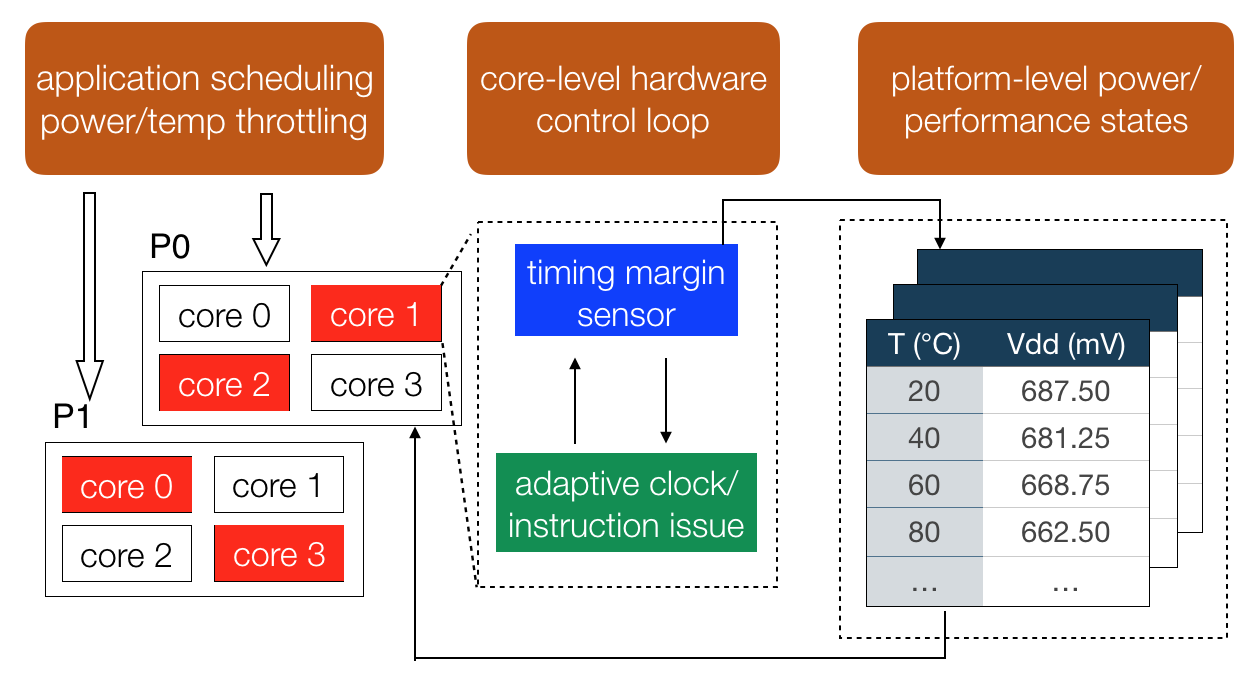
\includegraphics[trim=0 0 0 0, clip, width=\columnwidth]{graphs/intro/sys-overview.png}
  \caption{Overview of this thesis's cross-layer research on active timing margin management. We design platform-level active timing margin solution for temperature variation, characterizes state-of-the art hardware active timing margin mechanisms that deal with voltage variation, instrument core-level active timing margin fabric to expose process variation, and proposes software scheduling techniques to help these systems achieve the best power-performance gain.}
  \label{fig:framework}
\end{sidewaysfigure}

Put in the system layer context, the contribution of this thesis and the research effort I conducted to arrive at the aforementioned contributions covers circuit, architecture, and software level, illustrated by~\Fig{fig:framework}.

\textbf{At circuit and device level:} I perform hardware measurement to understand what is the granularity that timing margin sensor measures available margin, and map circuit speed/delay to temperature or voltage variation. In the \tistates proposal, the characterization of how temperature affects CMOS transistor speed, and hence available margin, is critical in building the active timing margin loop. In the voltage variation study, the dissecting of voltage noise into different components that active timing margin can, or can not deal with is built upon the understanding of how voltage affects circuit speed, using timing margin sensors.

\textbf{At architecture design level:} I propose designs that implement, or helps active timing margin perform at its best. \tistates are a set of power management states stored as tables in system firmware, which are later indexed using runtime temperature sensor readings. \tistate is essentially an evolution of classic power management states, such as P-states For voltage variation, the analysis we make points to an alternative power delivery network design which is separated into different domains, with each domain covering a few cores to minimize per-domain DC voltage drop and maximize active timing margin's voltage reduction capability.

\textbf{At system software and application level:} I propose application mapping and throttling technique on multicore systems to manage a microprocessor's DC voltage drop, with the goal of reducing total processor power or enhancing target application performance. The software solution serves as a complement to the hardware-only active timing margin mechanism and is proven by measurement to double the power reduction, or performance improvement gain.

\section{Long-term Impact}
\label{sec:intro:impact}

As Dennard scaling and Moore's law approaching their end, and general-purpose architectures becoming ripe, it is vital that the research contributed to enhancing processor power efficiency have practical long-term impact, or they perish. The long-term impact of my thesis lies in three fundamental aspects:

First, my thesis on optimizing microprocessor timing margin has wide applicability in the semiconductor industry. It is not dependent upon one processor architecture and does not affect and interfaces between hardware and software. \tistates was carried out on the GPU of an APU System-on-Chip (SoC), while the study on optimizing timing margin for voltage and process variation was conducted on a multicore platform. In principle, any processor architecture can benefit from the insights and proposals in this dissertation, including accelerators, if ultra power efficiency is desired. 

Second, the active timing margin technique has seen proven commercial success by the time this dissertation is made. When I first initiated this research topic five years ago, only a few processors are designed with active timing margin, mostly for experimenting and testing purpose~\cite{lefurgy2011active, bowman201222nm}. Today, the latest high-end chips almost all adopt this technique to squeeze out the last bit of power efficiency from silicon~\cite{tokunaga20145,grenat20145,bowman20158,webel2015robust,vezyrtzis2018droop} because of its effectiveness and convenience for implementation. In this context, our work that tries to optimize active timing margin provides a free extra mile for chip vendors to increase the efficiency gain, proving its long-term impact.

Thirdly, all results and analysis presented in this thesis are acquired from solid, real hardware measurement. Acquiring and interpreting the type of data in this thesis is very difficult, which involves a deep study of a hardware platform's internals. The measurement data not only proves the improvements and insights we made can sustain future work's tests, but also provide trustworthy, valuable guidance for other researchers who need a reference. Thus, this dissertation's impact is of high practicality.


\section{Dissertation Organization}
\label{sec:intro:outline}

The rest of my dissertation is organized as follows. 
\Sec{sec:background} introduces the basics of pipeline timing margin, prior proposals that try to optimize it, and why active timing margin is the design choice today. 
\Sec{sec:temperature}, \Sec{sec:voltage}, and \Sec{sec:process} describe the proposed active timing margin management schemes for temperature, voltage, and process variation, respectively. The work in these chapters are built upon solid characterization and analysis using hardware measurement, and the proposed work cross architecture and software design. \Sec{sec:conc} provides a retrospective and prospective view of my dissertation work. The retrospective part summarizes the principles distilled from this work on building a maximally efficient active timing margin system; the prospective part suggests next steps for generalizing our work into massive industry adoption.

\section{Previously Published Material}
\label{sec:intro:prev}

This dissertation contains materials that are previously published in peer-reviewed conferences and journals:

\textbf{\Sec{sec:background}}. The introduction on timing margin sensors, environmental sensors, and the control loop for active timing margin is a collection of the part of the materials published in the following papers: \textit{\tistates: Processor Power Management in the Temperature Inversion Region}. Yazhou Zu, Wei Huang, Indrani Paul and Vijay Janapa Reddi. In International Symposium on Microarchitecture (MICRO), 2016~\cite{zu2016tistate}; \textit{Adaptive guardband scheduling to improve system-level efficiency of the POWER7+}. Yazhou Zu, Charles R. Lefurgy, Jingwen Leng, Matthew Halpern, Michael S. Floyd and Vijay Janapa Reddi. In International Symposium on Microarchitecture (MICRO), 2015~\cite{zu2015adaptive}; \textit{Active Timing Margin Management for Maximizing Multi-Core Efficiency on an IBM POWER7+ Server}, Yazhou Zu, Daniel Richins, Charles R. Lefurgy and Vijay Janapa Reddi, submitted to International Symposium on High Performance Computer Architecture (HPCA).

\textbf{\Sec{sec:temperature}}. The design and management of active timing margin for temperature variation are based on the following paper: \textit{\tistates: Processor Power Management in the Temperature Inversion Region}. Yazhou Zu, Wei Huang, Indrani Paul and Vijay Janapa Reddi. In International Symposium on Microarchitecture (MICRO), 2016~\cite{zu2016tistate}. A modified version of this paper is also published in IEEE's annual Top Picks selection: \textit{\tistates: Power Management in Active Timing Margin Processors}. Yazhou Zu, Wei Huang, Indrani Paul and Vijay Janapa Reddi. In IEEE Micro, June 2017, 37(3):106-114~\cite{zu2017ti}.

\textbf{\Sec{sec:voltage}}. The characterization of on-chip voltage noise, as well as its active timing margin management for power saving is based on the following paper: \textit{Adaptive guardband scheduling to improve system-level efficiency of the POWER7+}. Yazhou Zu, Charles R. Lefurgy, Jingwen Leng, Matthew Halpern, Michael S. Floyd and Vijay Janapa Reddi. 

\textbf{\Sec{sec:process}}. The work on active timing margin management for multicore process variation is submitted to International Symposium on High Performance Computer Architecture (HPCA) 2019.

\textbf{Other publications}: During the length of my Ph.D., I've also worked on other related topics and made joint publications in GPU voltage analysis, Integrated Voltage Regulator analysis, etc. The co-authored papers are \textit{GPUVolt: Modeling and characterizing voltage noise in GPU architectures}. Jingwen Leng, Yazhou Zu, Minsoo Rhu, Meeta Gupta and Vijay Janapa Reddi. In International Symposium on Low Power Electronics and Design (ISLPED), 2014~\cite{leng2014gpuvolt}; \textit{GPU voltage noise: Characterization and hierarchical smoothing of spatial and temporal voltage noise interference in GPU architectures}. Jingwen Leng, Yazhou Zu and Vijay Janapa Reddi. In International Symposium on High Performance Computer Architecture (HPCA), 2015~\cite{leng2015gpu}; \textit{Ivory: Early-stage design space exploration tool for integrated voltage regulators}. An Zou, Jingwen Leng, Yazhou Zu, Tao Tong, Vijay Janapa Reddi, David Brooks, Gu-Yeon Wei and Xuan Zhang. In Design Automation Conference (DAC) 2017~\cite{zou2017ivory}; \textit{Efficient and reliable power delivery in voltage-stacked manycore system with hybrid charge-recycling regulators}. An Zou, Jingwen Leng, Xin He, Yazhou Zu, Vijay Janapa Reddi and Xuan Zhang. In Design Automation Conference (DAC) 2018~\cite{zou2018efficient}; \textit{Voltage-Stacked GPUs: A Control Theory Driven Cross-Layer Solution for Practical Voltage Stacking in GPUs}. An Zou, Jingwen Leng, Xin He, Yazhou Zu, Christopher D. Gill, Vijay Janapa Reddi and Xuan Zhang. In International Symposium on Microarchitecture (MICRO), 2018~\cite{an2018control}.
%!TEX root=../paper.tex

\chapter{Timing Margin: A Perpetual Role in Microprocessors}
\label{sec:background}

This section explains the basics of microprocessor's timing margin, and motivates why active management of timing margin is necessary to improve power efficiency. This section first goes over the necessity of timing margin in modern microprocessors. Then it enumerates the main components involved in timing margin. We end this section with a brief discussion of the working mechanism of active timing margin.

\section{The Importance of Timing Margin in Modern Microprocessors}
\label{sec:background:importance}

In the abstract form, general-purpose microprocessors are state machines that follows the von-Neumann architecture. In practice, microprocessors must be implemented in a physical form to perform the actual computation, be it add, multiply, store, or others. The physical implementation dates back to an early mechanical form as the Babbage Engine in the 1800s, and has evolved a long way to today's highly efficient electronic form as CMOS transistors. Whatever microprocessor's physical form of implementation is, they must be made and delivered with reliability guarantee, as any other human-engineered, physical instance that operate in the presence of uncertainty. Uncertainty exists because human do not have perfect control in the manufacturing and operating process. Uncertainty can be systematically biased, or purely random. Either way, it must be taken into account in a microprocessor's design, manufacturing and testing.

Modern processor's micro-architecture is pipelined for higher performance. All pipeline stages have the same time duration to complete their computing tasks, synchronized by a global clock. In each pipeline stage, circuits constructed by CMOS transistors take some time to switch and then produce a stable output electric level. In an ideal world, the circuit's switch time can be calculated using CMOS device's charge and discharge time formula given a particular supply voltage and transistor size, and pipeline cycle time should be equal to the circuit switch time, assuming all pipeline stage have the same switch time. However, in the real world, circuit switch time can have lots of uncertainty caused by, for instance, imperfect transistor size during manufacturing, transistor performance variation due to heating, or imperfection in supply voltage, etc. The uncertainty could make circuits complete their jobs faster, or slower than the time duration calculated by theoretical formulas. To assure all circuits have plenty of time to get their jobs completed, pipeline cycle time is always longer than the theoretical circuity switch time, the added time duration in clock cycle is called \textit{timing margin}, as illustrated in~\Fig{fig:timing-margin}.

A good analogy of microprocessor pipeline's timing margin in everyday life is the relationship between cars and lanes. In an ideal world, a lane would have the same width as a car because car would strictly obey the orbits of the lane. Yet, in the real world, lanes are always (much) wider than cars because cars often deviate from lane orbits by some error, or uncertainty. The deviation uncertainty may be caused by human driver's improvisation, or the inherent control error of the vehicle (e.g., a mismatch between the left and right tires). The extra space between a lane and a car allows the car to correct itself and stay on track. The extra room between lane width and car width works just like how pipeline timing margin protects against circuit's timing uncertainty.

\begin{figure*}[t]
\centering
\subfloat[Static timing margin.] {
  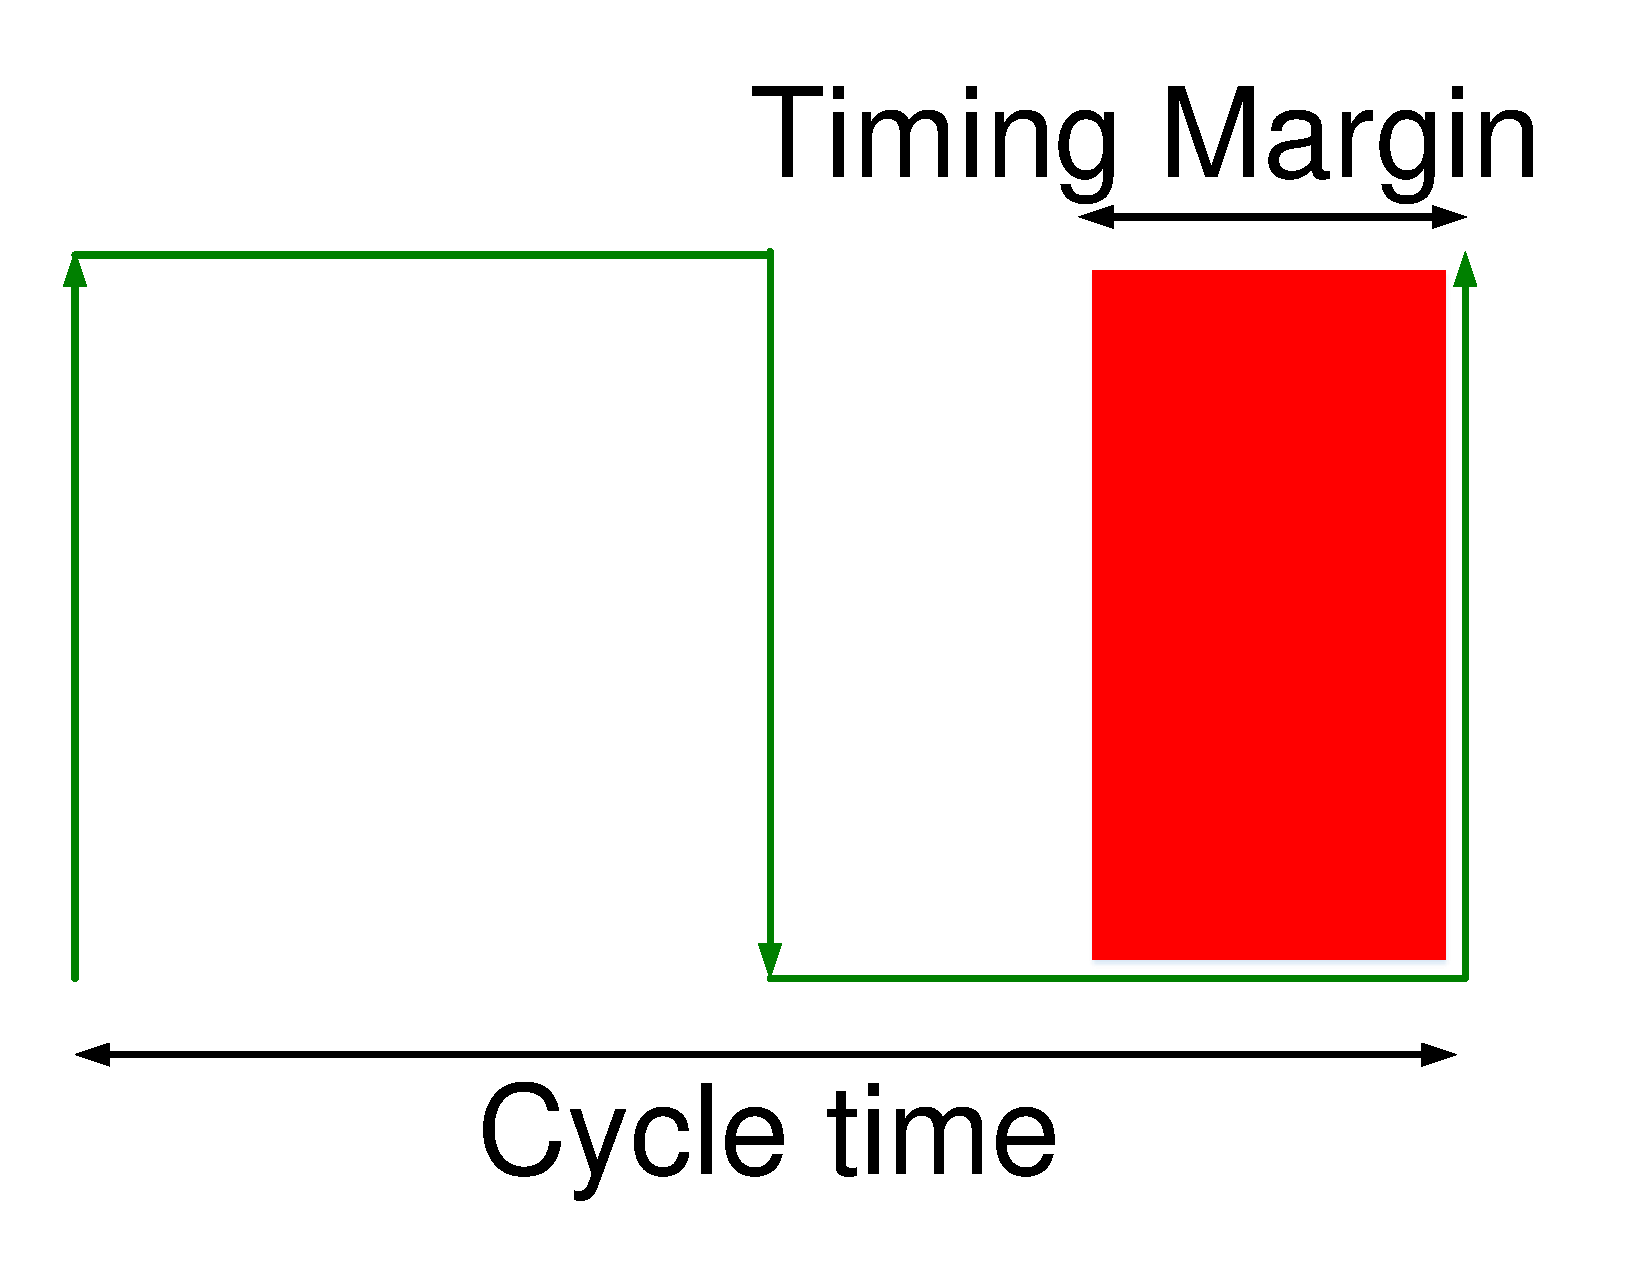
\includegraphics[trim=0 0 0 0,clip,width=.25\linewidth]{graphs/background/timing-margin.pdf}
  \label{fig:timing-margin} 
}
\hfill
\subfloat[Voltage guardband.] {
  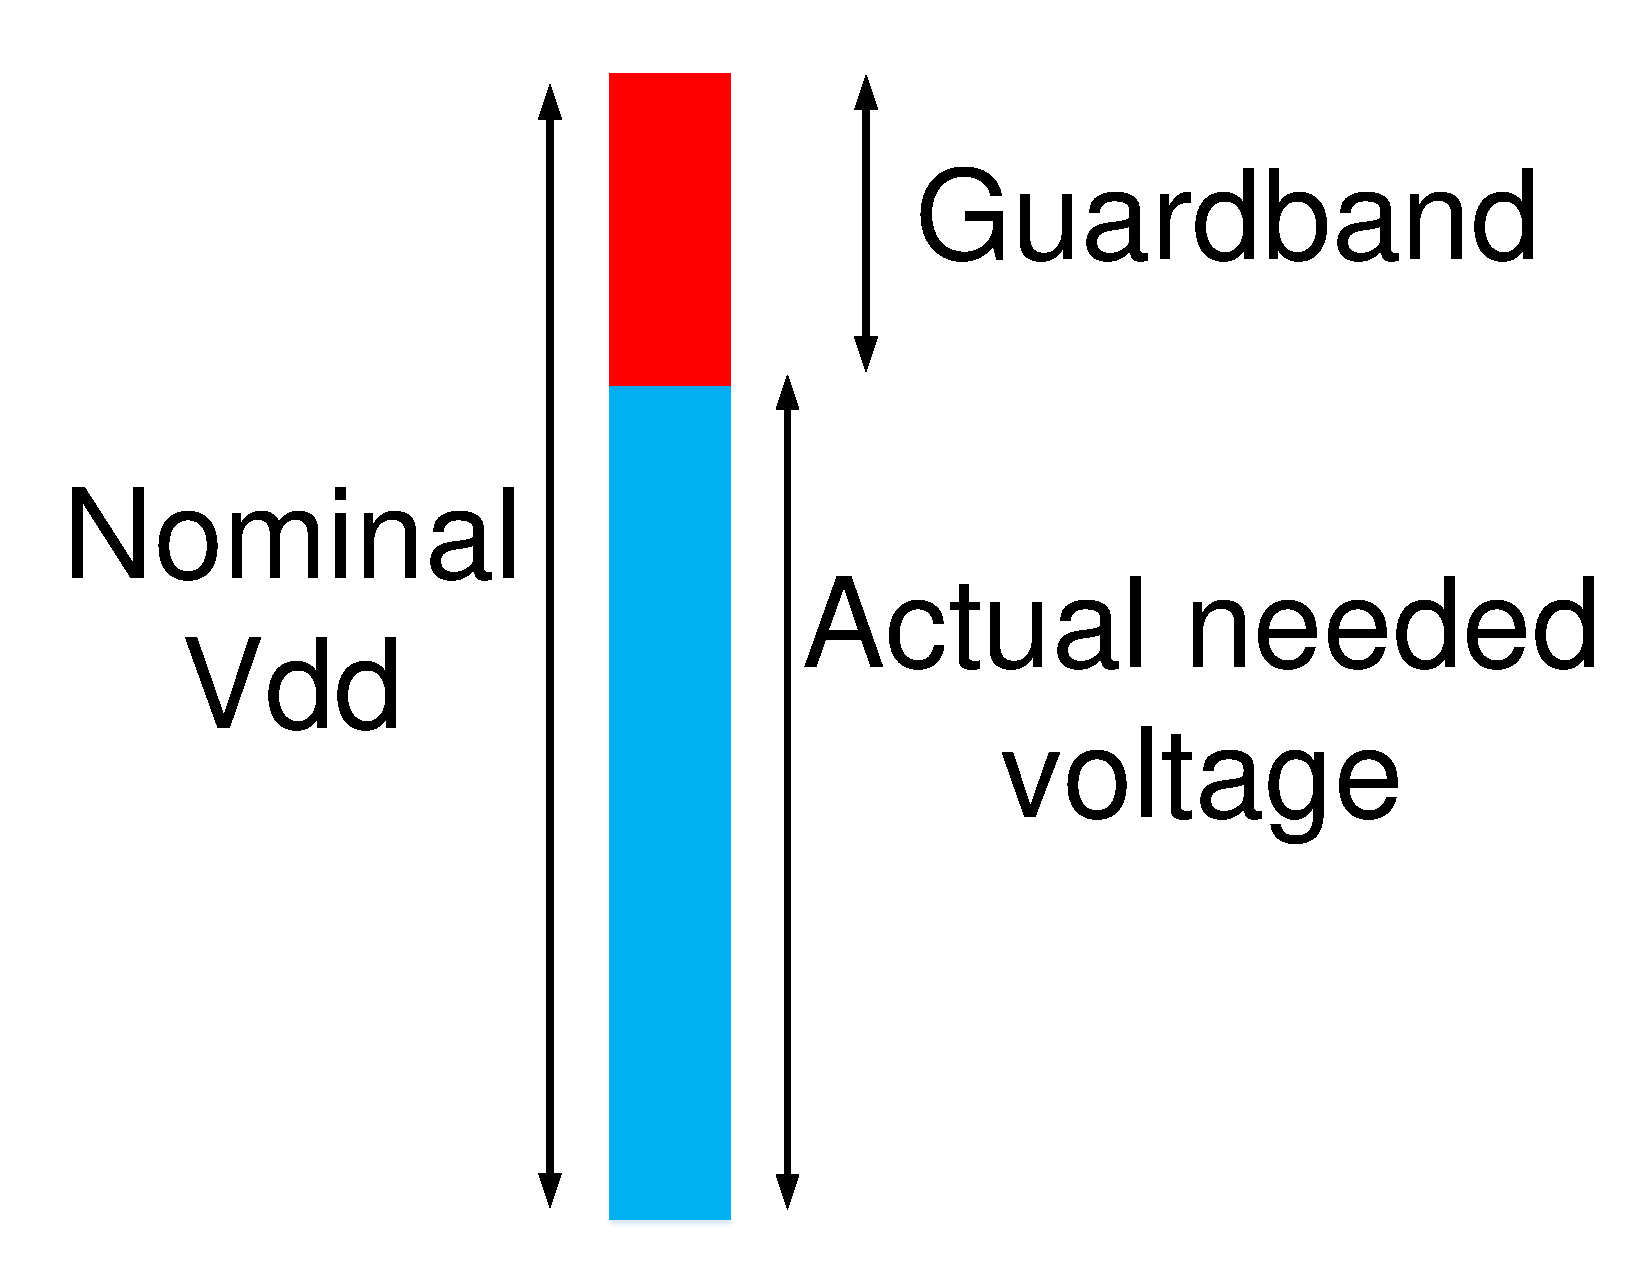
\includegraphics[trim=0 0 30 0,clip,width=.25\linewidth]{graphs/background/voltage-guardband.pdf}
  \label{fig:voltage-guardband} 
}
\hfill
\subfloat[Active timing margin.] {
  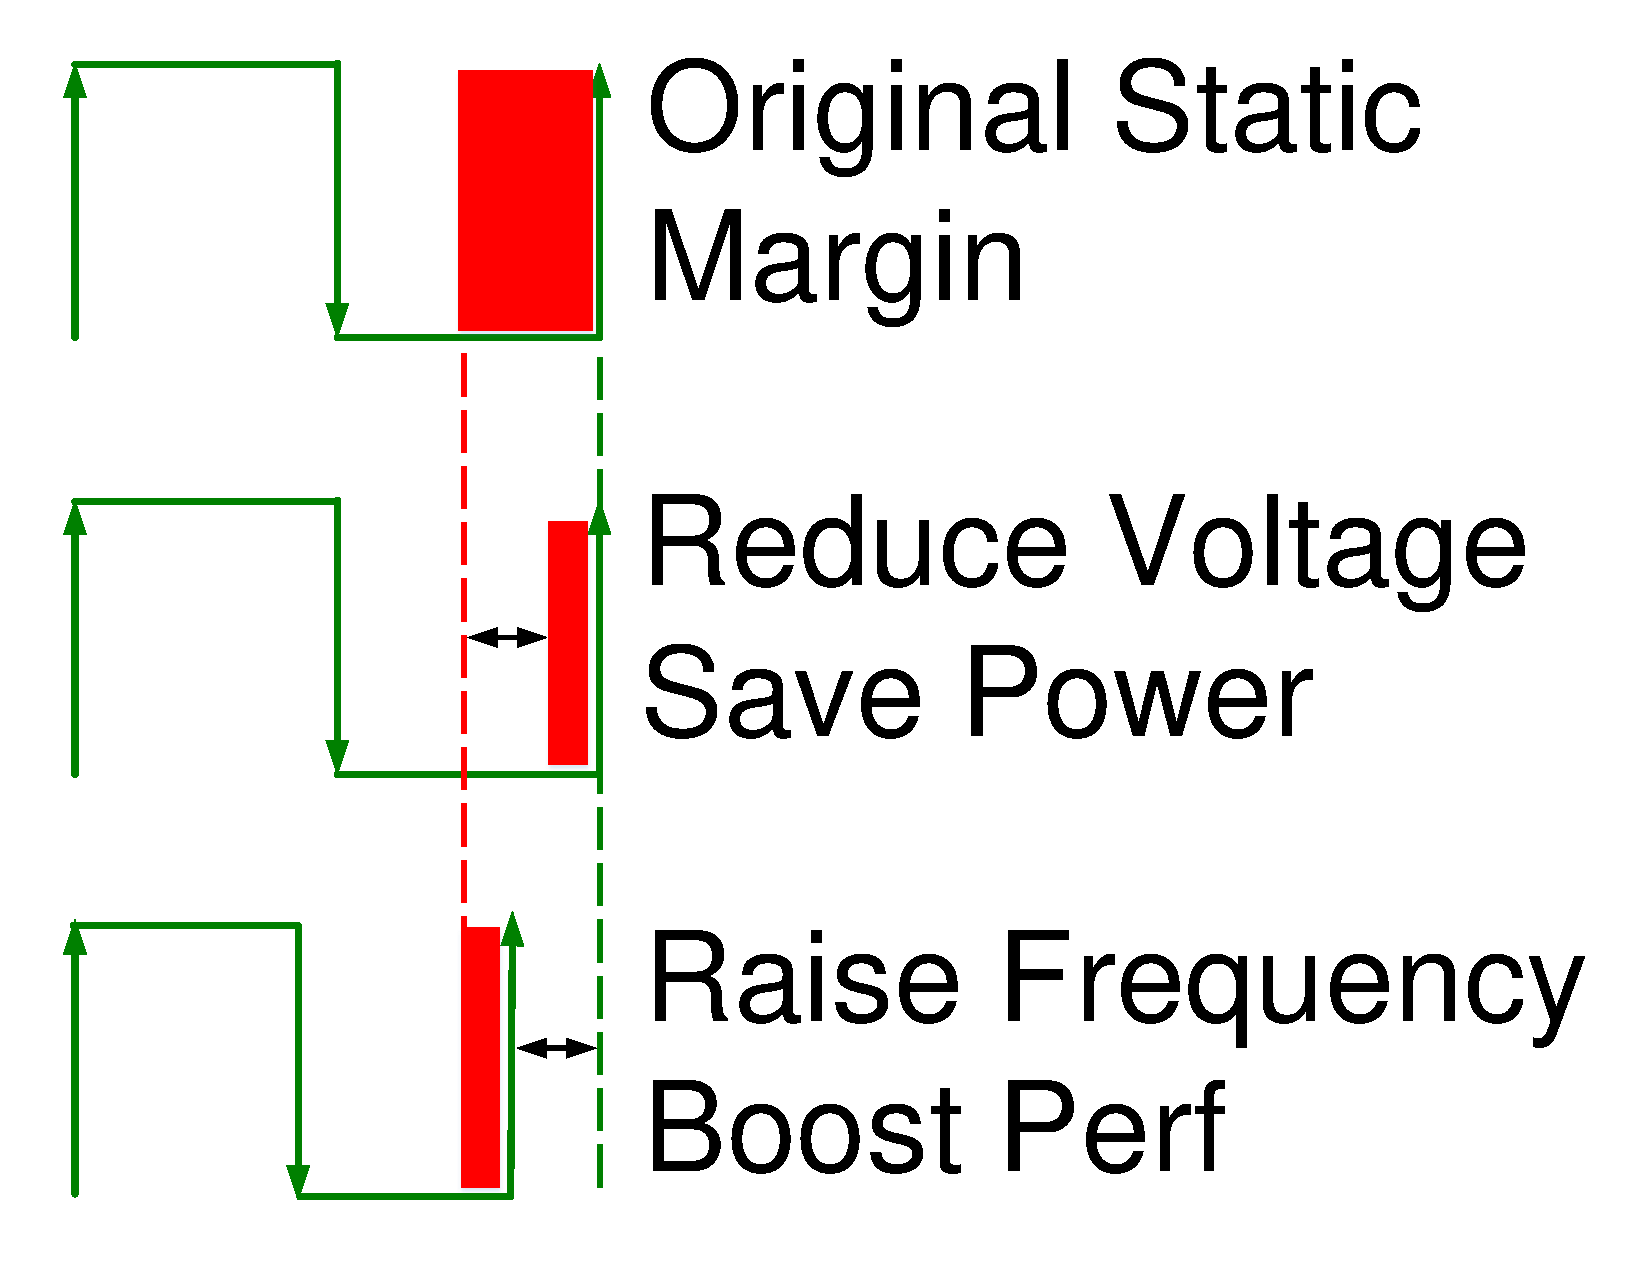
\includegraphics[trim=0 0 0 0,clip,width=.25\linewidth]{graphs/background/adaptive-margin.pdf}
  \label{fig:adaptive-margin} 
}
\caption{Timing margin ensures reliability by creating extra room in pipeline's clock cycle time. It can be delivered by providing extra voltage, known as the voltage guardband. Active timing margin improves from conventional static margin with tighter clock cycle by overclocking or undervolting.}
\end{figure*}

Failing to take circuity's performance uncertainty into account can lead to the microprocessor malfunction. One good example is the rowhammer problem discovered in DRAM chips recently~\cite{kim2014flipping}. In DRAM chips, stressing one row can cause the row's adjacent cells to leak charge quicker than usual, and eventually causes a bit flip which may have serious repercussions. To protect against this situation, DRAMs need to provide ample headroom to tolerate the uncertainty in a cell's charge leakage time, such as by refreshing cells quicker which is a form of timing margin. Though DRAM is not exactly the same as a microprocessor, this case illustrates the importance of timing margin in CMOS chips.

\section{Major Consumers of Microprocessor's Pipeline Timing Margin}
\label{sec:background:components}

Timing margin can be implemented as tuning supply voltage slightly higher, which makes circuits operator faster and thus leaving some timing slack, or tuning the frequency slightly slower, which makes cycle time longer. These two methods are equivalent to each other. The former approach is widely known as \textit{voltage guardband} as described in \Fig{fig:voltage-guardband}. We explore both methods in this thesis.

In today's CMOS chips, the amount of timing margin needed to ensure microprocessor reliability is often excessively high because of the various sources of timing uncertainty. Prior art has tried to quantify the magnitude voltage guardband on GPUs. In~\cite{leng2015safe} researchers report around 20\% voltage guardband from commercial products, which can amount to more than 25\% power and energy wastage. The wastage is significant not only because of the power and energy it consumes, but also because today's microprocessors are inherently power limited, and wasting power means limiting processor performance. Therefore it is imperative that we investigate what leads to timing uncertainty and consumes timing margin. 

\paragraph{Temperature variation} is one important source of timing uncertainty. When temperature changes, transistor performance varies because temperature variation alters the activity level of the particles in the semiconductor material, which changes transistor switch speed and circuit completion time.In practice, processor temperature variation is unavoidable because during workload run the charge and discharge of semiconductor transistors inevitably raises temperature. Depending on workload intensity, the temperature profile of the chip varies temporarily and spatially, affecting circuit timing. To tolerate timing uncertainty caused by temperature variation, margin must be added in the cycle time. In \label{sec:tistate} we perform an in-depth study on how temperature affects timing uncertainty and device architecture and system level mechanisms to combat against it.

\paragraph{Voltage variation} is a complex source of timing uncertainty. It is caused by the interaction between the parasitics of the power delivery subsystem of a microprocessor and the varying power draw under workload stress. \Fig{fig:pdn-model} gives an overview of the physical mechanism of voltage variation.

\begin{figure*}[t!]
  \centering
  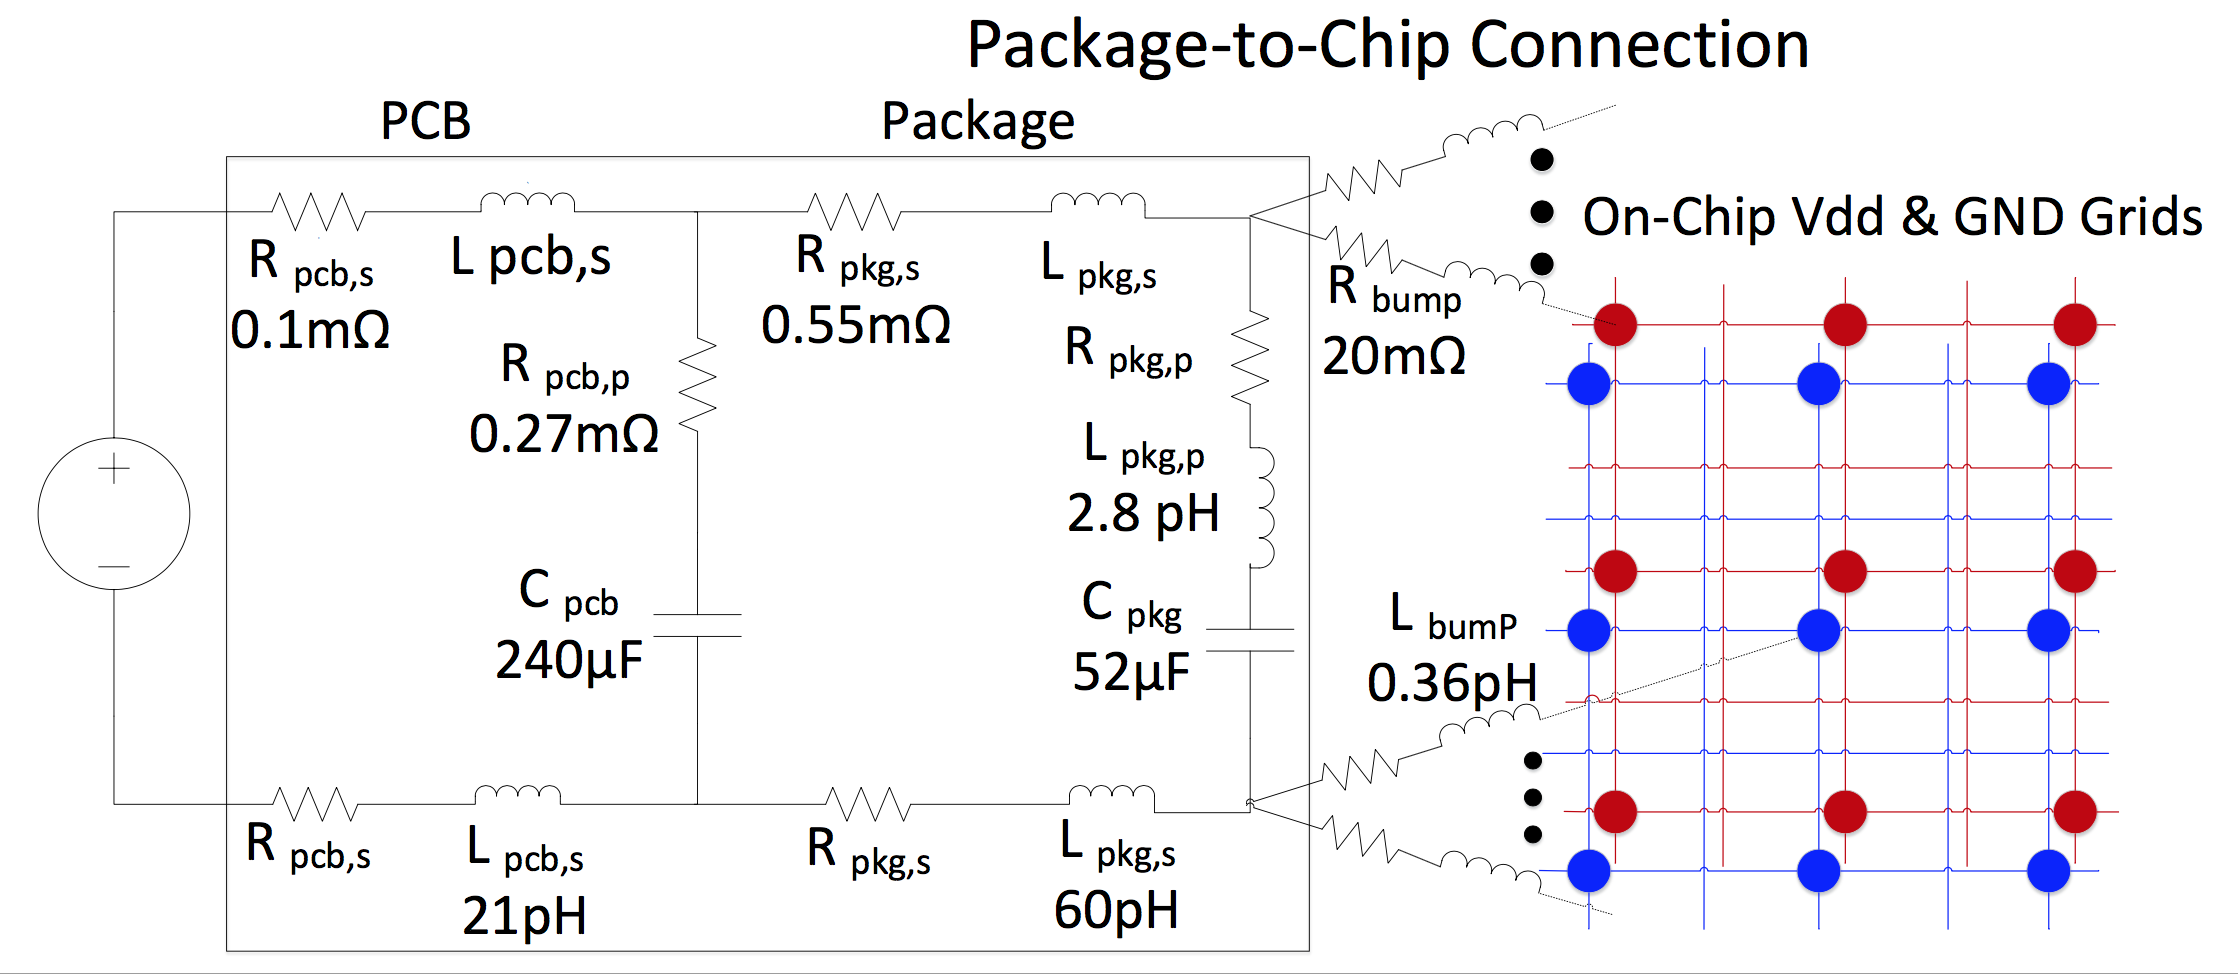
\includegraphics[trim=0 0 0 0,clip,width=0.8\linewidth]{graphs/background/pdn-model.png}
  \caption{An electrical model of the power delivery path from the voltage regulator module (VRM) to on-chip transistors. Impedance of different types exist on this path because of the electrical parasitics on the motherboard as well as inside the package. IR drop and the L$di/dt$ effect are caused by these parasitics.}
  \label{fig:pdn-model}
\end{figure*}

The supply voltage delivered to the CMOS transistors has lots of noise because the path from the source of voltage supply to the end transistors has lots of parasitics. Typically, the power supply subsystem can be modeled as four parts: the voltage regulator module, electrical parasitics on the printed circuit board, electrical parasitics at the package contact points, and on-die power delivery network. Each part has its own resistive, capacitive, and inductive parasitics that impede the transmission of voltage. These parasitics exist because the power delivery subsystem is made of real, physical materials - on-chip and off-chip wires have resistance even the magnitude can be small, wires can form loops by chance and create inductive impedance, the alignment between wires and the added decoupling capacitors create capacitance, etc.

Resistive parasitics cause supply voltage's IR drop following Ohm's law. Higher power causes higher IR drop. Inductive and capacitive parasitics further worsen supply voltage with the $di/dt$ effects. $di/dt$ effect happens when there is rapid change in the current draw, or power consumption of the transistors. $di/dt$ effect is happens rapidly, typically over tens of cycles, yet very rarely, making it hard to tract and especially dangerous. The combined IR drop and $di/dt$ effects make the supply voltage experienced by transistors very noisy. This adds uncertainty to the speed of microprocessor pipeline circuit. Therefore, timing margin, must be added to tolerate various voltage variation effects.

\paragraph{Process variation} is another source of uncertainty in circuit performance. Unlike temperature and voltage variation which change dynamically during runtime, process variation is a static effect that is formed during chip's manufacturing process, i.e., lithography. During lithography, noise can occur because the lithography instruments cannot perfectly control the various lithography steps, such as etching and doping. Wire width, transistor gate width and length can be etched with noise. Dopant density can deviate from the ideal density level. All these effects make transistor and wire's performance deviate from the ideal case, and make the speed of different transistors and wires differ. A microprocessor's performance is determined by the slowest part of the chip. The result is that faster circuits are forced to have some amount of timing margin because it is synchronized using the same clock as the slow circuits. We leave the study of timing margin caused by process variation to future work.

\paragraph{Other noisy effects} such as transistor aging, processor testing inaccuracy also contribute to pipeline circuit timing uncertainty. However, these effects' intensity is not as strong as temperature, voltage, and process variation aforementioned, and the condition for it to occur is too extreme. For this reason, we leave out these effects in this proposal and focus on voltage, temperature and process variation.

\section{The Need for Active Timing Margin and Its Management}
\label{sec:background:motivation}

Traditionally, timing margin is fixed during chip design stage, the process of which follows a \textit{worst-case} design approach. In other words, the amount of timing margin must be able to tolerate the most extreme conditions that slow down microprocessor circuits, such as very heavy $di/dt$ voltage droops, very large IR drop caused by high power workloads, and unusual operating temperature that degrade transistor performance. The aggregate corner case of all effects determine how much timing margin is added to the chip.

The worst-case design approach described above is straightforward and easy to implement. Its design complexity is very low - simply raising voltage by some guardband value. It is also very robust in that all the worst-case conditions are tested and protected, so any timing uncertainty caused by any workload load condition should be tolerated because workload-induced uncertainty can be no worse than the hand-tuned worst-case condition. For years the worst-case timing margin approach has been the adopted and the down side of it has not drawn too much attention in microprocessor design and management because its voltage overhead is not as significant as other architecture performance or power issues. Yet, as various microarchitecture approach develops towards maturity and semiconductor technology scales to its limit, the research community is realizing that this static timing margin has become one of the golden opportunities that can be leveraged to squeeze power efficiency out of the underlying chip.

The main problem of the worst-case timing margin approach is that it is a static mechanism and overprovisions timing margin/voltage guardband resource most of the time. As an example, measurement on GPUs shows that most real-world programs do not need the full amount of voltage guardband. The reason is that the timing margin decided based on worst-case conditions are far different from the typical operating environments - workloads do not create extremely high or low temperature most of the time, nor do they invoke rapidly changing power variations often. These extreme conditions can only be met by specially built stress workloads like power and voltage virus programs, which involves non-trivial systematic design effort~\cite{kim2012audit,bertran2014voltage,bertran2012systematic}.

Real-world workloads often switch between different phases, and different phases may utilize the timing margin in very different manners. A program may enter a power hungry phase for a while, which induces heavy IR drop and raises chip temperature, and ultimately slows down transistors and consumes the timing margin heavily. After the computing in this phase is finished, the same program may enter a low power IO phase where circuit timing delay is small because of the low power, low IR drop, and mediate temperature levels. In this phase, timing margin is mostly wasted. The static, worst-case timing margin approach ignores workload dynamism and only targets the extreme situations, leaving timing margin unused and wasted most of the time. 

To work around the inefficiency of the worst-case static margin approach, timing margin must dynamically track workload behavior, check when workloads need timing margin, and provision it just-in-time. When workloads do not need high timing margin, voltage can be tuned down or frequency can be tuned up to save power or boost performance as illustrated in \Fig{fig:adaptive-margin}. This is the principle of \textit{active timing margin}. Figure xyz illustrates this idea with an $di/dt$ effect.

\begin{figure}[t!]
\captionsetup[subfloat]{width=0.4\textwidth}
\centering 
\subfloat[Static timing margin tolerates worst-case $di/dt$ effect with fixed low frequency.]
{
  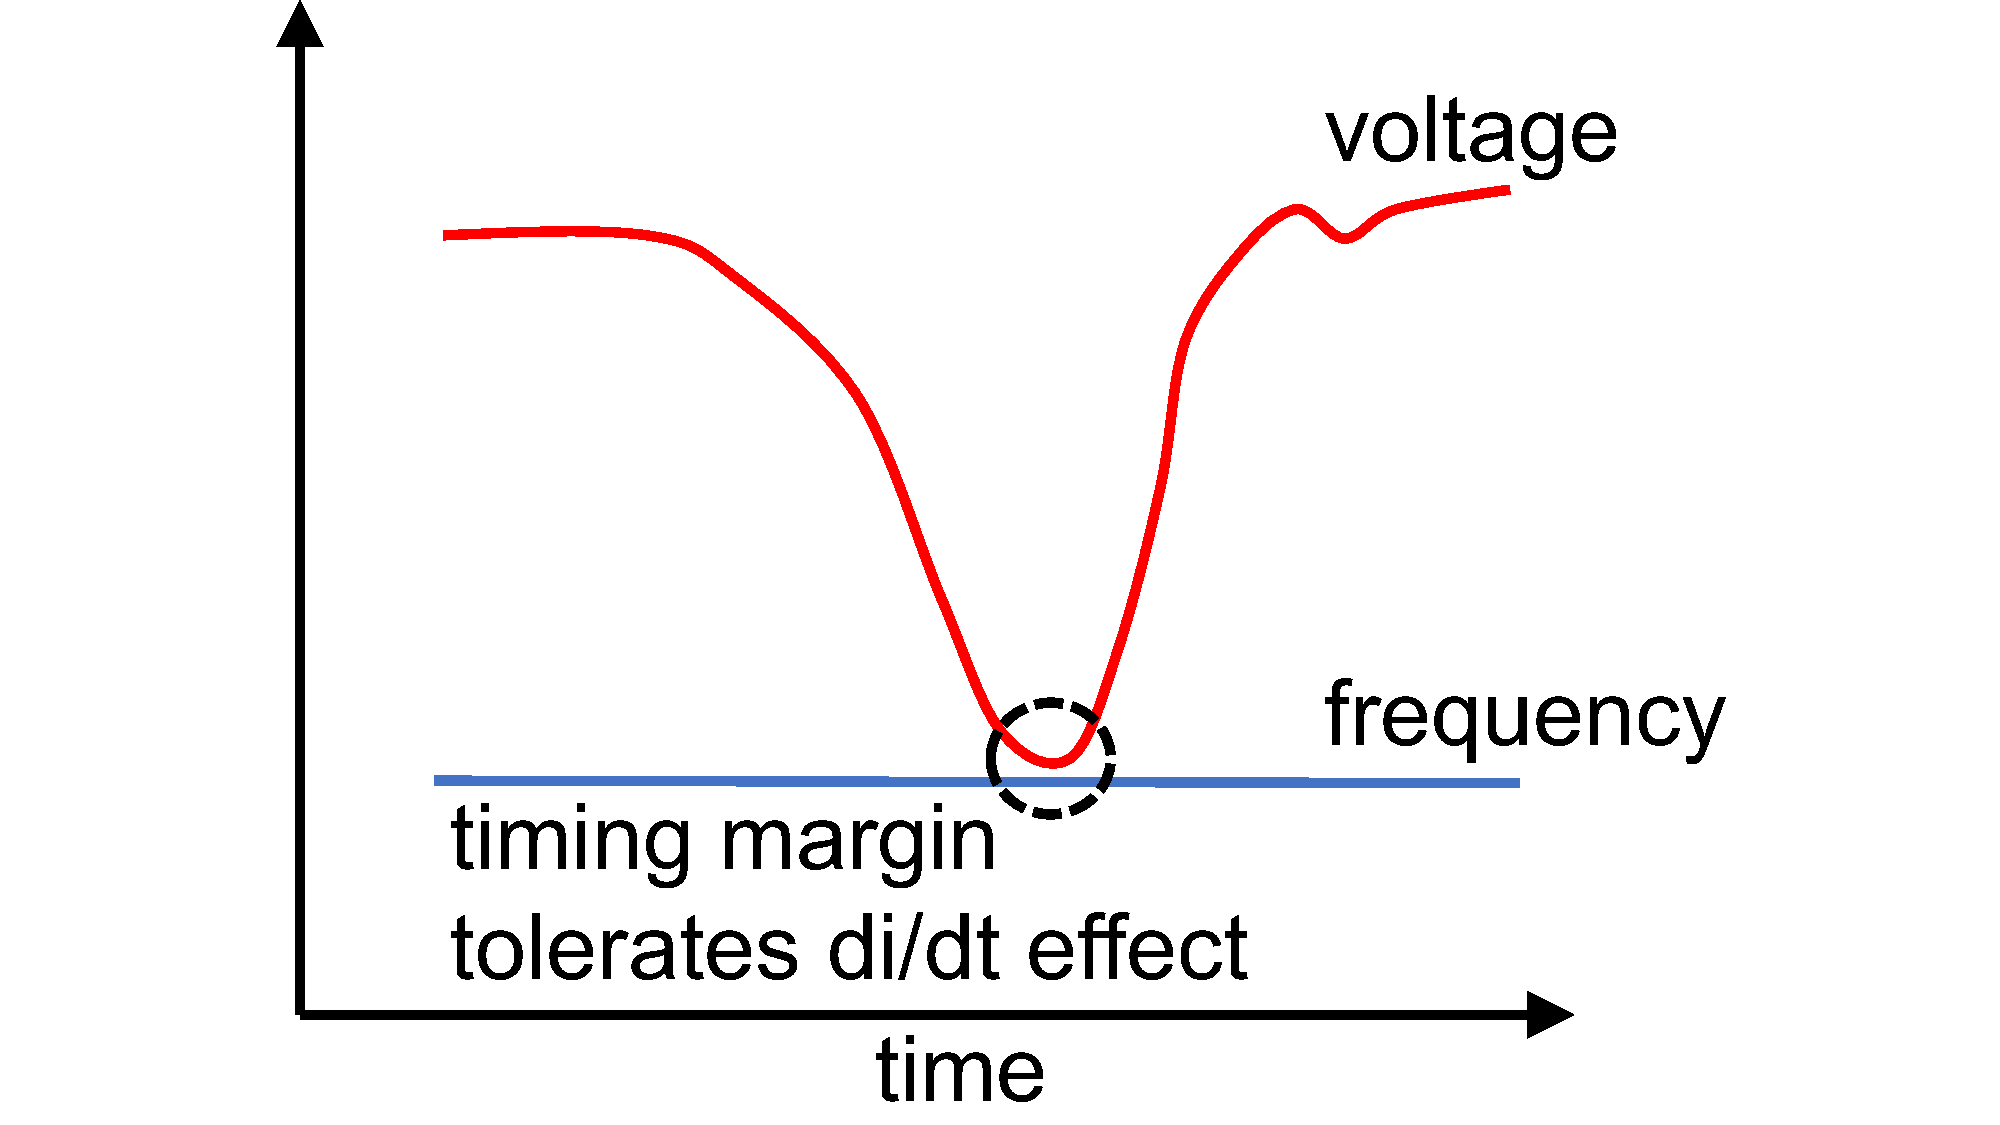
\includegraphics[trim=0 0 0 0,clip,width=0.47\linewidth]{graphs/background/didt-diagram1.pdf}
  \label{fig:didt-diagram1}
}
\subfloat[Active timing margin tolerates $di/dt$ effect by making frequency track voltage variation.] 
{
  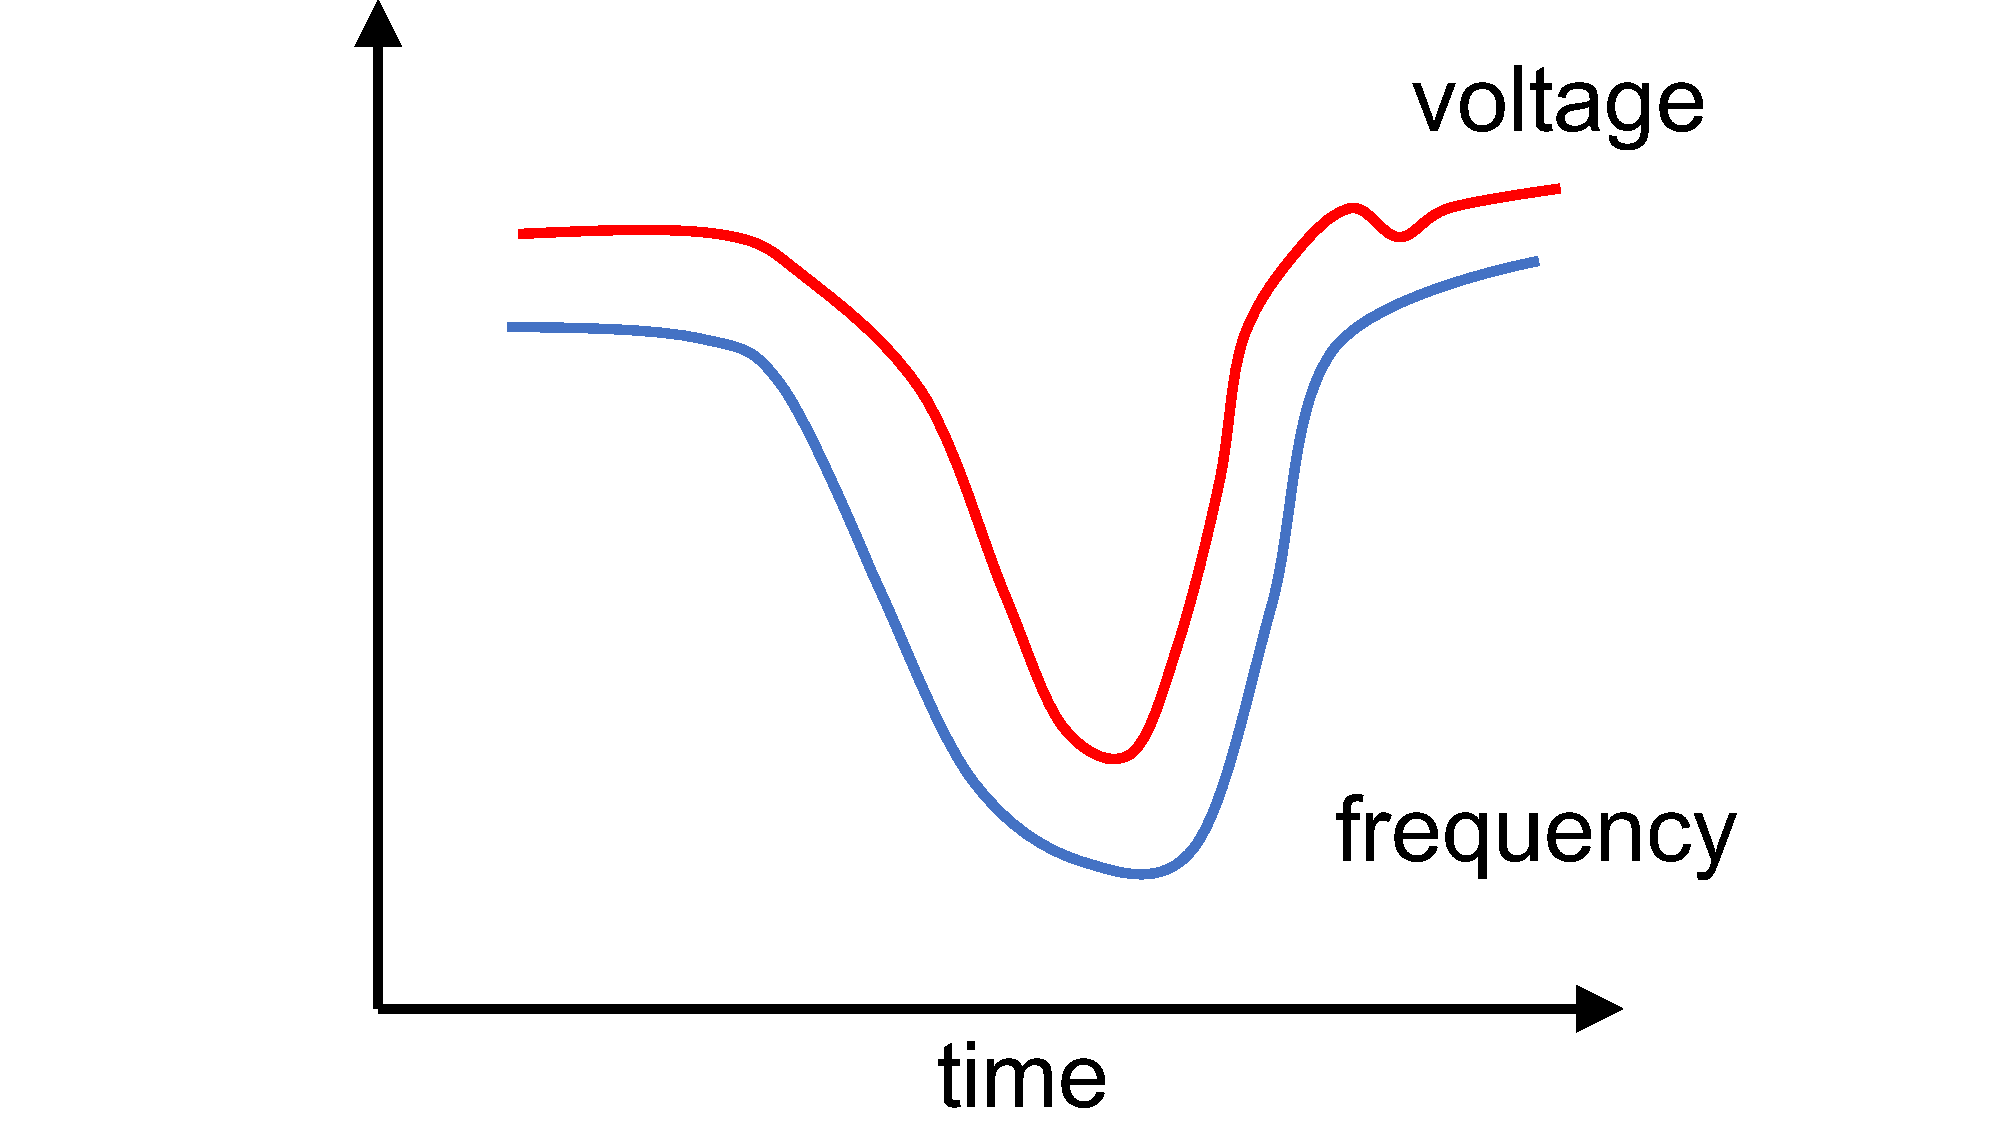
\includegraphics[trim=0 0 0 0,clip,width=0.47\linewidth]{graphs/background/didt-diagram2.pdf}
  \label{fig:didt-diagram2}
}
\caption{Active timing margin protects $di/dt$ effect by making frequency/clock cycle track supply voltage, which improves performance and reduces timing margin wastage.}
\vspace{-0.2in}
\end{figure}

In Figure \Fig{fig:didt-diagram1}, a heavy voltage droop caused by strong $di/dt$ effect slows down circuits, and necessitates some amount of timing margin to protect against it. The static margin does tolerate the $di/dt$ effect with a fixed, low frequency. However, only small voltage ripple occurs on the power delivery network when heavy $di/dt$ effect is not in place. During these periods, large timing margin is not needed, yet the static approach still provisions the timing margin set by the worst case, wasting a lot of performance under the same voltage. 

In \Fig{fig:didt-diagram2}, active timing margin dynamically adjust clock frequency to match the magnitude of voltage variation. When the $di/dt$ effect occurs, clock frequency ramps down quickly to provide the need timing margin. When there's no $di/dt$ effect, clock frequency stays at a higher level to reclaims the unused timing margin. Overall, the system enjoys higher performance.

Active timing margin bases itself on sensory detection of how emergent, or how much timing margin is used, and dynamically adjusts the amount of timing margin to match workload's need. When timing margin is used heavy, such as the case of strong IR drop, strong $di/dt$ effect, or on a core made of slow transistors, timing margin is added to provide extra space for safety. When timing margin is not used much, such as a light load workload phase, timing margin is shrunk to enhance efficiency. 

Along this line, we device active timing margin mechanism if solution corresponding to a particular effect does not exist yet, and explore active timing margin's implications for architecture design and system operation. We inspect possible ways to assist active timing margin to maximize its potential power efficiency benefits, and show that architecture and software cooperations are as important as implementing active timing margin itself to unlock the full opportunity hidden in timing margin.
%!TEX root=../paper.tex

\chapter{Ti-states: Active Timing Margin Management in the Temperature Inversion Region}
\label{sec:temperature}

Temperature has an intuitive impact on circuit speed, timing, and pipeline timing margin because CMOS transistor performance varies under different chip temperature levels. Conventionally, chip designer's view is that transistor slows down a lot under a higher temperature, so timing margin is set against the worst-case high temperature. However, we find this view no longer holds in today's CMOS technologies owing to an effect called \textit{temperature inversion}. In today's state-of-the-art technology nodes, the temperature inversion effect is the \textit{major temperature-related effect} that changes circuit performance and hence affect pipeline timing margin, and this phenomenon induces high speed variation. Therefore, we devise an active timing margin solution for temperature variation, with a focus on the temperature inversion effect, and explore system-level management scheme to achieve the highest power saving.

Formally, temperature inversion refers to the phenomenon that in certain voltage regions transistors speed up and operate faster at a higher temperature. \Fig{fig:motivation1} illustrates the temperature inversion effect we measured on an AMD\textsuperscript{\textregistered} A10-8700P processor~\cite{munger2016carrizo}. It shows the normalized circuit performance under different temperature with respect to a 0\C baseline. At 1.1 V, as temperature increases, circuit performance becomes \textit{slightly} slower at 80\C, as expected from conventional wisdom. However, at 0.7~V circuit becomes much faster as temperature increases to 80\C owning to the temperature inversion phenomenon. Between 1.1 V and 0.7 V there exists a special {\it inflection voltage} level at 0.9~V where circuit speed remains almost constant at all product specified temperatures. 

\begin{figure}[t!]
\captionsetup[subfloat]{width=0.4\textwidth}
\centering 
\subfloat[Under low voltage, temperature inversion increases circuit performance.]
{
  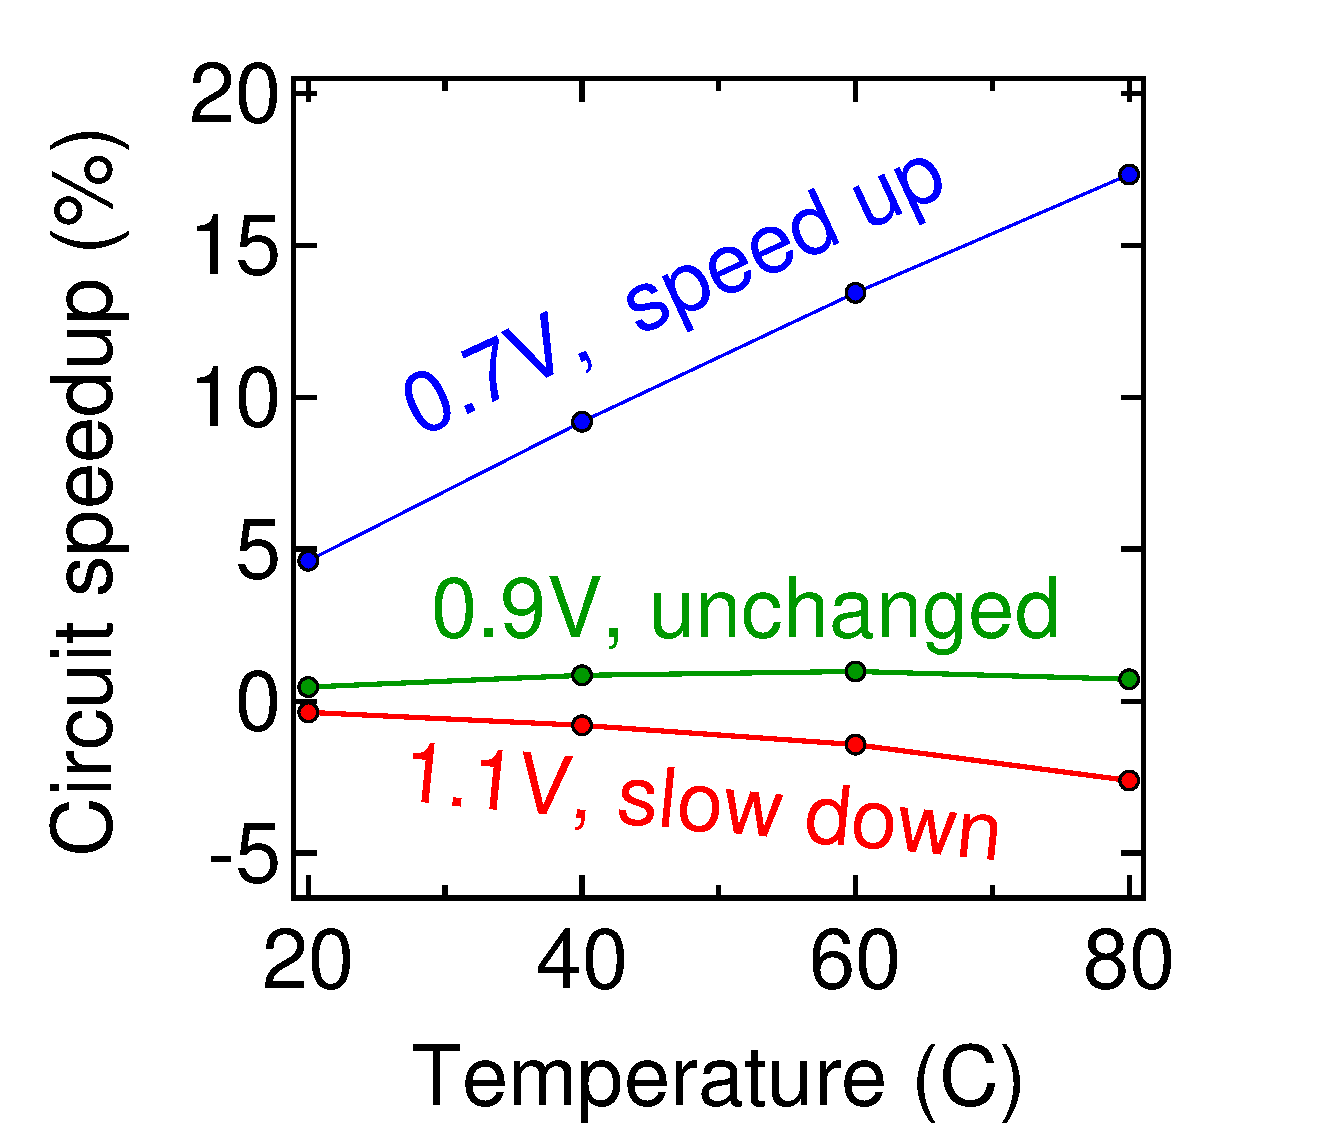
\includegraphics[trim=20 0 0 20,clip,width=0.35\linewidth]{graphs/temperature/motivation1.pdf}
  \label{fig:motivation1}
}
\hspace{0.4in}
\subfloat[Temperature inversion's inflection voltage approaches nominal supply.] 
{
  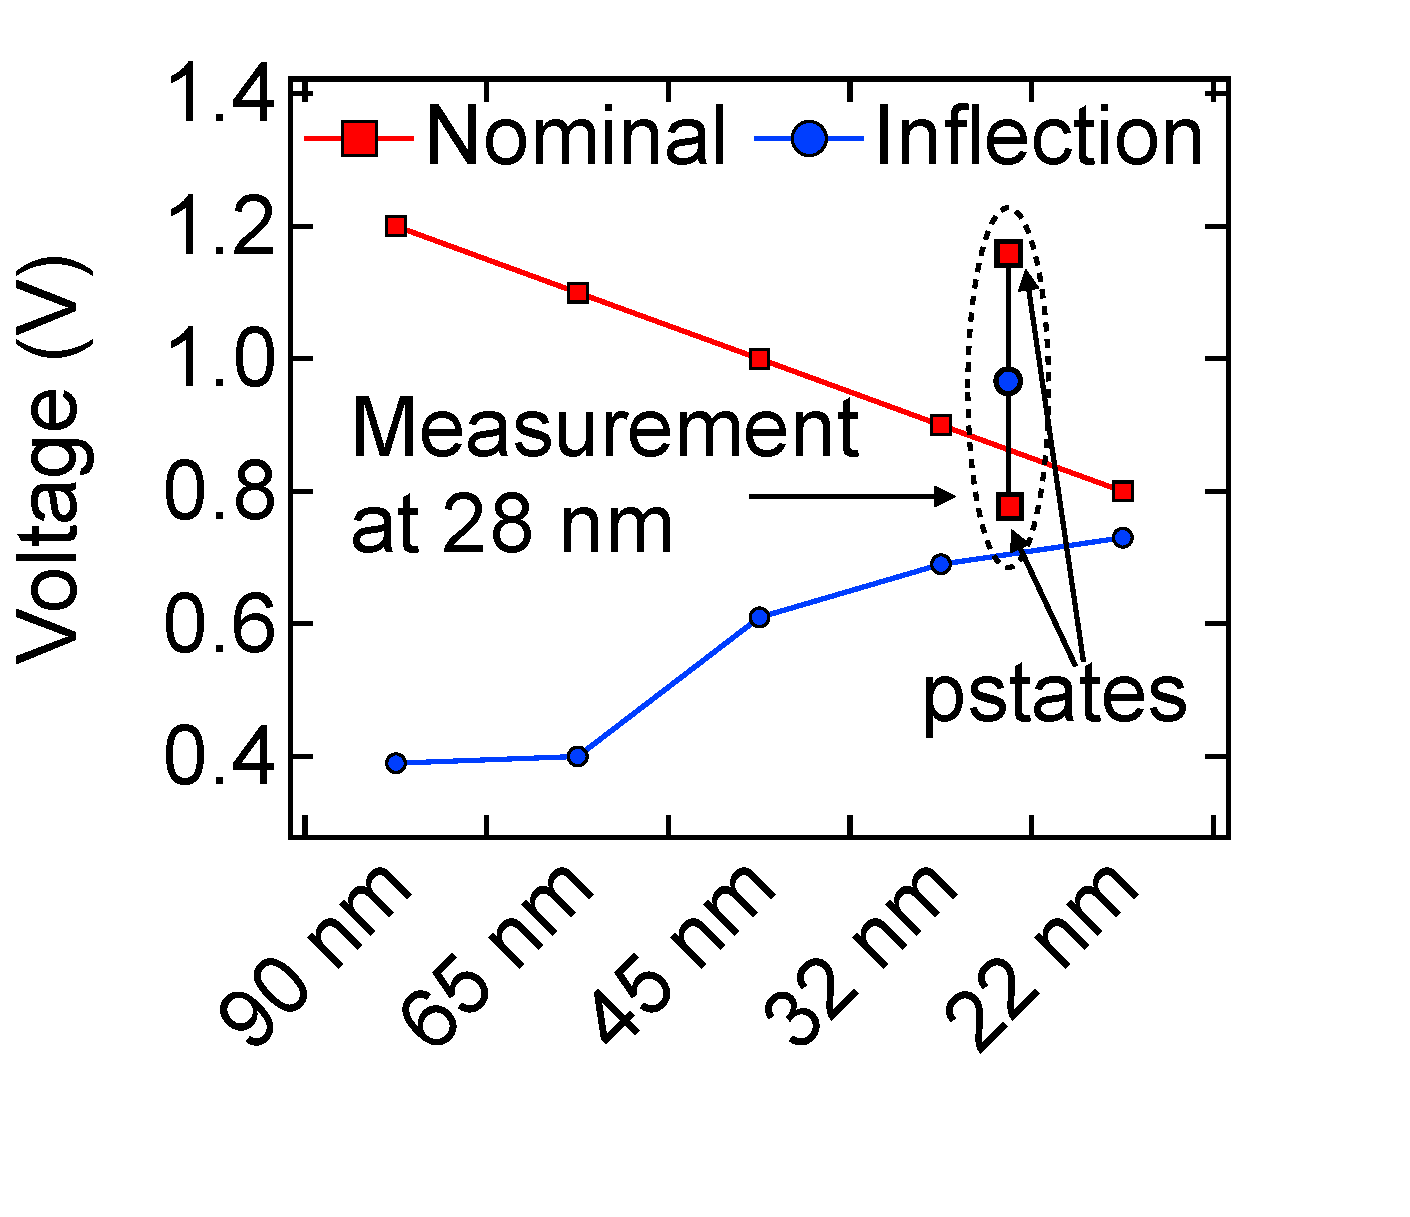
\includegraphics[trim=10 40 40 20,clip,width=0.35\linewidth]{graphs/temperature/motivation2.pdf}
  \label{fig:motivation2}
}
\caption{Temperature inversion is having more impact on processor performance as technology scales.}
\label{fig:motivation-plots}
\vspace{-0.2in}
\end{figure}

At a high level, the reason why temperature inversion occurs is a resulting of two fundamentally conflicting effects - when the temperature increases both carrier mobility and threshold voltage decrease. Carrier mobility decrease causes devices to slow down while threshold voltage reduction causes the devices to speed up. Temperature inversion happens in the region where the supply voltage is low enough to make the second factor (i.e., threshold voltage reduction) dominate, which is 0.7 V in~\Fig{fig:motivation1}. Otherwise, the devices slow down at the higher temperature, degrading performance as in the case of 1.1 V. 

In the past, temperature inversion has been safely discounted by processor designers because the nominal supply voltage at which this effect starts to occur is too low in prior technologies. At 250~nm, when temperature inversion was first discovered, the inflection voltage was more than 1.5~V lower than the nominal supply voltage~\cite{park1995reversal,bellaouar1998supply,dasdan2006handling}. With such a wide margin of separation, temperature inversion does not interfere with the processor's normal operating voltage region.

However, with technology scaling, today's processors are operating close to the temperature inversion's voltage region. Thus, the impact of this effect can no longer be safely discounted. \Fig{fig:motivation2} shows a detailed device analysis based on predictive technology models~\cite{wolpert2012temperature,zhao2006new}. As technology scales down from 90~nm to 22~nm, the inflection voltage increases with smaller feature sizes. At the 32~nm node, the inflection voltage is predicted to closer to the nominal supply voltage. Scaling into future FinFET and FD-SOI devices with smaller feature sizes, it is likely that temperature inversion will occur for all of a processor's operating voltage range~\cite{lee2014dynamic,cai2015tei}.

Silicon measurements performed on the AMD\textsuperscript{\textregistered} A10-8700P processor confirm this behavior in practice. At the 28~nm node, the inflection voltage in~\Fig{fig:motivation2} falls within the range of the processor's different P-states. The integrated GPU's highest P-state is only slightly above the inflection point. 

The fact that temperature inversion is the major temperature-related effect that varies circuit speed and timing margin today, and the fact that it has been neglected by the architecture community in the past make it imperative to thoroughly investigate the potential implications temperature inversion imposes on timing margin and architecture design. For this reason, we focus on exploiting temperature inversion for actively provisioning timing margin depending on runtime temperature level and transistor temperature inversion intensity. The rest of this section is organized as follows: \Sec{sec:temperature:setup} explains our experimental setup, \Sec{sec:temperature:characterize} systematically characterize how temperature affects circuit speed in contemporary microprocessors, \Sec{sec:temperature:tistate} proposes our \tistate solution for active timing margin, \Sec{sec:temperature:manage} discusses how to manage systems equipped with \tistates, and \Sec{sec:temperature:related} addresses related work.

\section{Experimental Setup}
\label{sec:temperature:setup}

In this subsection, we provide an overview of the experimental platform to study temperature inversion, including the chip under study and our temperature control mechanism. In particular, we explain the timing margin sensor we use, which serves as \textit{power supply monitor} in this chip. Timing margin sensor is the key element of our work.

\begin{figure}[t!]
  \centering
  \begin{minipage}{0.45\linewidth}
    \centering
                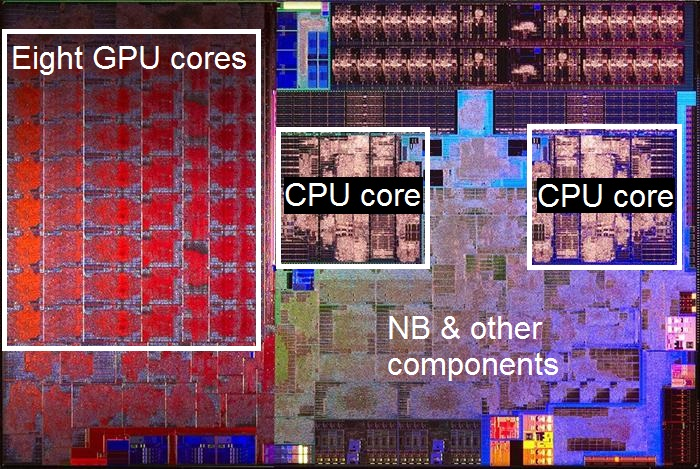
\includegraphics[trim=0 0 0 0,clip,height=1.5in]{graphs/temperature/carrizo-die.jpg}
                \caption{Die photo of the A10-8700P SoC.}
                \label{fig:die-shot}
  \end{minipage}
\hfill
  \begin{minipage}{0.45\linewidth}
    \centering
                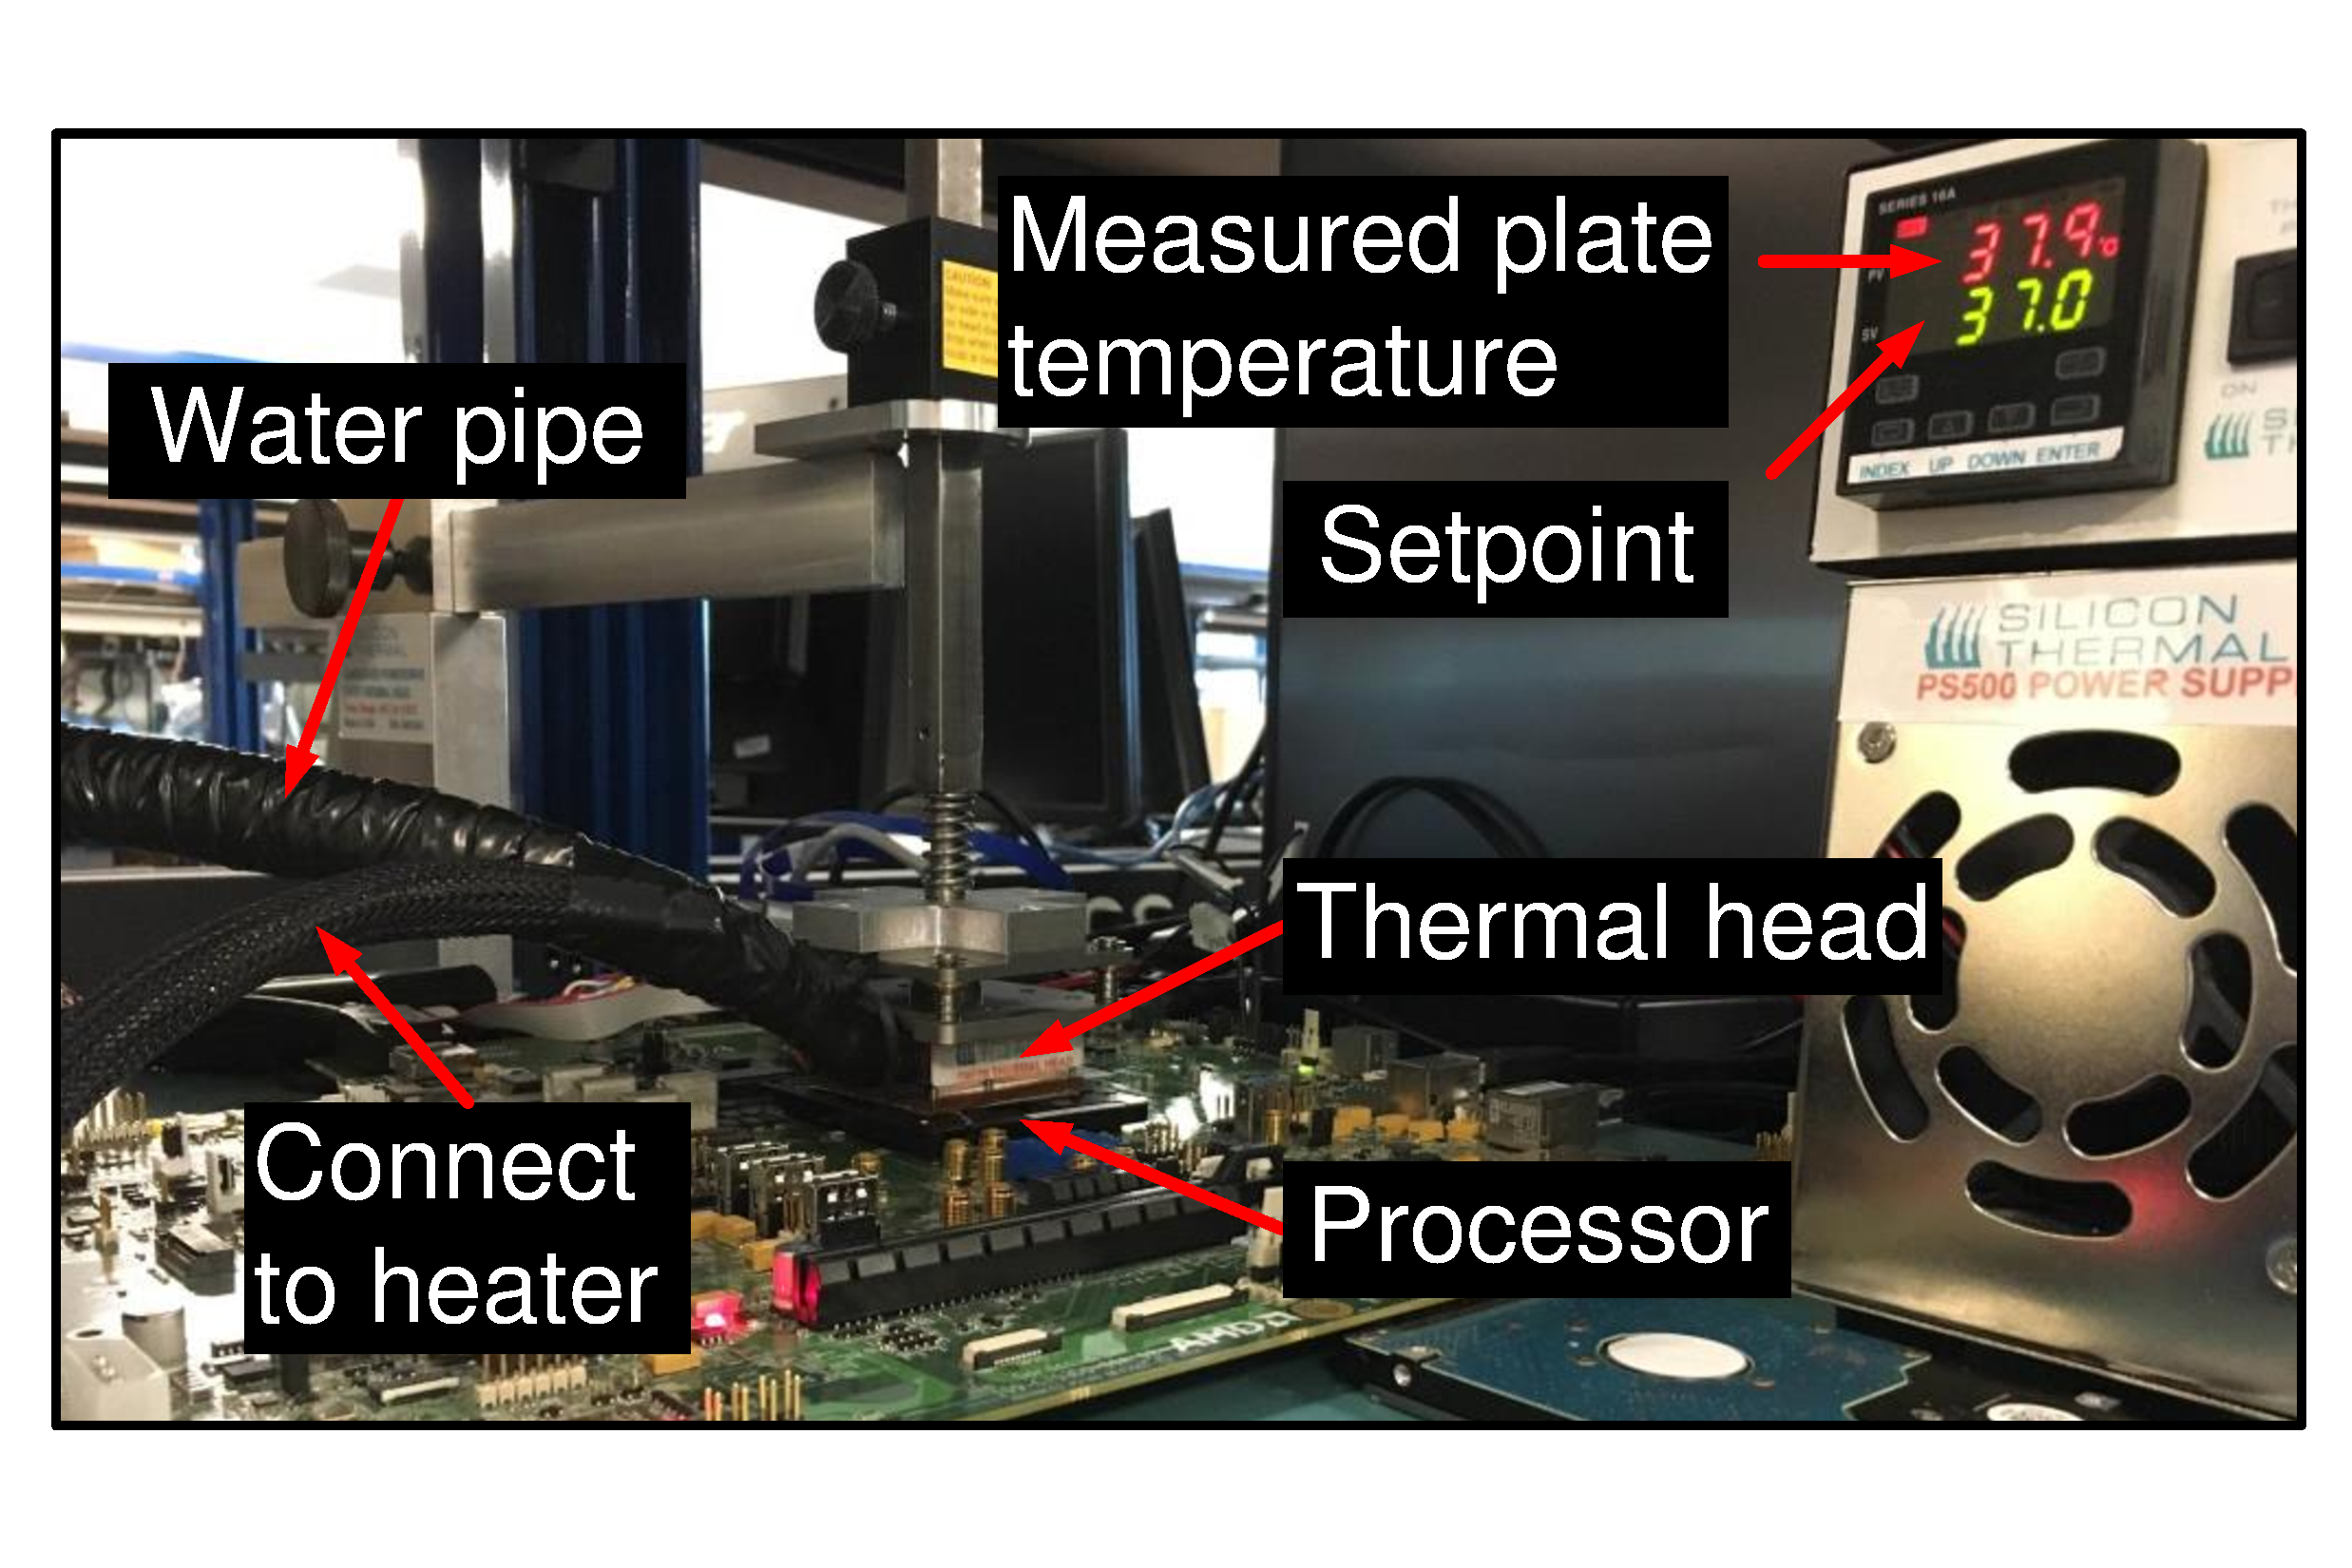
\includegraphics[trim=0 55 0 55,clip,height=1.5in]{graphs/temperature/temperature-control.pdf}
                \caption{Temperature control setup.}
                \label{fig:temp-control-photo}
  \end{minipage}

\end{figure}

\subsection{AMD\textsuperscript{\textregistered} A10-8700P Accelerated Processing Unit}
\label{sec:temperature:setup:apu}

The AMD\textsuperscript{\textregistered} A10-8700P Accelerated Processing Unit (APU) is a System-on-Chip manufactured in 28 nm HKMG planar bulk technology. It integrates two CPU core-pairs, eight GPU cores, and other components as shown in~\Fig{fig:die-shot}. Each CPU core-pair contains two out-of-order cores that share the front-end and floating point units. Each GPU core includes four 16-lane wide single instruction multiple data (SIMD) units. 

We conducted temperature inversion studies on both the CPU and GPU. A separate power delivery network allows us to control the CPU and GPU voltage independently. But in this work, we present the results for the GPU only because the GPU's throughput-oriented architecture allows low-voltage region operation with meaningful and realistic performance. However, because the temperature inversion effect we study depends solely on the supply voltage, and not necessarily the underlying architecture, the analysis and benefits we present on the GPU naturally do extend to the CPU as well.

The GPU clock is set at 300 MHz in the voltage region we explore around 0.7~V. We pick 300MHz because its associated low voltage is within the temperature inversion region, and makes it possible to explore the potential impact of temperature inversion on future near-threshold technologies. The 300 MHz frequency corresponds to the GPU's lowest P-State, and in practice, we have observed this P-State being exercised frequently during normal workload execution. 

We use the ATITool~\cite{atitool} to set the GPU's voltage and frequency over a wide operating range. To measure power, we use a National Instrument's DAQ that reads the GPU's isolated supply voltage rail once every 10~ms.

\subsection{Temperature Control Setup}
\label{sec:temperature:setup:temp}

To characterize temperature inversion's effect on performance and power under different operating conditions, we have to carefully regulate the processor's on-die temperature. In our work, we generally sweep temperature range from 0\C to 80\C. This temperature range falls within the product's operating temperature range and does not affect aging significantly.

\Fig{fig:temp-control-photo} shows our temperature control setup. A thermal head is attached to the processor package. To stabilize the die temperature, which is measured via an on-chip thermal diode, at a user-specified target value, the thermal head's temperature is adjusted every 10~ms. Physically, the thermal head's temperature is controlled via a water pipe and a heater. The water pipe is connected to an external chiller to offer low temperatures while the heater increases temperature to reach the desired temperature setting. Under feedback control, we see a 2\C temperature variation on the diode in the worst-case. So, for instance, \Fig{fig:temp-control-photo} shows the thermal head sets its temperature to 37\C to let the die temperature stay at 40\C. 

\subsection{Timing Margin Sensors: On-chip Power Supply Monitors (PSMs)}
\label{sec:temperature:setup:psm}

We use power supply monitors (PSMs)~\cite{grenat20145,gillespie2014streamroller} to accurately measure circuit speed changes in the chip under different temperature conditions. A PSM is a time-to-digital converter that reflects circuit time-delay or speed in numeric form. Originally designed as a voltage noise sensor, a PSM can sense minute circuit timing changes due to $di/dt$ droops~\cite{grenat20145}. We use the PSM as a means to characterize circuit performance under temperature variation.

\begin{figure}[h]
    \centering
    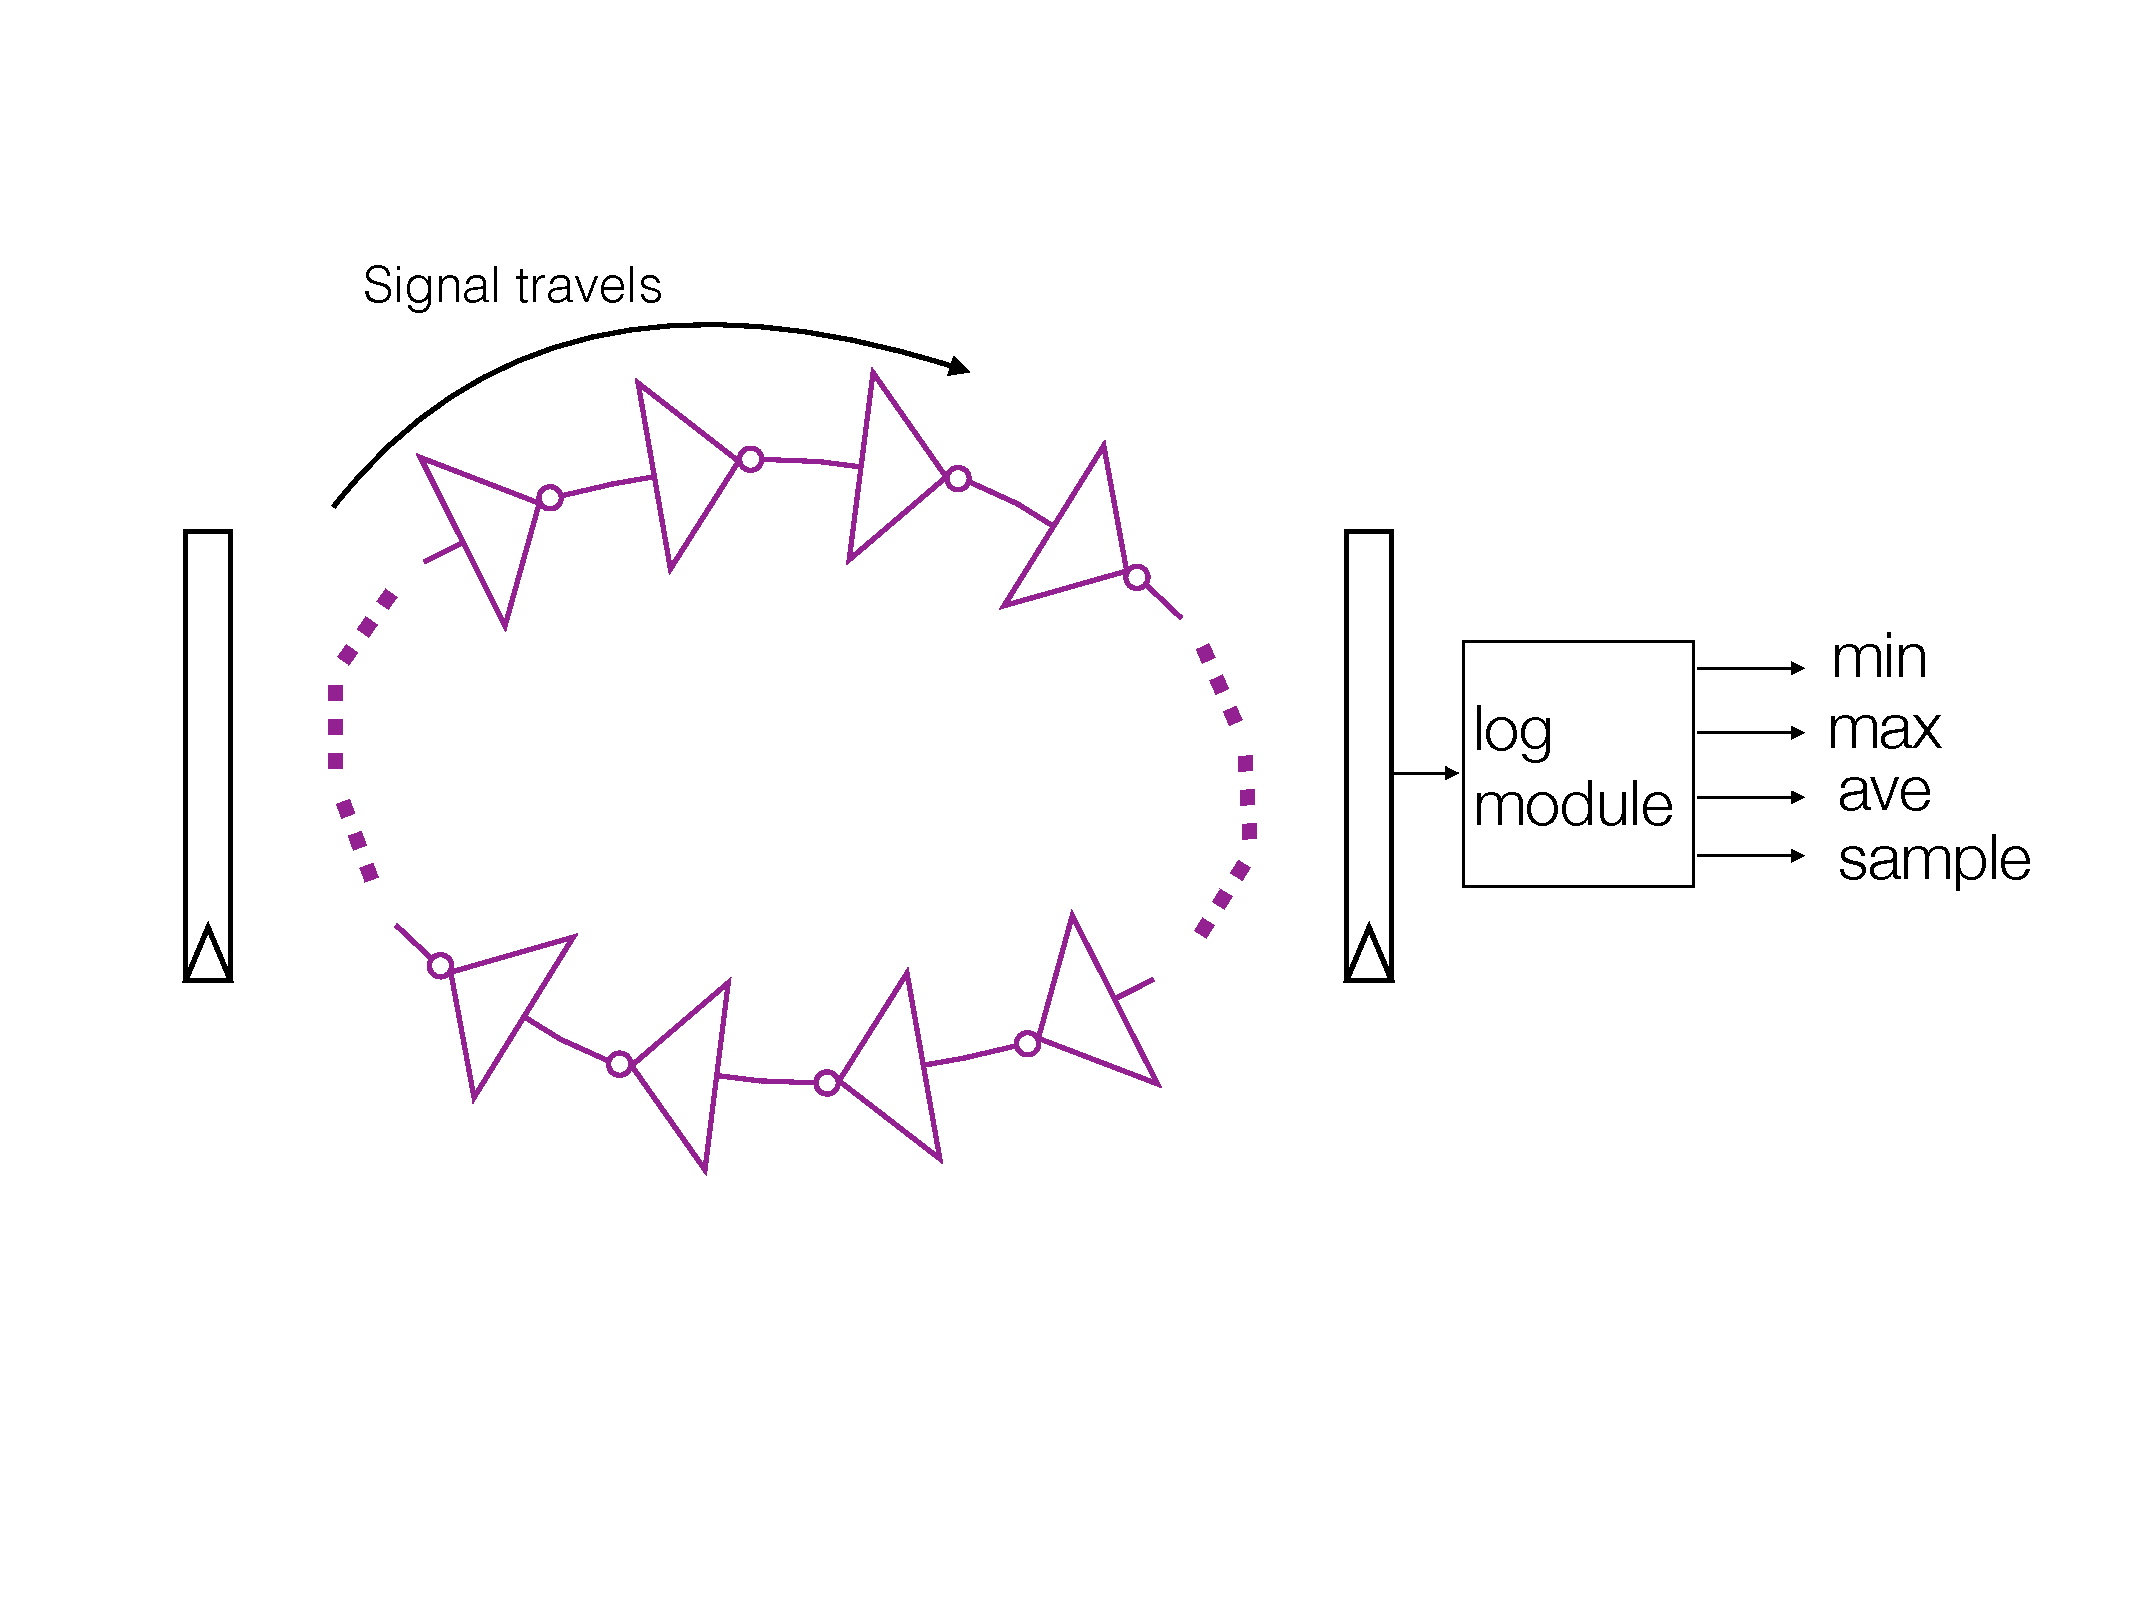
\includegraphics[trim=40 150 40 150,clip,width=0.8\columnwidth]{graphs/temperature/psm.pdf}
    \caption{Power supply monitors (PSMs) measures pipeline speed/timing margin with an inverter ring. By counting how many inverters an edge has traveled through, the PSM reports a digital value that reflects circuit speed.}
    \label{fig:psm-struct}
\end{figure}

\Fig{fig:psm-struct} shows the structure of a PSM. Its core component is a ring oscillator that counts the number of inverters an ``edge'' has traveled through in each clock cycle. When the circuit is faster (e.g., under smaller $di/dt$ effects or stronger temperature inversion), an edge can pass more inverters and PSM will produce a higher count output. A supporting module logs ring oscillator's per-cycle output and accumulates the minimum, maximum, and average values over a time.

The A10-8700P processor has ten PSMs in each CPU core-pair and two PSMs in each GPU core, distributed across the cores to account for process variation and spatial differences in $di/dt$ effect. Through measurements we determined that the changes in the different PSM readings under different temperatures are nearly identical, thus we only show the result of one representative PSM in GPU. The results are representative of using other or more than one PSM. 

For reasons that prevent us from showing absolute values, we normalize the PSM reading to a reference value measured under 0.7~V, 300~MHz, 0\C, and idle chip condition. We log the minimum, maximum, and average output of all the PSMs. 

\section{Characterizing Timing Margin Under Temperature Inversion Variation}
\label{sec:temperature:characterize}

In this section, we first view the timing margin sensor (i.e., PSM) as a normal logic path to understand circuit performance under different temperature environment (\Sec{sec:temperature:characterize:psm}). Then, we use the circuit speed difference to extrapolate how much extra margin can be squeezed out due to timing margin change caused by temperature inversion variation (\Sec{sec:temperature:characterize:extrapolate}).

\subsection{Circuit Speed Variation Under Different Temperature}
\label{sec:temperature:characterize:psm}

The PSM by itself is a digital circuit located between the pipeline latches with other normal logic paths~\cite{sriram2016avfs}, and therefore its speed characteristics are representative of a pipeline's overall performance. For this reason, we use the PSM's output to quantify circuit performance across a wide range of different steady-state temperatures. 

\begin{figure}
\centering
    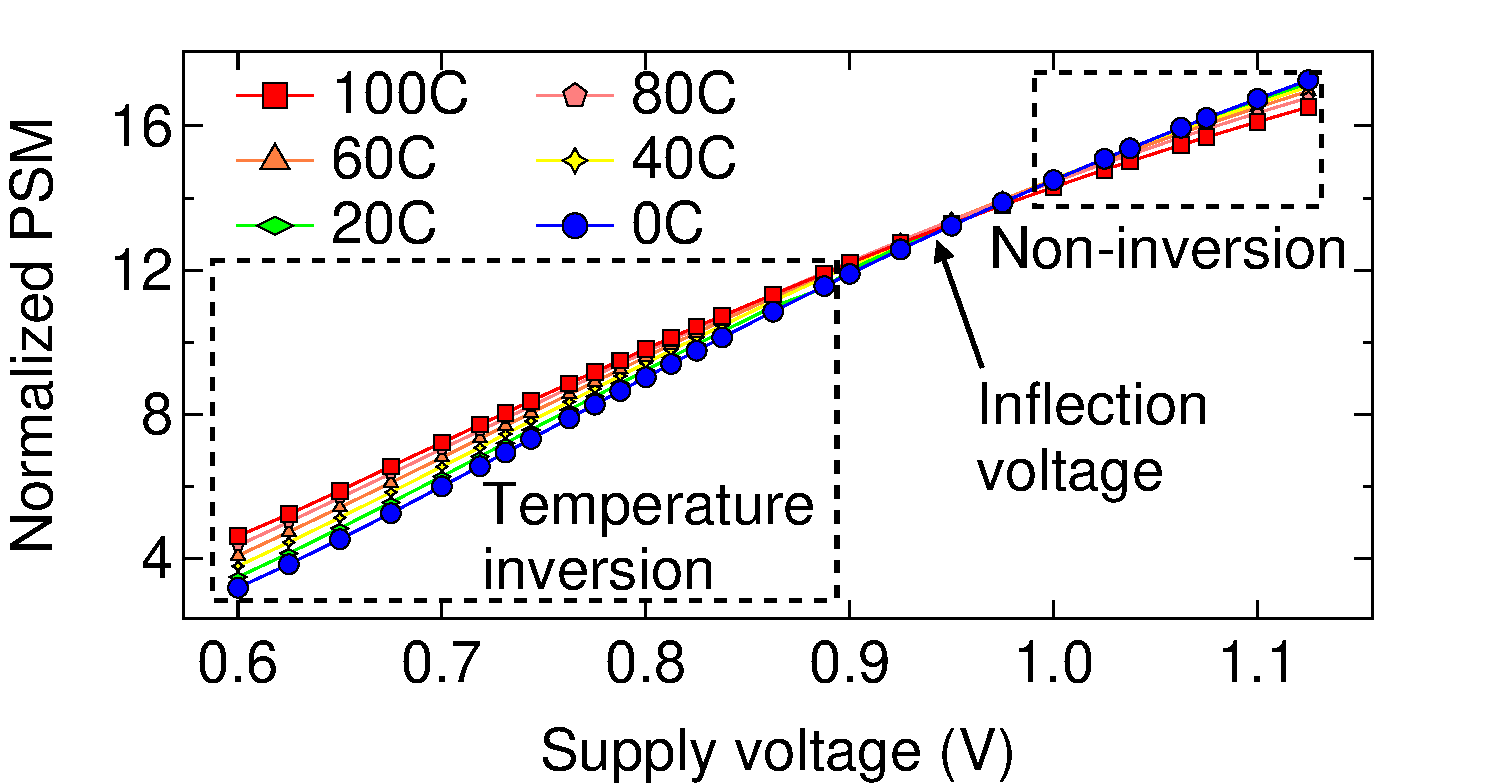
\includegraphics[trim=0 0 50 20,clip,width=.9\linewidth]{graphs/temperature/idle-psm-volt-temp.pdf}
    \caption{Temperature inversion happens below 0.9~V and is progressively stronger when voltage scales down.}
    \label{fig:psm-wide-range}
\end{figure}

We keep the chip idle (i.e., the clock is still running) and read the PSM's ``average'' value to exclude the $di/dt$ effect caused by workload dynamics. \Fig{fig:psm-wide-range} shows the circuit speed under different supply voltages and die temperatures. Speed is reflected by the PSM's normalized output -- higher value implies a faster circuit. At a higher supply voltage, the circuit switches faster, and the PSM can travel more inverters in a cycle which produces a higher count. The voltage-to-PSM relationship conforms to similar analysis as in~\cite{zu2015adaptive}.

We find that temperature's impact on circuit performance depends on the supply voltage. In the high supply voltage region around 1.1 V, the PSM's reading becomes progressively smaller as the temperature rises from 0\C to 100\C. The circuit is operating slower at a higher temperature, which aligns with conventional belief~\cite{leng2015safe}. The reason for this circuit performance degradation is that the transistor's carrier mobility decreases at a higher temperature, leading to smaller switch-on current ($I_{on}$) and longer switch time~\cite{wolpert2012temperature}.

Under a lower supply voltage, the PSM's reading increase with higher temperature, which means the circuit switches faster (i.e., the temperature inversion phenomenon). Under temperature inversion the transistor's threshold voltage ($V_{th}$) decreases linearly as temperature increases~\cite{wolpert2012temperature,park1995reversal,dasdan2006handling}. Thus, for the same supply voltage, a lower $V_{th}$ provides more drive current ($I_{on}$) which makes the circuit switch faster. The speedup effect is more dominant when the supply voltage is low because then the supply voltage is closer to $V_{th}$.

When the supply voltage is low enough, the speedup contribution from the reduced $V_{th}$, at some point, will balance out the carrier mobility slowdown. We call this voltage point the {\it inflection voltage}. The inflection voltage may change from chip to chip due to $V_{th}$ variations, and it can be characterized during the binning process. In~\Fig{fig:psm-wide-range}, we show that the tested processor's inflection voltage is between 0.9~V and 1~V. In this region, the temperature does not have a notable impact on circuit performance. Below the inflection voltage (0.95~V) is the temperature inversion region while above it is the non-inversion region. Half of the GPU's P-states, which range from 0.75~V to 1.1~V, operate in the temperature inversion region.

In~\Fig{fig:psm-wide-range}'s temperature inversion region, the speed change between any two temperatures increases when the supply voltage scales further away from the inflection point. As voltage scales into the lower voltage region around 0.6~V, the PSM reading varies by more than 40\%, indicating the drastic speedup at a higher temperature. As voltage goes lower towards the near-threshold region, the overdrive voltage ($V_{dd}-V_{th}$) becomes small and it is very sensitive to small $V_{th}$ changes. Thus, temperature inversion's $V_{th}$ reduction has a more significant impact on device performance.

\begin{figure}
    \centering
    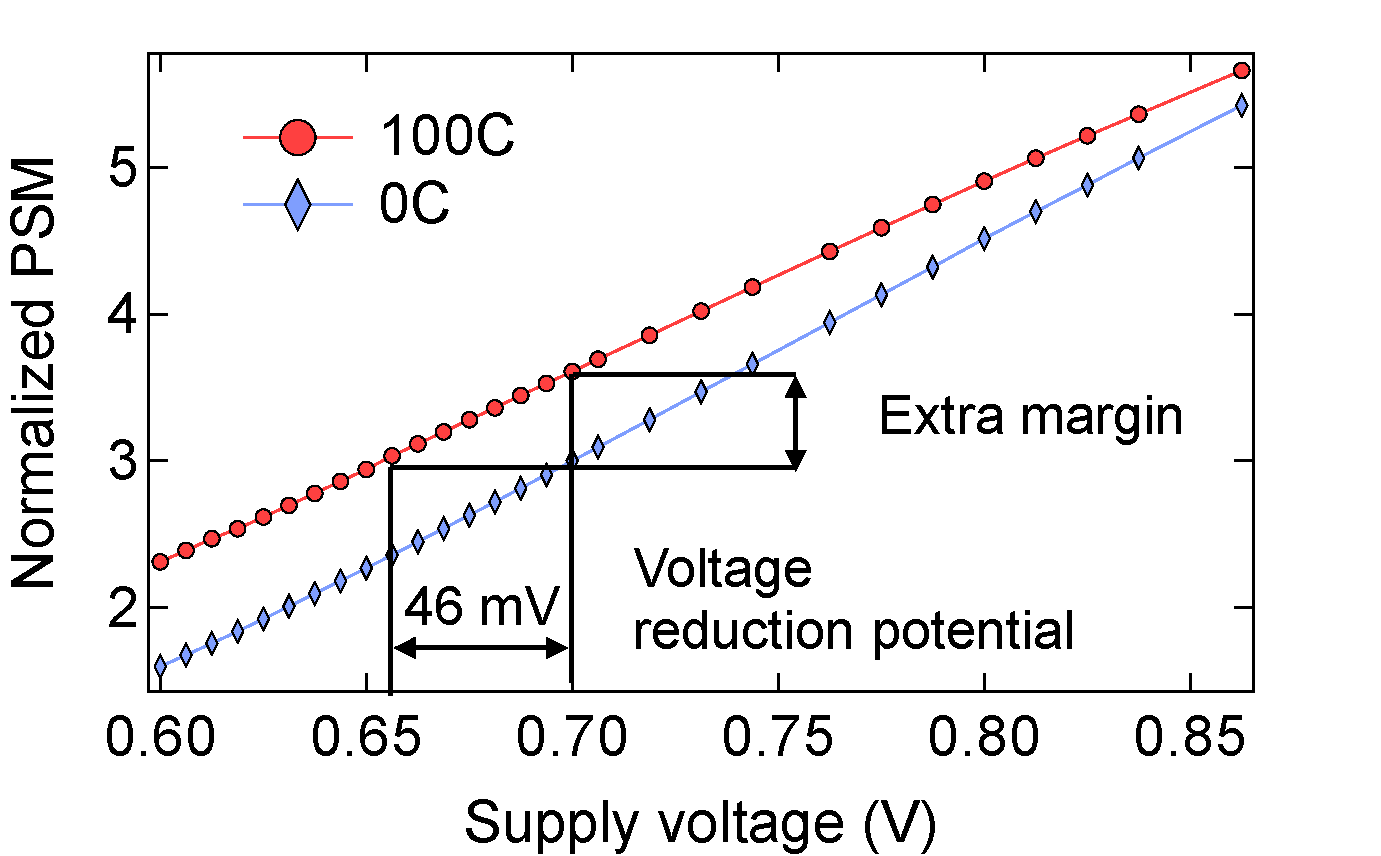
\includegraphics[trim=0 0 50 20,clip,width=.8\linewidth]{graphs/temperature/idle-psm-volt-nt.pdf}
    \caption{Estimating voltage reduction potential based on PSM characterization at different temperatures.}
    \label{fig:psm-nt}  
\end{figure}

\Fig{fig:psm-nt} zooms into the low voltage region between 0.6~V and 0.86~V and has a clearer view of temperature inversion. The figure shows temperature inversion's performance benefit at 100\C over the 0\C baseline, and this benefit increases as the supply voltage decreases. Hereon forward we use temperature inversion at 0.7~V as a case study to dive deeper and get more insights. Although we restrict ourselves to this single voltage, there is ample opportunity to demonstrate how temperature inversion may add new ingredients to overall system management.

\subsection{Estimating Active Timing Margin's Undervolting Opportunity}
\label{sec:temperature:characterize:extrapolate}

In this subsection, we provide a ``design space exploration'' of active timing margin's voltage reduction opportunity. When running workloads, chip temperature frequently goes up and speeds up circuits because of temperature inversion. This adds extra timing margin in the pipeline, and the extra margin can be exploited via undervolting. 

To determine the amount of extra timing margin that can be exploited, we first need a ``baseline margin'' where timing margin is not overprovisioned for temperature variation. In other words, the ``baseline margin'' is the timing margin allocated for the worst-case temperature. It can tolerate all other effects such as $di/dt$ and aging at worst-case temperature, yet circuit speed cannot be degraded anymore compared to worst-case temperature. When undervolting, it is crucial that the system only reclaims the extra timing margin added from this ``baseline margin'' and does not reclaims anymore. Otherwise, pipeline timing may fail under some worst-case workloads, such as in the case of voltage stressmarks~\cite{kim2012audit,bertran2014voltage}. 

We use the timing margin measured at 0\C as the ``golden'' reference when reclaiming temperature inversion's extra margin. In other words, the timing margin delivered by our active timing margin scheme should match the ``golden'' reference. Under this constraint, we can undervolt to maximize power saving. 

We choose 0\C as the reference because under temperature inversion lower temperature degrades circuit performance. Even though 0\C rarely occurs in desktop, mobile, and datacenter applications, the timing margin still needs to be set to tolerate this worst-case condition. In the industry, 0\C or below is used as a standard circuit design guideline~\cite{altera2010timing}. In certain scenarios, such as military use, an even more conservative reference of -25\C is considered~\cite{dasdan2006handling}.

\Fig{fig:psm-nt} shows our estimation process of how much voltage can be reduced via active timing margin. The PSM difference between the high-temperature 100\C line and the ``golden reference'' line at 0\C represents the extra timing margin in the units of inverter delays. In other words, it reflects how much faster the circuits can run at a higher temperature. To bring the faster circuit back to the original speed, supply voltage needs to reduce such that under a higher temperature the PSM will ideally read the same value.

\begin{figure}
  \centering
  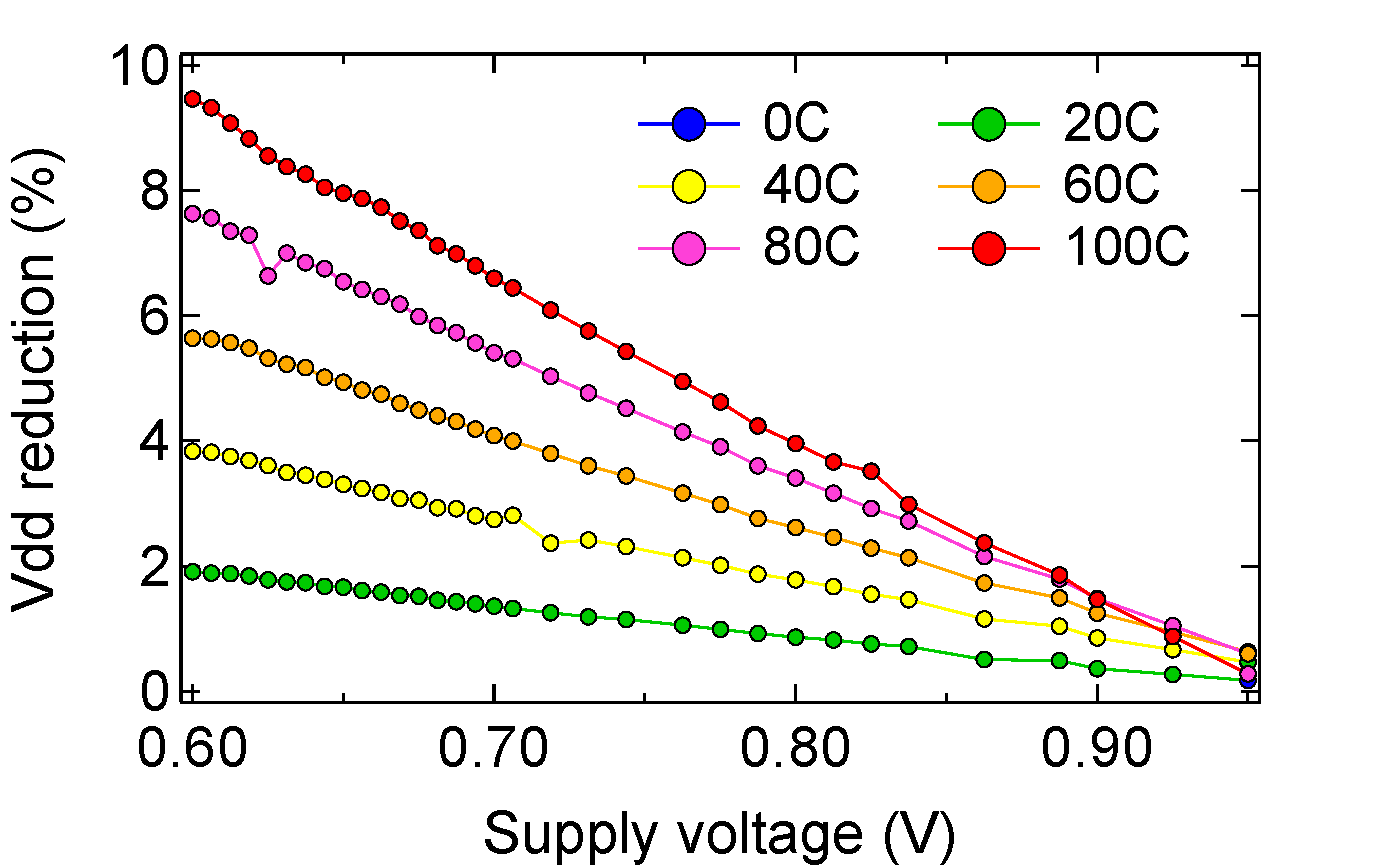
\includegraphics[trim=0 0 50 20,clip,width=.8\linewidth]{graphs/temperature/extrapolate-uv-potential.pdf}
  \caption{Voltage reduction potential is more pronounced in the near-threshold low voltage region.}
  \label{fig:uv-potential} 
\end{figure}

We estimate the voltage reduction potential with linear extrapolation.~\Fig{fig:uv-potential} shows the estimated opportunity at different temperatures. As supply voltage scales down, the voltage reduction potential goes up almost linearly. Temperature inversion effect is stronger in the lower voltage regions, and hence the greater timing margin opportunity. At 0.6~V and 100\C, the extra timing margin provided by temperature inversion can turn into almost 10\% voltage reduction compared to 0\C. As a reference, 5\% voltage reduction is considered significant in previous works~\cite{webel2015robust}. At 0.7~V in our study, we can have 1.5\% to 7\% voltage reduction potential depending on the processor temperature.


\section{Temperature Inversion States (Ti-States)}
\label{sec:temperature:tistate}

Having understood temperature inversion's potential for active timing margin, we propose a systematic method to establish a precise and reliable temperature to voltage mapping that implements active timing margin. The temperature to voltage mapping is discrete as voltage regulator module's output voltage is quantized in small steps~\cite{intelVRM}. The final mapping is, therefore, in a table format, which we call \tistates. Similar to the way P-states functions for DVFS, \tistate is a natural evolution of power management mechanisms for active timing margin.

\subsection{Methodology to Construct the Ti-States Table}
\label{sec:temperature:temperature:construct}

We propose a workload-centric methodology that constructs a set of temperature-voltage states in the inversion region (\tistates) at test-time. A workload-centric approach ensures \tistates will work in the face of workload-induced uncertainties like $di/dt$ and IR effects. We use a subset of workloads as the ``training'' set to first get a tentative temperature-voltage mapping. Then we validate this mapping with another set of ``test'' workloads to establish the final \tistate. During training the \tistate is constructed in a manner that is agnostic to workload-specific settings, so we can be sure our voltage selection will provide enough margin for any workload that is run on the processor.

For each of the training workloads, we first measure their ``golden'' reference margin at 0\C under our controlled temperature setup. Then, at the temperature being characterized, we select four candidate voltages. These candidate voltage are picked such that they are around the extrapolated voltage value from~\Fig{fig:uv-potential}. The candidates voltages are chosen such that they are two VRM steps above and two VRM steps below the extrapolated value. 

\begin{algorithm}[h]
\caption{\tistate Construction Methodology}
\label{train-algo}
\begin{algorithmic}[1]
\Procedure{Get Reference Margin}{}
\State $\text{set voltage and temperature to reference}$ 

\For{each training workload} 
\State $\textit{workloadMargin} \gets \text{PSM measurement}$
\State $\text{push } \textit{RefMarginArr}\text{, }\textit{workloadMargin}$ 
\EndFor
\Return \textit{RefMarginArr}
\EndProcedure

\Procedure{Explore Undervolt}{}
\State $\textit{initVdd} \gets \text{idle PSM extrapolation}$ 
\State $\textit{candidateVddArr} \gets \text{voltage around }\textit{initVdd}$
\State $\textit{minErr} \gets \text{MaxInt}$ 
\State $\text{set exploration temperature}$

\For{each \textit{Vdd} in \textit{candidateVddArr}} 
\State $\text{set voltage to } \textit{Vdd}$

\For{each training workload} 
\State $\textit{workloadMargin} \gets \text{PSM measurement}$
\State $\text{push } \textit{TrainMarginArr}\text{, }\textit{workloadMargin}$ 
\EndFor

\State $\textit{err} \gets \text{diff(}\textit{RefMarginArr}\text{,}\textit{TrainMarginArr}\text{)}$
\If {$\textit{err} < \textit{minErr}$} 
\State $\textit{minErr} \gets \textit{err}$
\State $\textit{exploreVdd} \gets \textit{Vdd}$
\EndIf
\EndFor
\Return \textit{exploreVdd}
\EndProcedure

\end{algorithmic}
\end{algorithm}

Once we have the set of candidate voltages, we step through each candidate voltage and record the training workloads' timing margin using the PSM at every temperature that is being characterized. The timing margin measured at the candidate voltage is compared against the reference margin. Finally, we select the candidate voltage that has the minimum PSM difference from the golden reference. 

It is worthwhile to note that on our particular chip the data variation for the 16 PSMs on our GPU is under 2\%, so it makes little difference to use worst-case versus average. However, under severe intra-chip variation, transistor's undervolting potential can differ significantly. In that case, worst-case PSMs values need to be used for comparison.

\begin{figure}[t]
    \centering
    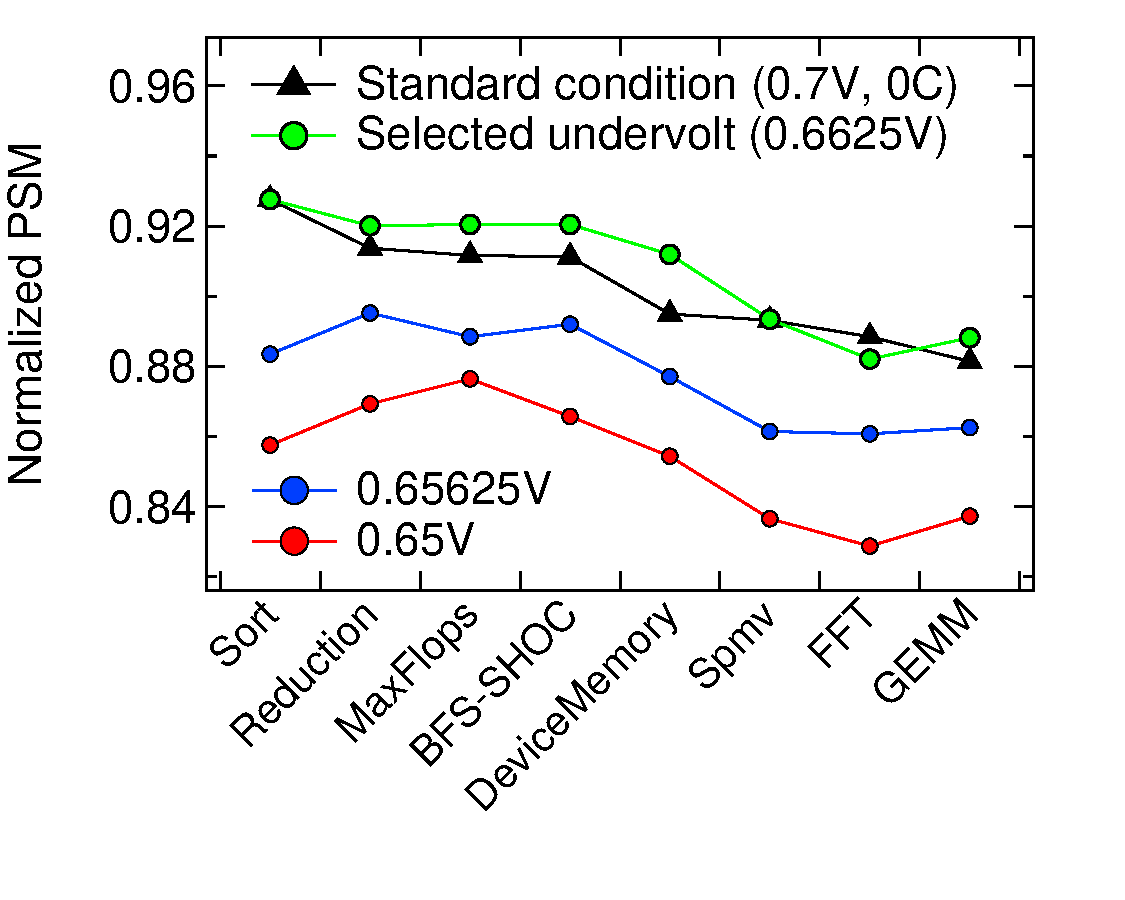
\includegraphics[trim=-30 0 0 0,clip, width=0.7\linewidth]{graphs/temperature/explore-uv-shoc.pdf}
    \caption{Exploring \tistate at 80\C: we measure the ``training'' workloads' timing margin, and choose the $V_{dd}$ that best tracks the standard margin.}
    \label{fig:train-uv}
\end{figure}

\Algo{train-algo} summarizes our methodology. \Fig{fig:train-uv} shows an example at 80\C. At this temperature, \Fig{fig:uv-potential}'s extrapolated voltage is 0.65625 V. The candidate voltages are 0.6625~V, 0.65625~V, and 0.65~V. Our platform's smallest VRM step is 6.25mV. The original four candidate voltage is capped by a lower hard limit of 0.65~V, and so we cannot set the voltage any lower. \Algo{train-algo} chooses 0.6625 V as the \tistate voltage for 80\C because it has the closest timing margin compared to ``golden'' reference. Other candidate voltages with less timing margin run the risk of hampering the timing safety under potentially worst-case workloads.

\begin{figure}[t]
  \centering
      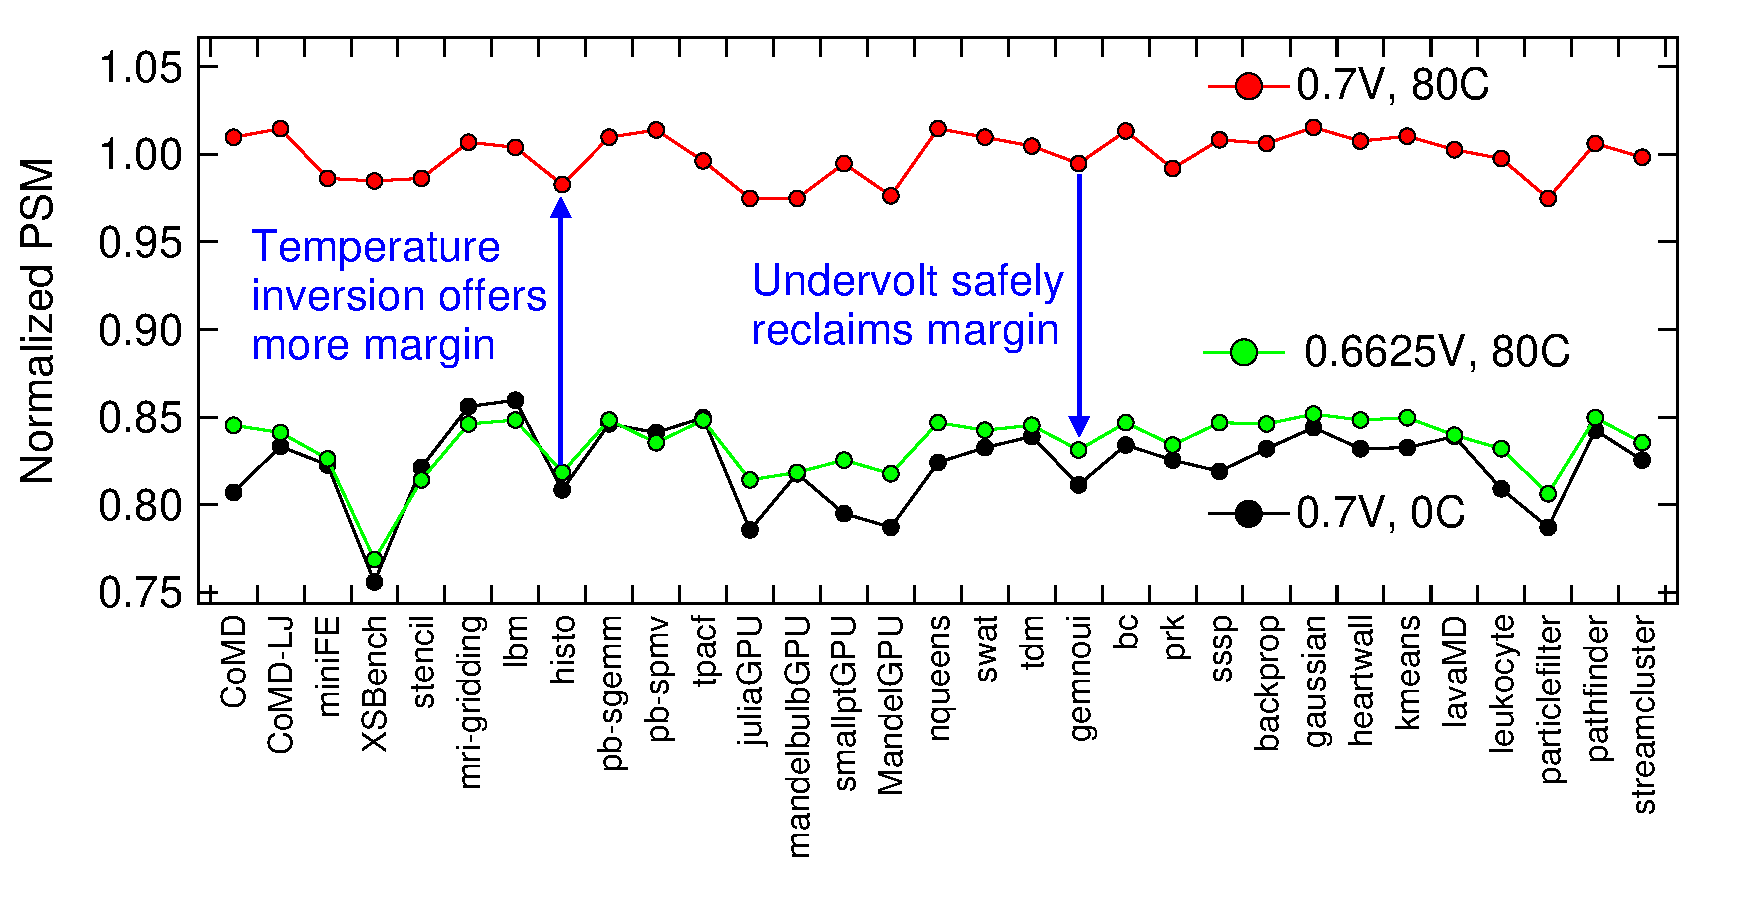
\includegraphics[trim=0 20 30 15,clip,width=\linewidth]{graphs/temperature/validate-uv.pdf}
      \caption{\tistate undervolting decision at 80\C closely tracks the ``golden'' reference runs' timing margin, which is needed for reliability.}
      \label{fig:validate-uv}
\end{figure}

\Fig{fig:validate-uv} verifies \Algo{train-algo}'s \tistate selection at 80\C. At 0.7~V, going from 0\C to 80\C offers more than 15\% extra timing margin. After voltage reduction, the workload timing margins closely track the golden reference with some workloads showing slightly higher margin.

\Fig{fig:validate-uv} proves yet another important point. It shows that the voltage explored using a small set of training workloads can be safely applied to future unknown workloads. The reason that the approach we present works in practice is because the extra margin that arises from temperature inversion is mainly a device property and it is workload-independent.

\subsection{Evaluating Ti-State's Voltage and Power Reduction Effects}
\label{sec:temperature:temperature:table}

\Algo{train-algo} will repeat the same process at different temperatures. Using results similar to~\Fig{fig:train-uv} and \Fig{fig:validate-uv}, our methodology will eventually construct a temperate-voltage pairing table with all the proper \tistates.~\Tab{table:explore-err} shows the measured results on our A10-8700P processor for 20\C, 40\C, 60\C, and 80\C. For each temperature, there is one voltage that has the smallest deviation from the ``golden'' reference margin, as highlighted and bolded in the table. These points are selected as the final \tistates for the processor to use.

\begin{table}
\centering
\resizebox{0.75\textwidth}{!}{
	\begin{tabular}{ l | c | c | c | c | c }
    \Xhline{3\arrayrulewidth}
     & {\bf20\C}  & {\bf40\C}  & {\bf60\C}  & {\bf80\C}  & {\bf100\C} \\[1.4ex] \Xhline{3\arrayrulewidth}
    {\bf693.75mV}   &   3.7\% & - & - & - & -  \\
    {\bf687.50mV}   &   \cellcolor{blue!25}{\bf \color{black}2.2\%} &  - & - & - & -  \\
    {\bf681.25mV}   &   8.4\% & \cellcolor{blue!25}{\bf \color{black}2.3\%}  & - & - & -  \\
    {\bf675.00mV}   &   13.9\% & 5.3\% & 4.9\% & - & -  \\
    {\bf668.75mV}   &   - & 9.5\% & \cellcolor{blue!25}{\bf \color{black}2.5\%} &  - & -  \\
    {\bf662.50mV}   &   - & 13.5\% & 6.5\% & \cellcolor{blue!25}{\bf \color{black}1.9\%}  & -  \\
    {\bf656.25mV}   &   - & - & 12.2\% & 5.6\% & 9.9\%  \\
    {\bf650.00mV}   &   - & - & - & 9.3\% & \cellcolor{blue!25}{\bf \color{black}5.1\%}   \\
    \Xhline{3\arrayrulewidth}
  \end{tabular}
}
\vspace{0.2cm}
\caption{PSM error compared to the reference setting for different $<temperature, voltage>$ configurations.}
\label{table:explore-err} 
\end{table}

\tistate table construction would add little overhead to existing silicon test procedures. Per-bin or even per-part characterization is already an industry-standard practice, especially for the high-end server market sector. Therefore, we believe that \tistate table construction is a practical approach.

At runtime, the power management scheme can use temperature sensor data to index into a \tistate table and determine a suitable supply voltage~\cite{sriram2016avfs}. In our work and the restricted scope of this paper, \tistates are constructed for the GPU clock frequency of 300~MHz. In practice, however, the \tistate table can be constructed across different frequencies, and the power management unit can index into the right table by frequency during runtime. 

\begin{figure}[t]
  \centering
  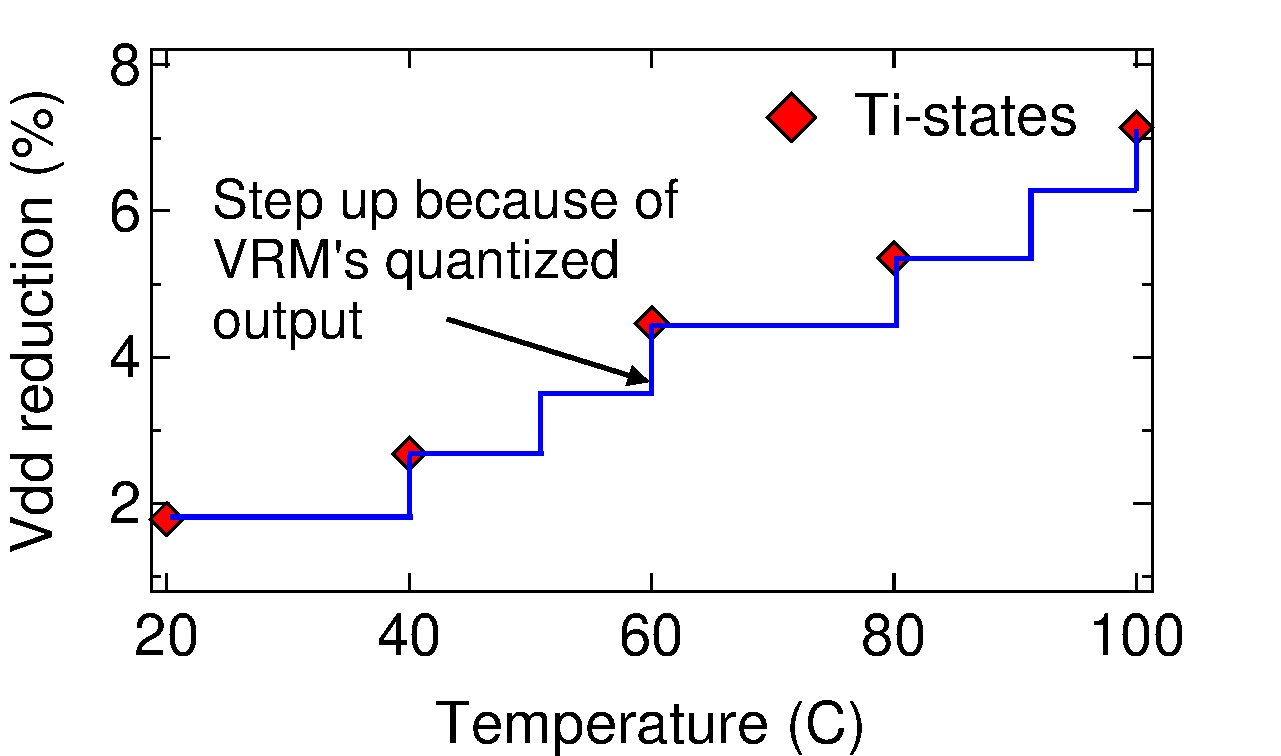
\includegraphics[trim=0 -10 0 0,clip,width=0.7\linewidth]{graphs/temperature/explore-extrapolate.pdf}
  \captionof{figure}{$V_{dd}$ reduction due to \tistates. The line corresponds to the VRM's quantized output values.}
  \label{fig:tistate-show}
\end{figure}

We use a representative subset of all workloads to evaluate \tistate's power reduction at different temperatures. We start with \Fig{fig:tistate-show}, which shows the $V_{dd}$ reduction at various \tistates. One temperature range corresponds to one voltage and this is because of the VRM's quantized output. To make the VRM reduce voltage by one step, the temperature has to be high enough to speed up the circuit beyond the current point. Between 20\C and 40\C, the VRM can reduce $V_{dd}$ by exactly one step, yet from 40\C to 60\C there are two VRM steps in between. The results show that $V_{dd}$ reduction is larger at a higher temperature because the extra timing margin offered by temperature inversion is larger than at a lower temperature. 

\begin{sidewaysfigure}
  \centering
  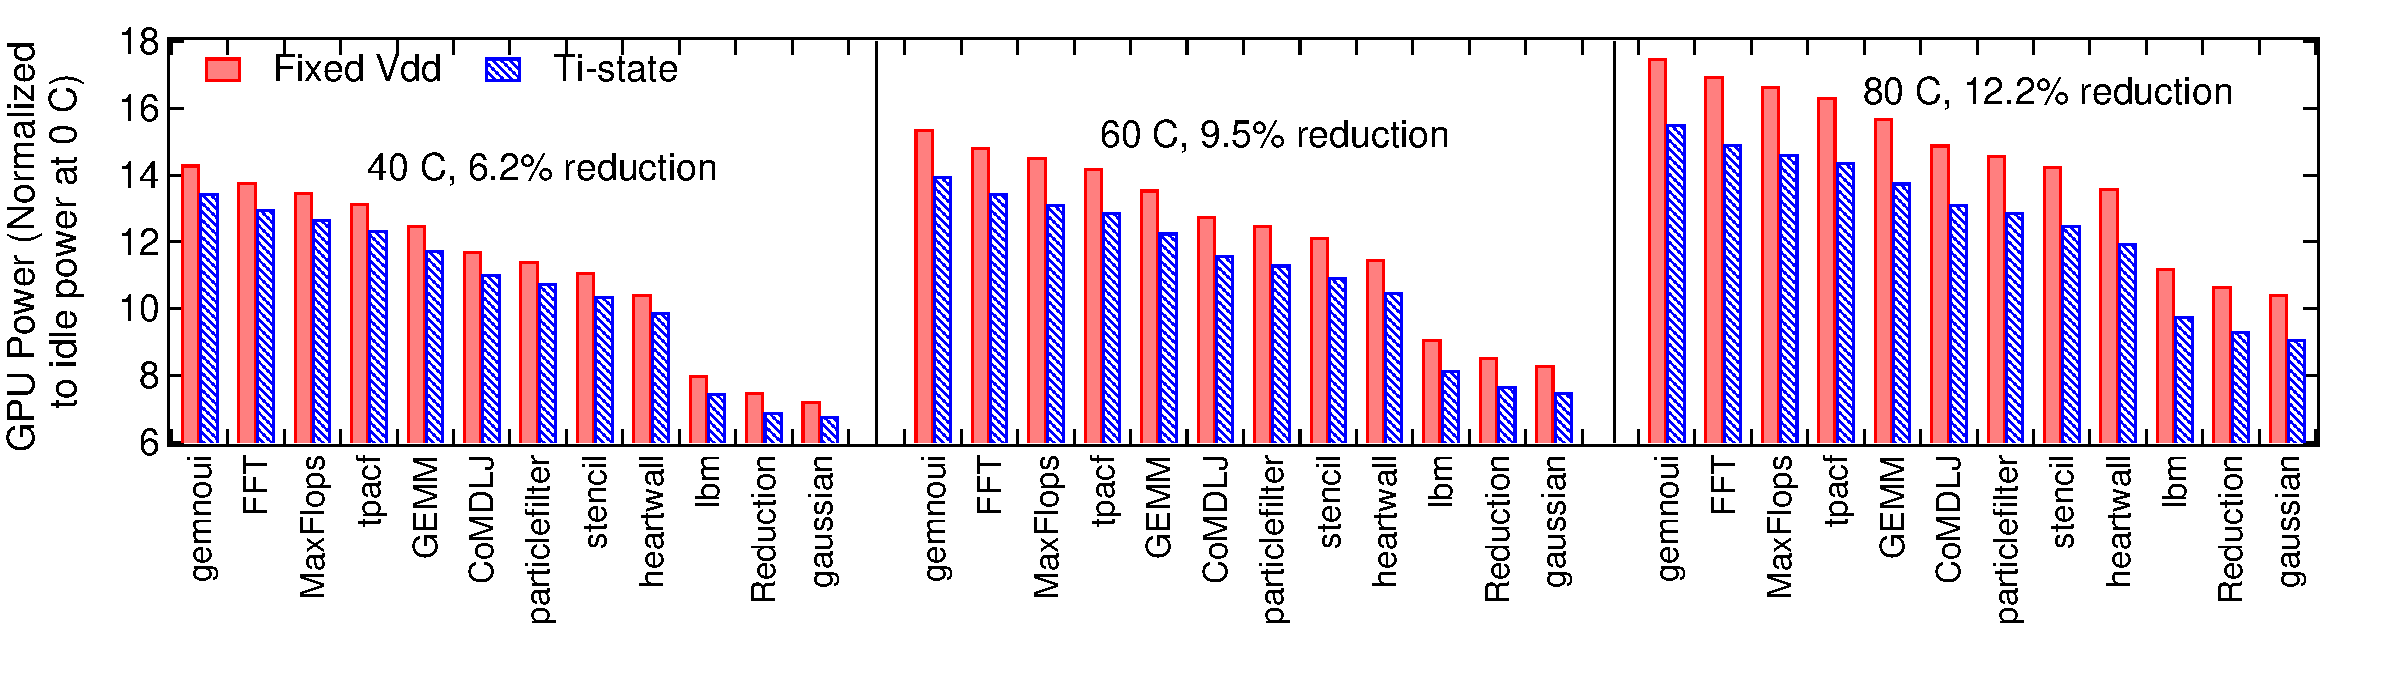
\includegraphics[trim=0 0 0 0,clip,width=\linewidth]{graphs/temperature/evaluate-tistate.pdf}
  \caption{Power saving increases at higher temperatures. We mimic workload temperature by externally controlling die temperature to a 40\C~--~80\C range. \tistate's power reduction is independent of the workload activity. }
  \label{fig:power-save-orig}
\end{sidewaysfigure}

In~\Fig{fig:power-save-orig} we compare the average power savings of the various GPU workloads as a result of the $V_{dd}$ reduction at different temperatures. We set the die temperature manually using our temperature control setup to 40\C, 60\C, and 80\C to mimic the various temperature conditions that the processor typically faces. We manually set the temperature because the GPU on the A10-8700P does not heat up the chip often in the voltage region we study, which limits the temperature range we can use to thoroughly characterize. Therefore, rather than examine the workloads under a ``free run,'' we interject with external temperature control. But on the more high-end and power-hungry server parts, the GPU would hit the higher temperatures we are characterizing.

An added benefit of temperature control is that it facilitates controlled and repeatable experiments. Our choice of temperatures is reasonable because, usually, for a high-end cooling system that has around 0.2\C/W ambient-silicon thermal resistance, a workload consuming 60 W will have a steady state temperature of 40\C. For a less capable 0.5\C/W cooling system the same workload will stabilize around 60\C~\cite{skadron2004temperature,huang2006hotspot,fan2016computational}. So we cover different cooling options.

\Fig{fig:power-save-orig} shows that on average the \tistates can save 6.2\%, 9.5\%, 12.2\% power at 40\C, 60\C and 80\C, respectively. The power saving primarily comes from dynamic power reduction. Leakage power consumption also reduces at lower voltages, but only by a little. At each temperature, the relative power saving does not vary much between different workloads, but this is to be expected because \tistate's voltage reduction is workload independent. Hence, the relative dynamic power saving for each workload should stay the same for each temperature. In practice, different workloads stabilize at different temperatures at runtime, and \tistate will reduce the operating voltage accordingly. When the temperature varies under workload phase changes, a VRM can index into \tistate table in real-time and adjust the supply voltage step by step~\cite{sriram2016avfs}.


\section{Managing Ti-State Processors in Advanced Technology Nodes}
\label{sec:temperature:manage}

In this section, we compare and contrast the benefits of \tistate's power savings on traditional planar bulk CMOS versus the more recent FinFET and FD-SOI process technologies. FinFET is already present in latest processors~\cite{intel22nm,samsung14nm} at the time of this proposal, and both technologies will be more broadly adopted in the coming years~\cite{wu201316nm,natarajan201414nm,lin2014high,liu2014fdsoi}. Because we do not have access to a FinFET or FD-SOI processor to continue our measurement-based study, we scale our measurement results to these technologies. We first explain our scaling approach for FinFET and FD-SOI, then we detail a careful analysis of \tistates in these technologies to show that \tistates may promise an important trade-off between leakage and dynamic power consumption. Finally, we discuss a runtime power management control loop to minimize power consumption under \tistates(\Sec{sec:runtime}).

\subsection{Scaling to FinFET and FD-SOI}

\begin{table}[t]
\centering
\resizebox{0.75\columnwidth}{!}{
  \begin{tabular}{ c | l | l | l }
      \Xhline{3\arrayrulewidth}
      \pbox{30cm}{Scaling\\setting} & \pbox{20cm}{Leakage\\power} & \pbox{20cm}{Dynamic\\power}  & \pbox{40cm}{Dynamic-leakage\\ Power scale ratio} \\[1.4ex] \Xhline{3\arrayrulewidth}
      {\bf A}   &   0.1 & 1.5 & 15 ~(aggressive) \\
      {\bf B}   &   0.1 & 1 & 10 ~(test-chip \cite{rachala2016amdntc})\\
      {\bf C}   &   0.2 & 1.5 & 7.5 (modest)\\
      {\bf D}   &   0.2 & 1 & 5 ~~(modest)\\
      {\bf E}   &   0.2 & 0.6 & 3 ~~(conservative)\\
      \Xhline{3\arrayrulewidth}
    \end{tabular}
    }
  \caption{FinFET and FD-SOI scaling settings: for completeness, we scale dynamic and leakage power with different factors to cover both aggressive and conservative scenarios.} 
  \label{table:scaling-setting} 
\end{table}

FinFET and FD-SOI technologies can potentially alter high temperature impact total processor power because these technologies' dynamic-to-leakage power ratios are very different from traditional planar bulk CMOS. Here, we set up five reasonable scaling scenarios (ranging from aggressive to conservative leakage reductions) based on lessons from a 14~nm FinFET NTC prototype chip~\cite{rachala2016amdntc} as well as prior report~\cite{pelloux2012planar}. Compared to 28 nm planar bulk CMOS, FinFET can reduce the off-current ($I_{off}$) by more than 10$\times$ under the same supply voltage for all device types, and FD-SOI can achieve even more leakage reduction. We mimic this scenario as setting \marker{B} in~\Tab{table:scaling-setting}. Furthermore, the FinFET test chip runs at 650 MHz at 0.55~V~\cite{rachala2016amdntc}, over 2$\times$ of the 300 MHz frequency we study at 0.7~V. In setting \marker{A}, we scale dynamic power by 1.5 to simulate possible dynamic power changes.

Setting \marker{C}, \marker{D}, and \marker{E} account for possible FinFET threshold voltage engineering by modestly scaling leakage power by 0.2. Setting \marker{C} mimics a performance-centric scenario where lower threshold is utilized for higher frequency. We include setting \marker{E} as a conservative scenario where dynamic power reduces with lower supply voltage. Overall, scaling setting \marker{A} is an aggressive projection for FinFET, but it is a good example of FD-SOI's application scenario. Setting \marker{B} reflects FinFET and FD-SOI's leakage power reduction capability, while settings \marker{C} and \marker{D} represent FinFET's more realistic use cases. 

Temperature inversion will continue to exist in FinFET and FD-SOI. Prior work concludes FinFET processors will entirely work in temperature inversion range~\cite{lee2014dynamic,cai2015tei}, and its inflection voltage will be around the same as we measure in 28 nm~\cite{lee2014dynamic}. Therefore, we assume the same \tistate's voltage and power reduction capability within these technologies. 

\subsection{\tistate Power Analysis under FinFET and FD-SOI}

Thus far, we have shown the total power savings from \tistate as a result of voltage reduction under a particular temperature level, which is set by the thermal headset. However, the high temperature still increases leakage power exponentially, especially in planar bulk CMOS technology, which is against the dynamic power savings from \tistate with voltage reduction at high temperature. The overall effect of these two opposite factors in bulk CMOS is that processors still favor lower temperature for power reduction. 

\begin{figure}[H]
  \centering 
  \begingroup
  \captionsetup[subfigure]{width=0.5\linewidth}
  \subfloat[Benchmark \benchmark{FFT}]
  {
    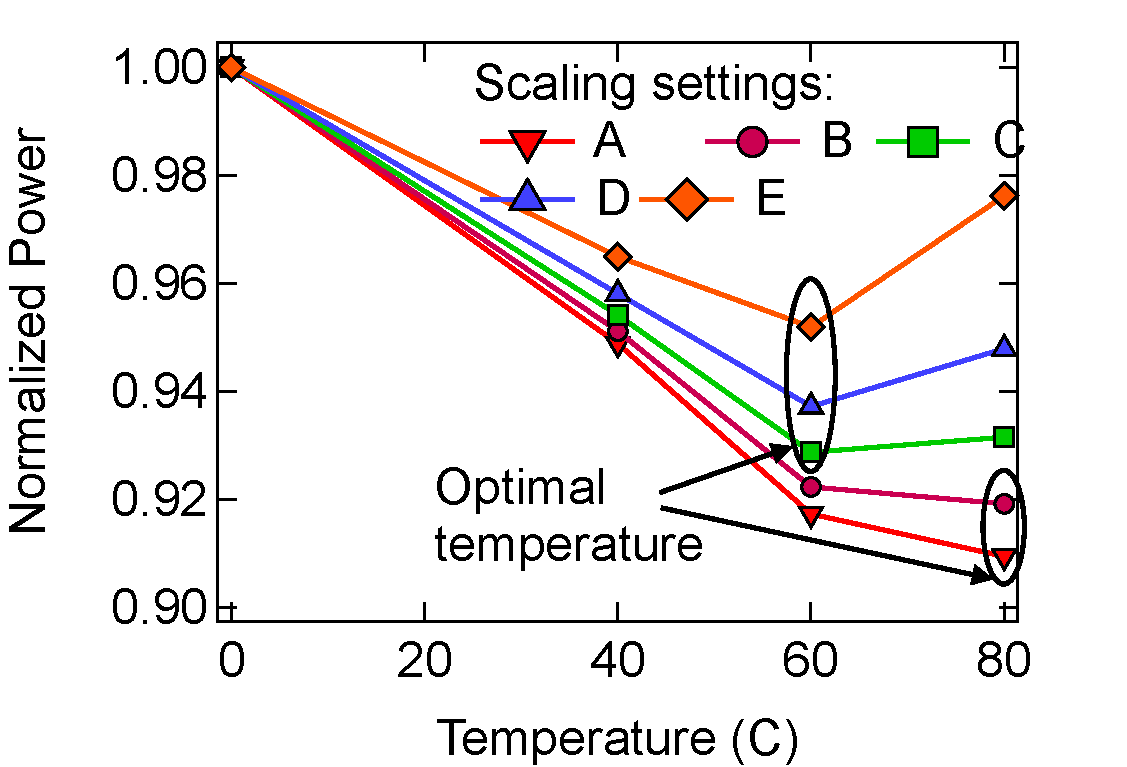
\includegraphics[trim=0 0 40 0,clip,width=0.47\linewidth]{graphs/temperature/FFT-diff-factor.pdf}
    \label{fig:scale-FFT}
  }
  \endgroup
  \hfill
  \begingroup
  \captionsetup[subfigure]{width=0.\linewidth}
  \subfloat[Benchmark \benchmark{particlefilter}] 
  {
    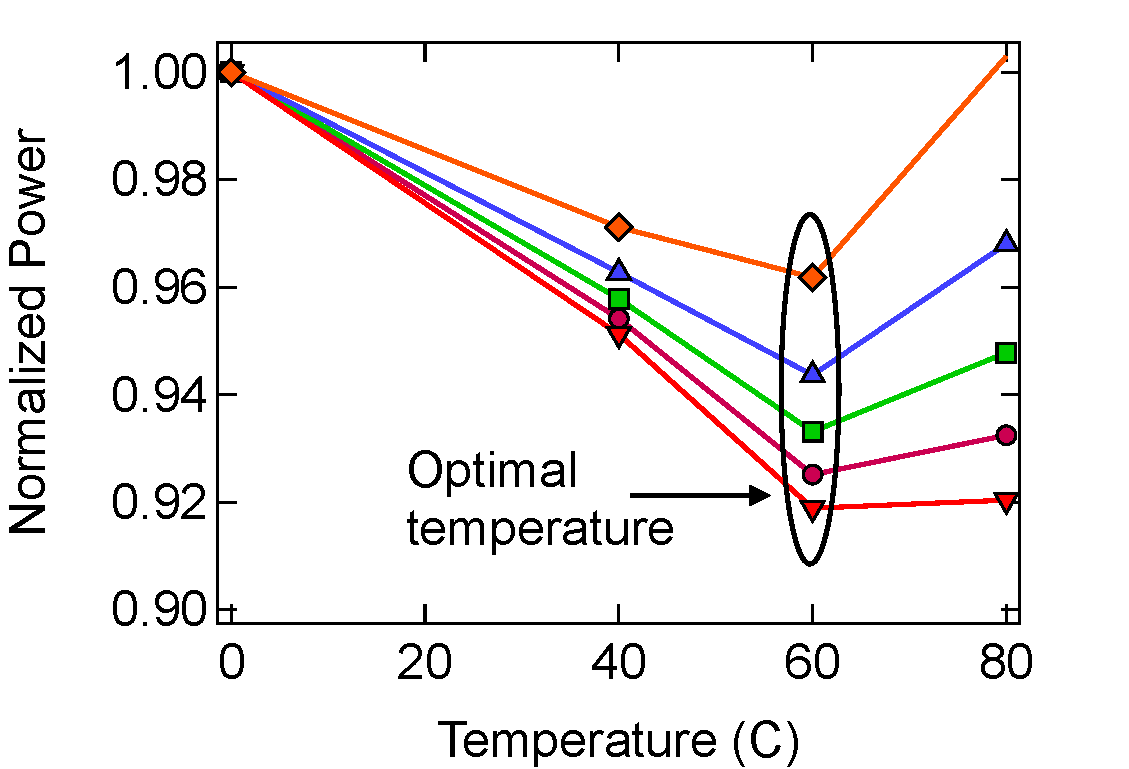
\includegraphics[trim=0 0 40 0,clip,width=0.47\linewidth]{graphs/temperature/particlefilter-diff-factor.pdf}
    \label{fig:scale-particlefilter}
  }
  \endgroup

  \begingroup
  \captionsetup[subfigure]{width=0.3\linewidth}
  \subfloat[Benchmark \benchmark{Reduction}] 
  {
    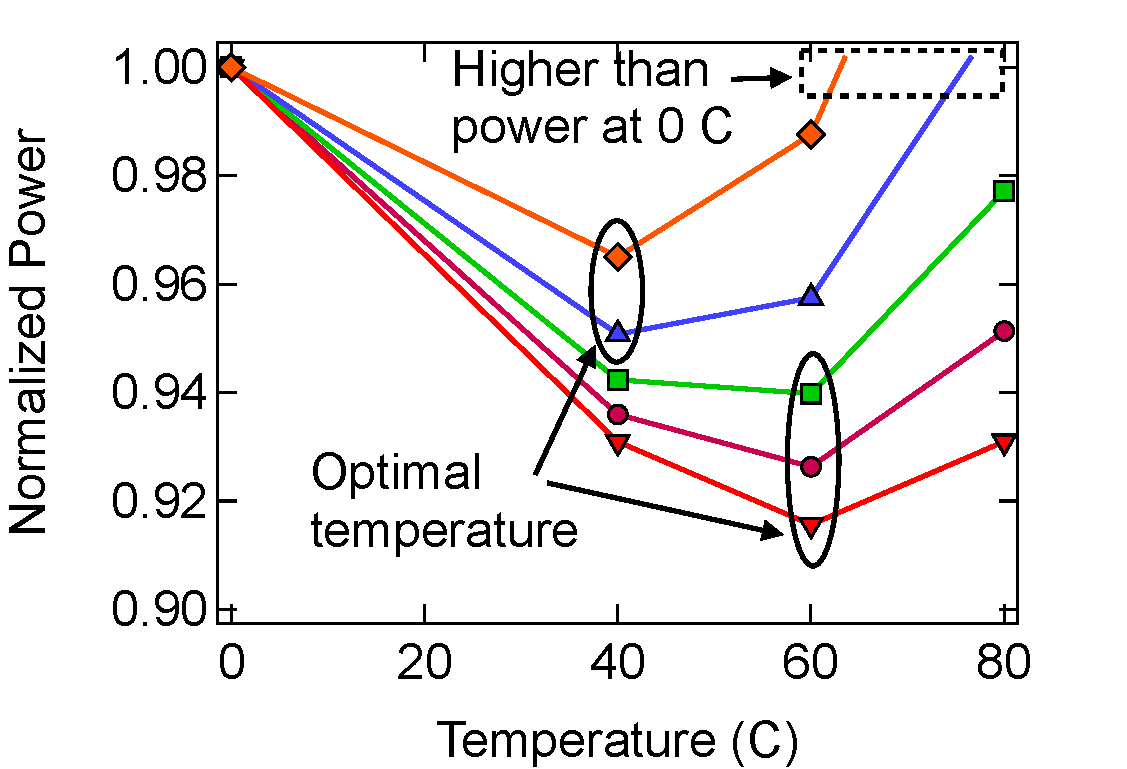
\includegraphics[trim=0 0 40 0,clip,width=0.47\linewidth]{graphs/temperature/Reduction-diff-factor.pdf}
    \label{fig:scale-Reduction}
  }
  \endgroup
  \caption{Power versus temperature at different scaling factors for different workloads. In FinFET and FD-SOI, \tistate makes GPU power smaller at high temperature. The optimal temperature is different for the workloads and the different scaling settings, and this is because the ratio of static to dynamic power across the workloads varies.}
  \label{fig:scale-analysis}
\end{figure}


In FinFET and FD-SOI, the scenario above will fundamentally change. FinFET and FD-SOI have much less leakage power, therefore the leakage power increase has a smaller effect on overall processor power under higher temperature. The opposite side is the more salient dynamic power improvement caused by \tistate's voltage reduction. These two opposite trends form a trade-off: an optimal temperature may exist where \tistate's dynamic power reduction balances leakage power increase at higher temperatures and the overall processor power is minimized. Carefully evaluating this trade-off is crucial for \tistate to be practical in runtime processor temperature and power management control. 

We examine \tistate's power benefits on FinFET and FD-SOI for three different types of workloads that are representative of different typical dynamic-to-leakage power ratios. The workloads include \benchmark{FFT}, \benchmark{particlefilter} and \benchmark{Reduction}, going from high to low dynamic power consumption. \Fig{fig:scale-analysis} shows \tistate's GPU power under different scaling settings. Power is normalized to 0\C to show how power scales as temperature increases. 

\Fig{fig:scale-FFT} shows that when the dynamic power is more dominant in settings \marker{A} and \marker{B} then \benchmark{FFT} prefers to stay at 80\C. Under more conservative settings where leakage power is higher, the temperature sweet spot drops to 60\C. In these scaling settings, FinFET's leakage power increase beyond 60\C is more than \tistate's dynamic power reduction.

For medium dynamic power, \Fig{fig:scale-particlefilter} shows that \benchmark{particlefilter}'s temperature sweet spot is around 60\C for the scaling ratios. \benchmark{Particlefilter}'s dynamic power is not high enough to make \tistate's power saving override leakage power at 80\C. 

In contrast to \benchmark{FFT} and \benchmark{particlefilter}, the workload \benchmark{Reduction} does not consume much dynamic power. \Fig{fig:scale-Reduction} shows that it prefers to stay at a lower temperature to minimize leakage power. Its dynamic power occupies a smaller portion of total power, therefore \tistate's power reduction has a lesser effect. In the optimistic scaling settings \marker{A} and \marker{B}, \benchmark{Reduction}'s sweet spot temperature is 60\C, whereas, in conservative settings \marker{D} and \marker{E}, the optimal temperature is at 40\C to avoid the exponential leakage power at a higher temperature. 

In general, \Fig{fig:scale-analysis} shows that when leakage power is less prominent (i.e., leakage scaling is more aggressive in~\Tab{table:scaling-setting}), \tistates have higher power saving and the optimal temperature is also higher. With smaller leakage, dynamic power occupies a larger portion of the total power, which is when \tistate's improvement has a bigger power saving impact. In the extreme assumption where leakage power is completely agnostic of temperature, \tistate would prefer to operate at the highest allowed temperature to maximize the magnitude of voltage reduction from temperature inversion.

We also find when the optimal temperature is higher, the corresponding optimal power tends to be lower as well.  \tistate's power saving capability increases with higher temperature. When a workload has a larger share of dynamic power and prefers to run under a higher temperature, \tistate's higher power saving manifests as total power improvement.

Another observation that we can make from~\Fig{fig:scale-analysis} is that high-power workloads typically have higher temperature sweet spots. For such workloads, the dynamic power is more dominant than the leakage power. Therefore, in such scenarios, for a given temperature, the percentage of dynamic power saving from \tistate contributes more to the bottom-line.

\subsection{Runtime Temperature Control}
\label{sec:runtime}

\begin{figure*}[t!]
\centering
    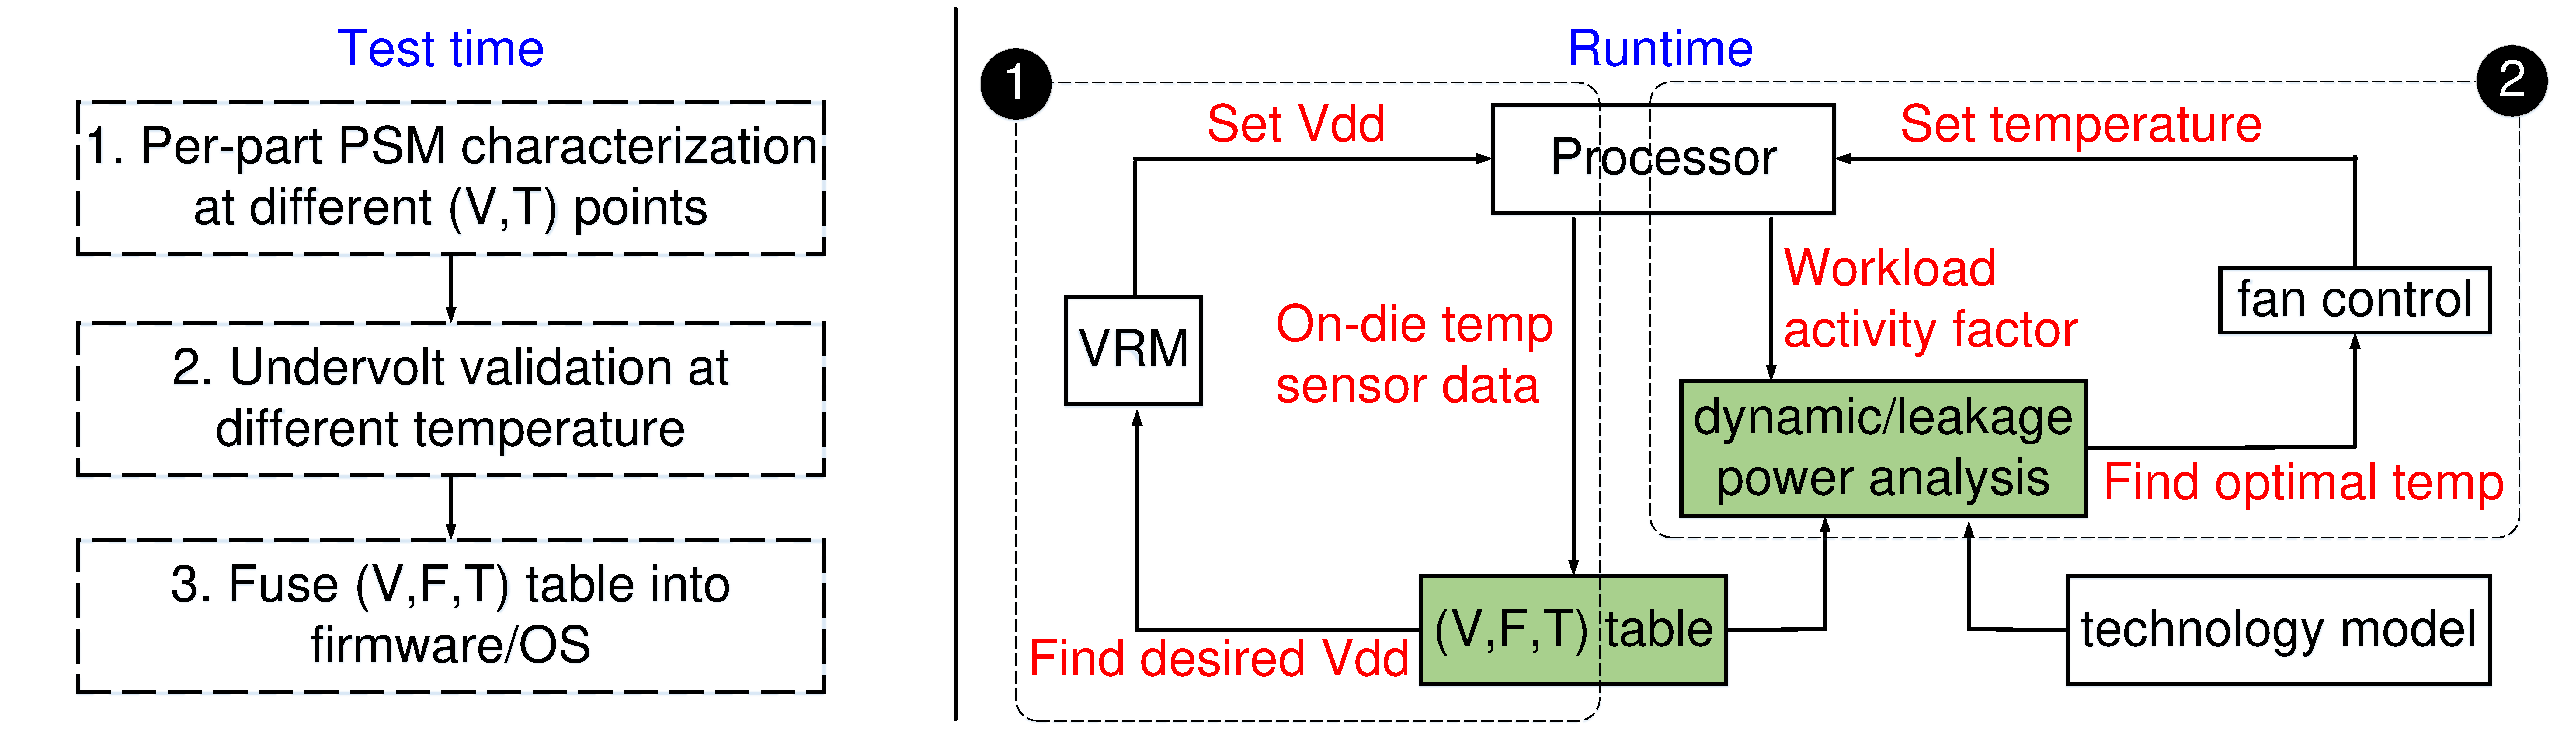
\includegraphics[trim=0 0 0 0,clip,width=.96\linewidth]{graphs/temperature/runtime-mechanism_v3.pdf}
    \caption{\tistate temperature and voltage control: two loops work in synergy to minimize power. Loop~1 is a fast control loop that uses \tistate table to keep adjusting voltage in response to silicon temperature variation. Loop~2 is a slow control loop that sets the optimal temperature based on workload steady-state dynamic power profile.}
    \label{fig:runtime}
    \vspace*{-.1in}
\end{figure*}

We notice that different temperature sweet spots under all workloads and scaling scenarios are essentially a result of processor's dynamic-to-leakage power ratio. To leverage this fact, we propose a set of temperature and voltage control algorithms in~\Fig{fig:runtime} to steer future FinFET and FD-SOI processors for maximum power efficiency. The solution consists of two stages: test-time and runtime.

At test time, the methodology described in~\Algo{train-algo} establishes \tistate's temperature-voltage tables.  The process starts with characterizing the circuit speed behavior with on-chip timing sensors like the PSM, which are subsequently verified by workload timing margin measurements as we described earlier. The final temperature-voltage table can be fused into firmware for runtime lookup. For each chip, we envision less than 40 entries to be added in total. Constructing such tables is already in practice~\cite{sriram2016avfs}. It only extends the existing test flow by a few steps and adds minimal overhead.

At runtime, two loops work in synergy. Loop 1 is a fast loop that addresses quick yet small temperature variations from workload phase changes. It measures silicon temperature and index into \tistate table in real time to get and set the desired voltage, similar to a typical DVFS table lookup. We envision this loop to occur at millisecond-level granularity, as in with other systems~\cite{lefurgy2011active}. Loop 2 is a slow control loop that monitors the workload's average activity factor over a longer time period to estimate its dynamic-to-leakage power ratio. This ratio is used to find the optimal temperature in~\Fig{fig:scale-analysis}, and hence discovers the \tistate's optimal long-term average voltage.

We envision that loop 2 will target the average power savings over a relatively long time (seconds or longer). This is because runtime temperature control by adjusting the cooling system is a relatively slow process. Many of today's workload have steady state behavior suitable for this behavior, such as scientific and deep learning applications, as well as web service workloads that have diurnal patterns~\cite{lo2014towards}. Thus, it is feasible to enable power saving in this scenario.

\section{Related Work}
\label{sec:temperature:related}

Temperature inversion has been reported for CMOS devices long before~\cite{park1995reversal,bellaouar1998supply,dasdan2006handling,wolpert2012temperature}. These works address the reason for this phenomenon, largely at the device level. Recent works study temperature inversion in FinFETs~\cite{lee2014dynamic,cai2015tei}. Our work, however, is the first to systematically measure and characterize temperature inversion under 28 nm process and discuss its implications to the architecture and its power management. 

Adaptive voltage setting for temperature variation has been recently proposed~\cite{sriram2016avfs}. \tistates work in a similar way to the lookup table that the authors propose. However, our work focuses on the temperature's effect in the inversion region and provides an in-depth analysis, while the solution in~\cite{sriram2016avfs} mixes process and temperature variation together. Moreover, prior work does not address the implications of temperature control in future technologies, as we do with our FinFET analysis.

Active timing guardband management using on-chip sensors has been recently proposed~\cite{lefurgy2011active,zu2015adaptive}. These prior works focus mostly on transient $di/dt$ droop and its effect on the timing margin. In contrast, we use PSMs to characterize temperature inversion and its effect on the timing margin. We also study temperature inversion's effect in an integrated manner with $di/dt$ droop and discuss the relationship between the two.

Many papers have addressed architecture-level temperature management~\cite{skadron2004temperature,huang2006hotspot,fan2016computational,raghavan2012computational}. These works try to avoid excess high temperature. But we demonstrate experimentally how temperature inversion can make high temperature a friendly environment for runtime power management.


%!TEX root=../paper.tex

\chapter{Architecture and Scheduling Optimization for Active Timing Margin of Voltage Variation}
\label{sec:voltage}

In addition to temperature variation, voltage variation poses unique challenges to active management of processor timing margin. Timing margin must ensure operating reliability under the worst-case, lowest voltage level delivered to transistors, taking into various effects including high loadline, fast $di/dt$ droops, as well as IR drop across the power delivery network (PDN).

In recent years, many hardware techniques have been proposed to  address the high amount of static margin allocated for voltage variation~\cite{kurd2008next,lefurgy2011active,bowman201222nm,grenat20145,tokunaga20145,bowman20158}. These active timing margin solutions schemes aim at reducing the total margin in an agile way to improve system efficiency while still ensuring processor reliability. In this thesis, we present a detailed, full-system characterization of these active timing margin hardware designed specifically for tolerating voltage variation. 

Using measurements and running real-world workloads, we study the factors that affect these active timing margin processors' behavior. Using a fully built production POWER7+ system, we systematically characterize the benefits and limitations of active timing margin in terms of multicore scaling and workload heterogeneity. In our analysis, we cover both active timing margin's undervolting and overclocking modes to fully characterize the system effects under different usage scenarios. 

We find when only one core is active, the current hardware active timing margin schemes can efficiently turn the underutilized timing margin into significant power and performance benefits while tolerating voltage swings. However, as more cores are progressively utilized by a multithreaded application, the benefits of active margin begin to diminish in both power and performance improvements. Using POWER7+'s sensor-rich features, we systematically characterize and decompose the on-chip voltage drop that affects the active timing margin's efficiency into its different components, and analyze the root cause of the problem. Under heavy load, the IR drop across the chip and the voltage regulator module's (VRM) loadline effect limit active timing margin's ability to the point of almost no benefit. 

The magnitude of the efficiency drop aforementioned, however, varies significantly from one workload to another. Thus, given the workload sensitivity of hardware active timing margin techniques, and the long-term nature of the observed effects, we introduce the notion of \emph{adaptive margin scheduling (AMS)}. The intent behind AMS is to compensate for active margin's inefficiencies in system software. The remainder of this section is structured as follows: \Sec{sec:voltage:background} provides background for the POWER7+ architecture and its implementation of active timing margin for voltage variation. \Sec{sec:voltage:characterization} characterizes active margin's limitations when scaling up the number of active cores under different workload scenarios. \Sec{sec:voltage:rootcause} analyzes the root cause of active margin's behavior as seen in the previous section. \Sec{sec:voltage:opt} proposes active timing margining scheduling to improve POWER7+'s efficiency when the load is light versus heavy. \Sec{sec:voltage:related} compares our work with prior work.

\section{Active Timing Margin in the POWER7+ Multicore Processor}
\label{sec:voltage:background}

\TODO{to be merged with the next chapter}

The POWER7+ is an eight-core out-of-order processor manufactured on a 32-nm process. It supports 4-way simultaneous multithreading, allowing a total of 32 threads to execute simultaneously on the system~\cite{manousopoulos2012characterizing}.

A POWER7+ processor has two main power domains, each with its own on-chip power delivery network (PDN). The V$_{dd}$ domain is dedicated to the logic circuits in the core and caches, and the V$_{cs}$ domain is dedicated for the on-chip storage structures~\cite{zyuban2013ibm,barth201045nm}. The PDNs are shared among all eight cores to reduce voltage noise~\cite{james2007comparison}. In our study, we primarily focus on voltage variation over the logic circuits's power domain as it is the main power consumer.

The processor supports both coarse-grained and fine-grained power management. Coarse-grained power management includes per-core power gating to reduce idle power consumption. Fine-grained power management is the active timing margin. In our later AMS optimization, we combine these two schemes to enhance the processor's overall efficiency.

POWER7+ uses active timing to prevent circuit timing emergencies~\cite{lefurgy2011active,lefurgy2013active,floyd2013runtime}. Although the implementation of active timing margin for voltage variation can vary from one platform to another~\cite{fischer200590nm,tschanz2007adaptive,kurd2008next,lefurgy2011active,bowman201222nm,grenat20145,tokunaga20145,bowman20158}, the general building blocks and principles largely remain the same. 
In POWER7+, clock cycle time is variable and actively tracks circuit speed from cycle to cycle. In the event of a voltage droop, the processor slows down the cycle time to allow circuit operation to complete. Because voltage droops occur rarely, during normal operation the active timing margin mechanism eliminates a significant portion of the timing slack.

\begin{figure*}[t]
\centering
\subfloat[Control loop overview.] {
   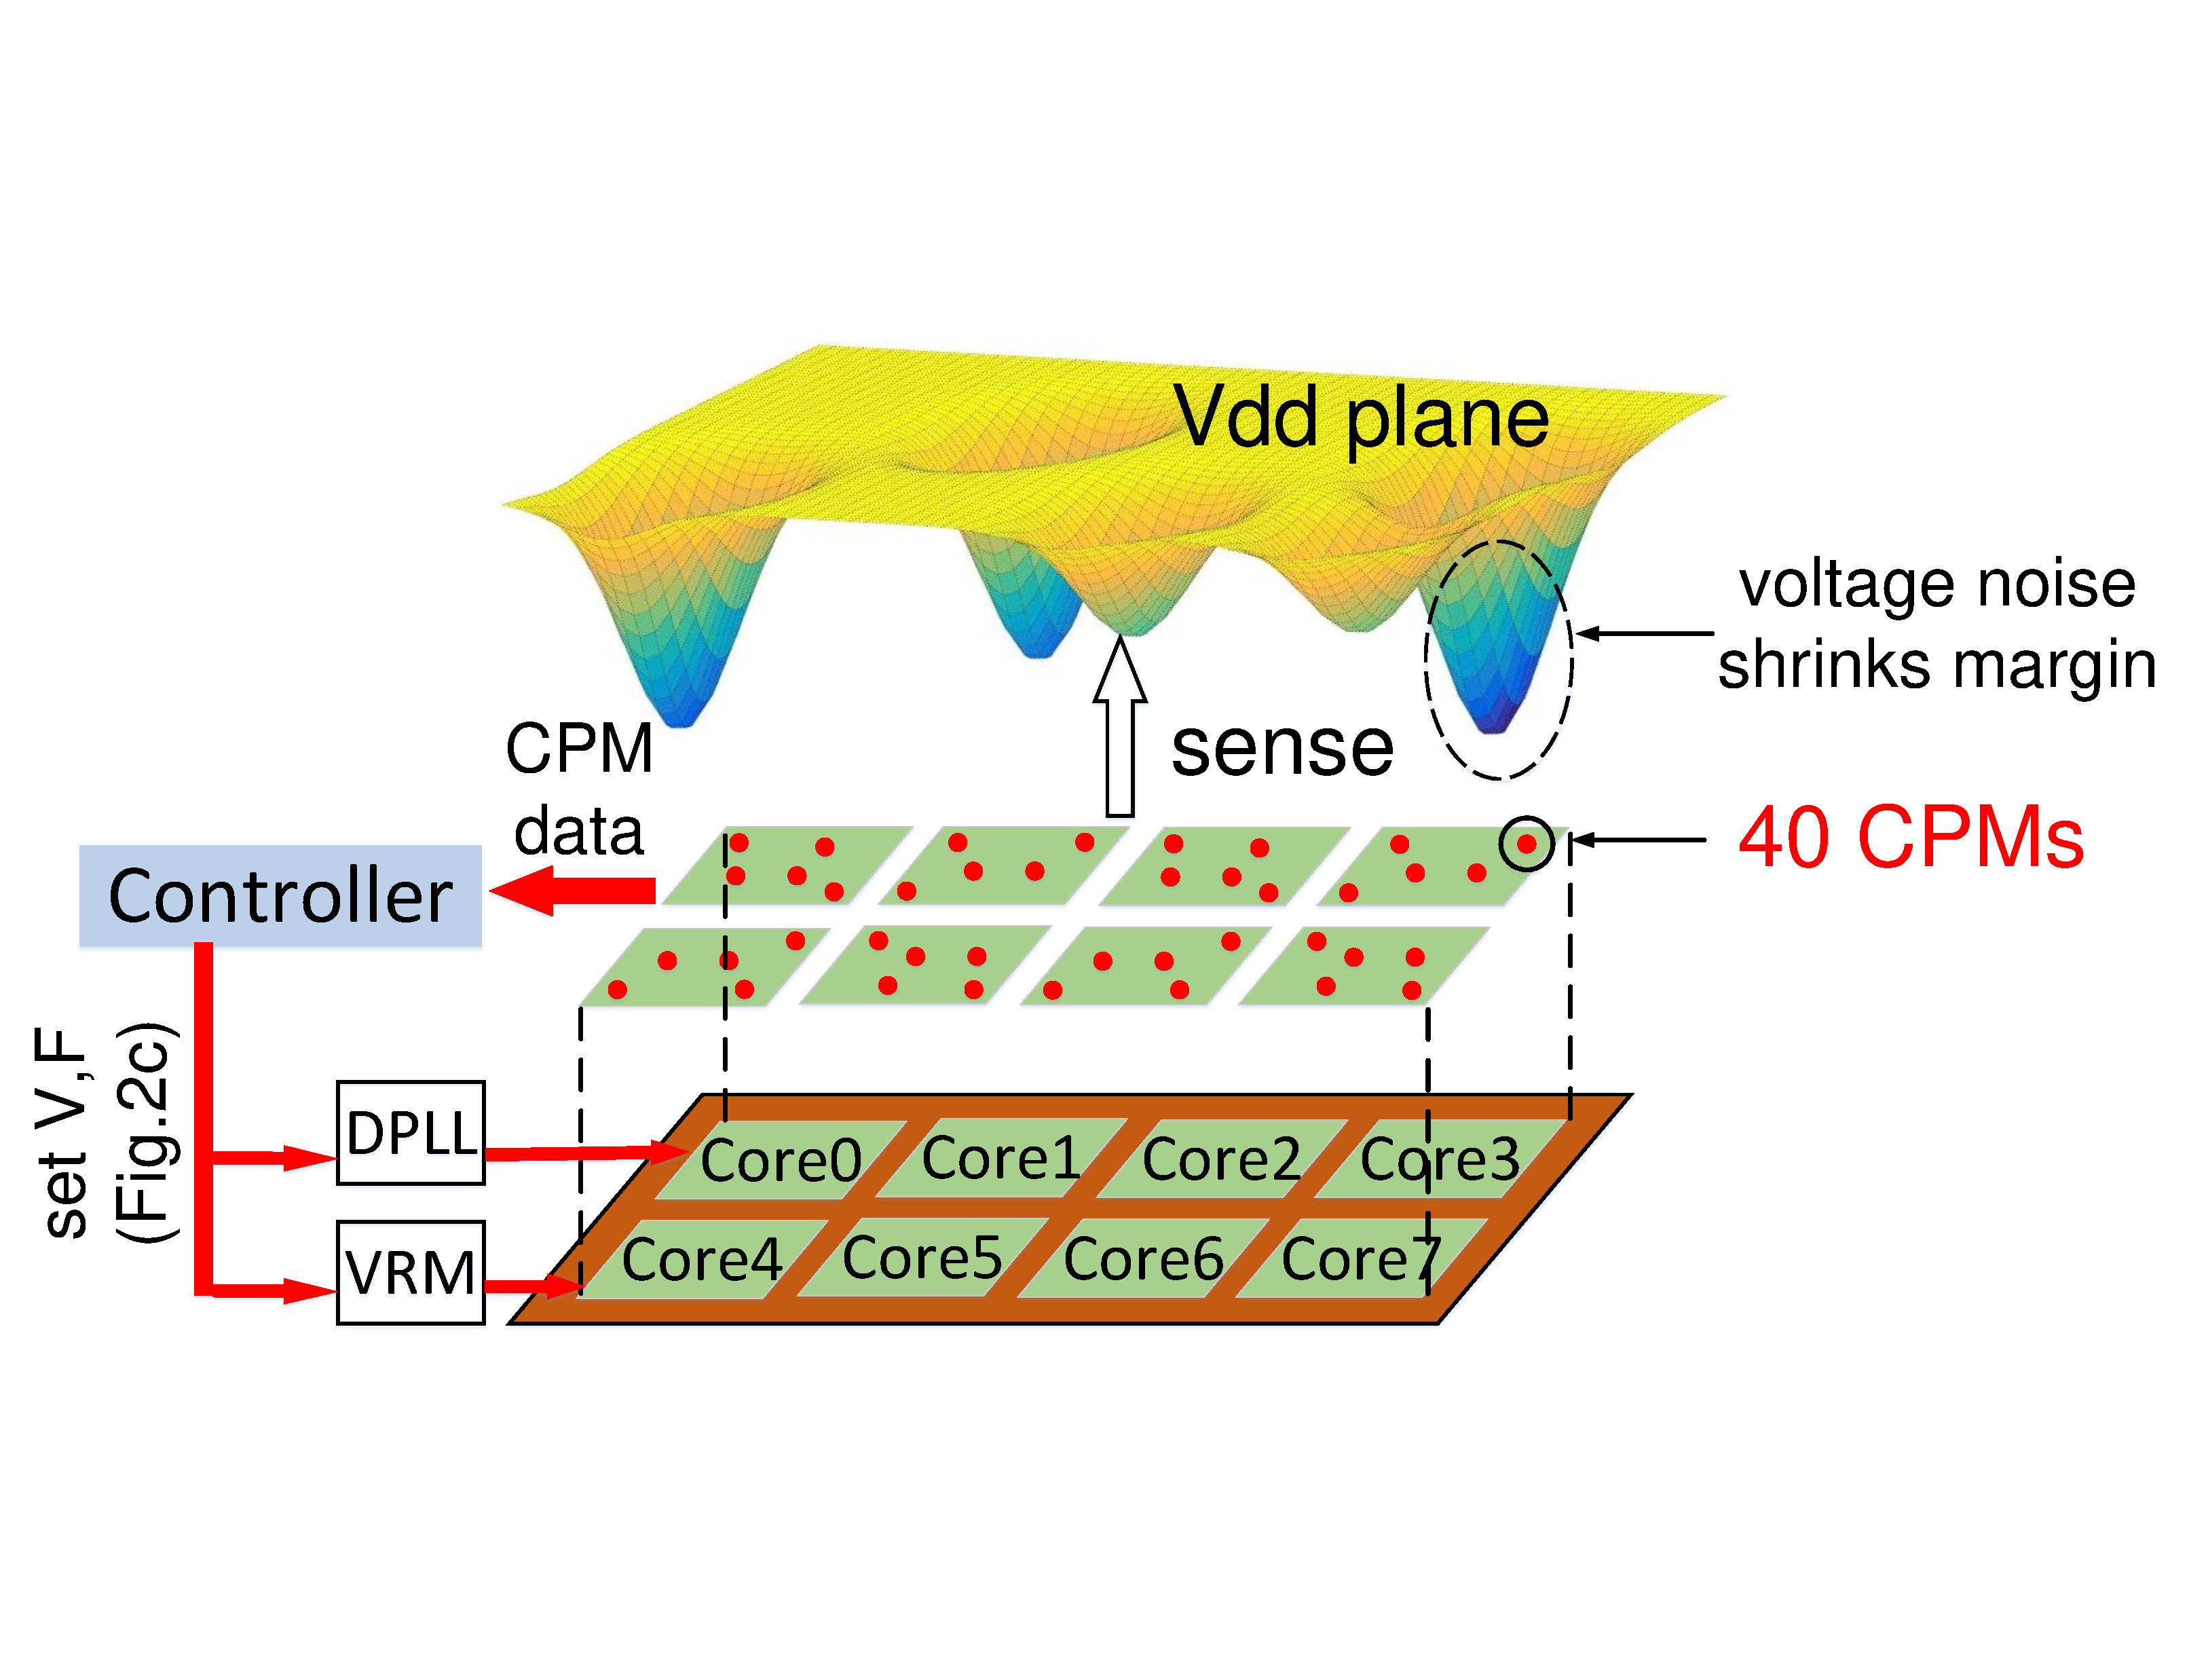
\includegraphics[trim=0 250 0 260,clip,width=.625\linewidth]{graphs/voltage/control-loop.pdf}
   \label{fig:control-loop} 
}
\subfloat[CPM behavior.] {
   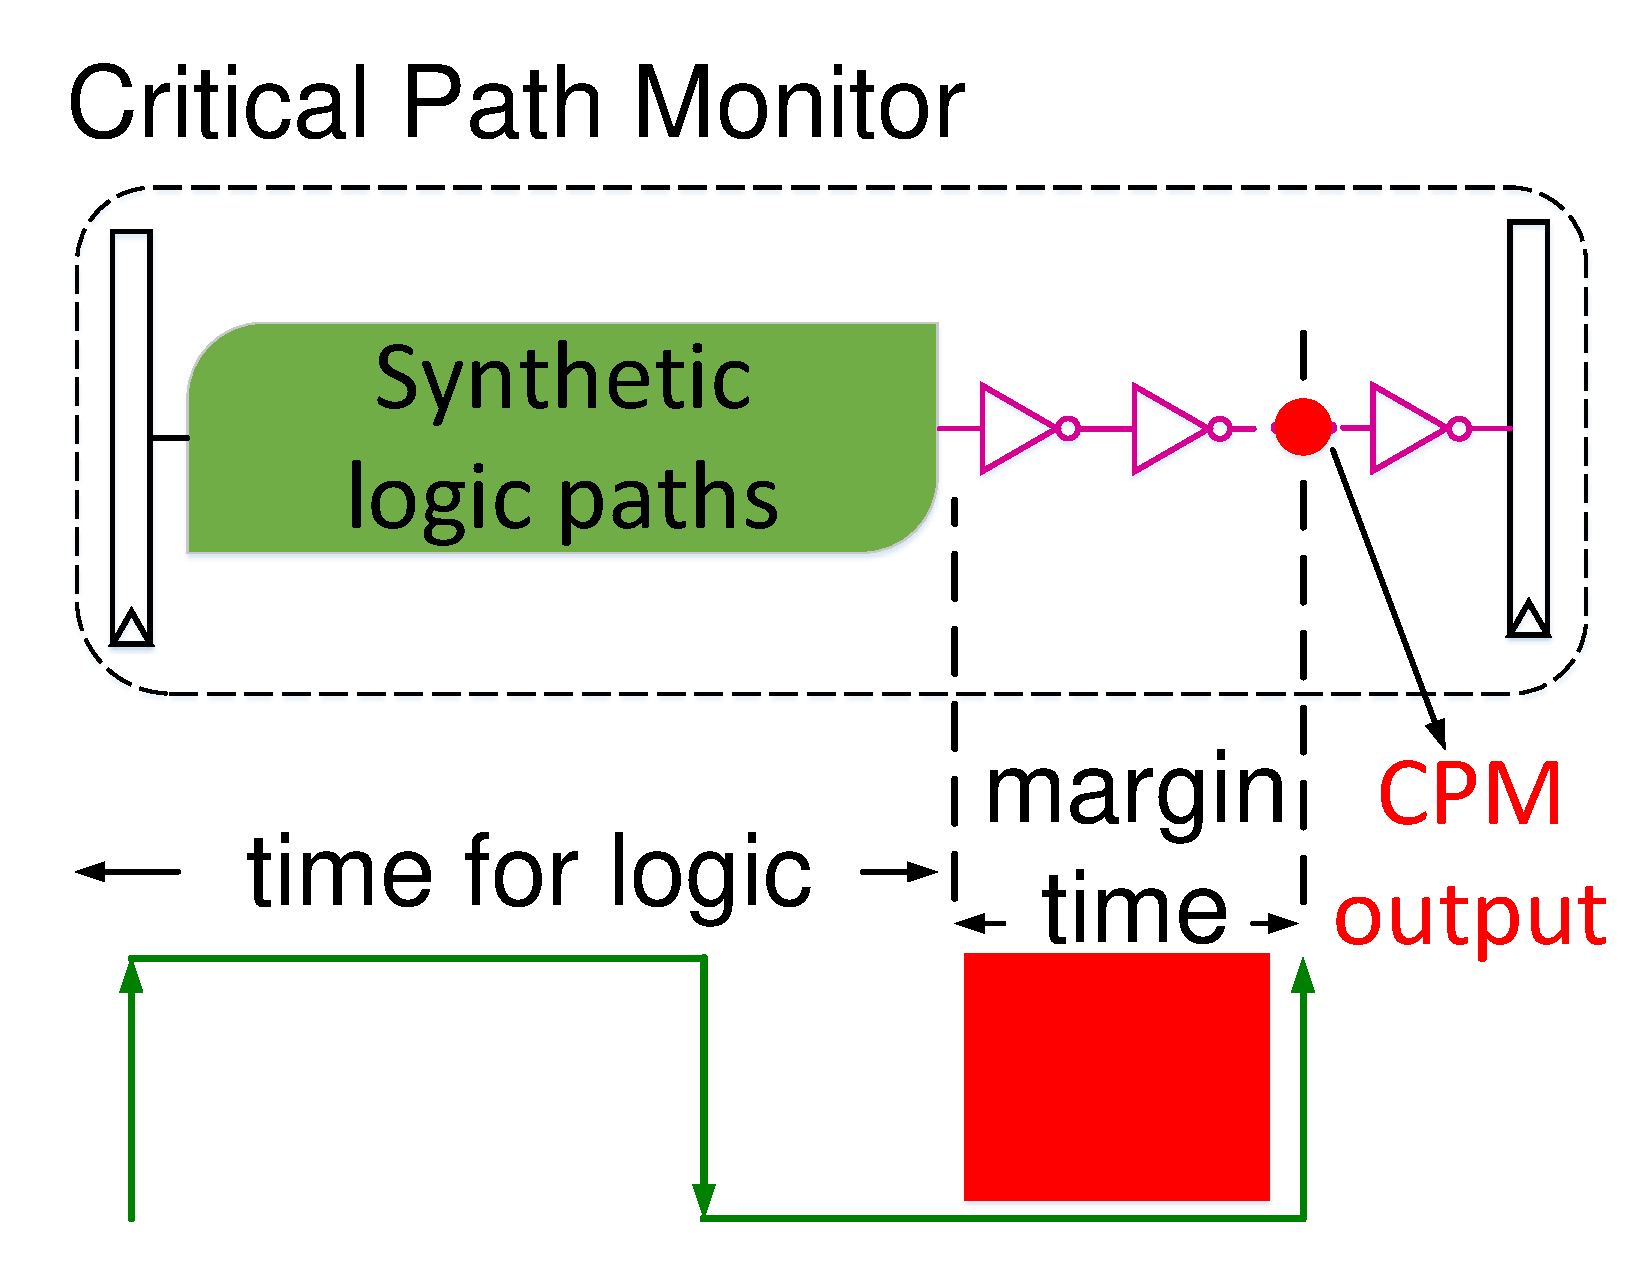
\includegraphics[trim=0 20 0 20,clip,width=.385\linewidth]{graphs/voltage/CPM-structure.pdf}
   \label{fig:cpm_internal} 
}
\caption{Interactions among CPMs, DPLLs, and VRMs to guarantee reliability and improve efficiency in POWER7+. CPM measures the timing margin and the controller adjusts voltage and frequency accordingly.}
\end{figure*}

\Fig{fig:control-loop} shows an overview of the feedback loop for active timing margin control. The system relies on three key components: (1) critical path monitor (CPM) sensors to sense timing margin~\cite{drake2007distributed,drake2013single}; (2) digital phase locked loops (DPLLs) to quickly and independently adjust clock frequency per core based on CPM readings~\cite{tierno2010dpll}; and (3) hardware and firmware controllers that decide when and how to leverage the benefits from a tighter timing margin.

POWER7+ has 40 CPMs distributed across the chip to provide chip-wide, cycle-by-cycle timing margin measurement. Each core has 5 CPMs placed in different units to account for core-level spatial variations in voltage noise and critical path sensitivity. Detailed characterization of CPM placement, calibration, and sensitivity is provided in~\cite{floyd2013runtime}.

A CPM uses synthetic paths to mimic different logical circuits' behavior and a 12-bit edge detector to quantify the amount of timing margin left. \Fig{fig:cpm_internal} illustrates the CPM's internal structure. On each cycle, a signal is launched through the synthetic paths and into the edge detector. When the next cycle arrives, the number of delay elements the edge has propagated through in the edge detector corresponds to the CPM output. A CPM outputs an integer index from 0--11, which corresponds to the position of the edge in the edge detector.

In the POWER7+ processor, during chip testing the different CPMs are calibrated to output a target value.  When the output is less (toward zero), the timing margin has been reduced from the calibrated point. Likewise, when the output is more (toward 11), the available timing margin has increased.

Per-core DPLL frequency control lets the processor tolerate transient voltage droops by reducing clock frequency for each core with no impact on other cores. The DPLLs can rapidly adjust frequency, as fast as 7\% in less than 10 ns, while the clock is still active; thus, the processor can tolerate transient voltage droops. Every cycle, the lowest-value CPM in each core is compared against the calibration position. In response, the DPLL will slew the clock frequency up or down to control the timing margin to the calibrated amount. 

POWER7+ supports two modes to convert the excess timing margin into either a performance increase by overclocking or power reduction by undervolting. In the overclocking mode, the CPM and DPLL hardware form a closed-loop controller. At the fixed nominal voltage, the DPLL continuously adjusts frequency on the basis of the CPM's timing sense to operate at the calibrated timing margin. Under light loads, clock frequency can be boosted by as much as 10\% compared to when active timing margining is off. In the undervolting mode, the firmware observes CPM-DPLL's frequency and over a longer term (32ms) adjusts voltage to make clock frequency hits the target. In this case, the performance benefit from the CPM-DPLL can be turned into an energy-saving benefit.

\section{Efficiency Analysis of Active Timing Margin on Multicore}
\label{sec:voltage:characterization}

Most prior art studied the benefits of mitigating voltage variation and reducing timing margin at the circuit-~\cite{kurd2008next,bowman201222nm,grenat20145,tokunaga20145,bowman20158} and architecture levels~\cite{lefurgy2011active,reddi2009voltage,gupta2008decor,powell2003pipeline,reddi2010voltage,bertran2014voltage} using homogeneous single-core workloads. This thesis focuses on understanding the efficiency of active timing margin on a multicore system, specifically as the system activity (i.e., core usage) begins to increase using real workloads.

Using an enterprise class server (\Sec{sec:voltage:characterization:setup}), we characterize the efficiency of active timing margin at the system level. In particular, we measure, analyze and characterize active timing margin's effectiveness under different architectural configurations and workload characteristics. We make two fundamentally new observations about the effectiveness of active timing margin on a multicore system. First, the efficiency of active timing margin can diminish as the number of active cores increases (\Sec{sec:voltage:characterization:scaling-trends}). Second, the inefficiency is highly subject to workload characteristics (\Sec{sec:voltage:characterization:workload-variation}).

\subsection{Experimental Infrastructure}
\label{sec:voltage:characterization:setup}
 
We perform our analysis on a commercial IBM Power 720 Express server (7R2) that has two POWER7+ processors on the motherboard. The processors share the main memory and other peripheral resources, such as storage and network. We focus on one of the two processors, although we validated our conclusions by conducting experiments on the other processor as well. Unless stated otherwise, the first processor is configured to idle and runs background tasks. The system runs RedHat Enterprise Linux, configured with 32~GB RAM. 

We use PARSEC~\cite{bienia2008parsec} and SPLASH-2~\cite{woo1995splash,bienia2008parsecsplash} in this section because they are scalable workloads and we need to the control the applications' parallelism to carefully study the impact of core scaling. The workloads are compiled using GCC with \texttt{-O2} optimization.

We characterize the efficiency of active timing margin across two modes of operation: 1) undervolting to reduce power consumption and 2) overclocking to boost performance. Hooks in the firmware let us place the system in either operating mode. The hardware and firmware autonomously select frequency and voltage depending on the configured operation mode.

\subsection{Core Scaling}
\label{sec:voltage:characterization:scaling-trends}
Using \benchmark{raytrace} from PARSEC (as an example), we show active timing margin's impact on chip power. We study both average chip power consumption and total CPU energy savings using \Fig{fig:raytrace-inefficiency}. We find that active timing margin is always effective at improving performance or lowering power consumption. However, it cannot always scale up efficiently with more cores. 

\begin{figure}[t]
	\centering
    \subfloat[Power saving.] {
      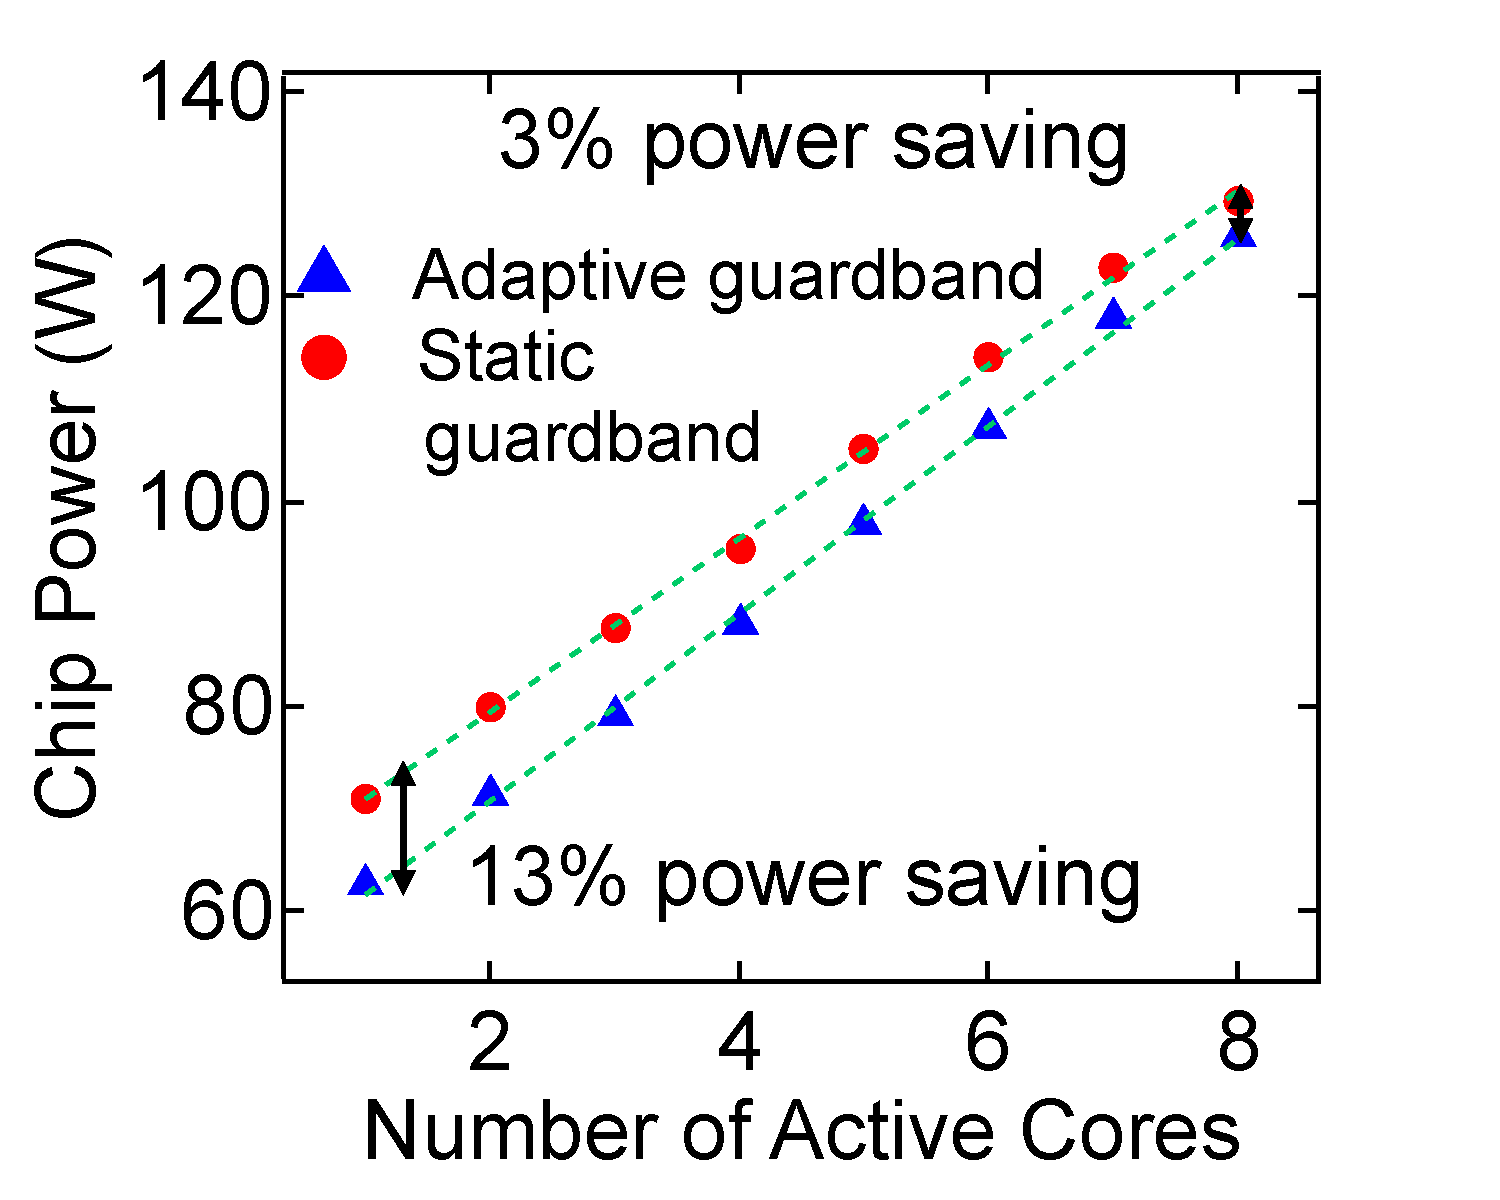
\includegraphics[trim=0 0 0 0,clip,width=.4\linewidth]{graphs/voltage/raytrace_pwr.pdf}
      \label{fig:raytrace-ineff_pwr} 
    }
    \subfloat[Energy reduction.] {
       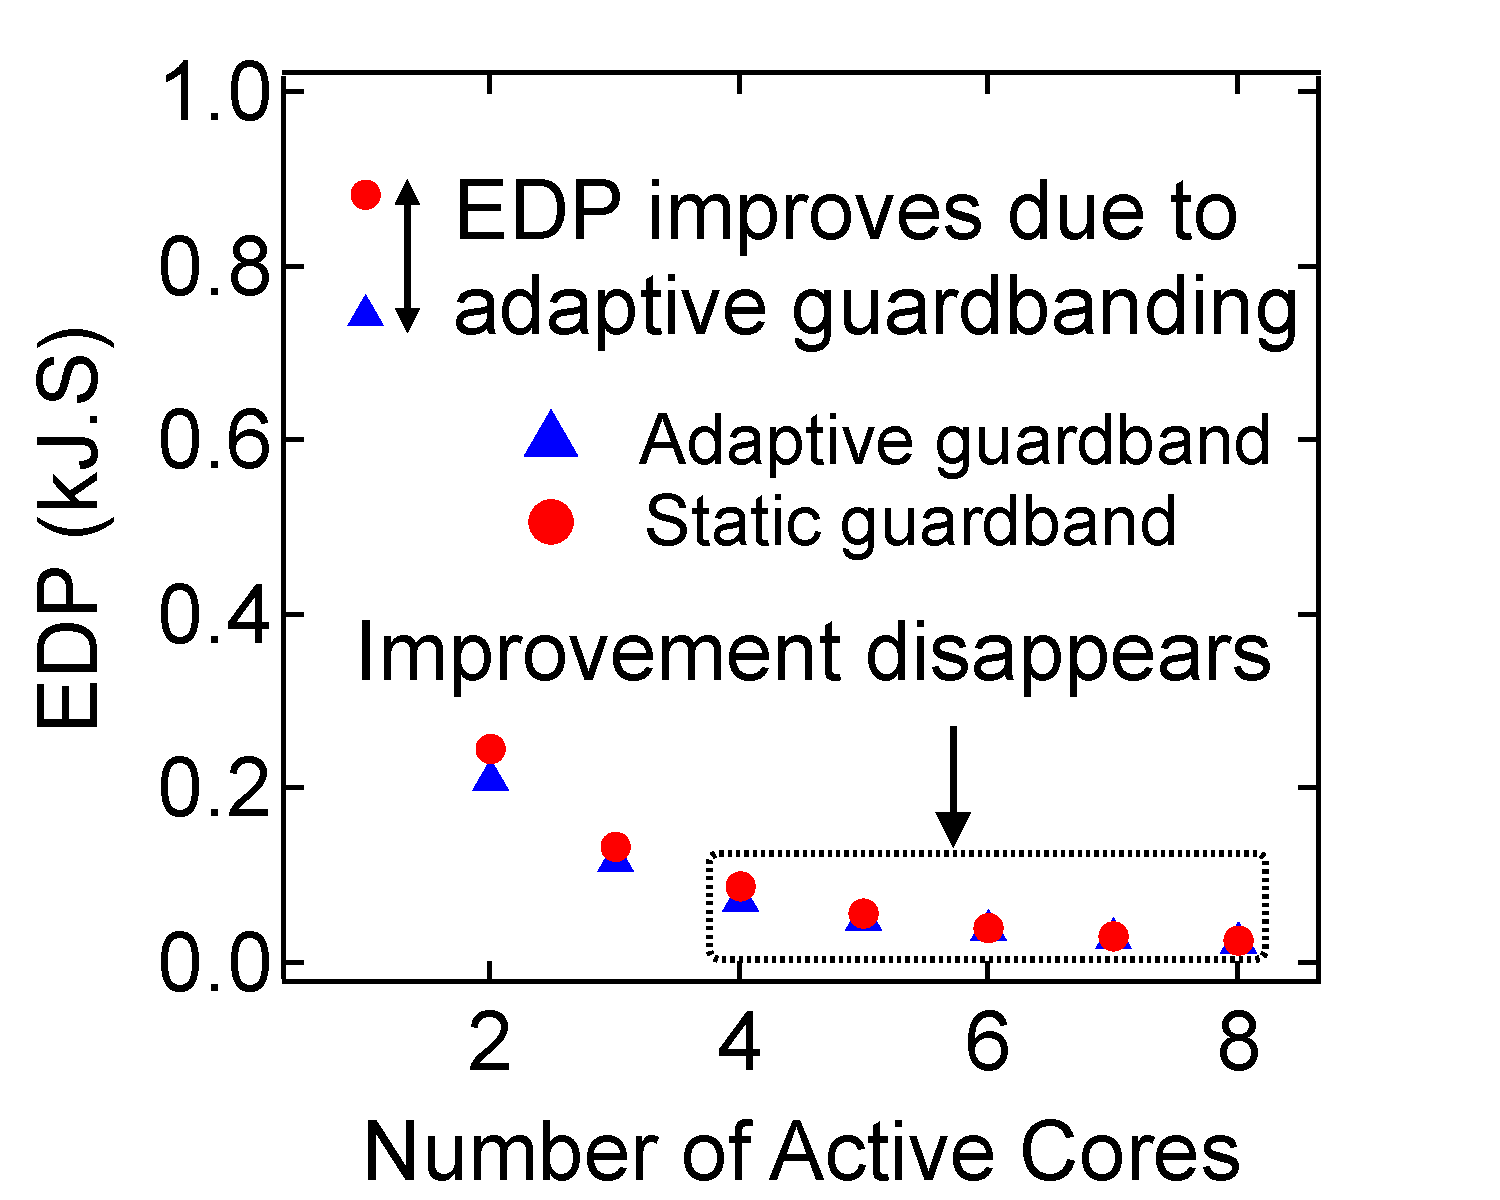
\includegraphics[trim=0 0 0 0,clip,width=.4\linewidth]{graphs/voltage/raytrace_edp.pdf}
       \label{fig:raytrace-ineff_edp} 
    }
    \caption{Active timing margin can save power effectively. However, the benefits decrease as more cores are used to actively run the application.}
    \label{fig:raytrace-inefficiency}
\end{figure}

\Fig{fig:raytrace-ineff_pwr} shows the program's power consumption as we use more cores, i.e., more threads to process the workload. We measure the microprocessor V$_{dd}$ rail power by reading physical sensors available on the server, which represents most of the total processor power. In undervolting mode, active timing margin turns the unused margin into energy savings by scaling back the voltage, which reduces unnecessary power consumption. When one core is active and the others are idle, active timing margin reduces the average power consumption by 13\% compared to no active timing margining. 

Although active timing margin always saves power, a more important and crucial observation from \Fig{fig:raytrace-ineff_pwr} is the decreasing power-saving trend as the number of active cores increases in the system. The power improvement from active timing margin decreases as the parallelism in the workload is (manually) increased, forcing the usage of the additional cores. Although active timing margin can save as much as 13\% power when only one core is active, the savings drop sharply to about 3\% when the activity scales up to eight cores.

When examining the workload's overall energy-delay product (EDP), \Fig{fig:raytrace-ineff_edp} shows notable energy efficiency improvement when only a small set of cores is actively processing the workload. However, beyond four cores, the improvement drops significantly. When only one core is active, processor energy efficiency improves by as much as 20\% compared to using a static margin. But the additional improvement beyond activating more than four cores becomes negligible. 

Our observations hold true for frequency-boosting as well. Active timing margin's ability to boost frequency decreases as core counts increase. \Fig{fig:lucb-inefficiency} shows experimental results for \benchmark{lu\_cb} from the SPLASH-2 benchmark suite. Compared to using a fixed target frequency of 4.2GHz under a static margin, active timing margin can achieve substantial frequency improvement, as shown in~\Fig{fig:lucb-ineff_freq}. When only one core is actively processing the workload, frequency increases by up to 10\% compared to the static margin baseline. However, when all eight cores are running the workload the frequency gain drops to only 4\%.

\begin{figure}
%\vspace*{-.15in}
\centering
    \subfloat[Frequency-boosting mode.] {
        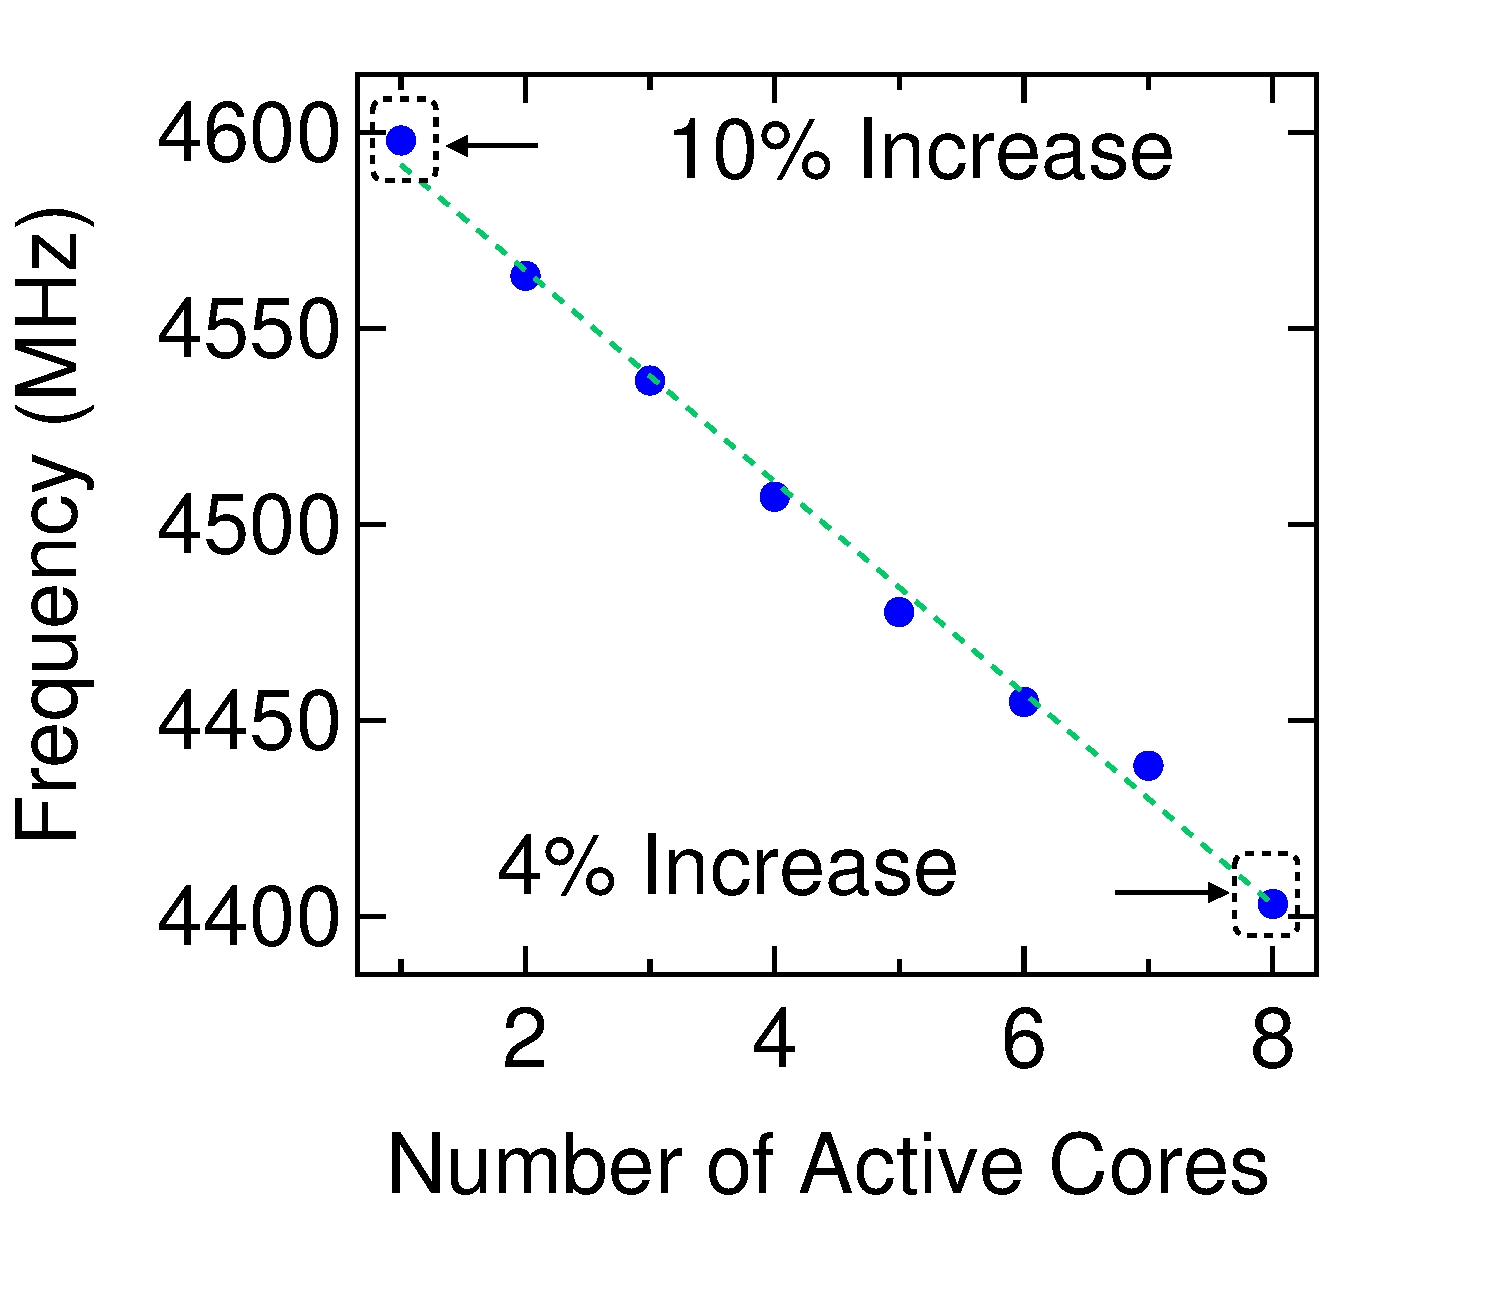
\includegraphics[trim=0 45 65 35,clip,width=.38\linewidth]{graphs/voltage/lucb_freq.pdf}
        \label{fig:lucb-ineff_freq} 
      }
    \subfloat[Execution time.] {
        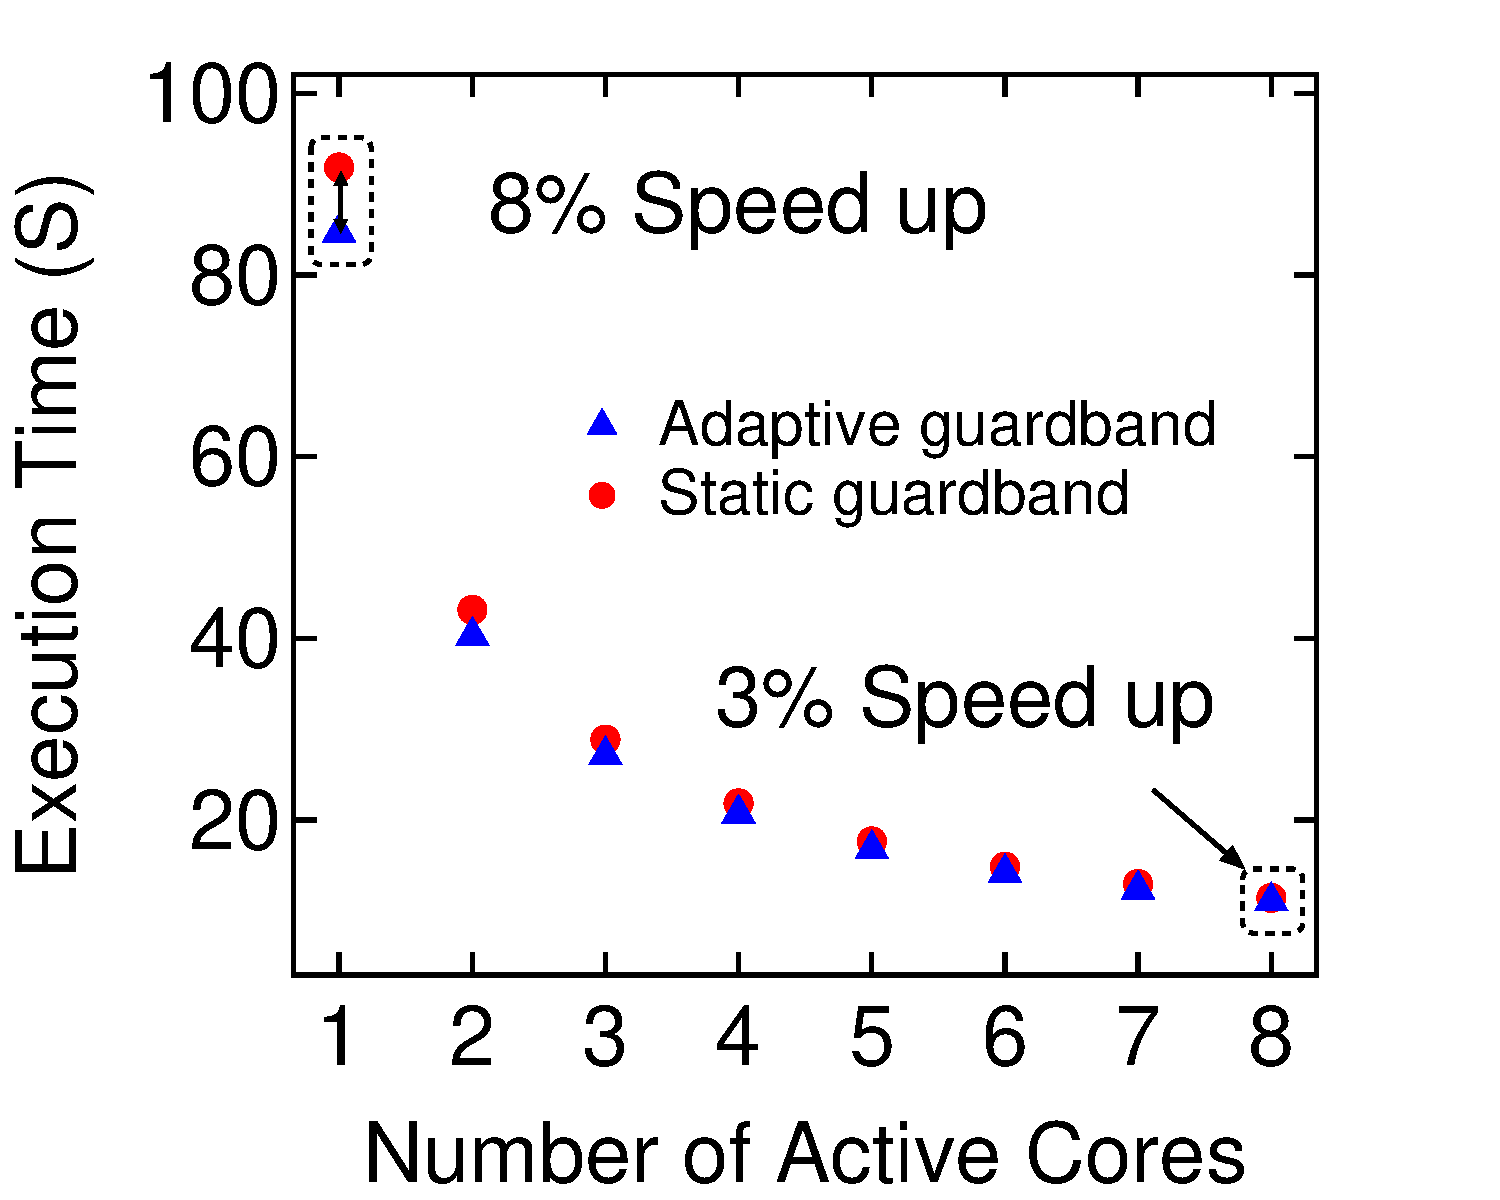
\includegraphics[trim=0 0 65 0,clip,width=.38\linewidth]{graphs/voltage/lucb_time.pdf}
        \label{fig:lucb-ineff_speedup} 
      }
    \caption{Active timing margin can improve performance by increasing frequency. However, the overclocking benefits decrease as more cores are used.}
    \label{fig:lucb-inefficiency}
 \end{figure}

Frequency improvement turns into program execution time speedup, especially for computing-bound workloads. For \benchmark{lu\_cb} the execution speedup varies gradually, decreasing from 8\% when only one core is used to 3\% when all cores are running the workload. This trend of diminishing benefit as core count scales up is similar to what we observe when the extra guardband is turned into energy savings for this workload. 

\subsection{Workload Heterogeneity}
\label{sec:voltage:characterization:workload-variation}

Variations in workload activity (i.e., heterogeneity) are known to strongly impact system performance from cache performance to bandwidth utilization. In this section, we demonstrate workload heterogeneity also impacts active timing margining's runtime efficiency. We focus our analysis on the architecture-level observations and later in \Sec{sec:voltage:rootcause} we explore the causes for the observed behaviors.

\Fig{fig:workloadvariation} shows the results for power and frequency improvement for all PARSEC and SPLASH-2 workloads compared to the same number of cores active when active timing margin is disabled. The improvements are with respect to the system using a static guardband. The results are from two experiments, one in which the control loop is operating in energy-saving mode (\Fig{fig:pwrvariation}) and the other in which it is operating in frequency-boosting mode (\Fig{fig:freqvariation}). Each line in both figures corresponds to one benchmark.

From \Fig{fig:pwrvariation} and \Fig{fig:freqvariation}, we draw four conclusions. First, active timing margining consistently yields improvement, regardless of its operating mode and workload diversity. Across all of the workloads, active timing margining reduces power consumption somewhere between 10.7\% and 14.8\% and improves processor clock frequency by as much 9.6\% on average, when one core is active. Even when all eight cores are active, improvements are at least above 4\%. Power-saving improvements are slightly larger than frequency improvements because of the quadratic relationship between voltage scaling and power, as opposed to the linear relationship between frequency and power.

\begin{figure}[t]
\vspace*{-.15in}
\centering
  \subfloat[Power-saving mode.] {
    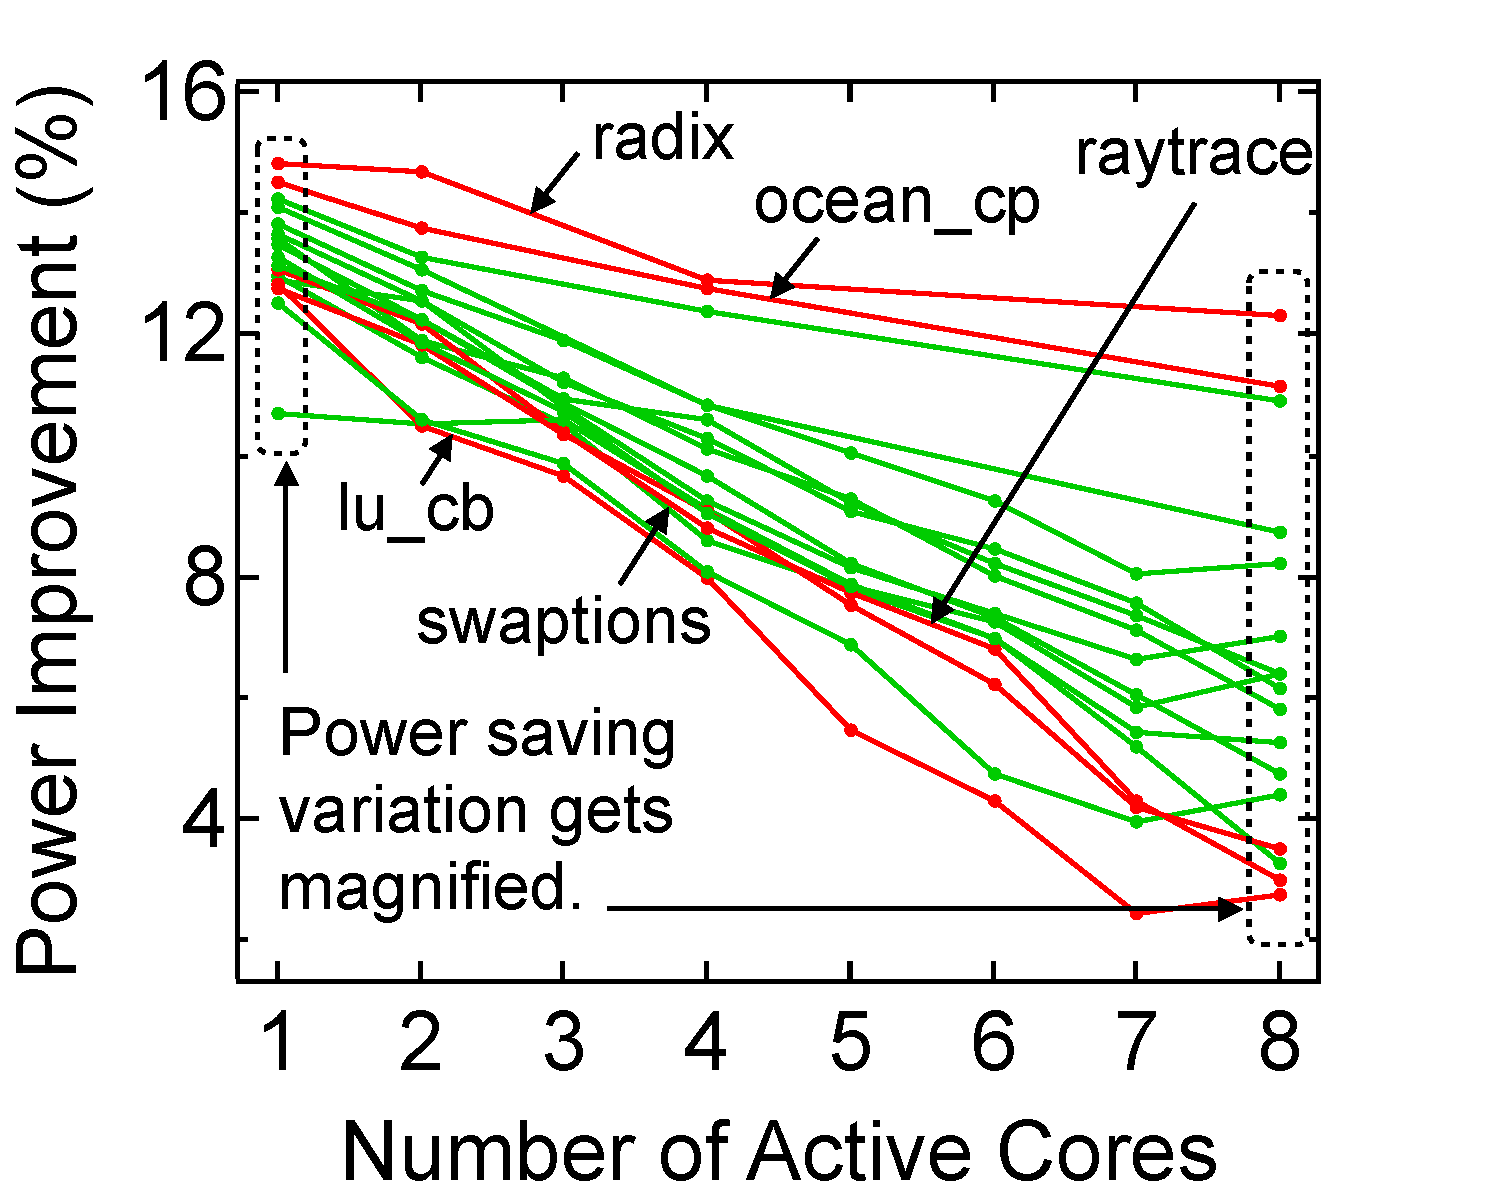
\includegraphics[trim=0 0 0 0,clip,width=.45\linewidth]{graphs/voltage/power_saving_variation.pdf}
    \label{fig:pwrvariation} 
  }
  \subfloat[Frequency-boosting mode.] {
    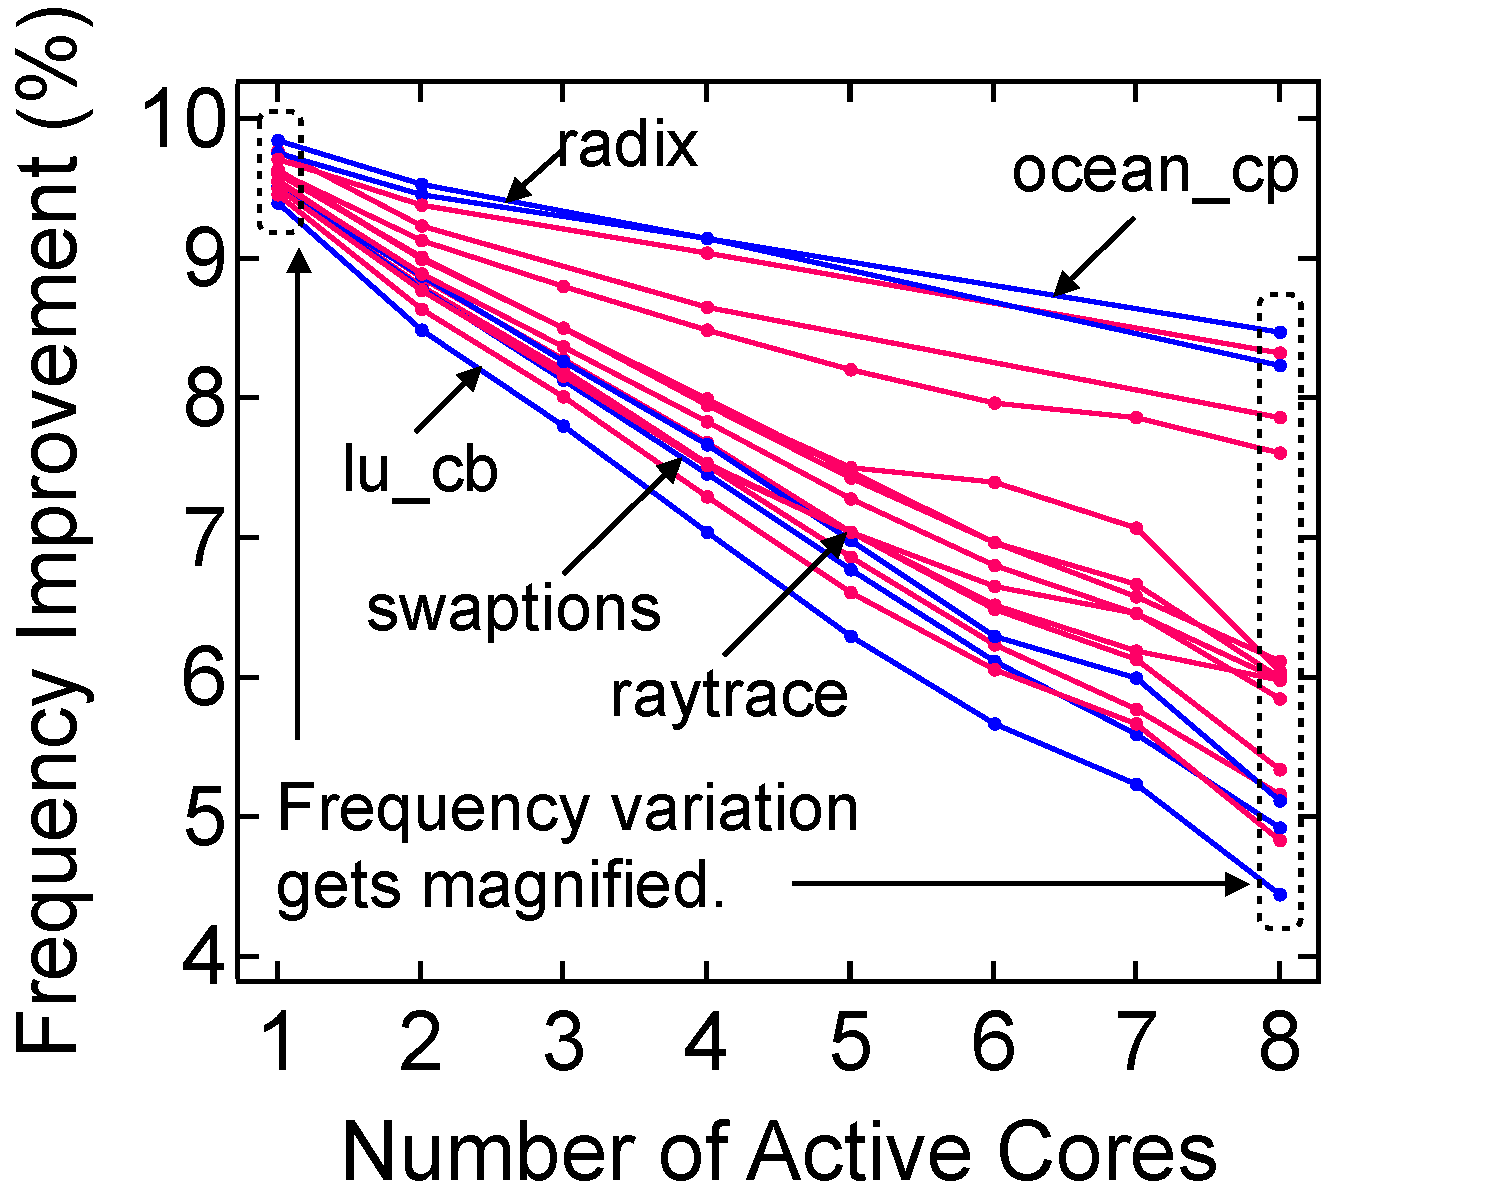
\includegraphics[trim=0 0 0 0,clip,width=.45\linewidth]{graphs/voltage/freq_saving_variation.pdf}
    \label{fig:freqvariation} 
  }
  \caption{Improvements reduce at different rates for each of the PARSEC and SPLASH-2 workloads when cores are progressively activated, leading to magnified workload variation when all cores are active.}
\label{fig:workloadvariation} 
\vspace{-0.2cm}
\end{figure}

Second, the improvements monotonically decrease as the number of active cores increases. Across all the workloads, we observe a consistent drop in active timing margining's efficiency. The average power efficiency improvement across the workloads drops from 13.3\% when one core is active to 10\% when two cores are active to 6.4\% when all cores are actively processing the workload. We observe a similar trend with frequency.

Third, the rate of monotonic decrease for each workload varies significantly. For instance, \benchmark{radix}'s power improvement drops from 15\% when one core is active to around 12\% when all eight cores are active. However, in \benchmark{swaptions}, the improvement drops drastically from 13\% to 3\%. In the frequency-boosting mode, the decreasing magnitude is slightly smaller, although the variation in improvements is still strongly present. Frequency for \benchmark{radix} and \benchmark{ocean\_cp} almost remains unchanged at 9\%, but the frequency of \benchmark{lu\_cb}, \benchmark{swaptions} and \benchmark{raytrace} drops notably from 10\% to 4\%.

Fourth, regardless of the active timing margining operating mode (i.e., power saving or frequency boosting), workload heterogeneity significantly impacts the mechanism's efficiency when all cores are active. This finding is especially important in the context of enterprise systems, because server workloads are ideally configured to fully use all computing resources to reduce the operator's total cost of ownership (TCO)~\cite{barroso2007case}. 

In multicore systems that rely on active timing margining, the system's behavior will vary significantly depending on how many cores are being used and what workloads are simultaneously coscheduled for execution on the processor. To prove this point, we later discuss the implications of workload coscheduling using our system. In the future, we suspect workload heterogeneity could be a major source of inefficiency, especially as we integrate more cores into the processor, unless we identify the problem's source for mitigation.

\section{Root-Cause Analysis of Active Timing Margin's Inefficiencies}
\label{sec:voltage:rootcause}

In this section, we analyze the root cause of active timing margin's inefficiency under increasing core counts and workload heterogeneity to understand how to reclaim the loss in efficiency. We present an approach for characterizing active timing margin's inefficiency using CPM sensors (\Sec{sec:voltage:rootcause:cpm-measurement}). On this basis, we characterize the voltage drop in the chip across both core counts and workloads because the on-chip voltage drop affects active timing margin's efficiency. Our analysis reveals that core count scaling results in a large on-chip voltage drop (\Sec{sec:voltage:rootcause:vdrop-analysis}), whereas workload heterogeneity plays a dominant role in affecting the processor's IR drop and loadline (\Sec{sec:voltage:rootcause:vdrop-decompose}).

\subsection{Measuring the On-chip Voltage Drop}
\label{sec:voltage:rootcause:cpm-measurement}

\begin{figure*}[t]
\centering
  \subfloat[Mapping between on-chip voltage and CPM values.] {
      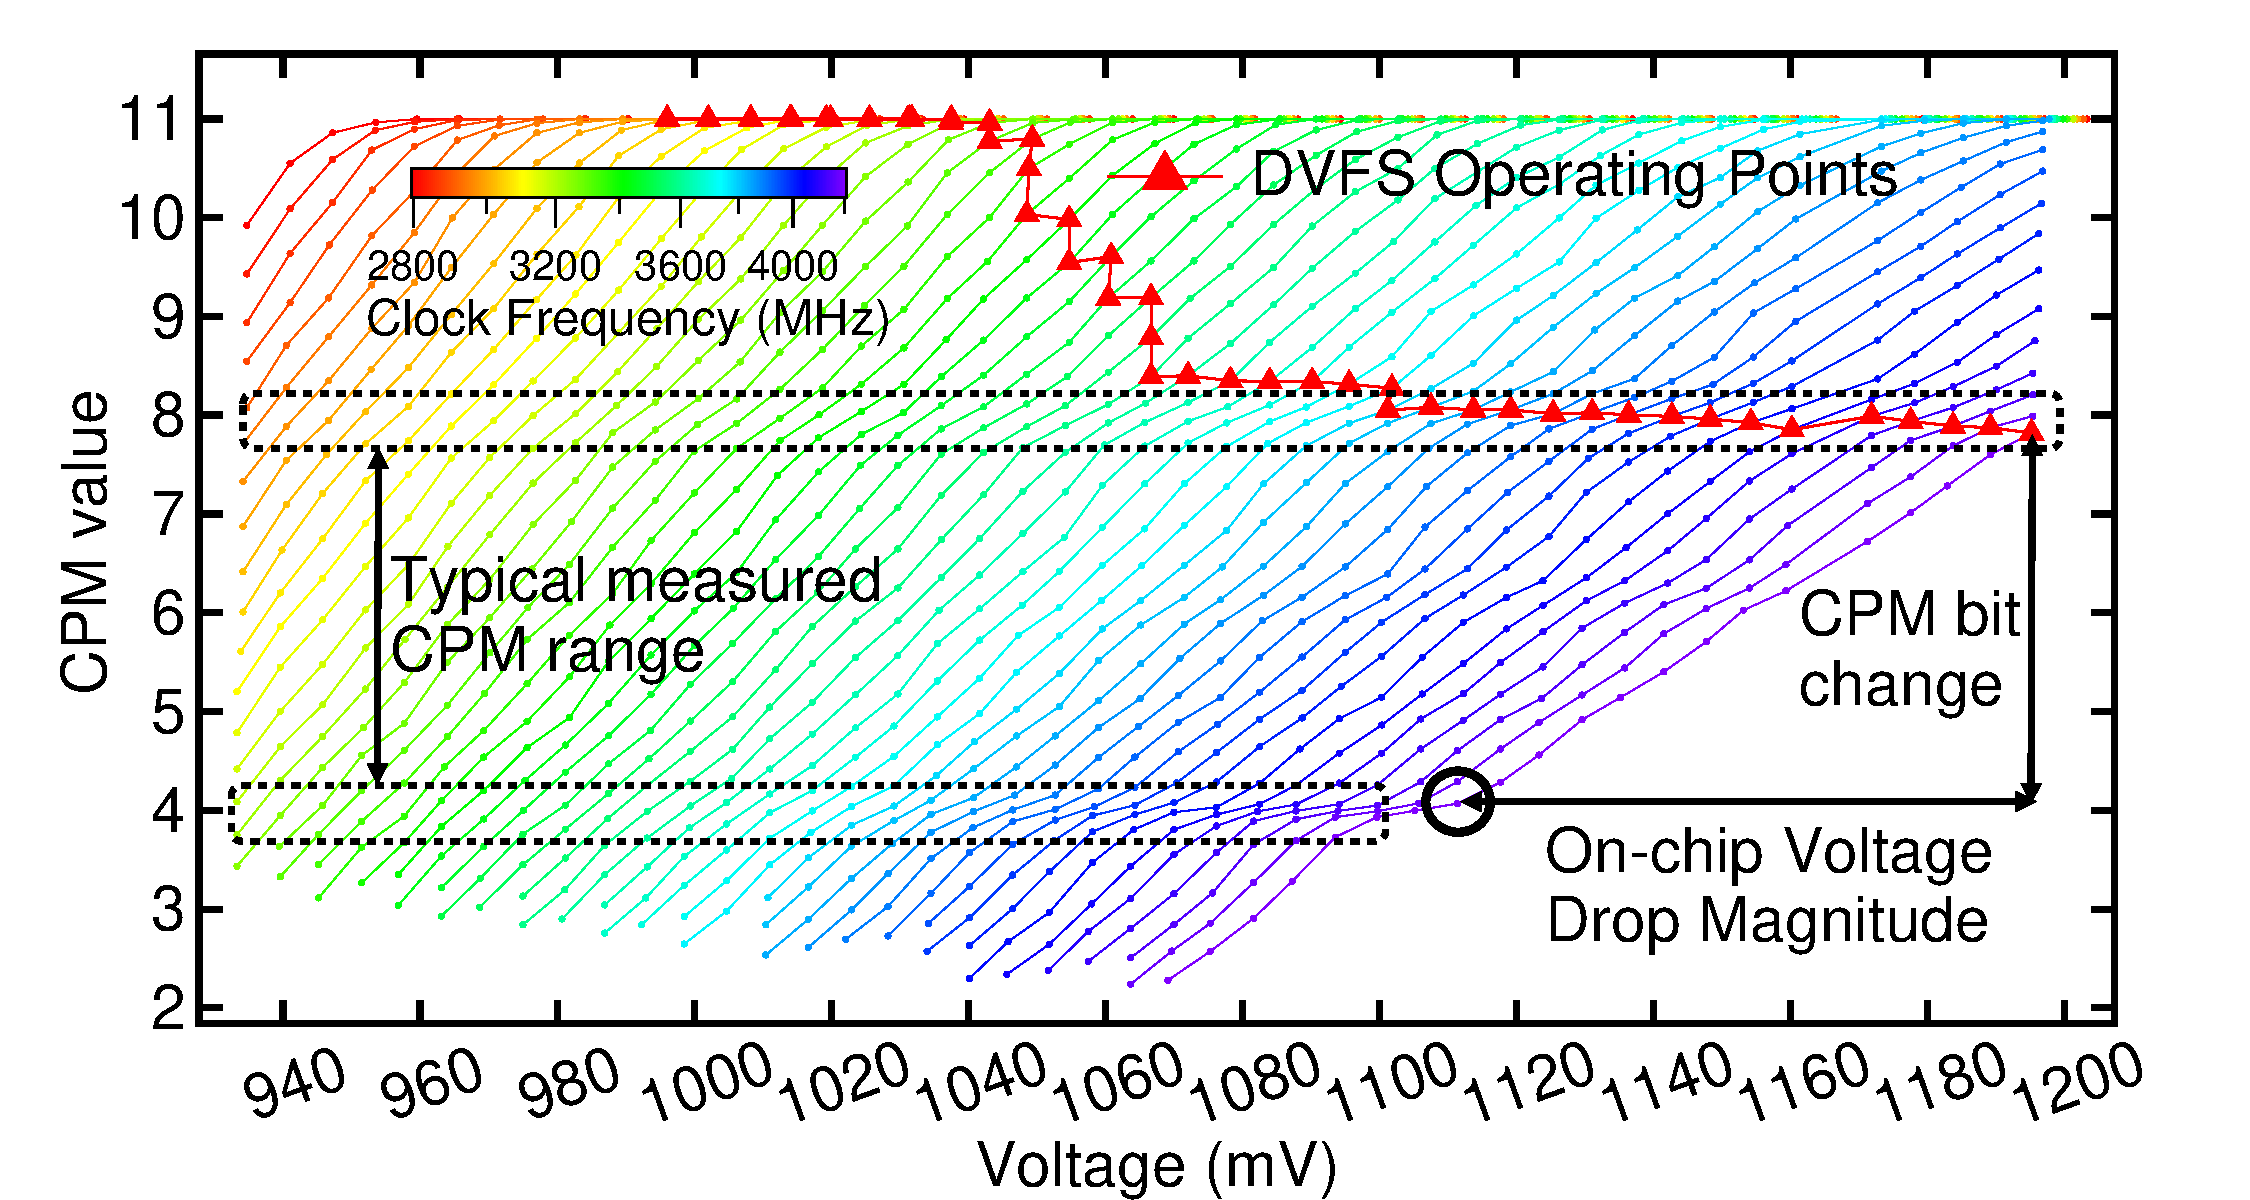
\includegraphics[trim=25 0 25 0,clip,width=0.425\linewidth]{graphs/voltage/cpm2volt.pdf}
      \label{fig:cpm2volt} 
  }
  \subfloat[The CPMs' sensitivity toward supply voltage in each core.] {
      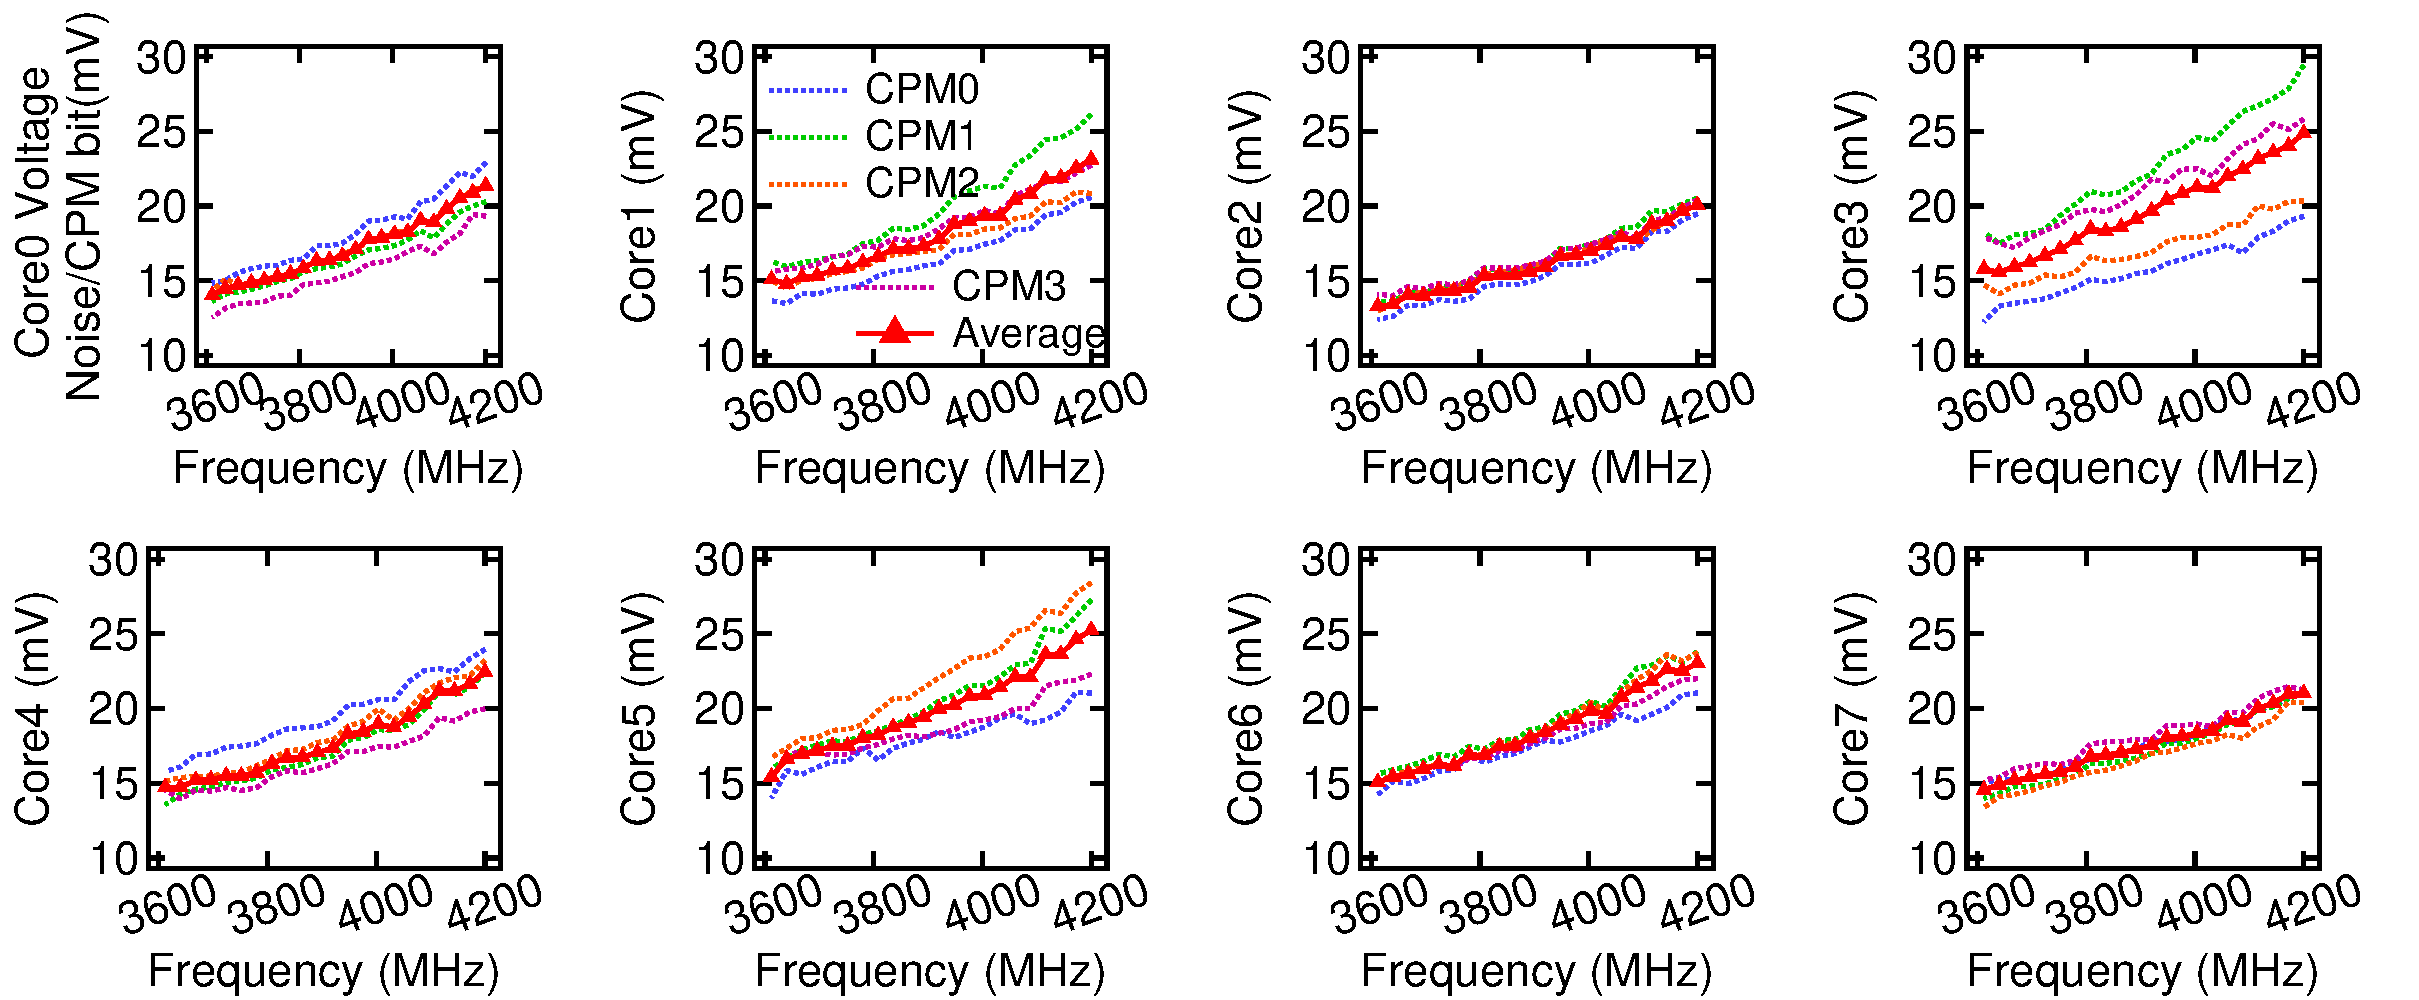
\includegraphics[trim=5 0 10 0,clip,width=0.575\linewidth]{graphs/voltage/cpm_process_variation.pdf}
      \label{fig:cpmsensitivity} 
  }
\caption{CPMs can sense the chip supply voltage with a precision of about 21mV per CPM bit at peak frequency.}
\label{fig:cpm-analysis}
\end{figure*}

We developed a novel approach to capture and characterize active timing margin's behavior using CPMs. We use CPM output to capture the on-chip voltage drop that affects the timing margin, which in turn affects the active timing margin's efficiency. In effect, we use CPMs as ``performance counters'' to estimate on-chip voltage, similar to how performance counters were first shown to be useful for predicting power consumption~\cite{isci2003runtime,huang2012accurate}.

Because timing margin is determined by on-chip voltage, capturing the CPM's output would reflect the transient voltage drops between the VRM output and on-chip voltage. Low on-chip voltage leads to less time for the CPM's synthetic-path edge to propagate through the inverter chain, and thus the CPM will yield a low output value. Under high on-chip voltage, the circuit runs faster, and the CPM yields a higher output.

To read the CPMs, we disable active timing margin because it dynamically adjusts the timing margin to keep the margin small and CPMs constant. The CPMs typically hover around an output value of 2 when active timing margin is active due to CPM calibration. By disabling active timing margin, we allow the CPMs' output values to ``float'' in response to on-chip voltage fluctuations, and thus we can study how supply voltage affects the behavior of CPMs. 

We use the IBM Automated Measurement of Systems for Temperature and Energy Reporting software (AMESTER)~\cite{floyd2011introducing} to read the CPMs' output. We record CPM readings under different on-chip voltage levels to determine how CPM responds to different on-chip voltage. AMESTER reads the CPMs at the minimal sampling interval of 32ms, which is restricted by the service processor. AMESTER can read the CPMs in either {\it sticky mode} or {\it sample mode}. In sticky mode, AMESTER reads the worst-case, i.e. smallest, output of each CPM during the past 32 ms, which is useful for quantifying worst-case droops. In sample mode, AMESTER provides a real-time sample of each CPM, which is useful for characterizing normal operation.

We use CPMs in sample mode to convert their output into on-chip voltage. To minimize experimental variability, we let the operating system run and throttle each core to fetch one instruction every 128 cycles. \Fig{fig:cpm-analysis} shows the mapping between CPM output and on-chip voltage. In~\Fig{fig:cpm2volt}, we sweep the voltage range for all possible clock frequencies and look at the average output of all 40 CPMs over 12,500 samples, which corresponds to about 1 minute of measurement. Each line corresponds to one frequency setting, and the system default voltage levels at DVFS operating points are highlighted with the marked line. Starting from 2.8~GHz, each diagonal line, as we move to the right, corresponds to a 28 MHz increase in frequency. The rightmost line corresponds to the peak frequency of 4.2~GHz. For any one frequency, the CPM value gets smaller as we lower the voltage, confirming the expected behavior that smaller voltages correspond to less timing margin. Also, for a fixed voltage ($x$-axis), higher frequency yields smaller CPM values ($y$-axis) because of less cycle time and a tighter timing margin. 

\begin{figure*}[t]
  \centering
  \hspace{-0.5cm}
  \begin{minipage}{0.5\linewidth}
    \centering
    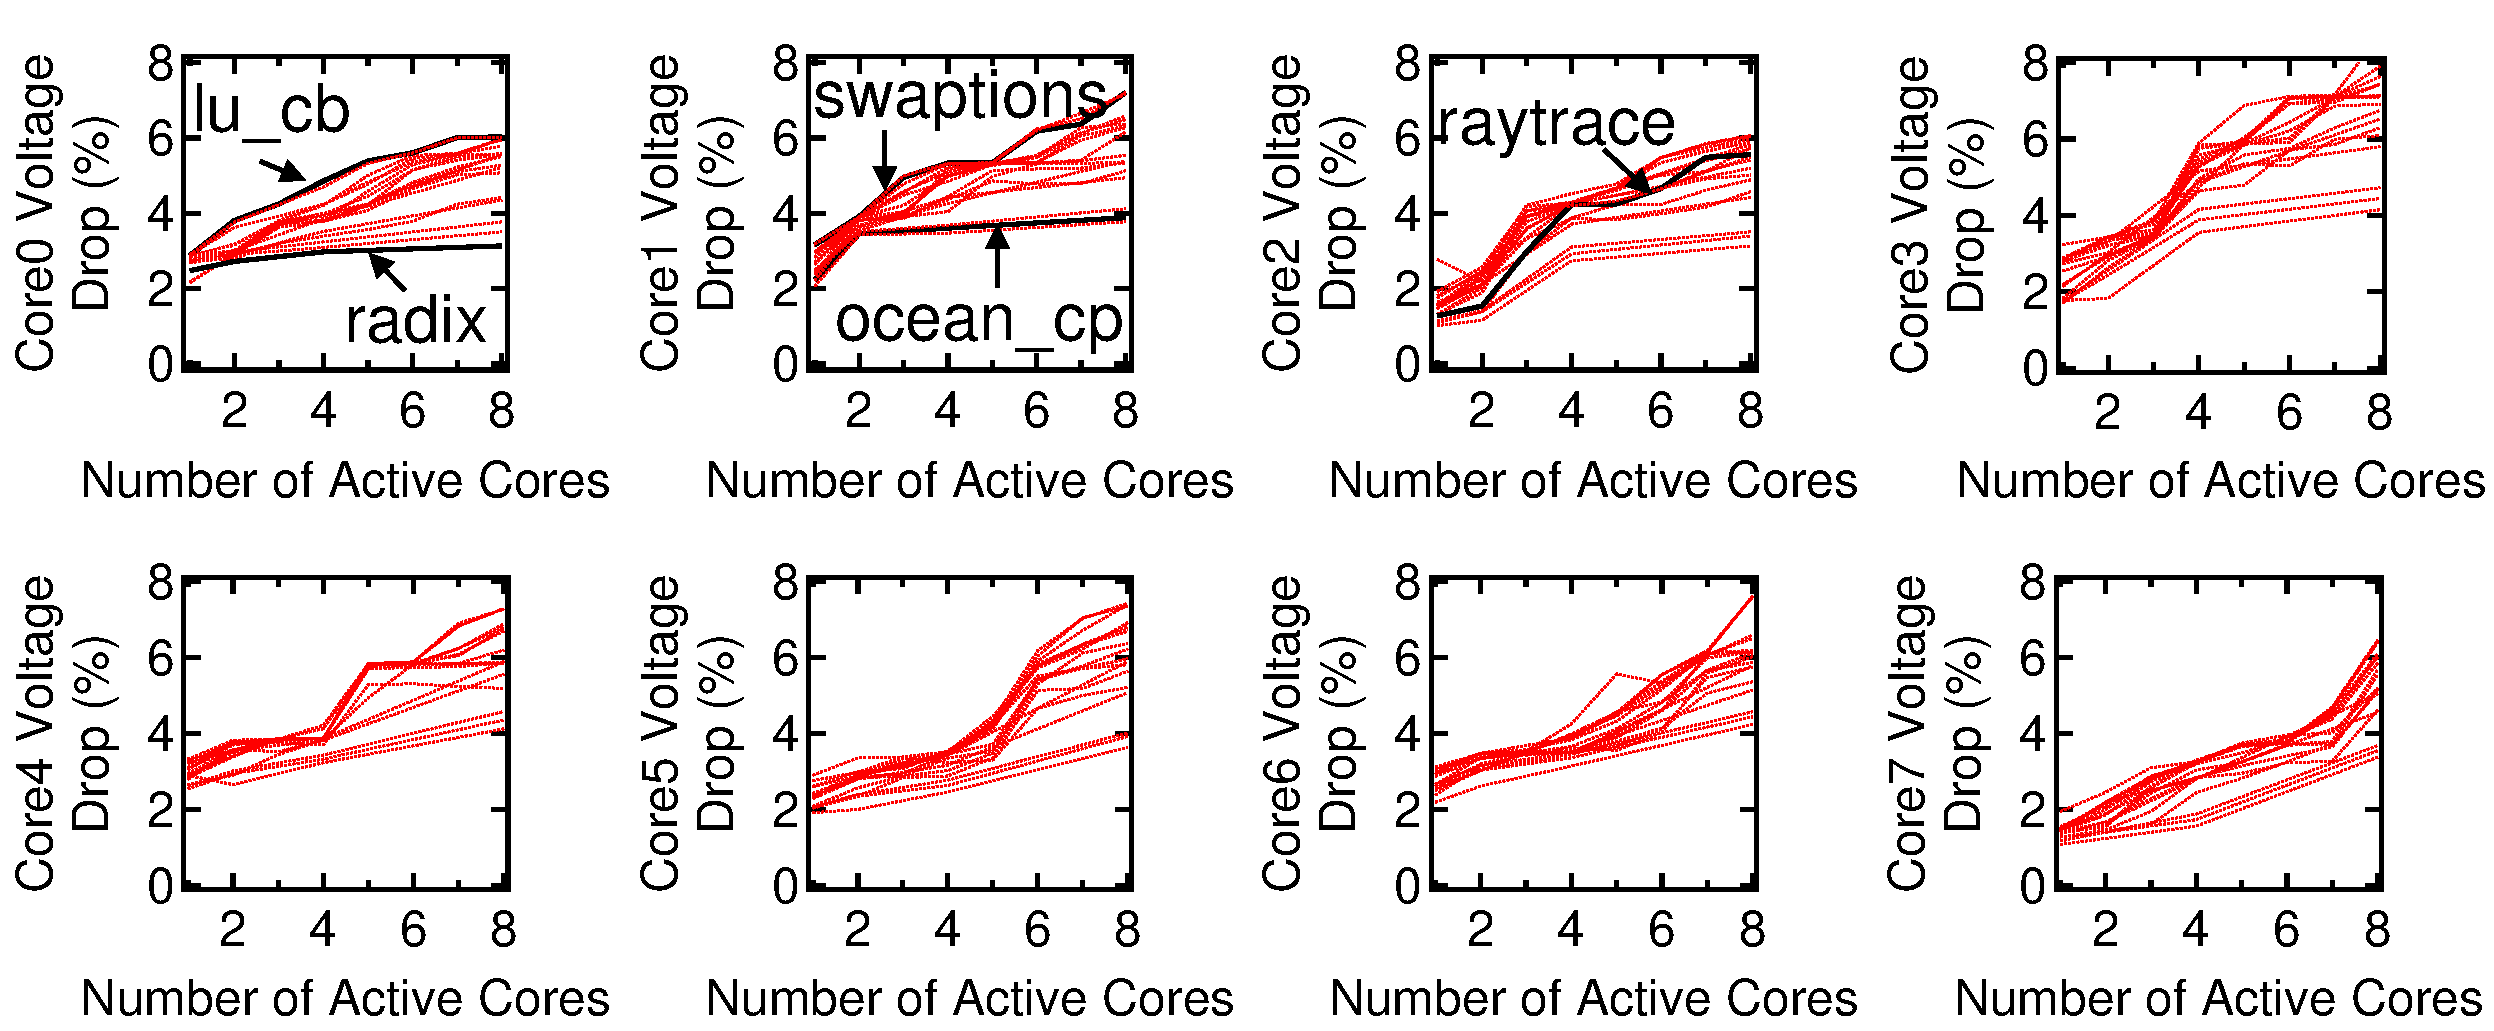
\includegraphics[trim=0 0 0 0,clip,height=1.5in]{graphs/voltage/cpm_scale_variation.pdf}
    \captionsetup{width=0.95\textwidth}
    \vspace{-0.2cm}
    \caption{On-chip voltage drop analysis across cores under different workloads.}
  \label{fig:cpm-variation} 
  \end{minipage}
\hspace{0cm}
  \begin{minipage}{0.47\linewidth}
    \centering
    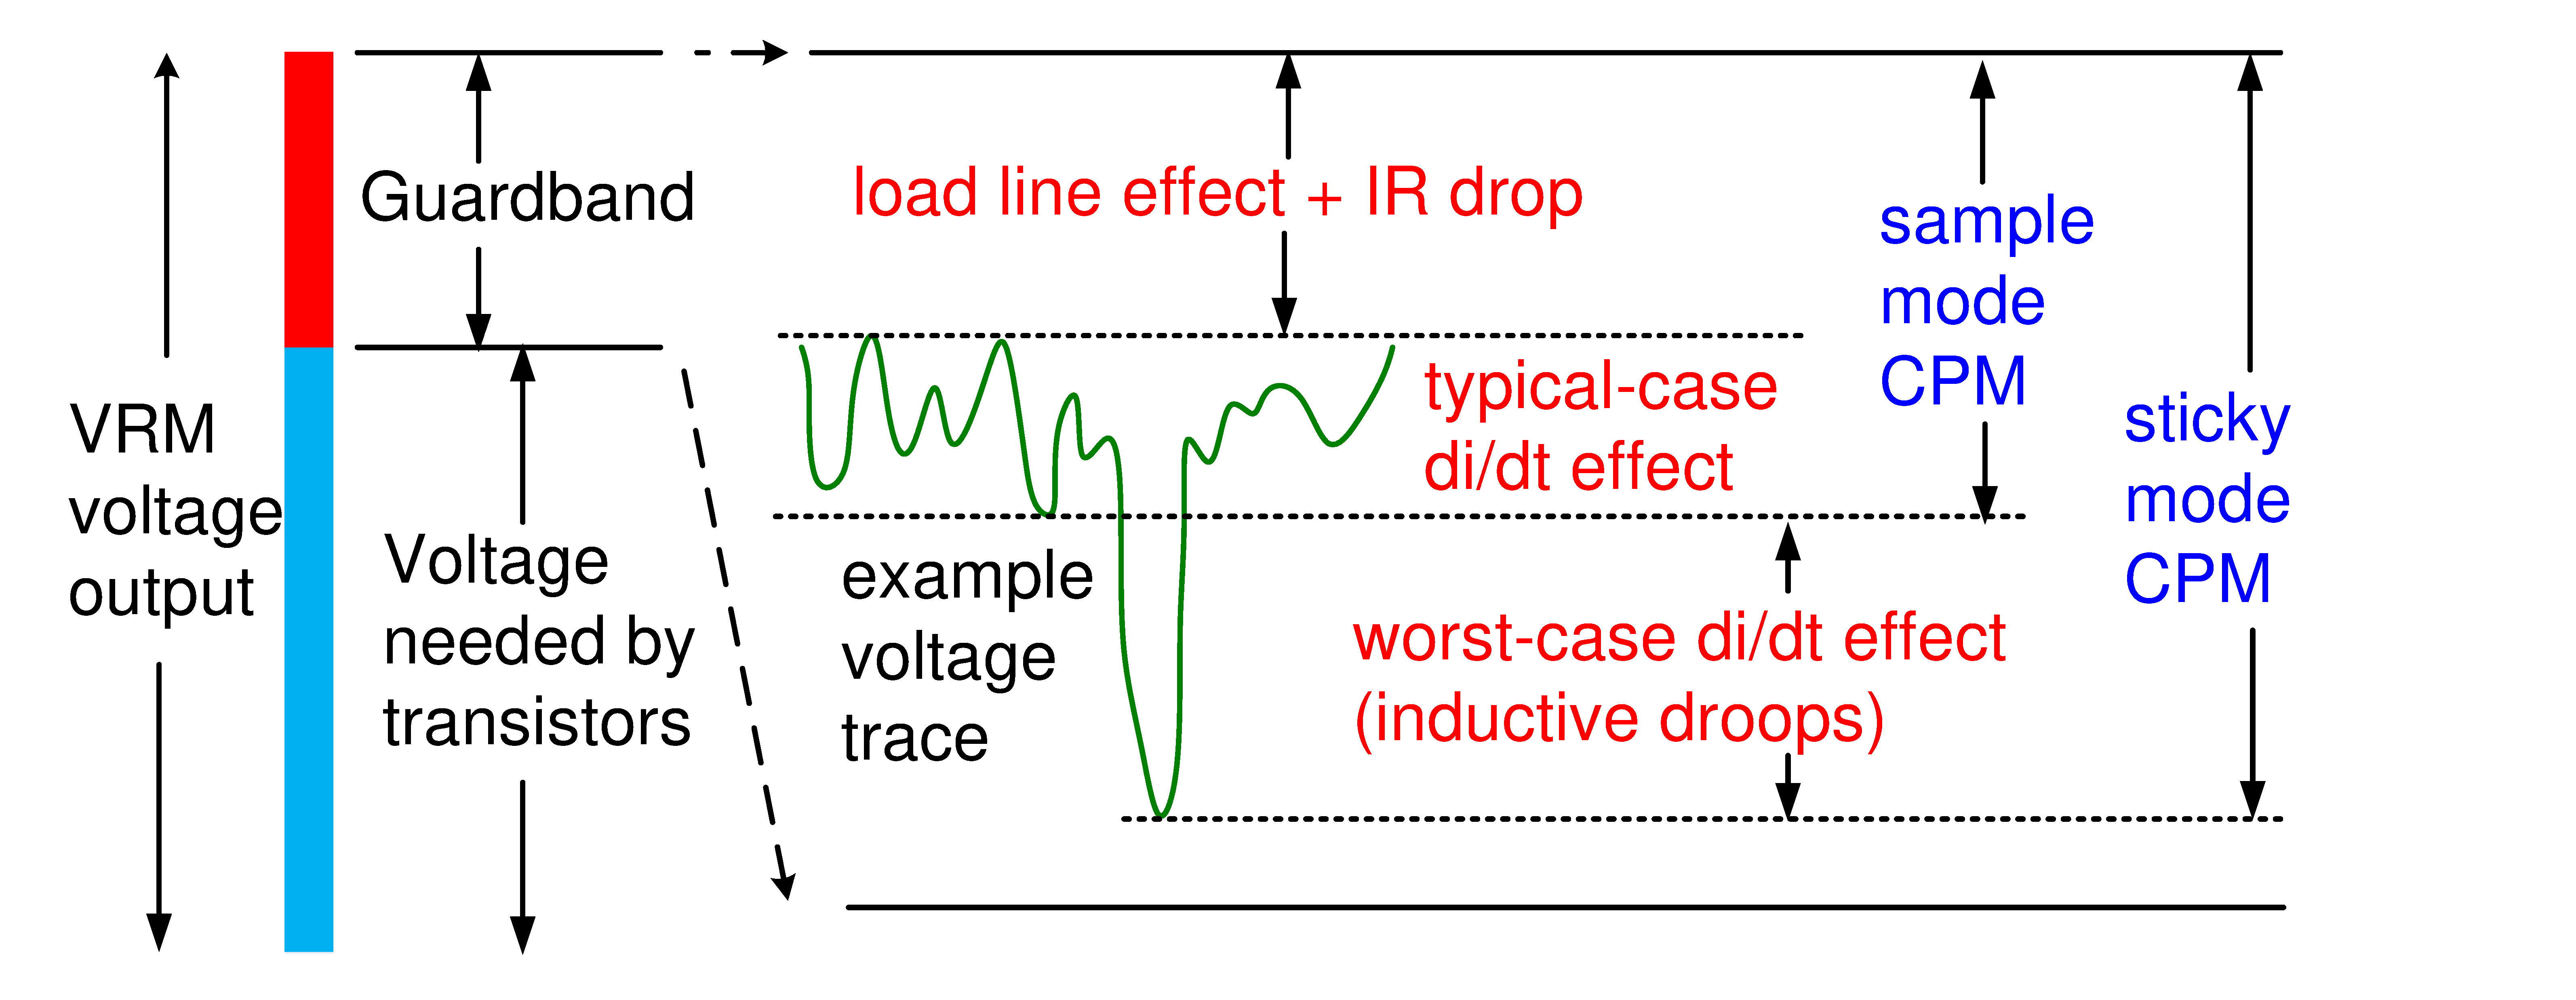
\includegraphics[trim=0 0 0 0,clip,height=1.5in]{graphs/voltage/noise_components.pdf}
    \captionsetup{width=0.95\textwidth}
    \vspace{-0.3cm}
    \caption{Voltage drop component analysis, including $di/dt$ droop, IR drop and the loadline effect.}
    \label{fig:vnoise-component} 
  \end{minipage}
\end{figure*}

\Fig{fig:cpm2volt} lets us establish a direct relationship between CPM and on-chip voltage. We observe a near-linear relationship between the two variables under each frequency. Therefore, with a linear fit, we can determine each CPM bit's significance. On average, one CPM output value corresponds to 21~mV of on-chip voltage. On this basis, we can estimate the magnitude of on-chip voltage drop during any 32~ms interval. For instance, if the measured CPM output drops from eight to four, the estimated on-chip voltage has dropped by 84~mV. 

\Fig{fig:cpmsensitivity} shows the sensitivity of the CPMs within each processor core. Although we see a near-linear relationship between frequency and all the CPMs, there is variation among the CPMs in each core and between cores. For instance, CPMs in Core~2,~6,~7 have steadier sensitivity compared to Core~1,~3,~5. The latter have higher distribution across CPMs. We attribute this behavior to process variation and CPM calibration error, as explained by prior work~\cite{floyd2013runtime}.

To ensure the robustness of our measurement results, we considered both repeatability and temperature effects. We repeated our experiment on another socket in the same server, and the result conforms to the same trend shown in~\Fig{fig:cpm2volt}. We observe that chip temperature varies between $27$\textdegree C at the lowest frequency to $38$\textdegree C at the highest. Internal benchmark runs show such temperature variation does not have significant influence over CPM readings, and thus we can draw general conclusions from~\Fig{fig:cpm2volt}.

\subsection{On-chip Voltage Drop Analysis}
\label{sec:voltage:rootcause:vdrop-analysis}

Using our on-chip voltage drop measurement setup, we quantify the magnitude of the on-chip voltage drop to explain the general core scaling trends seen in~\Sec{sec:characterization}. It is important to understand what factors, and more importantly how those factors, impact the efficiency of active timing margin as more cores are activated. 

\Fig{fig:cpm-variation} shows the measured results for the voltage drop across different cores within the processor, ranging from Core~0 through Core~7. The cores are spatially located in the same order as they appear on the physical processor~\cite{zyuban2013ibm}. The $y$-axis is the percentage of on-chip voltage drop from the nominal. Given the magnitude of voltage drop and knowledge about the system's nominal operating voltage, we can determine the percentage change. The $x$-axis indicates the total number of simultaneously active cores, specifically as they are activated in succession from core 0 to 7. Keeping consistent with \Fig{fig:workloadvariation}, each line in the subplots corresponds to one workload from PARSEC and SPLASH-2. Each subplot shows a particular core's characteristics with respect to every other (active or inactive) core in the processor. 

\Fig{fig:cpm-variation} lets us understand several important factors that affect active timing margin's efficiency. First, voltage drop increases as more cores are activated. For all workloads, voltage drop increases from about 2\% to 8\% as the number of active cores increases. The trend is similar to the diminishing benefits seen previously in the power and frequency improvement in \Fig{fig:workloadvariation}. As the magnitude of voltage drop increases, timing margin decreases and thus active timing margin's efficiency decreases at higher loads. 

\begin{figure*}[t]
     \subfloat[raytrace.] {
        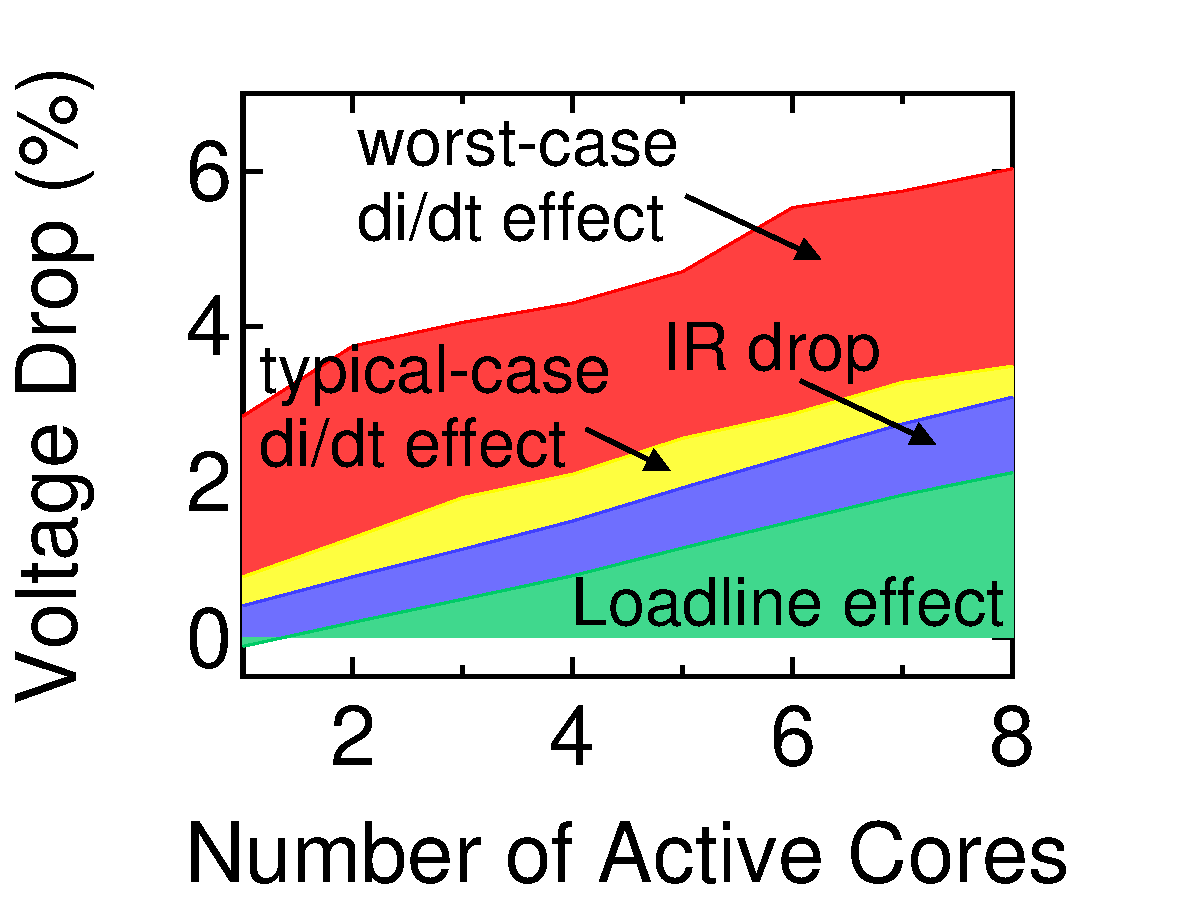
\includegraphics[trim=0 0 0 0,clip,width=.2\linewidth]{graphs/voltage/current_raytrace.pdf}
        \label{fig:raytrace_ir} 
      }
      \hspace*{-.1in}
      \subfloat[barnes.] {
        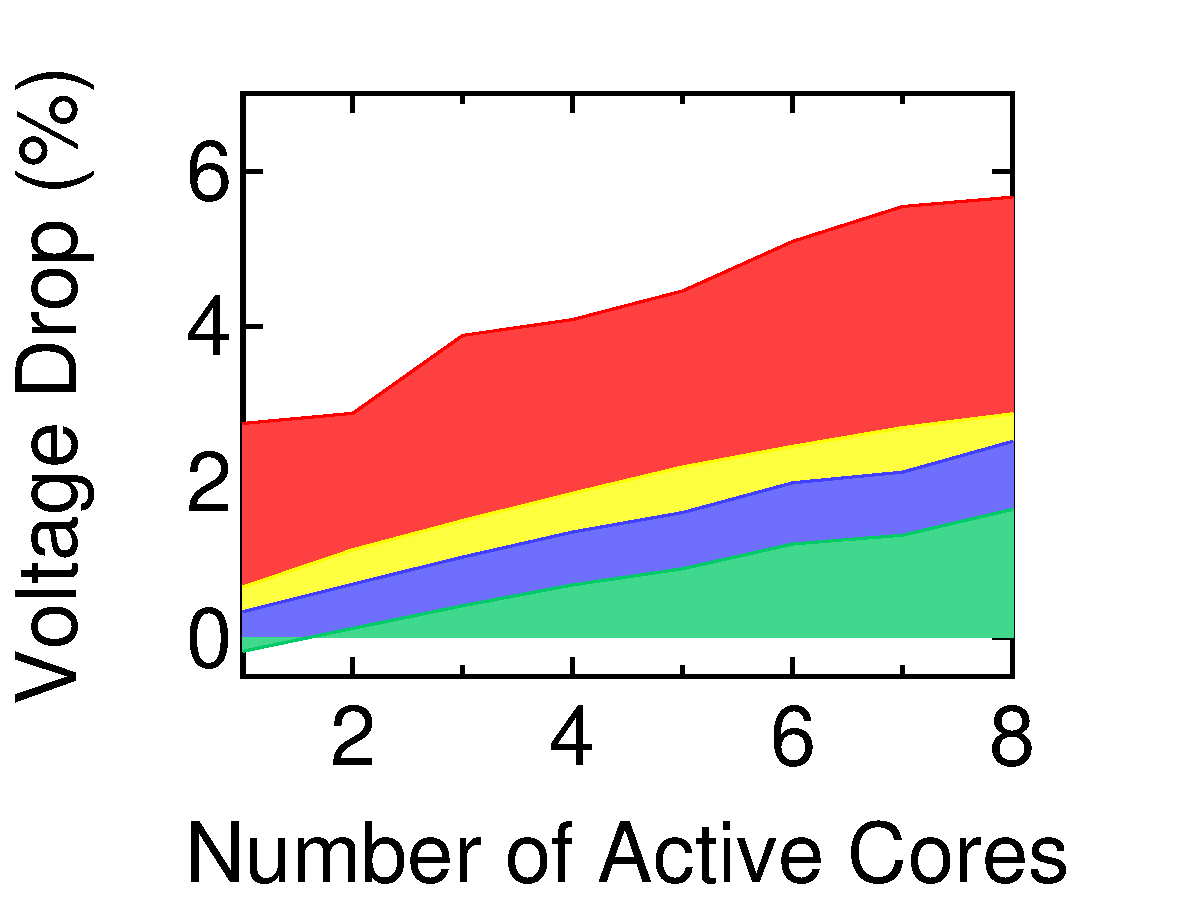
\includegraphics[trim=0 0 0 0,clip,width=.2\linewidth]{graphs/voltage/current_barnes.pdf}
        \label{fig:barnes_comp} 
      }
      \hspace*{-.1in}
      \subfloat[blackscholes.] {
        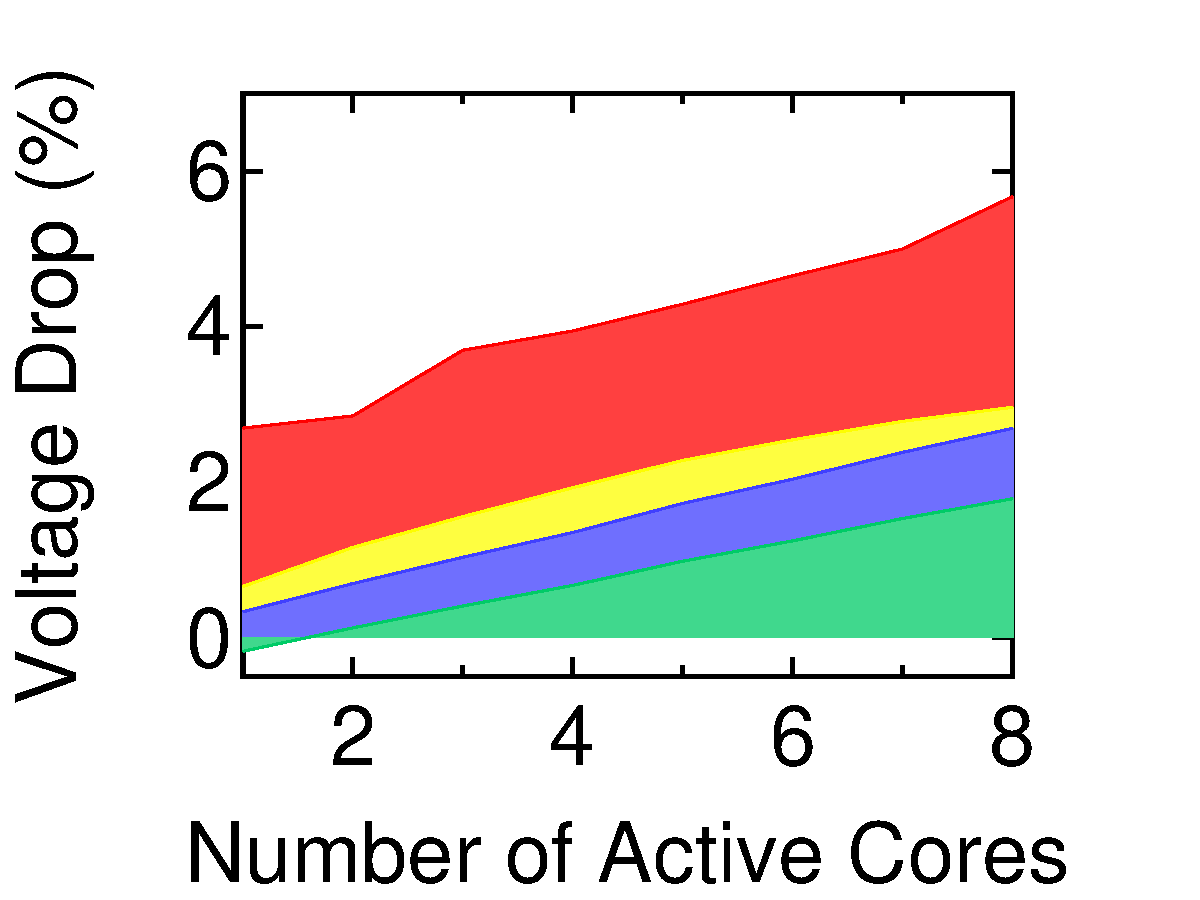
\includegraphics[trim=0 0 0 0,clip,width=.2\linewidth]{graphs/voltage/current_blackscholes.pdf}
        \label{fig:blackscholes_comp} 
      }
      \hspace*{-.1in}
      \subfloat[bodytrack.] {
        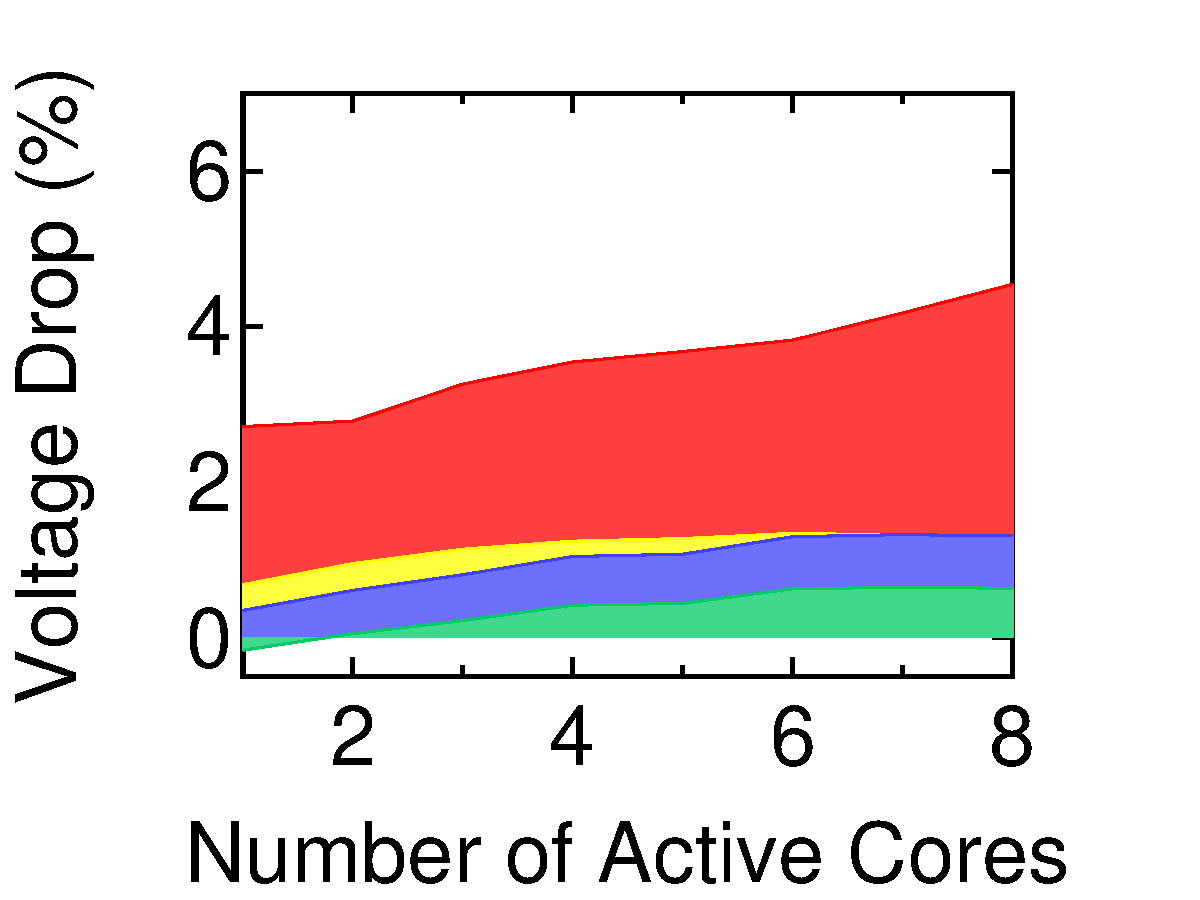
\includegraphics[trim=0 0 0 0,clip,width=.2\linewidth]{graphs/voltage/current_bodytrack.pdf}
        \label{fig:bodytrack_comp} 
      }
     \hspace*{-.1in}
      \subfloat[ferret.] {
        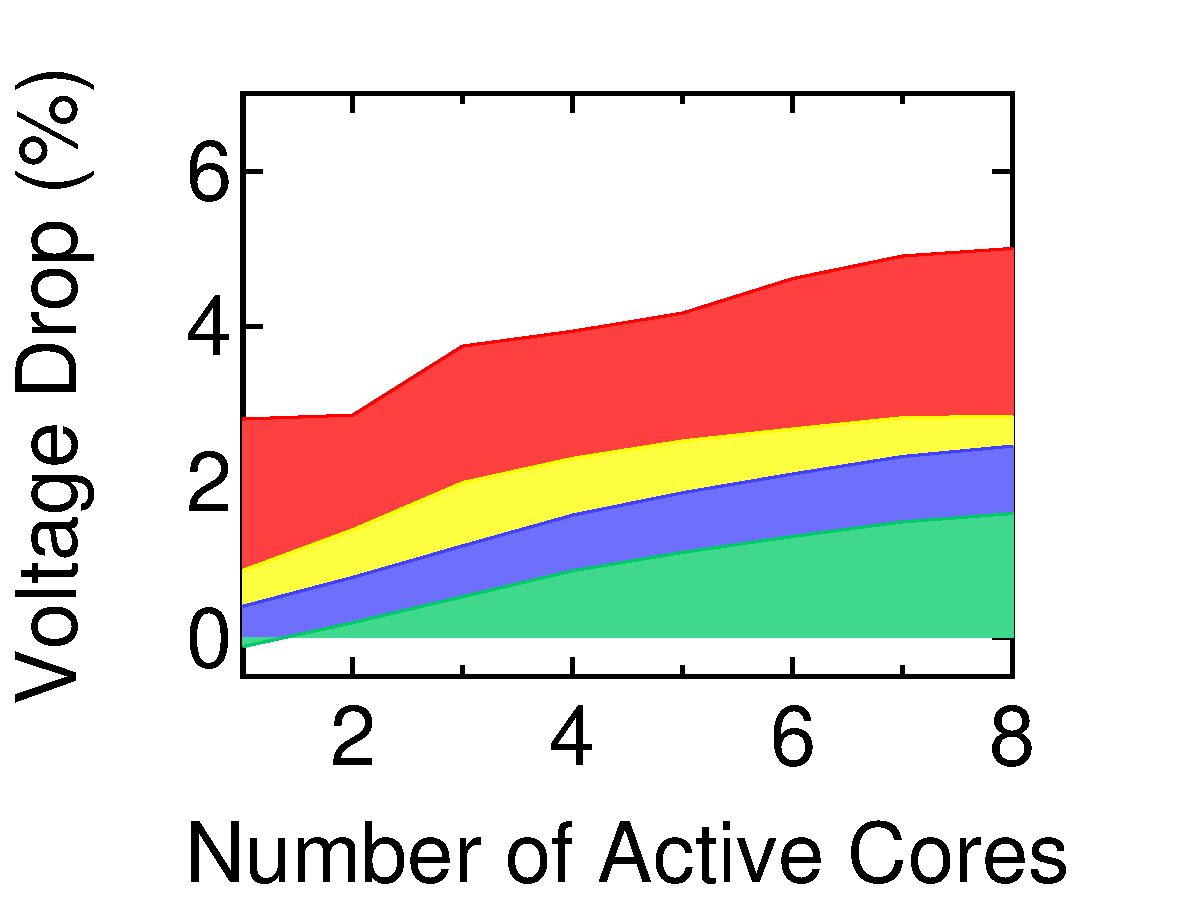
\includegraphics[trim=0 0 0 0,clip,width=.2\linewidth]{graphs/voltage/current_ferret.pdf}
        \label{fig:ferret_comp} 
      }
\vspace*{-.15in}
      \hspace*{-.05in} 
      \subfloat[lu\_ncb.] {
        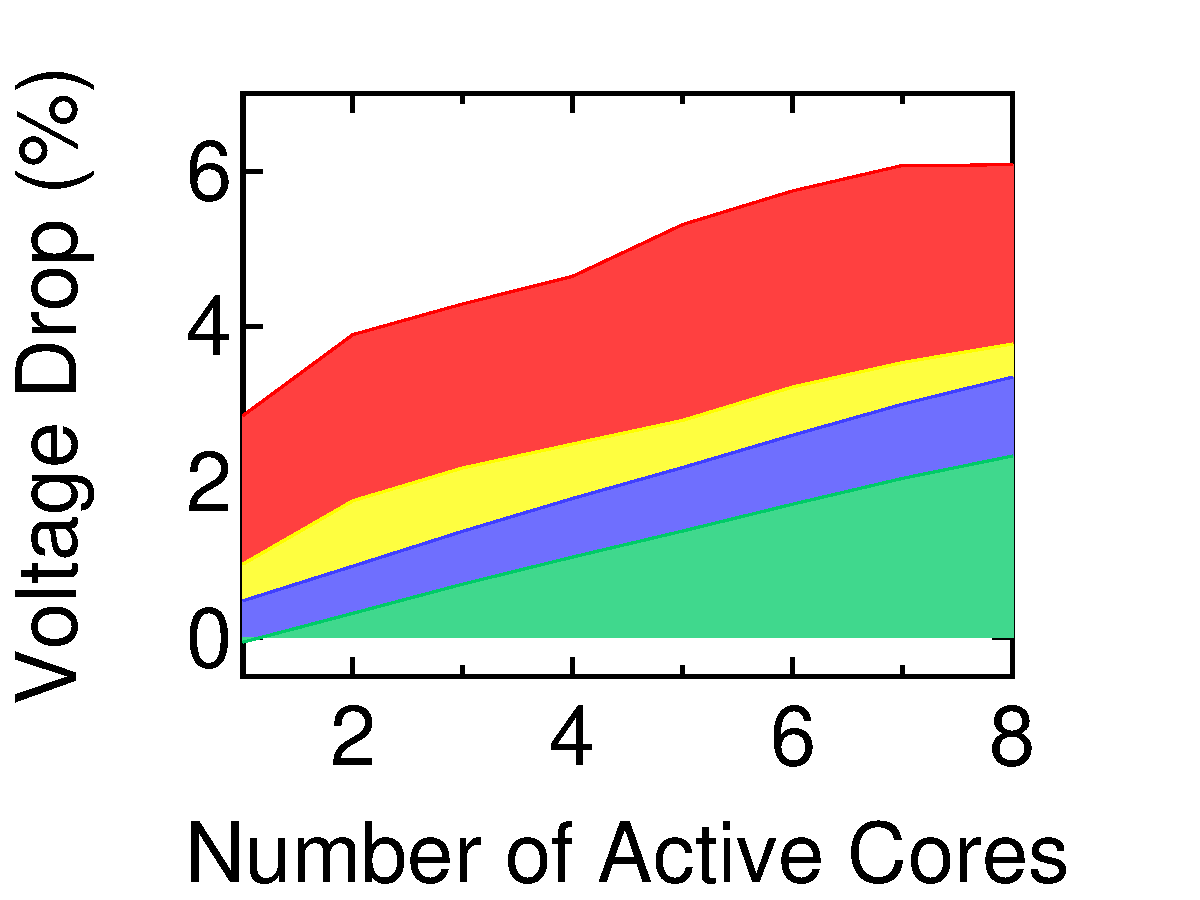
\includegraphics[trim=0 0 0 0,clip,width=.2\linewidth]{graphs/voltage/current_lu_ncb.pdf}
        \label{fig:lu_ncb_comp} 
      }
      \hspace*{-.1in} 
      \subfloat[ocean\_cp.] {
        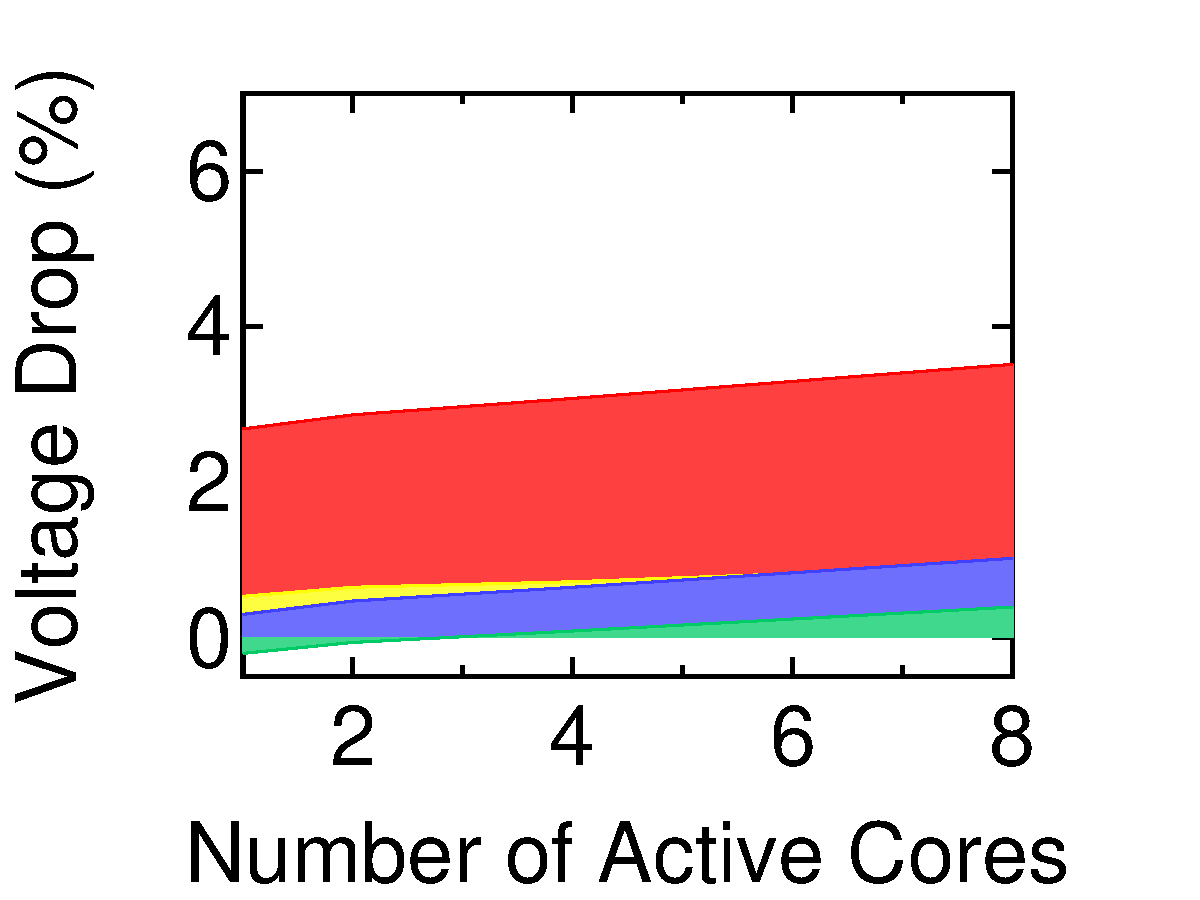
\includegraphics[trim=0 0 0 0,clip,width=.2\linewidth]{graphs/voltage/current_ocean_cp.pdf}
        \label{fig:ocean_cp_comp} 
      }
      \hspace*{-.1in} 
      \subfloat[swaptions.] {
        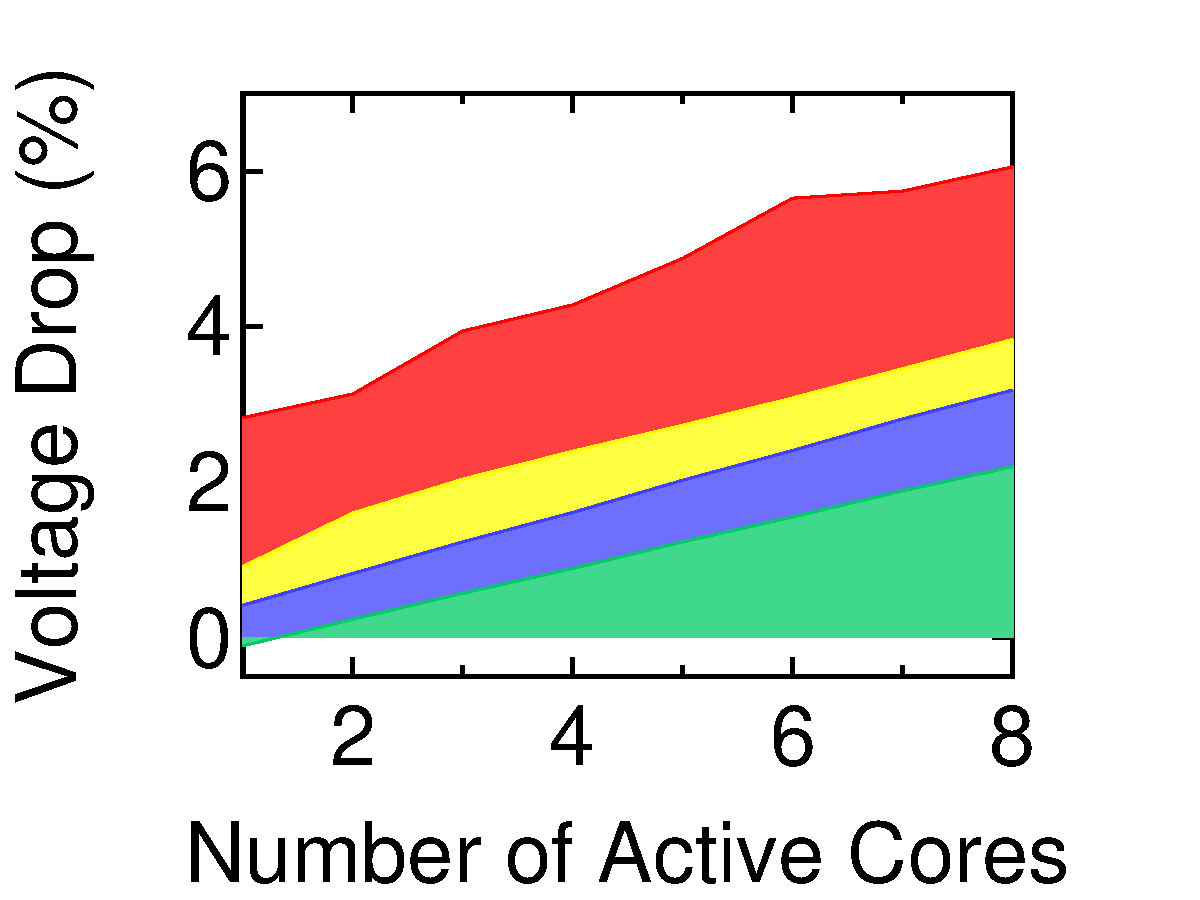
\includegraphics[trim=0 0 0 0,clip,width=.2\linewidth]{graphs/voltage/current_swaptions.pdf}
        \label{fig:swaptions_comp} 
      }
      \hspace*{-.1in} 
      \subfloat[vips.] {
        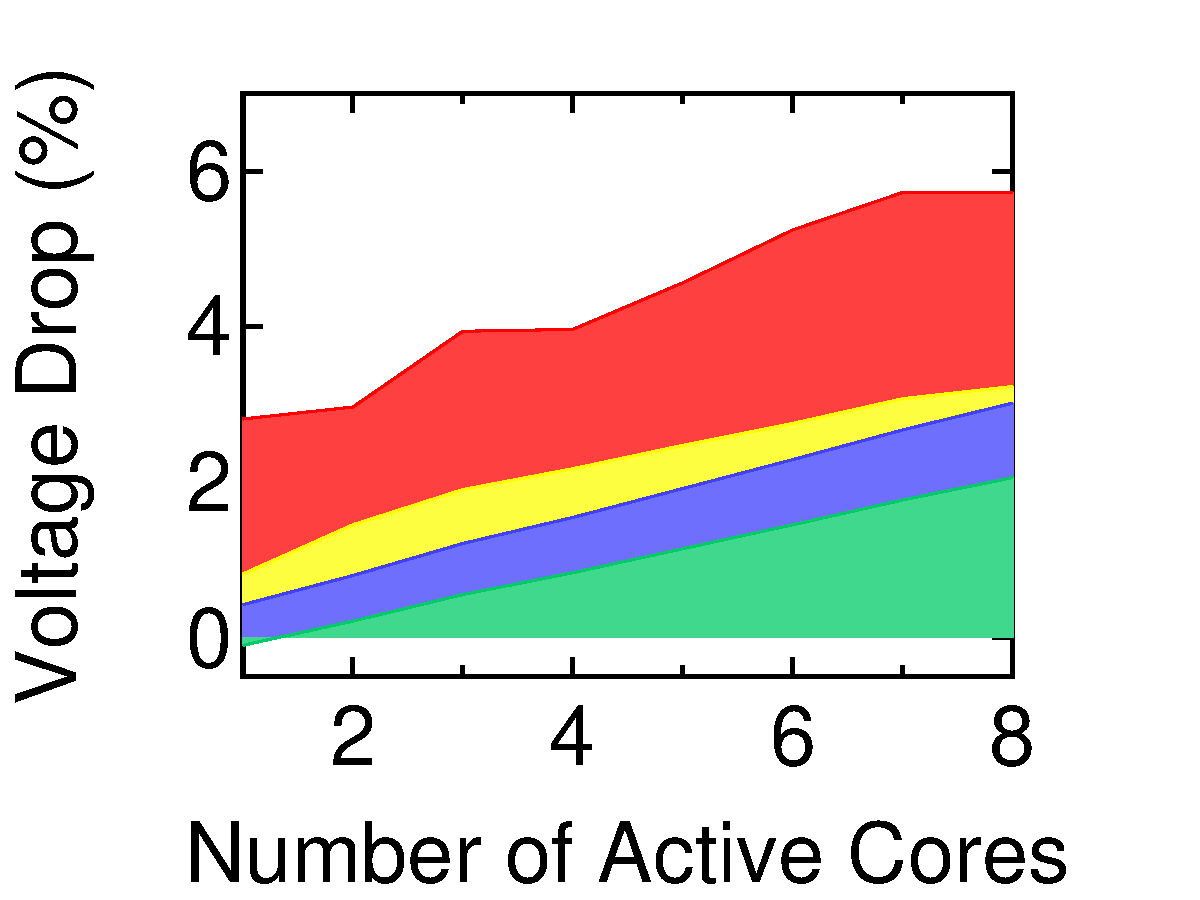
\includegraphics[trim=0 0 0 0,clip,width=.2\linewidth]{graphs/voltage/current_vips.pdf}
        \label{fig:vips_comp} 
      }
      \hspace*{-.1in} 
      \subfloat[water\_nsquared.] {
        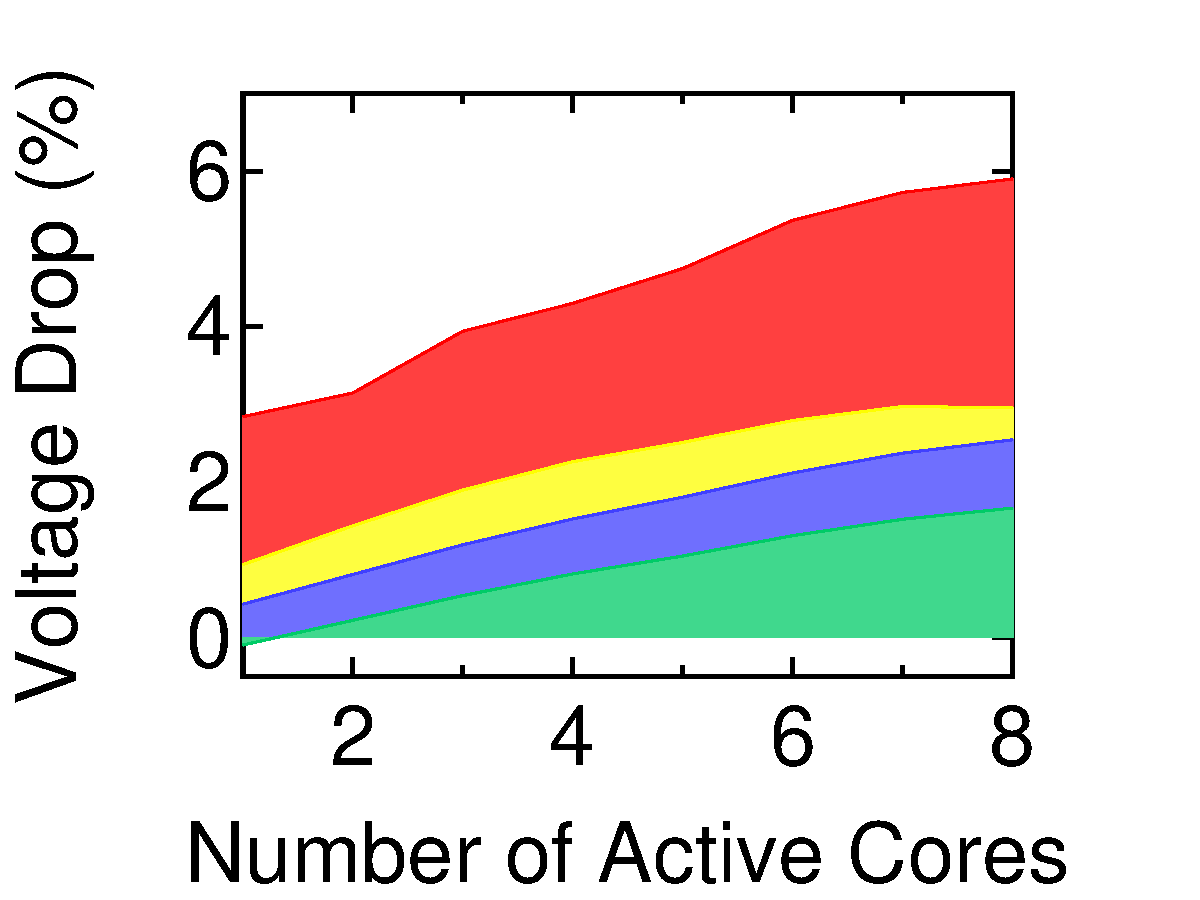
\includegraphics[trim=0 0 0 0,clip,width=.2\linewidth]{graphs/voltage/current_water_nsquared.pdf}
        \label{fig:water_nsquared_comp} 
      }
    \caption{Different components of on-chip voltage drop for some PARSEC and SPLASH-2 benchmarks. In general, as more of the processor's cores are activated, voltage drop increases by varying magnitudes across workloads.}
    \label{fig:drop-components} 
\end{figure*}

Second, the increasing on-chip voltage drop trend manifests as chip-wide global behavior because voltage drop affects all cores at the same time, regardless of whether they are idling or actively running a workload. For instance, when cores on the upper row (Core~0 through Core~3) are actively running a workload, they experience voltage drop. Meanwhile, cores in the bottom row also experience voltage drop even though Core~4 through Core~7 are not running any workloads. 

The implications of the second finding are that global effects, such as chip-wide $di/dt$ noise~\cite{gupta2007understanding,miller2012vrsync,bertran2014voltage} and off-chip IR drop, can affect active timing margin's system-wide power-saving efficiency because active timing margin makes decisions on the basis of the worst-case behavior of all cores. In particular, this behavior impacts the power-saving mode because the processor has a single off-chip VRM that will need to supply the highest voltage to match the most demanding core's voltage requirement. So, even if some cores are lightly active, the system may have to forgo their active timing margin benefits to support the activity of the busy core(s). In applications where workload imbalance exists, this can become a major efficiency impediment. 

Third, the on-chip voltage drop's scaling trend, as the number of active cores increases, tends to differ across cores, indicating that voltage drop has localized behavior in addition to the global behavior described previously. For instance, across all the cores the magnitude of voltage drop shifts upward significantly whenever that particular core is activated. For instance, Core~7's voltage drop increases by 2\% when it is activated, as evident in Core~7's voltage drop plot.

More generally, cores that are activated earlier have a higher voltage drop at first, and thereafter their voltage drop begins to saturate and plateau. For instance, Core~0 and Core~1 have a higher voltage drop when Core~0 through Core~3 are activated. These cores' voltage drop increase quickly when the number of active cores is less than four. On the contrary, the voltage drop for Core~4 through Core~7 does not change much while Core~0 through Core~3 are activated, but thereafter their voltage drop increases much more quickly.

Localized effects impact the operation of the per-core frequency-boosting mode. Each POWER7+ core has its own DPLL that can dynamically perform frequency scaling to improve performance when required. However, each core's performance can be boosted only when it is not affected by activity on its neighboring cores. In general, our observations imply that it is easier to boost clock frequency and, hopefully, performance -- at least for computing-bound workloads -- over reducing voltage, because frequency-boosting is largely affected by localized voltage drop. By comparison, the global voltage drop typically tends to have a more pronounced effect on the chip-wide power-saving mode. 

\subsection{Decomposing the On-chip Voltage Drop}
\label{sec:voltage:rootcause:vdrop-decompose}

To understand how workload heterogeneity affects the power-saving and frequency-boosting modes when all cores are active, we must understand why the on-chip voltage drop varies significantly from one workload to another with an increasing number of cores. For example, in \Fig{fig:cpm-variation} \benchmark{lu\_cb}'s voltage drop increases more quickly compared to \benchmark{radix}, whose voltage drop does not change much as the number of active cores increases.  We decompose the on-chip voltage drop into its three primary components (see \Fig{fig:vnoise-component}): worst-case $di/dt$ noise, also called voltage droops due to sudden current surges caused by microarchitecture activities; typical-case $di/dt$ noise due to regular current ripples; and passive voltage drop due to IR drop across the PDN and the loadline effect~\cite{lefurgy2011active} at the VRM.

We use a mixture of current sensing techniques and CPM measurements to decompose the voltage drop. To measure passive voltage drop (i.e., loadline effect + IR drop), we use VRM's current sensors. The IR drop and loadline effects are quantified using a heuristic equation verified against hardware measurements. The input to the equation is the current going from the VRM into the POWER7+ processor, sampled periodically.

We use CPMs to calculate the magnitude of typical and worst-case voltage noise. To get the typical $di/dt$ value, we run the CPMs in sample mode to acquire an immediate CPM reading, and after converting the CPM output into voltage, we subtract the passive component from it. To get the worst-case $di/dt$ value, we run the CPMs in sticky mode to acquire the largest voltage droop seen in the past 32~ms and subtract it from the long-term average measured in sample mode. 

We select several representative benchmarks from previously discussed data and decompose their on-chip voltage drop into $di/dt$ noise and passive drop in \Fig{fig:drop-components}. The subplots are in the form of a stacked area chart, showing the trend as more cores are progressively activated. Only Core~0 data simplifies the presentation of our analysis, although we have verified that the conclusions described in the following paragraphs hold true for the other cores as well.

By analyzing the data, we conclude that passive voltage drop, including IR drop across PDN and VRM's loadline is the dominant factor contributing to increasing voltage drop. Intuitively, these two passive effects have the most direct influence over active timing margin's behavior because they always exist steadily during execution as compared to $di/dt$ noise.

\begin{figure*}[t]
\centering
   \subfloat[] {
    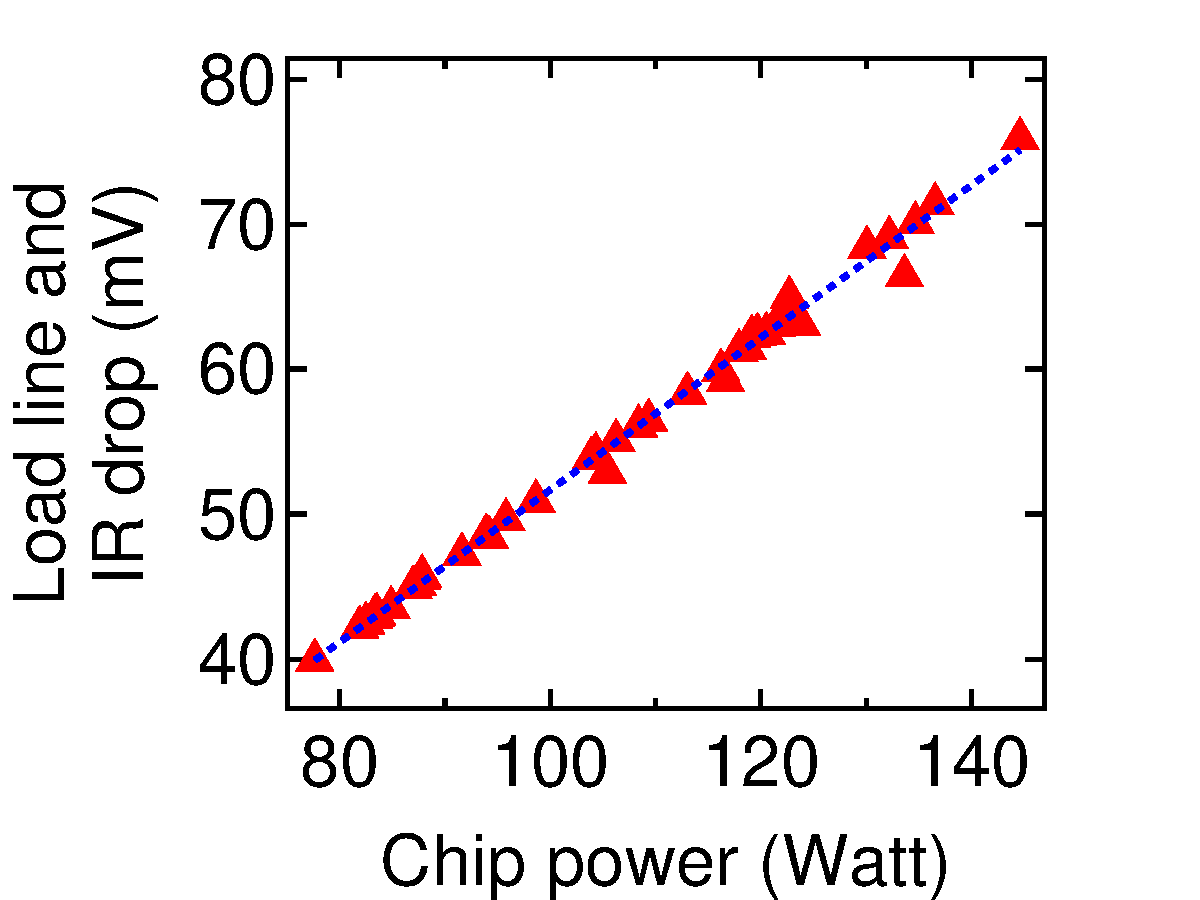
\includegraphics[trim=0 0 20 0,clip, height=1.25in]{graphs/voltage/pwr_loadline.pdf}
    \label{fig:pwr-loadline} 
  }
  \subfloat[] {
    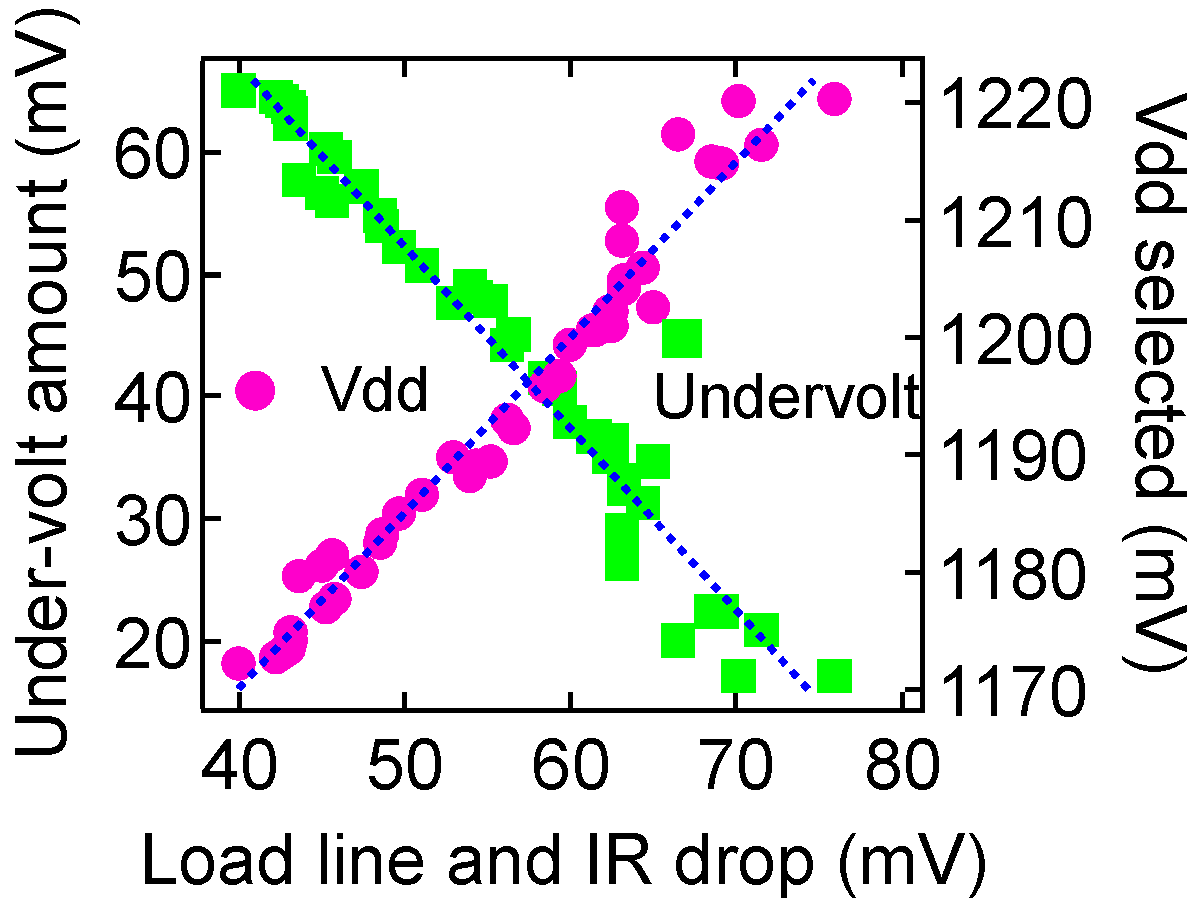
\includegraphics[trim=0 0 -50 0,clip,height=1.25in]{graphs/voltage/loadline_vdd.pdf}
    \label{fig:line-vdd} 
  }
  \subfloat[] {
    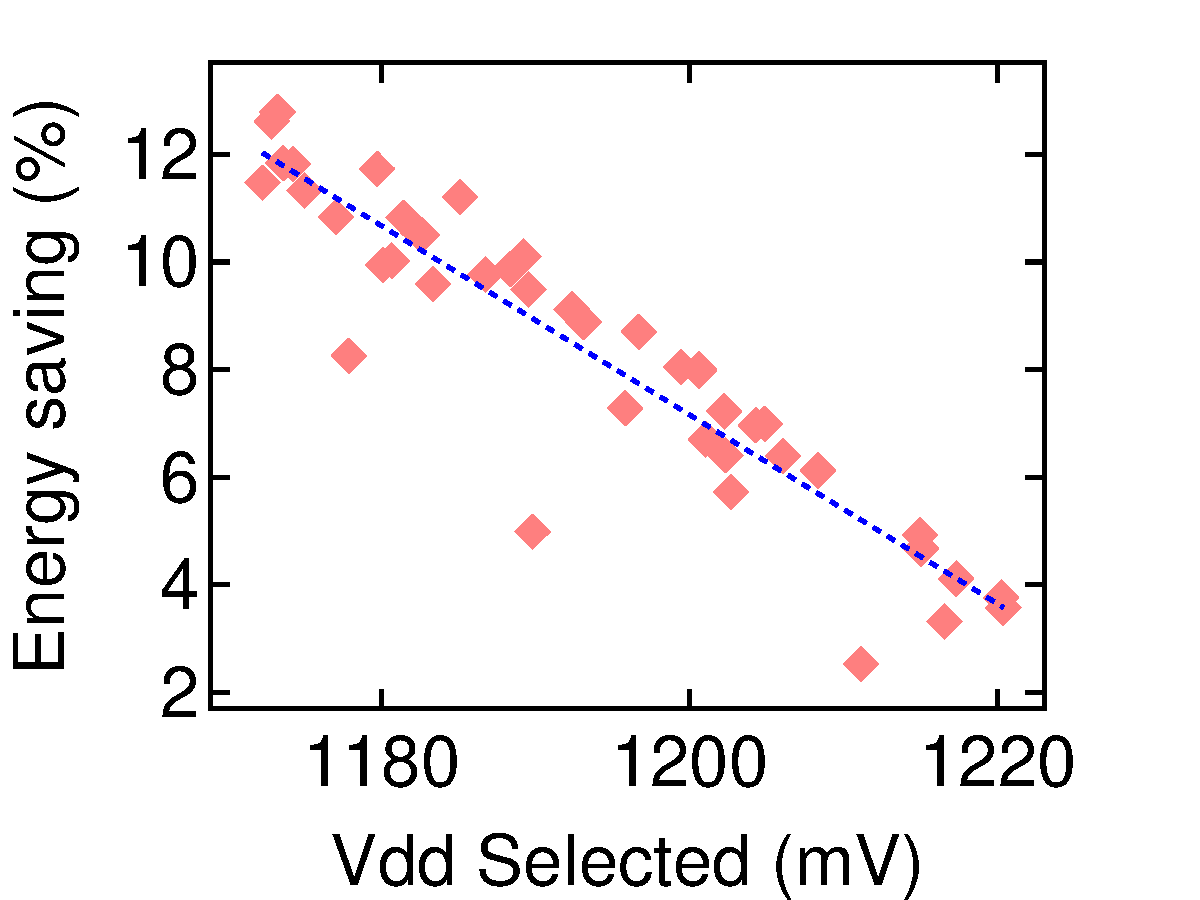
\includegraphics[trim=0 0 20 0,clip,height=1.25in]{graphs/voltage/vdd_saving.pdf}
    \label{fig:vdd-saving} 
  }
  \subfloat[] {
    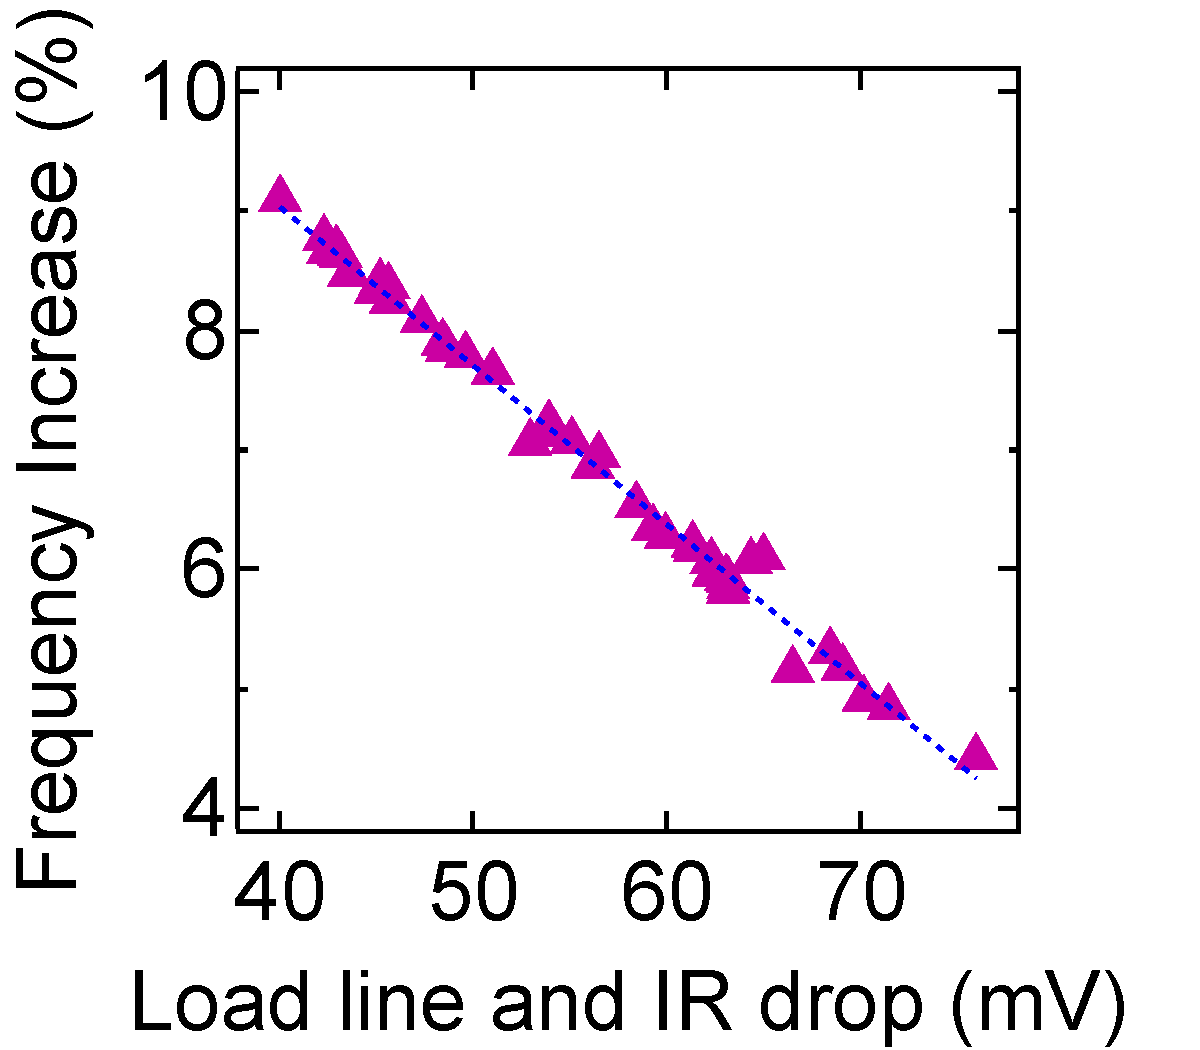
\includegraphics[trim=0 0 20 0,clip,height=1.25in]{graphs/voltage/loadline_freq.pdf}
    \label{fig:line-freq} 
  }
  \caption{Power-intensive workloads induce large loadline and IR drop, which severely limits the active timing margin system's undervolting capability, and thus impacts the system's overall power-saving potential.}
  \label{fig:ldir-proof}
\end{figure*}

As we scale the number of active cores, the worst-case $di/dt$ noise increases slightly across all of the benchmarks, and typical-case $di/dt$ noise decreases. For instance, the worst-case $di/dt$ noise growth is noticeable in \benchmark{bodytrack}, \benchmark{vips} and \benchmark{water\_nsquared}. When multiple cores are active simultaneously, they can have synchronous behavior, or random alignment, that can cause large and sudden current swings leading to voltage droops~\cite{reddi2010voltage,miller2012vrsync,kim2012audit}. However, our droop frequency analysis (not shown here) indicates that such large worst-case droops occur infrequently. On the contrary, typical-case $di/dt$ noise gets smaller when core count scales. With more active cores, microarchitectural activities stagger among different cores, which can lead to noise smoothing ~\cite{miller2012vrsync,reddi2010voltage}.

Compared to $di/dt$ noise, we find a clear scale-up trend of passive voltage drop from~\Fig{fig:drop-components}, and it contributes most to the scale-up of total voltage drop. IR drop and loadline effects increase almost linearly with the number of active cores because the passive voltage drop is caused by processor current draw, which is further determined by chip power. When more cores are used, the whole chip consumes more dynamic power and will lead to higher IR drop and loadline effects.

Because active timing margin can deal with occasional $di/dt$ voltage droops by slowing down frequency quickly, the rare voltage drop caused by this effect does not strongly influence the power-saving and frequency-boosting capability of active timing margin, even though they consume a significant portion of the total voltage guardband. Thus, we believe passive voltage drop is the main source of impact to active timing margin's efficiency. 

We confirm that loadline and IR drop cause active timing margin's inefficiency at full load by quantifying the relationship between their voltage drop under static guardbanding with respect to the system's two optimization modes: power saving (i.e., undervolting) and frequency boosting (i.e., overclocking). \Fig{fig:ldir-proof} shows the causal relationship between workload power consumption, loadline and IR drop, and the active timing margin's two modes. To ensure we have enough data points, we consider 27 SPECrate workloads on top of the existing 17 PARSEC and SPLASH-2 workloads used before. Each point represents the data we experimentally measured for one benchmark.

In~\Fig{fig:ldir-proof}, across all the subfigures, we see a strong correlation between passive voltage drop and the power-saving and frequency-boosting modes. \Fig{fig:pwr-loadline} shows a strong linear relationship between power and passive voltage drop. \Fig{fig:line-vdd} shows when a workload has a high loadline and IR drop, the voltage guardband is highly utilized, and so active timing margin has less room for undervolting. Thus, the voltage selected by active timing margin is higher. The result is fewer energy savings for high-power workloads, as the data in~\Fig{fig:vdd-saving} demonstrates. The same holds true for active timing margin's frequency-boosting mode. Here as well, a high loadline and IR drop reduce the timing margin; thus, the DPLL has limited room left to overclock the frequency as shown in \Fig{fig:line-freq}.

\section{Architecture \/ Scheduling Optimization}
\label{sec:voltage:opt}

We propose system-level scheduling techniques to improve the benefits of active timing margin. Our scheduler's overarching goal is to minimize the impact that loadline and IR drop have on an active timing margin processor's power and performance efficiency. We demonstrate \emph{active timing margin scheduling} (AMS) int \Sec{sec:voltage:opt:loadline}, and evaluates its effect in runtime power reduction in \Sec{sec:voltage:opt:result}

In a multi-socket server, conventional wisdom says to consolidate workloads onto fewer processors so that the idle processor can be shut down to eliminate wasted power~\cite{murthy2013linux,lo2014towards,leverich2014reconciling}. However, this principle does not apply to servers with active timing margin and per-core power-gating capability. Our measured results show consolidation actually leads to higher power o these systems. We propose loadline borrowing to maximize active timing margin's power-saving benefits for the underlying processors. Compared to workload consolidation, loadline borrowing achieves up to 12\% power savings.

\begin{figure}[!b]
\centering
\vspace*{-10pt}
\subfloat[Workload consolidation.] {
    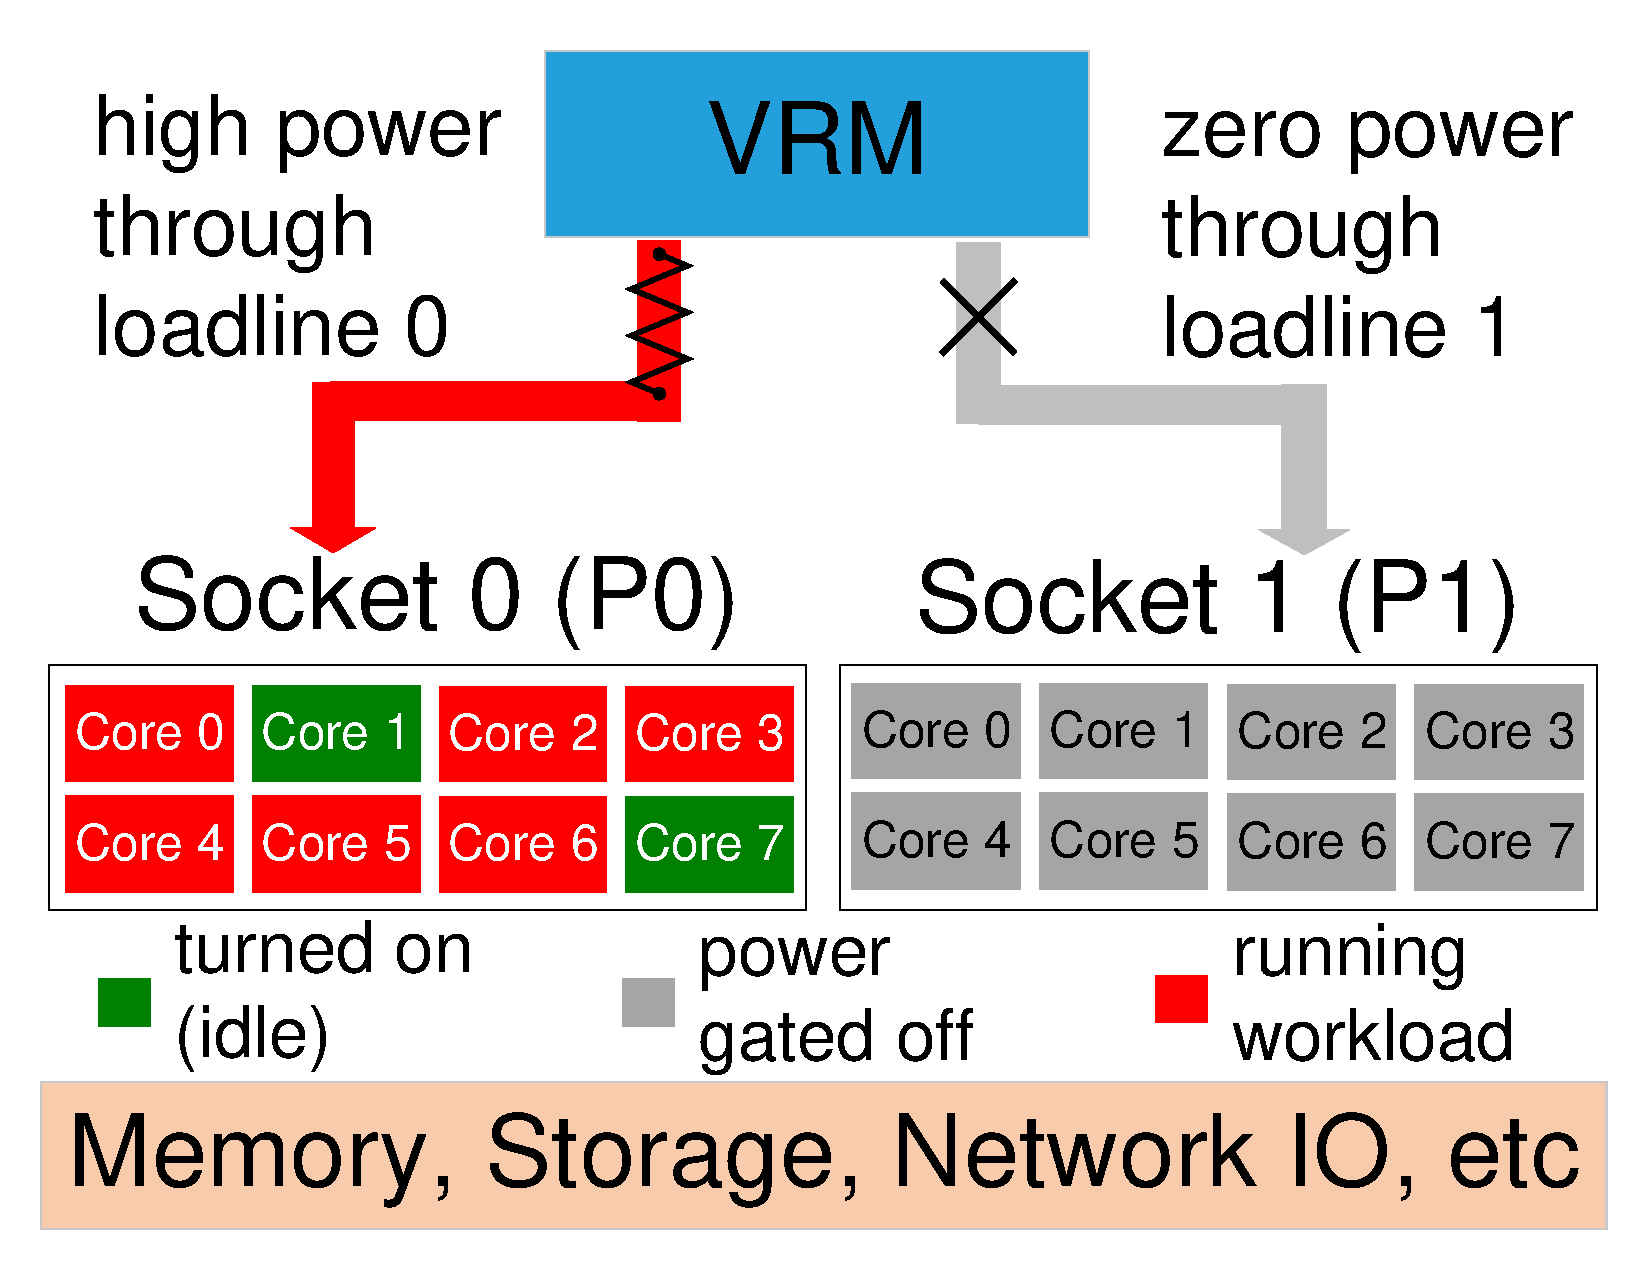
\includegraphics[trim=0 0 0 0,clip,width=.43\linewidth]{graphs/voltage/loadline-borrowing_diagram1.pdf}
    \label{fig:ll-borrow-idea1} 
}
\hfill
\subfloat[Loadline borrowing.] {
    \includegraphics[trim=0 0 0 0,clip,width=.43\linewidth]{graphs/voltage/loadline-borrowing_diagram2.pdf}
    \label{fig:ll-borrow-idea2} 
}
\caption{Loadline borrowing balances workloads across multiple sockets to reduce per-socket voltage drop and create room for active timing margin.}
%\vspace*{-0.4cm}
\label{fig:ll-borrow-idea}
\end{figure}

\subsection{Solution for Recovering Multicore Scaling Loss}
\label{sec:voltage:opt:loadline}

We use~\Fig{fig:ll-borrow-idea} to introduce how loadline borrowing optimizes workload distribution among a server's VRM-multiprocessor subsystem. In~\Fig{fig:ll-borrow-idea}, multiple processor sockets share a common VRM chip, each with its own power delivery path from the VRM to the die. The VRM can generate multiple V$_{dd}$ levels for different processors, which is normal for contemporary systems. In the following discussion, we use~\Fig{fig:ll-borrow-idea1} and \Fig{fig:ll-borrow-idea2} to analyze the scenarios of workload consolidation and loadline borrowing and highlight the necessity of considering VRM's role in systems with active timing margin processors. Other components such as memory chips and disks are powered on steadily throughout our analysis.

\Fig{fig:ll-borrow-idea1} shows a traditional consolidation schedule for a multisocket server. Workloads are all mapped to socket 0 so that socket 1 can be shut down. Because all power goes to socket 0, the passive voltage drop along the power-delivery path from VRM to processor 0 is very high, which limits active timing margin's potential to undervolt.

Loadline borrowing balances workloads equally among all available sockets, and power gates off unneeded cores to eliminate idle power consumption.~\Fig{fig:ll-borrow-idea2} illustrates a loadline-borrowing schedule. In~\Fig{fig:ll-borrow-idea2} active cores are distributed to each socket evenly, and each socket power gates off a set of unused cores to achieve the same idle power elimination effect as in a consolidated schedule. In this schedule, each socket draws less power, reducing the passive voltage drop each processor experiences. This allows active timing margin to reduce more voltage from each processor and hence improve total processor power.

We use our two-socket platform to illustrate the benefits of loadline borrowing. We compare the case of conventional workload consolidation, which places all loaded cores on one processor as the baseline, to loadline borrowing, which balances the loaded core count across both processors. We keep eight of the total 16 cores turned on to respond instantly to utilization levels of up to 50\%. The remaining eight cores are assumed to be not instantly needed, and therefore are put into a deep sleep (power-gated) state. We run the workload using one to eight cores. In the conventional case, all of the turned-on cores reside on a single processor. In the loadline borrowing case, each processor has four cores that are turned on and active. In either case, we measure and compare the two processors' total chip power.

\begin{figure}[t]
\centering
\vspace*{-10pt}
\subfloat[Undervolt scaling.] {
    \includegraphics[trim=0 0 65 0,clip,width=.43\linewidth]{graphs/voltage/raytrace_split_uv.pdf}
    \label{fig:split_raytrace_uv} 
}
\hfill
\subfloat[Power scaling.] {
    \includegraphics[trim=0 0 65 0,clip,width=.43\linewidth]{graphs/voltage/raytrace_split_pwr.pdf}
    \label{fig:split_raytrace_pwr} 
}
\caption{Distributing \benchmark{raytrace} across two processors reduces passive voltage drop, allowing more power saving under high core count.}
\vspace{-0.4cm}
\label{fig:split_raytrace}
\end{figure}

As an example, \Fig{fig:split_raytrace} shows the results for \benchmark{raytrace} with loadline borrowing. \Fig{fig:split_raytrace_uv} shows that loadline borrowing offers a better undervolting benefit no matter how many cores are used. There are two reasons. First, loadline borrowing lets each processor power on fewer cores, which cuts down leakage power, and thus substantially reduces the idle power. For~\benchmark{raytrace}, less idle power gives 20mV more undervolting benefit when one core is active. Second, balancing application activity (threads) and system requirements (idle cores) across the processors' loadline distributes dynamic power across each processor, which further reduces the passive drop for each processor. When eight cores are active, reduced dynamic power allows an additional 20mV reduction. 

\Fig{fig:split_raytrace_pwr} shows loadline borrowing can reduce a significant amount of total chip V$_{dd}$ power. The biggest effect is achieved when more cores are used. In~\Fig{fig:split_raytrace_pwr} loadline borrowing reduces power consumption by 1.6\%, 4.2\% and 8.5\% when two, four and eight cores are used, respectively. The result is intuitive because each processor's passive voltage drop is reduced when fewer cores are active. Thus, distributing the workload when more cores are active yields larger benefits. 

Loadline-borrowing is suitable only for workload scheduling within a multisocket server. In this setting, all other resources, such as memory, disk and network I/O, remain active when workloads are consolidated onto a few processors. When workloads are consolidated across multiple servers, the idle power reduction from turning off the used memory and hard drive outweighs active timing margin's processor power savings. In this case, the scheduler will consolidate workloads onto fewer servers first, then on each server loadline borrowing can be used to further improve cluster power consumption. We leave this discussion to future studies.

\subsection{Power Reduction Improvement}
\label{sec:voltage:opt:result}

\begin{figure}[t]
\centering
    \includegraphics[trim=0 0 0 0, clip,width=0.8\linewidth]{graphs/voltage/loadline-borrowing_scale.pdf}
    \caption{Loadline borrowing's power and energy improvement under different numbers of active cores. Compared to the baseline, loadline borrowing consistently shifts up every workload's power improvement.}
    \label{fig:ll-borrow-scale}
    \vspace{-0.2cm}
\end{figure}

\begin{figure*}[t]
\centering
    \vspace{0.4in}
    \includegraphics[trim=0 0 0 0,clip,width=\linewidth]{graphs/voltage/split_benefits_all.pdf}
    \caption{Loadline borrowing's power and energy improvement when eight cores are active.}
    \label{fig:ll-borrow-8core-normal}
\end{figure*}

Current operating systems are unaware and do not incorporate loadline knowledge into process scheduling. We use the Linux kernel's taskset affinity mechanism to emulate a schedule that dynamically performs loadline borrowing. We evaluate loadline borrowing on a wider set of benchmarks including all of PARSEC and SPLASH-2 workloads to capture the general trends. Briefly, the key highlight is that loadline-aware OS-level software scheduling can effectively \emph{double the efficiency} of active timing margin at high core counts.

\Fig{fig:ll-borrow-scale} shows active timing margin's scaling power improvement against static guardbanding under workload consolidation and loadline borrowing. Ideally, active timing margin's power improvement will not scale down, and it will be identical across workloads. Loadline borrowing approaches this goal by increasing active timing margin's power-saving capability for all active cores, shown by the clustered lines at the top of the figure. When fewer cores are active, loadline borrowing's power improvement comes mainly from the reduced idle power on each processor. The improvement increases when more cores are active because each chip's dynamic power also reduces when the workload is distributed. \Fig{fig:ll-borrow-scale} shows that on average consolidated active timing margin achieves 5.5\% power improvement over static guardbanding when eight cores are active, whereas loadline borrowing improves by 13.8\%, over 50\% improvement atop the original system design.

We study more benchmarks along with PARSEC and SPLASH-2, including SPEC CPU 2006 workloads running in the form of SPECrate~\cite{SPECrate}, to further demonstrate loadline borrowing's power and energy improvement when all eight cores are active. SPECrate is commonly used to measure system throughput, typical of evaluating performance when running different tasks simultaneously. We use 32 PARSEC and SPLASH-2 threads and eight SPECrate workload copies to match POWER7+'s eight-core architecture. The results are shown in \Fig{fig:ll-borrow-8core-normal}. On average, loadline borrowing achieves 6.2\% and 7.7\% reduction in power and energy, respectively, across the workloads. For power-intensive workloads such as \benchmark{lu\_cb}, loadline borrowing can achieve 12.7\% power improvement. 

A handful of benchmarks fall into one of two extremes. On one extreme, some benchmarks that are to the leftmost side on the $x$-axis, such as \benchmark{lu\_ncb} (not to be confused with \benchmark{lu\_cb}) and \benchmark{radiosity}, suffer from severe performance loss. Performance decreases by more than 20\% due to interchip communication overhead (not shown). This in part leads to reduced core power consumption during loadline borrowing (see left $y$-axis), but the longer execution time negatively offsets the benefit and increases total energy consumption. 

On the other extreme, some other benchmarks that are to the rightmost side on the $x$-axis, such as \benchmark{radix}, \benchmark{zeusmp}, \benchmark{lbm}, \benchmark{fft} and \benchmark{GemsFDTD}, experience large performance improvements from load balancing because there is less memory subsystem contention. This performance improvement increases chip activity that could sometimes lead to higher power consumption than the baseline system, such as in the case of \benchmark{radix} and \benchmark{fft}. Nonetheless, the improved performance brings about large energy reductions for these workloads, as the right \textit{y}-axis in~\Fig{fig:ll-borrow-8core-normal} shows. Improvements range between 50\% and 171\%.

\subsection{Related Work}
\label{sec:voltage:related}

The $di/dt$ effect and its impact on reliability has been well noted~\cite{james2007comparison,reddi2010voltage,kim2012audit,bertran2014voltage}. A plethora of work aims at reducing inductive noise in microprocessors, ranging from the circuit~\cite{ernst2003razor,blaauw2008razorii}, architecture~\cite{grochowski2002microarchitectural,powell2003pipeline,gupta2007understanding,gupta2008decor,gupta2009event,reddi2009voltage,reddi2010voltage,miller2012vrsync,zhang2014architecture} and software~\cite{reddi2010eliminating}. These works usually require intrusive design changes to the hardware~\cite{ernst2003razor,blaauw2008razorii,gupta2008decor,reddi2009voltage} and rely on simulation, microarchitecture event detection and activity throttling~\cite{grochowski2002microarchitectural,powell2003pipeline,gupta2009event,reddi2009voltage,reddi2010eliminating,miller2012vrsync}.

Unlike the prior work, we use a measurement-based approach to studying adaptive guardbanding processors~\cite{fischer200590nm,tschanz2007adaptive,kurd2008next,lefurgy2011active,bowman201222nm} that handles droops in a fundamentally new way. Because adaptive guardbanding can effectively improve efficiency and guarantee reliability at the same time, it has gained more attention recently~\cite{grenat20145,tokunaga20145,bowman20158}.

Prior work on adaptive guardbanding focuses on voltage droop tolerance and system-efficiency analysis at one core or one processor level ~\cite{fischer200590nm,tschanz2007adaptive,kurd2008next,lefurgy2011active,bowman201222nm,grenat20145,tokunaga20145,bowman20158}. In our work, we showcase adaptive guardbanding's system-level implications for core scaling and workload heterogeneity, and we investigate its root causes. Our analysis incorporates $di/dt$ noise and extends to total on-chip voltage drop. Our multicore $di/dt$ noise characterization confirms prior observations~\cite{gupta2007understanding,reddi2010voltage,miller2012vrsync}. We also observe mitigated typical-case noise and magnified worst-case noise~\cite{miller2012vrsync} due to on-chip noise propagation~\cite{gupta2007understanding,reddi2010voltage}. Because adaptive guardbanding deals with $di/dt$ noise well, further investigation should focus on improving its performance with respect to passive voltage drop.
%!TEX root=../paper.tex

\chapter{Multicore Active Timing Margin Management for Maximizing Performance Efficiency}
\label{sec:process}

On multi-core and many-core chips, it is critical that active timing margin not only deals with the dynamically occurring effects that affect timing margin such as temperature and voltage variation, but also considers the core-to-core performance heterogeneity and fully utilize each core's available margin, tailored to each core's inherence performance.

This chapter takes the hardware active timing margin designed to cope with voltage noise to the next level. We study enhancing a multicore's active timing margin capability according to each core's characteristics, as well as the running applications' characteristics. We heavily instrumented the control loop's operation and studied its maximal efficiency gain.

By design, a chip's ATM implementation is usually programmable for post-silicon calibration of how aggressive the control loop should harness the available margin. If set too aggressively, ATM can improve power efficiency a lot, potentially at the cost of compromising execution correctness because not enough margin might be available. On the other hand, ATM cannot realized the full efficiency gain if it is set too conservatively. In today's practice, multicore's ATM configuration is usually conducted by batches in course granularity for ease of mass production, without taking into consideration the heterogeneity between cores and applications. We factor in these scenarios and investigate how to customize and manage ATM operation to maximize its efficiency gain.

\begin{figure}[t]
  \centering
  \includegraphics[trim=0 0 0 0,clip,width=.825\linewidth]{graphs/process//noisy-latency.pdf}
  \caption{\bench{SqueezeNet} inference latency on a POWER7+ core under different timing margin settings. Aggressively customizing Active Timing Margin, and co-locating it with ``friendly'' low-power applications enhance performance.}

  \label{fig:motivate-latency}
\end{figure}

\Fig{fig:motivate-latency} shows a POWER7+ processor core's performance under different timing margin settings~\cite{sinharoy2011power7, floyd2011introducing}. We instrument POWER7+'s ATM via its Critical Path Monitors (CPMs), a programmable interface of the chip's canary circuit that measures available margin~\cite{lefurgy2011active, drake2013single}. We illustrate with the inference latency of \bench{SqueezeNet}, a compressed convolutional neural network (CNN). Under conventional static timing, the chip clocks at 4.2~GHz, producing an average inference latency of 80~ms. Under the chip's default ATM, a poorly managed system that co-locates \bench{SqueezeNet} with high-power co-runners such as \bench{daxpy} increases frequency to 4.4~GHz, yielding a limited 3.75\% performance improvement. However, customizing each core's ATM and wisely managing the system to let \bench{SqueezeNet} run alone boosts core frequency to 5~GHz and reduces latency by 15\%, a 4X the performance gain over the default production system.

Inspired by the benefits shown in~\Fig{fig:motivate-latency}, we set out to systematically customize each core's \emph{Active Timing Margin}, with the goal of extracting useful insights on ATM operation that will guide overall system level performance and power management. Although our work is conducted on an IBM POWER7+ server, the insights we gathered apply to other ATM systems as the knobs we instrument exist for all ATM implementations.

\section{Customizing Active Timing \\Margin Operation}
\label{sec:process:configurability}

\begin{figure}[t]
    \subfloat[CPM structure: programming the inserted delay sets the margin sensed by the inverter chain.] {
        \centering
        \includegraphics[trim=0 210 0 190,clip,width=0.8\linewidth]{graphs/process//cpm-struct.pdf}
        \label{fig:cpm-struct}
        }

    \subfloat[Reducing inserted delay increases ATM frequency.] {        
        \centering
        \includegraphics[trim=0 0 0 0,clip,width=.8\linewidth]{graphs/process//delay-freq.pdf}
        \label{fig:delay-freq}
        }
    \caption{CPM's inserted delay can be set by programming the number of inverters used~\cite{drake2007distributed, drake2013single}. Reducing the added delay makes the CPM count more time margin after a signal travels through the synthetic path which simulates real circuit toggling. The DPLL then increases frequency to harvest the excess margin reported by CPM's inverter chain.}
\end{figure}

In our study, we convert all of ATM's reclaimed timing margin into frequency and keep $V_{dd}$ unchanged. This process bypasses the restriction on undervolting wherein a chip's worst-case core limits the amount of undervolting. Overclocking allows each core to independently adapt to its conditions and can fully expose a chip's inter-core speed differential, potentially producing more performance benefit. We let ATM boost each core's frequency at $V_{dd}$ 1.25~V, the 4.2~GHz P-state.

We explain how to customize a multicore's ATM operation to be more aggressive, which extracts more timing margin and increases frequency. Reconfiguring ATM's control loop to its operation limit is unexplored before, thus we propose a systematic procedure to characterize how the processor behaves under different scenarios and timing margin reclamation levels. The insights we gain when executing this procedure is instrumental for deploying customized ATM systems in production.

%We find ATM's operating limits vary between different workload scenarios, so a comprehensive procedure is needed to thoroughly profile ATM's reconfiguration and quantify the factors that affect its operating limits. We believe our approach sets the foundation for bringing out an ATM core's full performance and exposing the core-to-core speed variation.

\subsection{Programming Critical Path Monitors \\to Reconfigure Margin Reclamation}
\label{sec:process:configurability:howto}

\begin{figure}[t!]
  \centering
  \includegraphics[trim=10 280 10 280,clip,width=.8\linewidth]{graphs/process//profile-flow/profile-flow.pdf}
  \caption{Our ATM characterization methodology iterates over each core and follows a step-by step approach, going from the simplest system idle scenario to the complex real-world workloads.}
  \label{fig:methodology}
\end{figure}

We use the POWER7+'s programmable Critical Path Monitors (CPMs) to control ATM's operation aggressiveness. \Fig{fig:cpm-struct} illustrates the mechanism. A CPM uses three stages to measure timing margin: (1)~inserted delay, (2)~synthetic paths, and (3)~an inverter chain. The inserted delay is a configurable circuit. A user can specify the number of inverters a signal pass through to select its timing delay length. The synthetic path simulates a pipeline circuit's delay with a set of paths, including AND, OR, and XOR gates and wires. The final inverter chain quantifies the time left after the signal propagates past the inserted delay and synthetic path by counting the number of inverters a signal passes. The inverter count is a CPM's final output and is sent to the DPLL for clock adjustment.

By programming the inserted delay to different values, ATM's perception of the amount of available timing margin changes, and thus it is induced to become more or less aggressive in reclaiming timing margin. \Fig{fig:delay-freq} shows, for four example cores (C), across two processors (P) on the same system, how ATM converts more margin into frequency as the CPM inserted delay is reduced. The default delay (normalized to 0) makes ATM push core frequency to around 4.6~GHz, but reducing inserted delay (reduction steps beyond 0) pushes frequency to over 5~GHz, a 20\% improvement over the static timing margin baseline. Programming the inserted delay to a smaller value (higher delay reduction) decreases the time to the end of the synthetic path, leaving more margin to be counted by the inverter chain. The DPLL loop harnesses the excess margin by overclocking.

Before a POWER7+ processor is shipped, each CPM's inserted delay is configured with some default ``protection'' delay to keep the CPM timing margin conservative, which guarantees correct ATM execution. The protection delay also smooths out the speed differences between different corners of a chip. For the 64 CPMs in our two-socket system (we exclude CPMs in the LLC because it lies in a different clock domain), the protection delays range from 7 to 20, nearly a 3X range, indicating significant silicon speed variation.

In the POWER7+, we configure the inserted delay by programming it with a discrete step count through the server's accompanying service processor. Each step represents some amount of timing delay. Under the static margin at 4.2~GHz, reducing the inserted delay by one step lets the CPM detect one to three units more timing margin, equivalent to the speed variation caused by 20-60~mV $V_{dd}$ difference~\cite{drake2013single,zu2015adaptive}.

We reduce each core's CPM delay from the default amount to increase ATM aggressiveness. To simplify the exploration space, we reduce the four CPMs within a core (excluding the LLC CPM) by the same amount.

\subsection{Characterizing ATM Limits}
\label{sec:process:methodology}

As shown by \Fig{fig:delay-freq}, ATM has great potential for aggressive operation to achieve higher frequency. But to unlock ATM's full potential, we need a methodology to characterize the system. \Fig{fig:methodology} outlines our procedure. 

We profile an ATM chip on a per-core basis. System idle is our starting point for the analysis; micro-benchmarks (uBench) cover major paths in a core; and single-threaded benchmarks representing real use cases.

\textbf{System Idle} Running background operating system tasks, an idle system imposes the least stress on the processor. {Understanding each core's ATM operating limits under system idle provides us with valuable insight into inherent core-to-core differences.}

\textbf{Micro-benchmarks (uBench)} Traditionally, micro-benchmarks are used to measure the performance of individual processor modules, such as the branch predictor, floating point unit, and caches. In ATM, micro-benchmarks serve an additional purpose because each one primarily touches only one part of the core, avoiding complex microarchitectural interactions. We thus use uBench to get a more comprehensive profile of core-to-core microarchitecture level variation.

\begin{figure*}[t!]
      \subfloat[p0 core 0.] {
        \includegraphics[trim=0 0 0 0,clip,width=.23\linewidth]{graphs/process/idle-limit-dist/idle-limit-dist-p0c0.pdf}
        \label{fig:idle_dist_p0c0}
      }
      \hfill
      \subfloat[p0 core 1.] {
        \includegraphics[trim=0 0 0 0,clip,width=.23\linewidth]{graphs/process/idle-limit-dist/idle-limit-dist-p0c1.pdf}
        \label{fig:idle_dist_p0c1} 
      }
      \hfill
      \subfloat[p0 core 2.] {
        \includegraphics[trim=0 0 0 0,clip,width=.23\linewidth]{graphs/process/idle-limit-dist/idle-limit-dist-p0c2.pdf}
        \label{fig:idle_dist_p0c2} 
      }
      \hfill
      \subfloat[p0 core 3.] {
        \includegraphics[trim=0 0 0 0,clip,width=.23\linewidth]{graphs/process/idle-limit-dist/idle-limit-dist-p0c3.pdf}
        \label{fig:idle_dist_p0c3} 
      }

      \subfloat[p0 core 4.] {
        \includegraphics[trim=0 0 0 0,clip,width=.23\linewidth]{graphs/process/idle-limit-dist/idle-limit-dist-p0c4.pdf}
        \label{fig:idle_dist_p0c4} 
      }
      \hfill
      \subfloat[p0 core 5.] {
        \includegraphics[trim=0 0 0 0,clip,width=.23\linewidth]{graphs/process/idle-limit-dist/idle-limit-dist-p0c5.pdf}
        \label{fig:idle_dist_p0c5} 
      }
      \hfill
      \subfloat[p0 core 6.] {
        \includegraphics[trim=0 0 0 0,clip,width=.23\linewidth]{graphs/process/idle-limit-dist/idle-limit-dist-p0c6.pdf}
        \label{fig:idle_dist_p0c6} 
      }
      \hfill
      \subfloat[p0 core 7.] {
        \includegraphics[trim=0 0 0 0,clip,width=.23\linewidth]{graphs/process/idle-limit-dist/idle-limit-dist-p0c7.pdf}
        \label{fig:idle_dist_p0c7} 
      }

      \subfloat[p1 core 0.] {
        \includegraphics[trim=0 0 0 0,clip,width=.23\linewidth]{graphs/process/idle-limit-dist/idle-limit-dist-p1c0.pdf}
        \label{fig:idle_dist_p1c0}
      }
      \hfill
      \subfloat[p1 core 1.] {
        \includegraphics[trim=0 0 0 0,clip,width=.23\linewidth]{graphs/process/idle-limit-dist/idle-limit-dist-p1c1.pdf}
        \label{fig:idle_dist_p1c1} 
      }
      \hfill
      \subfloat[p1 Core 2.] {
        \includegraphics[trim=0 0 0 0,clip,width=.23\linewidth]{graphs/process/idle-limit-dist/idle-limit-dist-p1c2.pdf}
        \label{fig:idle_dist_p1c2} 
      }
      \hfill
      \subfloat[p1 Core 3.] {
        \includegraphics[trim=0 0 0 0,clip,width=.23\linewidth]{graphs/process/idle-limit-dist/idle-limit-dist-p1c3.pdf}
        \label{fig:idle_dist_p1c3} 
      }

      \subfloat[p1 Core 4.] {
        \includegraphics[trim=0 0 0 0,clip,width=.23\linewidth]{graphs/process/idle-limit-dist/idle-limit-dist-p1c4.pdf}
        \label{fig:idle_dist_p1c4} 
      }
      \hfill
      \subfloat[p1 Core 5.] {
        \includegraphics[trim=0 0 0 0,clip,width=.23\linewidth]{graphs/process/idle-limit-dist/idle-limit-dist-p1c5.pdf}
        \label{fig:idle_dist_p1c5} 
      }
      \hfill
      \subfloat[p1 Core 6.] {
        \includegraphics[trim=0 0 0 0,clip,width=.23\linewidth]{graphs/process/idle-limit-dist/idle-limit-dist-p1c6.pdf}
        \label{fig:idle_dist_p1c6} 
      }
      \hfill
      \subfloat[p1 Core 7.] {
        \includegraphics[trim=0 0 0 0,clip,width=.23\linewidth]{graphs/process/idle-limit-dist/idle-limit-dist-p1c7.pdf}
        \label{fig:idle_dist_p1c7} 
      }
    %TODO: this graph can be cut in half (deleting p1's data) to shrink paper length
    \caption{The limit configuration of each POWER7+ core (i.e., the most aggressive reduction of CPM's inserted delay from its default setting, beyond which ATM operation can cause system failure under idle condition) distributes over a narrow range (red bar, left y axis). The operating frequency at each core's limit delay config is over 4800~MHz, more than 15\% higher than static margin's 4200~MHz level (blue mark, right y axis).}
    
    \label{fig:idle-limit-dist} 
\end{figure*}

% \begin{figure*}[t]
%      \subfloat[p0 core 0.] {
%        \includegraphics[trim=0 0 140 0,clip,width=.183\linewidth]{graphs/process/idle-limit-dist/idle-limit-dist-p0c0.pdf}
%        \label{fig:idle_dist_p0c0}
%      }
%      \hfill
%      \subfloat[p0 core 1.] {
%        \includegraphics[trim=135 0 140 0,clip,width=.134\linewidth]{graphs/process/idle-limit-dist/idle-limit-dist-p0c1.pdf}
%        \label{fig:idle_dist_p0c1} 
%      }
%      \hfill
%      \subfloat[p0 core 2.] {
%        \includegraphics[trim=135 0 140 0,clip,width=.134\linewidth]{graphs/process/idle-limit-dist/idle-limit-dist-p0c2.pdf}
%        \label{fig:idle_dist_p0c2} 
%      }
%      \hfill
%      \subfloat[p0 core 3.] {
%        \includegraphics[trim=135 0 140 0,clip,width=.134\linewidth]{graphs/process/idle-limit-dist/idle-limit-dist-p0c3.pdf}
%        \label{fig:idle_dist_p0c3} 
%      }

%      \subfloat[p0 core 4.] {
%        \includegraphics[trim=135 0 140 0,clip,width=.134\linewidth]{graphs/process/idle-limit-dist/idle-limit-dist-p0c4.pdf}
%        \label{fig:idle_dist_p0c4} 
%      }
%      \hfill
%      \subfloat[p0 core 5.] {
%        \includegraphics[trim=135 0 0 0,clip,width=.185\linewidth]{graphs/process/idle-limit-dist/idle-limit-dist-p0c5.pdf}
%        \label{fig:idle_dist_p0c5} 
%      }
%      \hfill
%      \subfloat[p0 core 6.] {
%        \includegraphics[trim=0 0 140 0,clip,width=.183\linewidth]{graphs/process/idle-limit-dist/idle-limit-dist-p0c6.pdf}
%        \label{fig:idle_dist_p0c6} 
%      }
%      \hfill
%      \subfloat[p0 core 7.] {
%        \includegraphics[trim=135 0 140 0,clip,width=.134\linewidth]{graphs/process/idle-limit-dist/idle-limit-dist-p0c7.pdf}
%        \label{fig:idle_dist_p0c7} 
%      }
%      %\hfill
%      \subfloat[p1 core 0.] {
%        \includegraphics[trim=135 0 140 0,clip,width=.134\linewidth]{graphs/process/idle-limit-dist/idle-limit-dist-p1c0.pdf}
%        \label{fig:idle_dist_p1c0}
%      }
%      %\hfill
%      \subfloat[p1 core 1.] {
%        \includegraphics[trim=135 0 140 0,clip,width=.134\linewidth]{graphs/process/idle-limit-dist/idle-limit-dist-p1c1.pdf}
%        \label{fig:idle_dist_p1c1} 
%      }
%      %\hfill
%      \subfloat[p1 Core 2.] {
%        \includegraphics[trim=135 0 140 0,clip,width=.134\linewidth]{graphs/process/idle-limit-dist/idle-limit-dist-p1c2.pdf}
%        \label{fig:idle_dist_p1c2} 
%      }
%      %\hfill
%      \subfloat[p1 Core 3.] {
%        \includegraphics[trim=135 0 0 0,clip,width=.185\linewidth]{graphs/process/idle-limit-dist/idle-limit-dist-p1c3.pdf}
%        \label{fig:idle_dist_p1c3} 
%      }
%      \vspace{-0.1in}
%      \subfloat[p1 Core 4.] {
%        \includegraphics[trim=0 0 140 0,clip,width=.183\linewidth]{graphs/process/idle-limit-dist/idle-limit-dist-p1c4.pdf}
%        \label{fig:idle_dist_p1c4} 
%      }
%      %\hfill
%      \subfloat[p1 Core 5.] {
%        \includegraphics[trim=135 0 140 0,clip,width=.134\linewidth]{graphs/process/idle-limit-dist/idle-limit-dist-p1c5.pdf}
%        \label{fig:idle_dist_p1c5} 
%      }
%      %\hfill
%      \subfloat[p1 Core 6.] {
%        \includegraphics[trim=135 0 140 0,clip,width=.134\linewidth]{graphs/process/idle-limit-dist/idle-limit-dist-p1c6.pdf}
%        \label{fig:idle_dist_p1c6} 
%      }
%      %\hfill
%      \subfloat[p1 Core 7.] {
%        \includegraphics[trim=135 0 0 0,clip,width=.185\linewidth]{graphs/process/idle-limit-dist/idle-limit-dist-p1c7.pdf}
%        \label{fig:idle_dist_p1c7} 
%      }
%    \caption{The limit configuration of each POWER7+ core (i.e., the most aggressive reduction of CPM's inserted delay from its default setting, beyond which ATM operation can cause system failure under idle condition) distributes over a narrow range (red bar, left y axis). The operating frequency at each core's limit delay config is over 4800~MHz, more than 15\% higher than static margin's 4200~MHz level (blue mark, right y axis).}
   
%    \label{fig:idle-limit-dist} 
% \end{figure*}



\textbf{Realistic Workloads} %\paragraph{Single-threaded Benchmark}
For the final step, we profile the system with complex applications from SPEC CPU 2017 and PARSEC. These benchmarks cover a wide spectrum of program space in the real world and have diverse architecture behavior~\cite{song2018spec,bienia2008parsecsplash}; hence they can touch more corner-case timing paths or create more active $di/dt$ effects than uBench, all of which threatens the safe execution of aggressively reconfigured ATM. {The single-threaded workloads help identify application, chip-wide, and individual core level heterogeneity.}

In each of the above setups, failure may occur as a result of timing violation, manifested as an abnormal application termination (e.g., segmentation fault), silent data corruption (SDC), or a system crash. For SDC related error, we rely on SPEC and uBench's inherent result checking tool for guaranteeing execution correctness. All these failures may occur because either the CPM's delay has become so short that it does not capture real circuit delays or system noise events, such as the $di/dt$ effect, overwhelms the control loop's ability to respond in time. Because the effects that cause ATM failure might be not fully deterministic, we repeat the profiling in each setup multiple times to produce a distribution of ATM operating limits. We expect the distributions to be tight because timing violations will not be entirely random. These distributions provide a holistic view of ATM margin reclamation capability, so we study them from here on.

Our methodology progresses through increasing workload complexity. Thus we often need to roll back the CPM delay setting that was successful in a previous less complex setup to a less aggressive point, reflecting a workload setup's unique impact on ATM's operation. Although the worst-case scenario might determine practical ATM reconfiguration in the real world, the middle point analysis shed useful insights on what affects the core-level customization of ATM's margin reclamation.

There is no guarantee that a particular circuit path or system noise event will deterministically lead to a timing violation, so we repeat the profiling in each of the above setups multiple times to produce a distribution of ATM operating limits. On the other hand, the effects that lead to a timing violation are not entirely random. Reconfiguring CPM inserted delay beyond a limit often leads to certain critical paths having much higher probabilities of experiencing timing errors; thus, the resulting distributions of successful CPM delays tend to be very tight. These distributions provide a holistic view of ATM's margin reclamation capability, so we study distributions here onward.

A timing violation manifests as an abnormal application termination (e.g., segmentation fault) or a system crash. It happens because either the CPM's delay has become so short that it does not capture real circuit delays, or system noise events, such as the $di/dt$ effect that overwhelms the DPLL.
%A timing violation manifests as either an abnormal application exit (e.g., early termination) or a system crash. These failures occur either because (1)~the removal of the CPM protection delay gives rise to a circuit path somewhere with a longer delay than that captured by the CPM; or (2)~system noise events, such as turbulence on the $V_{dd}$ power supply plane, undermine DPLL's ability to quickly slew frequency. 

Our profiling methodology progresses through increasly complex workloads. Thus we often need to roll back the CPM delay setting to a less aggressive point, reflecting a workload's unique impact on ATM's operation.
%Each step of our profiling methodology builds upon the previous, less complex setup and so may result in failure where the previous step was successful. Thus we often need to roll back ATM operation to a less aggressive reclamation point by reconfiguring CPM inserted delays. The rollback delta reflects the workload's unique impact on ATM's aggressive operation.

\section{Idle System Characterization}
\label{sec:process:idle}

Understanding ATM's margin reclamation limits in an idle system sets a starting point for further, more complex analysis. With no application code running, the system exerts minimal stress on ATM's reconfigured control loop, enabling us to use ATM to expose the silicon's inherent maximum speed.

%We leverage the CPM delay reduction results in \Fig{fig:delay-freq} and incrementally reconfigure ATM to be more aggressive until the system fails. In this setting, failure occurs either because CPM reconfiguration removes the system's built-in protection delay and could give rise to a circuit path somewhere for which the CPM cannot adequately represent its timing delay or because system noise events such as turbulence on $V_{dd}$'s power supply plane makes the DPLL fail to slew frequency in time. Nevertheless, under many CPM reconfigurations, the more aggressive ATM still yields flawless execution.

Running only the operating system, we build a distribution of the most aggressive yet safe CPM configuration points for each core, depicted in \Fig{fig:idle-limit-dist} by the amount of CPM delay reduction from the chip's default setting, along with the resulting frequencies. As expected, the distributions are tight, covering no more than two configurations. Each core's \textit{idle limit} is the lowest (most conservative) CPM delay reduction plotted, e.g. 9 in \Fig{fig:idle_dist_p0c0}. These are summarized in \Tab{tab:limit-delay}. 

\begin{table*}[t]
\centering

% \begin{tabular}{l|c*{15}{c}}
% core               & P0C0 & P0C1 & P0C2 & P0C3 & P0C4  & P0C5 & P0C6 & P0C7 & P1C0 & P1C1 & P1C2 & P1C3 & P1C4  & P1C5 & P1C6 & P1C7\\
% \hline
% idle limit  & 9 & 8 & 4 & 11 & 10 & 7 & 8 & 2 & 4 & 8 & 5 & 8 & 7 & 5 & 10 & 3\\
% uBench limit & 9 & 8 & 4 & {\color{red} 10} & {\color{red}  9} & 7 & 8 & 2 & 4 & 8 & 5 & {\color{red} 5} & {\color{red} 6} & {\color{red} 4} & 10 & {\color{red} 2}\\
% SPEC normal & 8 & 7 & {\color{blue} 4} & 9 & 8 & 6 & 7 & {\color{blue} 2} & 3 & 7 & {\color{blue} 5} & 4 & 5 & 3 & 8 & {\color{blue} 2}\\
% SPEC worst & 7 & 6 & 3 & 6 & 6 & 5 & 5 & {\color{ForestGreen} 2} & {\color{ForestGreen} 3} & 3 & {\color{ForestGreen} 5} & 3 & 3 & 2 & 6 & {\color{ForestGreen} 2}\\
% \end{tabular}
%\vspace{0.2cm}
%\caption{Extreme CPM delay reduction step that makes system stable. Under ubench stress, the highlighted cores' (e.g., P0C3) limit delays are rolled back from their idle config because uBench stresses paths more completely and hits paths untested when idle. The uBench-tested delay config makes the aggressive ATM system more reliable. }

\resizebox{\textwidth}{!}{
\begin{tabular}{l|c*{15}{c}}
               & P0C0 & P0C1 & P0C2 & P0C3 & P0C4  & P0C5 & P0C6 & P0C7 & P1C0 & P1C1 & P1C2 & P1C3 & P1C4  & P1C5 & P1C6 & P1C7\\
\hline
idle limit  & 9 & 8 & 4 & 11 & 10 & 7 & 8 & 2 & 4 & 8 & 5 & 8 & 7 & 5 & 10 & 3\\
uBench limit & 9 & 8 & 4 & 10 & 9 & 7 & 8 & 2 & 4 & 8 & 5 & 5 & 6 & 4 & 10 & 2\\
thread normal & 8 & 7 & 4 & 9 & 8 & 6 & 7 & 2 & 3 & 7 & 5 & 4 & 5 & 3 & 8 & 2\\
thread worst & 6 & 6 & 3 & 6 & 6 & 5 & 5 & 2 & 3 & 3 & 5 & 3 & 3 & 2 & 6 & 2\\
\end{tabular}
}
\vspace{0.2cm}
\caption{ATM customization limits under system idle, uBench, and real-world application. Data is collected on two eight-core (C) POWER7+ processors (P). ATM limits are reflected as the number of stepped reduced from CPM's default inserted delay configuration.}

%From system idle to uBench test, six cores' CPM delay need to be rolled back to guarantee successful run. Most SPEC and PARSEC workloads need one extra roll-back step to pass. Problematic workloads, such as \bench{x264} and \bench{ferret} needs more roll back at the cost of smaller overclocking benefits.

\label{tab:limit-delay} 
\vspace{-0.3cm}
\end{table*}


The different core-to-core idle limits reveal lucrative performance potential for aggressive ATM customization (\Sec{sec:process:idle:potential}), and the significant core-to-core performance variation (\Sec{sec:process:idle:heterogeneity}) which is partly caused by the non-linearity in CPM configuration (\Sec{sec:process:idle:cpm_variation}).

\subsection{Significant Performance Potential}
\label{sec:process:idle:potential}

For most cores, the inserted delay can be aggressively reduced, making ATM's control loop see more timing margin for reclamation. As \Fig{fig:idle-limit-dist} shows, more than half the cores (e.g., P0C0 and P0C1) can tolerate reductions of at least seven steps of CPM inserted delay, elevating frequencies to over 5000~MHz: a 7\% improvement over default ATM's 4600~MHz and a 20\% improvement over static margin's 4200~MHz baseline, showing customized ATM can substantially improve performance.

\subsection{Exposed Inter-core Frequency Variation}
\label{sec:process:idle:heterogeneity}

Programming the CPM to change ATM operation yields different frequency levels for each core, despite the performance improvement. For instance, at the idle limit P1C2 runs at about 4850~MHz but P0C3 achieves about 5200~MHz. Even within a chip, there is a wide range (e.g., P0C2 and P0C3). The core-to-core frequency variation is essential for application performance management, which we discuss later.

The core to core differences are understood to be a result of manufacturing process variations~\cite{dighe2010within,rangan2011achieving}, i.e., some core's circuits are faster due to imperfection in the lithography process. For instance, as \Fig{fig:idle-limit-dist} shows, P0C3 can safely reduce its CPM delay by 11 steps, while P0C7 can only mitigate its delay by two, reflecting the varying amount of timing margin available for reclamation, which is caused by the two cores' speed difference.

However, because on the POWER7+ each core's performance potential is unlocked via ATM control loop's automatic harness of available timing margin, the functioning of ATM control loop also plays a critical role in the inter-core performance variation.

\subsection{Nonlinearity of CPM Configuration}
\label{sec:process:idle:cpm_variation}

The CPM inserted delay's configurable inverter chain is designed to have linear timing delay graduation for timing margin measurement. However, the manufacturing process makes it have non-linear graduation when configured to measure timing margin. The non-linearity magnifies the inter-core performance heterogeneity.

The inserted delay's non-linear configuration manifests as significant idle limit variation between cores. Consider P0C4 and P1C7, which are both able to increase frequency from 4600~MHz to 5100~MHz but do so with very different CPM changes: P0C4 reduces the delay by ten steps, while P1C7 only needs two steps. Hence, although the two cores have similar excess timing margins, P0C4's CPM encodes smaller timing delays in each step than P1C7. 

Within each core, CPM's non-linearity makes the timing margin encoded by one CPM delay step vary. \Fig{fig:delay-freq} shows that P1C6's frequency increases by over 200~MHz when going from step zero to one, jumping from the baseline 4600~MHz to over 4800~MHz. But in going from step one to two, there is an almost negligible change in frequency. Similarly, the frequency is nearly unchanged when increasing the CPM delay reduction from step five to six for P1C3, but reducing the delay by one additional step (i.e., going from six to seven) increases the frequency by over 100~MHz.

As another example, in \Fig{fig:idle_dist_p1c2} reducing P1C2's CPM delay by six is too aggressive and can crash the system; rolling back its delay by one step ensures safety but at the cost of 300~MHz. P1C1 (\Fig{fig:idle_dist_p1c1}) similarly needs its CPM delay reduction rolled back by one step (from nine to eight) for safe operation but at the cost of only 100~MHz. Though P1C2 could operate safely at a higher frequency, the large CPM jump forces the 300~MHz drop and amplifies the differences between the two cores.

In summary, the non-linearity configuration of the CPM and ATM control loop demands that customization of multi-core ATM operation be carried out carefully on the per-core basis because no single CPM configuration works uniformly for all cores.

\section{Micro-bench Characterization}
\label{sec:process:ubench}

\begin{figure*}[t]
      \subfloat[p0 core3, \bench{daxpy}] {
        \includegraphics[trim=0 0 0 0,clip,width=.3\linewidth]{graphs/process/ubench-limit-dist/fp-limit-dist-p0c3.pdf}
      }
      \hfill
      \subfloat[p0 core4, \bench{daxpy}] {
        \includegraphics[trim=0 0 0 0,clip,width=.3\linewidth]{graphs/process/ubench-limit-dist/fp-limit-dist-p0c4.pdf}
      }
      \hfill
      \subfloat[p1 core3, \bench{stream}] {
        \includegraphics[trim=0 0 0 0,clip,width=.3\linewidth]{graphs/process/ubench-limit-dist/mem-limit-dist-p1c3.pdf}
      }

      \subfloat[p1 core4, \bench{stream}] {
        \includegraphics[trim=0 0 0 0,clip,width=.3\linewidth]{graphs/process/ubench-limit-dist/mem-limit-dist-p1c4.pdf}
      }
      \hfill
      \subfloat[p1 core5, \bench{coremark}] {
        \includegraphics[trim=0 0 0 0,clip,width=.3\linewidth]{graphs/process/ubench-limit-dist/int-limit-dist-p1c5.pdf}
      }
      \hfill
      \subfloat[p1 core7, \bench{coremark}] {
        \includegraphics[trim=0 0 0 0,clip,width=.3\linewidth]{graphs/process/ubench-limit-dist/int-limit-dist-p1c7.pdf}
      }
    \caption{For 6 out of 16 cores, ATM configuration (i.e., CPM's inserted delay setting) needs to be rolled back from its idle limit in order for micro-benchmark (uBench) to run successfully. The 
    FP (\bench{daxpy}), MEM (\bench{stream}), and INT (\bench{coremark}) uBench have similar distribution of their pass config, indicating the core's mismatch between its reconfigured CPM timing measurement and its actual circuit speed. The other 10 cores not shown can run uBench safely at their idle limits.}
    \label{fig:ubench-limit-dist} 
\end{figure*}

%\begin{figure*}[t]
%      \subfloat[p0c3, \bench{daxpy}] {
%        \includegraphics[trim=0 0 150 0,clip,width=.180\linewidth]{graphs/process/ubench-limit-dist/fp-limit-dist-p0c3.pdf}
%      }
%      \hfill
%      \subfloat[p0c4, \bench{daxpy}] {
%        \includegraphics[trim=130 0 150 0,clip,width=.132\linewidth]{graphs/process/ubench-limit-dist/fp-limit-dist-p0c4.pdf}
%      }
%      \hfill
%      \subfloat[p1c3, \bench{stream}] {
%        \includegraphics[trim=130 0 150 0,clip,width=.132\linewidth]{graphs/process/ubench-limit-dist/mem-limit-dist-p1c3.pdf}
%      }
%      \hfill
%      \subfloat[p1c4, \bench{stream}] {
%        \includegraphics[trim=130 0 150 0,clip,width=.132\linewidth]{graphs/process/ubench-limit-dist/mem-limit-dist-p1c4.pdf}
%      }
%      \hfill
%      \subfloat[p1c5, \bench{coremark}] {
%        \includegraphics[trim=130 0 150 0,clip,width=.132\linewidth]{graphs/process/ubench-limit-dist/int-limit-dist-p1c5.pdf}
%      }
%      \hfill
%      \subfloat[p1c7, \bench{coremark}] {
%        \includegraphics[trim=130 0 0 0,clip,width=.186\linewidth]{graphs/process/ubench-limit-dist/int-limit-dist-p1c7.pdf}
%      }
%    \caption{For 6 out of 16 cores, ATM configuration (i.e., CPM's inserted delay setting) needs to be rolled back from its idle limit in order for micro-benchmark (uBench) to run successfully. The 
%    FP (\bench{daxpy}), MEM (\bench{stream}), and INT (\bench{coremark}) uBench have similar distribution of their pass config, indicating the core's mismatch between its reconfigured CPM timing measurement and its actual circuit speed. The other 10 cores not shown can run uBench safely at their idle limits.}
%    \label{fig:ubench-limit-dist} 
%\end{figure*}

% \begin{figure*}[t]
%     \captionsetup[subfigure]{font=footnotesize}
%     \begin{subfigure}{.180\linewidth}
%         \includegraphics[trim=0 0 150 0,clip,width=\linewidth]{graphs/process/ubench-limit-dist/fp-limit-dist-p0c3.pdf}
%         \setlength{\abovecaptionskip}{-9pt}
%         \captionsetup{oneside,margin={23pt,0pt}}
%         \caption{P0C3, \\\bench{daxpy}}
%     \end{subfigure}
%     \hfill
%     \begin{subfigure}{.132\linewidth}
%         \includegraphics[trim=130 0 150 0,clip,width=\linewidth]{graphs/process/ubench-limit-dist/fp-limit-dist-p0c4.pdf}
%         \setlength{\abovecaptionskip}{-9pt}
%         \caption{P0C4, \\\bench{daxpy}}
%     \end{subfigure}
%     \hfill
%     \begin{subfigure}{.132\linewidth}
%         \includegraphics[trim=130 0 150 0,clip,width=\linewidth]{graphs/process/ubench-limit-dist/mem-limit-dist-p1c3.pdf}
%         \setlength{\abovecaptionskip}{-9pt}
%         \caption{P1C3, \\\bench{stream}}
%     \end{subfigure}
%     \hfill
%     \begin{subfigure}{.132\linewidth}
%         \includegraphics[trim=130 0 150 0,clip,width=\linewidth]{graphs/process/ubench-limit-dist/mem-limit-dist-p1c4.pdf}
%         \setlength{\abovecaptionskip}{-9pt}
%         \caption{P1C4, \\\bench{stream}}
%     \end{subfigure}
%     \hfill
%     \begin{subfigure}{.132\linewidth}
%         \includegraphics[trim=130 0 150 0,clip,width=\linewidth]{graphs/process/ubench-limit-dist/int-limit-dist-p1c5.pdf}
%         \setlength{\abovecaptionskip}{-9pt}
%         \captionsetup{oneside,margin={-4pt,0pt}}
%         \caption{P1C5, \\~~~~~\bench{coremark}}
%     \end{subfigure}
%     \hfill
%     \begin{subfigure}{.186\linewidth}
%         \includegraphics[trim=130 0 0 0,clip,width=\linewidth]{graphs/process/ubench-limit-dist/int-limit-dist-p1c7.pdf}
%         \setlength{\abovecaptionskip}{-9pt}
%         \captionsetup{oneside,margin={-4pt,27pt}}
%         \caption{P1C7, \\~~~~~\bench{coremark}}
%     \end{subfigure}
%     %\caption{For six cores, CPM inserted delay need to be rolled back from its idle limit for uBench to run correctly. The FP (\bench{daxpy}), MEM (\bench{stream}), and INT (\bench{coremark}) uBench have consistent behavior on the rolled back cores, indicating the core's idle limit is too aggressive and fails to capture some paths with long delay. The other 10 cores unshown can run uBench correctly at their idle limits.}
%     \caption{For the six cores shown above, CPM inserted delay needs to be rolled back from its idle limit for the uBench to run correctly, indicating the core's idle limit is too aggressive and fails to capture some long delay paths in the core.}
%     \label{fig:ubench-limit-dist} 
%     \vspace{-0.3cm}
% \end{figure*}


While idle system characterization reveals insights on the performance benefits and the inter-core variation issues of multicore ATM customization, it does not evaluate the system's behavior under stress from real-world application codes. Before using more complex applications, we use micro-benchmark (uBench) as a valuable tool that controls program behavior to analyze individual processor components~\cite{papadimitriou2018micro}. Because uBench imposes more stress than idling, the CPM configuration tends to be more conservative, creating a practical point for processor deployment in the real world.

\subsection{Workload Selection}
\label{sec:process:ubench_benchmarks}

We evaluate system behavior under aggressive ATM customization using three uBench programs. These programs collectively cover all main parts of the microarchitecture, as well as the dispersed CPMs in a core. 

We use \bench{coremark}~\cite{coremark} to stress the core's control, branch, and integer units; \bench{daxpy} to stress the floating point unit; and \bench{stream}~\cite{stream} for its ability to generate cache misses and exercise the load-store unit. Prior work has used such benchmarks to exercise the functional units and validate the ATM~\cite{lefurgy2011active, lefurgy2013active}. We check the programs' run result to evaluate processor execution correctness. All incorrect runs manifest as system crashes or abnormal application exits.

Using these benchmarks ensures we challenge a reconfigured ATM by touching more paths than system idle. Meanwhile, these uBench programs create little system noise, especially the $di/dt$ effect. They have controlled, smooth program behaviors and avoid complex microarchitectural activity such as periodic pipeline flush, which is the root cause of workload-induced voltage droops~\cite{grochowski2002microarchitectural,powell2003pipeline,reddi2009voltage,reddi2010voltage,miller2012vrsync}. The $di/dt$ effect is dangerous for aggressively reconfigured ATM because its fast drooping voltage can prevent the control loop from engaging in time~\cite{vezyrtzis2018droop}, resulting in application failure. 

\subsection{What Makes Some Cores Fail?}
\label{sec:process:ubench_profiling}

We start the uBench characterization from the idle limit because it is the point that sustains stable system state. If this initial starting point fails, the CPM inserted delay is rolled back to have a longer timing delay to make ATM harness timing margin more conservatively until the program runs correctly. We find most cores' idle limits sustain correct uBench execution, which entails they can safely accommodate the major paths activated by the instructions used by uBench programs. 

For the server's two physical processors, uBench characterization exposes six cores that fail for the three programs. \Fig{fig:ubench-limit-dist} shows the distributions of reintroduced delays for these cores, using the ``rollback steps'' relative to the idle limit, which reflects the stress impact from uBench program execution compared with system idle. For those six cores, rollback ranges from one to three steps and sustains all uBench workloads.

All three programs, despite their different characteristics, show similar behaviors on the six problematic cores. The implication is that the microarchitecture blocks that limit aggressive ATM customization are the common structures used by all programs, such as instruction fetch and scheduling, rather than specific modules stressed by each application (e.g., FP unit).

Our later analysis with a power virus and a voltage virus corroborates this conjecture. Neither of these stress tests makes the cores fails at their \textit{uBench limit}.

The power virus creates a high IR drop and high-temperature condition. At \textit{uBench limit} in \Tab{tab:limit-delay}, eight copies of \bench{daxpy} threads creates over 160~W total chip power and around 70\C chip temperature, compared with the 50\C temperature under per-core test. However, the high power does not bring any core down, verifying the robustness of \textit{uBench limit}. 

We believe this observation is intuitive because the temperature's impact on circuit speed happens over the long term, which is well within ATM control loop's nanosecond-level response time. High temperature is beneficial for circuit speed in recent technologies~\cite{zu2016tistate}, reducing concerns on high-temperature conditions.

The voltage virus creates transient voltage droops that threaten the ATM control loop to respond in time. We repeatedly throttle all cores' instruction issue rates to its 1/128 in synchronized step while running \bench{daxpy} to create current surges, which induces worst-case $di/dt$ effect~\cite{lefurgy2011active, lefurgy2013active}. However, under this worst-case condition, no core fails at their \textit{uBench limit}, suggesting ATM works fairly robustly under aggressive customization. We, therefore, use the uBench limits as a reference point for further characterization using realistic applications.

% The uBench limit is an important configuration that likely reflects the core's inherent ATM achievable speed because most timing paths are protected by aggressively configured ATM operation and real programs have high confidence of correct execution.

\section{Realistic Workload \\Characterization}
\label{sec:process:realistic}

To run real applications, a production ATM system today adds some amount of protection margin to CPM's uBench limit configuration~\cite{lefurgy2011active}. To conservatively guarantee execution correctness, the added margin can be up to 50\% of the static guardband. But this leaves room for improvement as demonstrated by the 2X frequency gain during our system idle characterization. 

However, adding additional guardband as a conservative precaution ignores the application-dependent behavior and can waste valuable performance benefit. In this section, we profile with a variety of integer and floating point workloads from SPEC CPU 2017~\cite{SPEC2017} and PARSEC~3.0~\cite{bienia2008parsec}. We use these workloads because their result-checking tool provides a convenient method for checking execution correctness. Understanding per core ATM operating limits under these heterogeneous workloads offer helpful insights for deploying aggressively customized ATM chips in real-world use cases.

To understand all system factors that impact an aggressively fine-tune ATM processor, we profile with a variety of integer and floating point workloads from SPEC CPU 2017~\cite{SPEC2017} and PARSEC~3.0~\cite{bienia2008parsec}. These realistic workloads provide helpful insight for deploying aggressively fine-tuned ATM chips in real-world use cases. They often have more complicated code patterns that may touch corner timing paths in a core, or introduce complex microarchitectural behaviors that can lead to severe $di/dt$ effects, both of which threaten to violate the aggressively tuned CPM configuration after uBench profiling, even though the uBench limits already ensure the ATM control loop protects major core paths. 

%We find that SPEC and PARSEC benchmarks usually fail at the uBench limit; this is why ATM processors that are deployed into the field still rely on some safety margin, approximately 50\% of the original static guardband~\cite{lefurgy2011active}, after the CPMs have been calibrated using the uBench programs. Therefore, there is still substantial room for improvement.
%The delta between each application's limit CPM configuration and the uBench limits reveal the unique impact of an application's system noise effect. Most of the workloads require that each core roll back its CPM delay from the uBench limit by at least one step to ensure execution correctness. More importantly, we observe different applications impose widely different ``stress'' levels on the aggressively configured ATM chip. 

\subsection{Application Heterogeneity}
\label{sec:process:workload:heterogeneity}

% \begin{figure}[b!]
%     \begin{subfigure}{.48\linewidth}%[p0 core3] {
%         \includegraphics[trim=0 0 100 0,clip,width=\linewidth]{graphs/process//spec-limit-dist/single-thread-cmp-p0c3.pdf}
%         \setlength{\abovecaptionskip}{-9pt}
%         \caption{P0C3}
%     \end{subfigure}
%     \hfill
%     \begin{subfigure}{.48\linewidth}%[p1 core6] {
%         \includegraphics[trim=100 0 0 0,clip,width=\linewidth]{graphs/process//spec-limit-dist/single-thread-cmp-p1c6.pdf}
%         \setlength{\abovecaptionskip}{-9pt}
%         \caption{P1C6}
%     \end{subfigure}
%     \caption{\bench{x264} stresses ATM more heavily and needs a more conservative CPM configuration compared to \bench{gcc}, as indicated by the larger CPM rollback that is required for \bench{x264} over \bench{gcc}.}
%     \label{fig:spec-limit-example} 
% \end{figure}

\begin{figure}[h]
    \subfloat[P0C3] {
        \includegraphics[trim=0 0 100 0,clip,width=0.4\linewidth]{graphs/process//spec-limit-dist/single-thread-cmp-p0c3.pdf}
        }
    \hfill
    \subfloat[P1C6] {
        \includegraphics[trim=100 0 0 0,clip,width=0.4\linewidth]{graphs/process//spec-limit-dist/single-thread-cmp-p1c6.pdf}
        }               
    \caption{\bench{x264} stresses ATM more heavily and needs a more conservative CPM configuration compared to \bench{gcc}, as indicated by the larger CPM rollback that is required for \bench{x264} over \bench{gcc}.}
    \label{fig:spec-limit-example} 
\end{figure}

\Fig{fig:spec-limit-example} shows \bench{x264} often requires significant CPM delay rollback from the uBench limit, whereas \bench{gcc} needs relatively little, allowing ATM to more aggressively boost frequency. The rollback reflects an application's unique system noise effects. Configuring ATM for the worst application in all cases, e.g., \bench{x264}, wastes ATM's margin reclamation potential when running more benign workloads. This is the approach taken by today's deployed ATM processors, which still rely on a safety margin as large as 50\% of the original static guardband~\cite{lefurgy2011active}. This is the case for today's ATM processors deployed into the field which still rely on some safety margin, approximately 50\% of the original static guardband~\cite{lefurgy2011active}.

To get a complete picture of the behavior of aggressively configured ATM cores on different workloads, we profile CPM rollback from the uBench limit for all $<app, core>$ pairs in \Fig{fig:app-cpm-heatmap}. We use the weighted average CPM rollback as it quantifies the application's unique stress level. Two applications may have quite a different delay reduction distributions even when they show the same lower bound in their CPM delay profile. 

From the individual rows in \Fig{fig:app-cpm-heatmap}, we see that each workload imposes a different amount of stress but does so consistently across cores. For instance, \bench{x264} and \bench{ferret} needs much more conservative ATM setting than \bench{gcc} and \bench{leela}, indicating these workloads have exert higher pressure on ATM's control loop.

We classify the workloads as ``heavy,'' ``medium,'' or ``light'' as shown in \Tab{tab:bench-cpm-type}. ``Heavy'' workloads pose the greatest threat to aggressively reconfigured ATM and often force a rollback of CPM inserted delay for more conservative operation. In contrast, ``light'' applications exert little pressure on ATM and often need no rollback from the uBench limit. The ``medium'' workloads show more sensitivity to a core's ATM control loop.

In \Tab{tab:limit-delay}, \textit{thread-worst} is the worst CPM configuration limit of all workloads and represents the most severe application stress in our profiling. The \textit{thread-normal} is less conservative and lets most medium, and light applications safely pass. From our realistic single-threaded workload profiling, we draw the following two key insights:

\begin{table}[t]
  %TODO: this table can be removed if space is needed
  \vspace{0.2cm}

  \centering
  \begin{tabular}{l|c*{2}{c}}
    \Xhline{1pt}
    stress level & benchmark \\
    \hline
    heavy  & \makecell{x264, exchange2, ferret} \\
    \hline
    medium & \makecell{perlbench, xalancbmk, xz, \\facesim, omnetpp, mcf, \\bodytrack, dedup} \\
    \hline
    light  & \makecell{gcc, bodytrack, deepsjeng, leela, \\freqmine, barnes, streamcluster, \\fluidanimate, fft, blackscholes} \\
    \Xhline{1pt}
  \end{tabular}

  \caption{Benchmark classification based on their stress level to aggressively configured ATM.} 
  \label{tab:bench-cpm-type} 
\end{table}

From the individual columns in \Fig{fig:app-cpm-heatmap}, we see that different cores exhibit varying levels of ``robustness'', where we define robustness as the immunity to CPM rollback from the core's CPM uBench limit. The cores on the right of~\Fig{fig:app-cpm-heatmap} has the highest robustness, requiring the least rollback across all applications, indicating their ATM control loops can deal with the system effects of any application. We anticipate they will continue to be robust on untested applications since the profiled workloads already cover different behaviors~\cite{song2018spec}.

The reason why certain applications and cores are more vulnerable after aggressive ATM customization is a combination of the core's inherent speed and the running application's characteristics. We conducted a best-effort static instruction analysis on the applications and concluded that more detailed insight into the running instructions is needed to predict each application's best-fit CPM setting on each core. For instance, \bench{gcc} covers a much richer set of instructions than \bench{exchange2}, likely touching more corner timing paths, yet stresses ATM much less. As another example, \bench{x264} has similar performance counter profiles as \bench{leela}, but their rollback requirements differ substantially. We, therefore, defer the root-cause analysis and the prediction of applications' heterogeneous CPM configuration to future work and focus on the variations already exposed.

\begin{figure}[tb!]
  \centering
  \includegraphics[trim=0 0 0 0,clip,width=\linewidth]{graphs/process//spec-limit-dist/app-rollback.png}
  \caption{Application's average CPM delay rollback from the core's uBench limit. The top workloads stress ATM heavily and need more delay rollback for less aggressive margin reclamation.}
  \label{fig:app-cpm-heatmap}
\end{figure}

\begin{figure*}[t!]
\vspace{-0.2cm}  
  \begin{minipage}{0.32\linewidth}
    \centering
        \includegraphics[trim=0 0 0 0,clip,width=.95\linewidth]{graphs/process/schedule-space.pdf}
        \captionsetup{width=.9\linewidth}
        \caption{Aggressive ATM customization expose wide frequency variation, causing performance unpredictability.}
        \label{fig:schedule-space}
  \end{minipage}
  \hfill
  \begin{minipage}{0.32\linewidth}
    \centering
        \includegraphics[trim=0 0 0 0,clip,width=.95\linewidth]{graphs/process/freq-pred.pdf}
        \captionsetup{width=.9\linewidth}
        \caption{After ATM customization, core frequency can be predicted with a fitted linear model, following \Eq{eq:freq-pred}.}
  \label{fig:freq-pred}
  \end{minipage}
  \hfill
  \begin{minipage}{0.32\linewidth}
    \centering
        \includegraphics[trim=0 0 0 0,clip,width=.95\linewidth]{graphs/process/perf-pred.pdf}
        \captionsetup{width=.9\linewidth}
        \caption{Single-thread application performance can be predicted linearly using core frequency.}
  \label{fig:1t-perf-pred}
  \end{minipage}

  \vspace*{-0.2cm}
\end{figure*}

\subsection{Core Robustness Heterogeneity}
\label{sec:process:workload:robustness}

%Looking horizontally in~\Fig{fig:app-cpm-heatmap}, different cores, cores exhibit varying ATM control ``robustness''---under complex workload-induced system noise, the amount of CPM delay needed to roll back from the core's inherent speed which is exposed by the uBench limit profile. In \Fig{fig:app-cpm-heatmap}, the cores on the right exhibit the highest robustness because they need the least rollback across all applications, indicating their ATM control loops can deal with the system effect caused by whatever application fairly well. 

Cores have varying levels of ``robustness'' to application heterogeneity, where we define robustness as the immunity to CPM rollback from the core's inherent speed (the uBench limit profile). From the columns in \Fig{fig:app-cpm-heatmap}, the cores on the right exhibit the highest robustness, requiring the least rollback across all applications, indicating their ATM control loops can deal with the system effects of any application.

\Fig{fig:core-cpm-var} sorts cores' average rollbacks across all workloads. The rightmost cores, P0C7, P1C2, and P1C7 are immune to workload effects, flawlessly executing all applications at their uBench limit. We anticipate they will continue to be robust on untested applications since the profiled workloads already cover various behaviors~\cite{song2018spec}. These ``robust cores'' can be relied upon in a production environment to execute any application. Among the robust cores, P1C7, however, is notable because its CPM delay was rolled back from the idle test to the uBench test, significantly reducing its frequency to a rather conservative 4800~MHz, possibly accounting for its apparent robustness. Contrariwise, P0C7 remains robust even at its CPM delay from the idle test. As such, there is no clear correlation between a core's speed and its ATM robustness. 

%To favor execution reliability, the cores that have more robust ATM operation on the right side of \Fig{fig:core-cpm-var} have higher priority for running applications.

\Fig{fig:core-cpm-var} also summarizes different cores' frequency variation under the profiled scenarios. At the uBench limit configuration, core-to-core speed varies by 300~MHz from the fastest, P0C6, to the slowest, P1C7. The speed gap shrinks to 200~MHz at the thread-worst limit, caused by CPM delay rollback of the non-robust ATM cores. Nevertheless, the non-uniform core frequency is still impressive and deserves proper management.
%If alternatively selected to favor performance, faster cores should be given higher priority for running applications.

\begin{figure}[t]
  \centering
  \includegraphics[trim=0 20 0 20,clip,width=\linewidth]{graphs/process//spec-rollback.pdf}
  \caption{Aggressively configured ATM cores exhibit different CPM rollback steps and frequencies when running realistic workloads.}
  \label{fig:core-cpm-var}
\end{figure}

\section{Managing ATM in the Field}
\label{sec:process:schedule}


In this section, we discuss how to manage a customized ATM system's performance in the presence of core-to-core variation as well as application heterogeneity. Overall, application performance is improved by customized ATM's elevated frequency level. However, the varying frequency levels for each core, and each application creates trouble for the processor in delivering a promised performance level to end users. Hence, we show how to schedule applications and make performance promises to latency sensitive applications.


%To manage ATM's performance variability, we first develop a predictor that informs frequency and performance for a candidate application schedule (\Sec{sec:schedule:predict}). Then we propose an ATM-aware scheduler to manage application performance improvement with deterministic behavior (\Sec{sec:schedule:framework}). We evaluate its effectiveness (\Sec{sec:schedule:result}).

\subsection{Performance Variability}

Under the conventional static margin setting, all cores are shipped with a single, fixed frequency of 4.2~GHz. The default ATM system tries to match this goal with a uniform boosted performance around 4.6~GHz, as shown by the ``default (sys idle)'' bar in~\Fig{fig:schedule-space}. The default CPM setting smooth core-to-core variation to a limited 50~MHz, as illustrated by the max and min frequencies. 

But when aggressively customizing each core's ATM setting to maximize performance, system operators must learn to manage core-to-core performance variation carefully. ATM customization exposes the core-to-core performance variation while boosting performance to over 4.9~GHz. The frequency variation is over 200~MHz between cores even when no application is running, as shown by the ``customized (sys idle)'' bar. 

At runtime, the frequency variation is further complicated because workloads consume a different amount of power, which induces varying levels of DC voltage drop along the chip's shared power delivery path. DC voltage drop decreases the supply voltage delivered to the transistors and erodes the timing margin, limiting the frequency gain available for ATM's control loop~\cite{zu2015adaptive}. 

Running eight copies of \bench{daxpy} raises power consumption by 60~W and drops a customized core's frequency to 4.5~GHz, as shown by the min freq of ``customized (workload).'' Though this is still much better than the static margin, the performance delivered to an application is much slower than the max frequency setting, which is over 5.0~GHz when idle. 

Hence, system operators that are deploying customized ATM system need to be careful when scheduling applications and making performance promises.


\subsection{Per-core Frequency Predictor}
\label{sec:process:schedule:predict}

To manage ATM's performance variability, we first develop a predictor that informs frequency and performance for a candidate application schedule. We develop this predictor by modeling each core's runtime average frequency $\overline{f}$, as a linear function of the transistors' supply voltage, $V_{chip}$. Among different dynamic effects, long-term stable effects such as temperature variation and DC voltage drop caused by high power determines core frequency ---infrequent, transient $di/dt$ events are handled transparently by the ATM control loop. 

Because past research has shown that speed is only modestly affected by temperature~\cite{zu2016tistate}, we base our model strictly on IR voltage drop. Subtracting the IR voltage drop, which is proportional to current and hence power consumption, we derive a linear relationship between ATM's dynamic frequency and the chip's total power consumption as shown in  \Eq{eq:freq-pred}. The value $b$ represents a core's static CPM setting, while $k' \cdot \overline{P}$ represents the dynamic variation, dominated by the IR voltage drop. 

\begin{equation}\label{eq:freq-pred}
\begin{split}
\overline{f} &= k \cdot \overline{V_{chip}} = k \cdot (V_{vrm} - R \cdot \overline{I})\\
&= k \cdot (V_{vrm} - R \cdot \frac{\overline{P}}{V_{vrm}})\\
&= -k' \cdot \overline{P} + b
\end{split}
\end{equation}

\Fig{fig:freq-pred} shows the linear model fitted for each core's customized CPM configuration. The measured data points align with \Eq{eq:freq-pred}'s predictions. Each additional watt degrades the frequency by about two MHz. In practice, each core stores its frequency prediction model and the model is indexed by the chip's total power consumption during job scheduling and runtime.



\subsection{Delivering Critical App's Performance}
\label{sec:process:schedule:framework}

\begin{figure*}[t]
  \centering
  \includegraphics[trim=10 90 10 150,clip,width=\linewidth]{graphs/process//schedule-flow/schedule-flow.pdf}
  \caption{Managing a customized ATM system needs to integrate the per-app performance predictor and per-core frequency predictor, so that \texttt{critical} application performance can be satifised by using faster cores and maintaining an estimated chip power budget.}
  \label{fig:schedule-flow}
  \vspace*{-0.4cm}
\end{figure*}

Frequency directly affects application performance. \Fig{fig:1t-perf-pred} shows application performance scales linearly with frequency, with different coefficients depending on the workload's memory behavior. A memory-bound workload, such as \bench{mcf}, enjoys less performance improvement from higher frequency compared with a compute-bound workload like \bench{x264} because cache misses limits the compute throughput. We, therefore, build a performance predictor for each application, using frequency as the input. In this way, thread performance on each core can be inferred by the chip's total power, using each core's frequency predictor as the intermediate step.

On a customized ATM system, each application's performance depends on both the core it runs on as each core has different CPM configuration which leads to varying frequency levels, and the applications running on other neighboring cores, as all applications contribute to the chip's total power which in turn affects each core's frequency through the DC voltage drop on the shared power delivery path. For some \texttt{critical} applications that the users are interested in, it is crucial that they get mapped to the customized cores that are high performance and robust. Meanwhile, it is also crucial that the co-located \texttt{background} applications are adequately managed so that the total chip power does not exceed the level that hampers critical app's core frequency. To handle this issue, we propose a scheme to selectively throttle \texttt{background} application performance to control total chip power, and indirectly frees up frequency potential for \texttt{critical} applications.

\begin{table}[h!]
  \centering
  \resizebox{\columnwidth}{!}{
  \begin{tabular}{c|c|c}
    \Xhline{1pt}

    Mem behavior      & Critical & Background \\
    \hline
    Intensive  & \makecell{resnet, vgg,\\ ferret, \\fluidanimate} & \makecell{mlp, gcc,\\facesim, lu\_cb, \\streamcluster, etc.} \\
    \hline
    Non-intensive  & \makecell{squeezenet, \\seq2seq, babi, \\bodytrack, vips} & \makecell{blackScholes, x264, \\swaptions,\\ raytrace, } \\
    \Xhline{1pt}
  \end{tabular}
    }

  \caption{Classifying critical and background applications, based on their memory subsystem interference behavior.} 
  \vspace{-0.2cm}

  \label{tab:bench-type} 
\end{table}

We use the applications in \Tab{tab:bench-type} for evaluation. The \texttt{critical} workloads are user-facing and require high performance for lower latency. They include deep learning inference (CNN, RNN, and LSTM models), object detection, real-time image processing, content similarity search, etc. The \texttt{background} workloads can tolerate lower performance and include workloads such as stock price estimation, 3D image rendering, compression, compilation, and machine learning training. For our work, we focus on the performance issue caused by the ATM system's shared power delivery problem and excludes performance interference from the memory subsystem which is a general issue for all multicores. Thus, we avoid co-locating two memory-intensive workloads at the same time to simplify the problem.

\Fig{fig:schedule-flow} outlines our management scheme. It takes into account the core-to-core performance and robustness variation as characterized in~\Sec{sec:realistic}, and the inter-core application power interference on the power delivery subsystem. First, the user selects how he/she would like to set different core's CPM. The default policy uses the chip's thread-worst CPM configuration as shown in \Tab{tab:limit-delay}, obtained through our earlier characterization.

The default thread-worst policy represents a balanced trade-off between performance and reliability. Most likely workloads can execute correctly while still providing better performance. The \texttt{critical} and \texttt{background} workloads all execute correctly under thread-worst.

For higher performance, the user selects an ``aggressive'' governor, which chooses an application's most aggressive CPM configuration that guarantees correct execution. In the current approach, this can be achieved by repetitive profiling an application's CPM limits in a tier of testing servers before shipping the application to production server clusters. For most medium and light workloads in~\Tab{tab:bench-type}, thread-normal represents the high-performance policy.

For higher robustness, the user can select a ``conservative'' governor, which only schedules \texttt{background} workloads onto robust cores picked by ATM characterization. The robust cores are scarce and may not provide the highest performance, but they have the highest guarantee of correct execution. The conservative policy is best for unknown applications or when application correctness is paramount.

The operating system then automatically sets each core's CPM setting according to user-selected policy. The faster cores after CPM customization are selected for running \texttt{critical} application. In parallel with CPM reconfiguration, the scheme reads user-specified QoS target for the \texttt{critical} application and infers the chip power needed to meet the performance goal using per-application performance predictor and per-core frequency predictor. To meet the QoS goal, total chip power under \texttt{critical} and co-running \texttt{background} workloads cannot exceed the calculated power budget.

The manager subtracts the estimated power of the \texttt{critical} workloads from the total chip power budget to get the power envelope available for the co-running \texttt{background} jobs. The \texttt{background} jobs can then be scheduled to the same chip under this envelope by carefully tuning their power consumption. On POWER7+ where $V_{dd}$ is shared for all cores, we adjust power consumption by changing core frequency. Depending on the power envelope, we can 1)~allow workloads to use aggressive ATM that has the highest frequency, 2)~set cores to different DVFS states' frequency levels or 3)~use power-gating to disable cores.

\begin{figure*}[t]
  \centering
  \includegraphics[trim=10 30 0 0,clip,width=\linewidth]{graphs/process//schedule-1t.pdf}
  \caption{\texttt{Critical} application performance co-located with \texttt{background} workloads under different settings, shown as $<\!critical:background\!>$ pairs. Aggressively customized ATM, together with low-power co-running \texttt{background} workloads, boosts performance by 15.4\% on average. With proper management, a 10\% performance improvement goal is guaranteed for \texttt{critical workloads} by throttling co-runner's core frequency to main total chip power below budget.}
  \label{fig:schedule-1t-results}
  \vspace*{-0.3cm}
\end{figure*}

\subsection{Performance Improvement}
\label{sec:process:schedule:result}

%We show in \Fig{fig:schedule-1t-results} the performance benefits provided by our scheduler to \texttt{fg} jobs in an aggressive ATM system. To study the impact of co-located jobs on a multi-core chip, we restrict execution to P0 of our two-socket system. We restrict the foreground job to a single core (possibly utilizing its SMT capabilities), which is a natural fit for many applications, such as LSTM and RNN inference.
%We evaluate the performance benefit of latency critical \texttt{fg} jobs in aggressive ATM systems in \Fig{fig:schedule-1t-results}. We co-locate all workloads onto P0 of our two-socket system to study the impact of co-located \texttt{bg} jobs on a multi-core. To highlight frequency's impact on job performance, we restrict \texttt{fg} job to use one core, which is natural for many applications, such as LSTM and RNN inference.

We evaluate our solution(s) against the static margin and the default ATM. Some customers turn off ATM for predictability. Hence the static margin is one of the fair baselines we compare with for evaluation. The system is running the stock DVFS operating system governors that already strive to improve system efficiency. Therefore, our results include that comparison implicitly. Since ATM systems are still new and rare, there is little other prior work to compare against directly.

Our evaluation is carried out when all cores are scheduled to run an application. In practice, power gating idle cores off when not enough workloads are available can further free up chip power and boost the performance of target workload~\cite{zu2015adaptive}. For all our tests, die temperature is maintained under 70\C, and no side effect on-chip cooling is observed. 

\Fig{fig:schedule-1t-results} summarizes the performance benefit of managing an aggressively customized ATM system. To highlight frequency interference's impact, we use one core to run \texttt{critical} application, which is a natural fit for many applications, such as LSTM and RNN inference. We co-locate all \texttt{critical} and \texttt{background} applications on processor 0 (P0) of our two-socket server.

Under static margin, the default DVFS governors makes POWER7+ processors clock at fixed 4.2~GHz to run applications, providing predictable but low performance. 

The default ATM improves performance uniformly for all cores, not with the highest efficiency. An unmanaged system ignores the sensitivity of core frequency to total chip power. ATM may be indiscriminately activated on all cores, both for \texttt{critical} and \texttt{background} workloads, which significantly raises total chip power, eroding timing margin and reducing all cores' frequency, thereby diminishing the \texttt{critical} application performance. This unmanaged system still increases frequency thanks to ATM's harnessed margin, but the improvement is restricted to only 6.1\% on average.

Aggressively customized ATM provides more frequency gain, but an unmanaged system prevents the processor from providing maximum benefit. Compared with the default ATM, an unmanaged processor system may carelessly assign the slowest core after CPM reconfiguration to a \texttt{critical} job, limiting the peak performance that can be achieved. The unmanaged system may also let all co-located \texttt{background} workloads run under their highest frequency, increasing total chip power and reducing \texttt{critical} workload frequency. However, in this scenario \texttt{critical} applications still enjoy 10.2\% improvement over static margin because customizing ATM unlocks substantial frequency gain.

A managed ATM system can opt to maximize the performance of \texttt{critical} applications. Specifically, \texttt{critical} applications get assigned to the fastest cores, and \texttt{background} application power is minimized by applying the lowest p-state. In this way, \texttt{critical} application frequency is maximized, at the cost of \texttt{background} workload performance. On average, \texttt{critical} workload performance improves by 15.2\%.

Alternatively, a managed ATM system can opt to balance \texttt{critical} and \texttt{background} jobs by letting \texttt{critical} applications just meet their performance goal, and maximizing \texttt{background} performance under that promise. Suppose the user targets 10\% performance improvement for a \texttt{critical} workload over the static margin run, our managed system then throttles \texttt{background} core frequencies with the minimal amount to control total chip power, letting the frequency of the core running \texttt{critical} workload reach the level that delivers target performance.

In \Fig{fig:schedule-1t-results} the performance of \bench{squeezenet}, \bench{ferret}, \bench{vgg19}, and \bench{fluidanimate} exceeds the 10\% improvment target when the chip aims at maximizing their performance. However, their performance drops below the target when the chip puts all cores into customized ATM states. A balanced point can be obtained by controlling \texttt{background} workload frequency. In this case, the frequency of co-located \bench{lu\_cb}, \bench{raytrace}, \bench{swaptions}, and \bench{x264} is set to the 4.2~GHz p-state.

On the contrary, \bench{seq2seq} outperform the 10\% improvement goal when its co-located \bench{streamcluster} runs under customized ATM. This is because \bench{streamcluster} consumes little power even when the frequency is high. The extra available power budget can be exploited by swapping \bench{streamcluster} with a more power-hungry co-runner, \bench{lu\_cb}, with core frequency properly throttled. 

The other \texttt{critical} and \texttt{background} workloads combinations meet the QoS target when ATM is aggressively customized for all cores. The high-frequency gain of ATM customization provides this benefit. For these cases, no core throttling needs to take place.

In summary, core-level ATM customization and ATM-aware application power management provides 5\% to 10\% steady performance improvement over the original ATM system. This result is notable because the improvement comes on a production-grade system where even a 1\% performance gain is considered significant.

%!TEX root=../paper.tex

\chapter{Conclusion}
\label{sec:conc}

This chapter provides the conclusion of my dissertation work. The retrospective part (\Sec{sec:conc:retro}) summarize my Ph.D. research work and distill some of the important lessons learned during this process. The prospective part (\Sec{sec:conc:pros}) envisions how to apply and generalize this dissertation's research effort into more general computing systems, and provides the author's own remark on how computing will move forward, and how to steer one's research focus as well as the career path at the time this dissertation is written.

\section{Retrospective}
\label{sec:conc:retro}

My dissertation provides comprehensive, measurement-based analysis of a microprocessor's timing margin characteristics under different environmental variation, namely temperature, voltage, and process. The data and insights presented in this thesis is extracted all using in-silicon sensor measurement, thus providing critical guidance on what causes the timing margin to be overprovisioned, how to reclaim it using active timing margin style solution, and how to design system from software to hardware in order to help active timing margin performs the best.

The timing margin problem is admittedly rooted in the microprocessor's circuit level and even device level behavior. Yet, this dissertation shows that to extract the full efficiency, architecture and software level co-design and management that impacts hardware behavior, specifically power consumption which indirectly affects chip temperature and voltage loss, are of significant benefits. Specifically:

For temperature variation (\Sec{sec:temperature}), we identify the huge timing margin slack caused by the significant circuit timing variation in the temperature inversion region and propose a table lookup named based feedback loop, i.e., \tistates, for active timing margin. We note the time scale of temperature variation is typically at the order of ms, so the table storage and lookup action can be put in off-chip hardware, or in system software, such as the OS or device driver. Furthermore, we find that for the system that employs \tistates, high workload temperature can reduce total system power, by balancing leakage power increase with dynamic power decrease. Thus, whole-system management of processor temperature can be in place to reduce total chip power.

For voltage variation/noise, hardware, or circuit level solution is mandatory to deal with the fast-occurring nature of $di/dt$ effects, as is the case of the adaptive clocking system we study in \Sec{sec:voltage} and \Sec{sec:process}. For these systems, we conduct in-depth measurement to understand the mitigation of voltage noise, after a decade of meaningful investigation of its architecture-level causes~\cite{grochowski2002microarchitectural,powell2003pipeline,gupta2007understanding,gupta2008decor,gupta2009event,reddi2009voltage,reddi2010voltage,miller2012vrsync,zhang2014architecture}, and find that, similar to the case of temperature variation, longer-term IR voltage loss caused by application power consumption limits the efficiency improvement we can gain. We propose load-balanced application scheduling to help individual processors achieve its best power saving.

For process variation, it has been long known that each individual core has their own operating frequency~\cite{liang2007process,sarangi2008varius,teodorescu2008variation,rangan2009thread,dighe2010within,rangan2011achieving}, although providing per-core frequency points in a multicore induces substantial test effort and performance variation issues, which is also the reason why existing multicores all employ uniform frequency determined by the slowest core. We explore leveraging the core-level adaptive clocking loop to track individual core's speed, which not only frees up frequency from runtime effects that occasionally erode the timing margin such as temperature and voltage variation but also brings up the fast cores which are suffering from the excess margin, dictated by the slow cores. We further propose application scheduling and throttling mechanism to manage performance variation, in the presence of static frequency heterogeneity caused by core-to-core process variation, as well as the runtime frequency variation caused by power delivery system sharing on these active timing margin systems.

\section{Prospective}
\label{sec:conc:pros}

This dissertation provides an in-depth study on timing margin and its optimization across system stack. Based on commercial hardware measurement, the insights presented thus render itself useful for industrial practice. Although the active timing margin techniques we study are explored on CPU and GPU architectures, they ideally apply to any other platforms. To facilitate ease of adoption, future work can be carried out to put the research fruition in this dissertation into more detail for robust production adoption.

For \tistates, an automatic procedure to build the temperature to voltage conversion table can be implemented and tested. It is worthwhile to understand the max within-die temperature gradient due to local hotspots and its impact of voltage reduction magnitude. It is also worthwhile to understand how different circuit cell types affect the \tistate tables as their threshold voltage varies. For latest 7nm technology, a thorough evaluation is needed to understand to the trade-off between leveraging the device's low leakage power for frequency and performance enhancement, or power reduction which exposes space for temperature management in synergy with \tistates.

For adaptive clocking, or adaptive instruction issue system, an automatic procedure is also needed to speedup per-core timing margin sensor calibration for identifying the safe customization point for ultimate performance. With shared power delivery, application scheduling and throttling are needed for performance management. Alternatively, architecture-level re-design of on-chip power delivery network can also reduce inter-core interference from IR voltage drop loss. Combined with Integrated Voltage Regulators (IVRs), the complete design space is yet to be covered.

Moving forward, the era of general purpose processor performance benefits through Moore's law and Dennard scaling has undoubtedly ended. The future of computing system enhancement will depend on domain-specific accelerator hardware design, accompanying software toolchain design, and convenient tools for low-cost, fast prototyping and testing~\cite{hennessynew}. The timing margin optimizations proposed in this dissertation can be embedded into the resulting system, should ultra power/performance efficiency is demanded. The author believes as a computer architect, identifying key application domains, and shipping the accompanying hardware-software system that is of economic value is a major task for the coming decade.


%%%%%%%%%%%%%%%%%%%%%%%%%%%%%%%%%%%%%%%%%%%%%%%%%%%%%%%%%%%%%%%%%%%%%%
% Appendix/Appendices                                                %
%%%%%%%%%%%%%%%%%%%%%%%%%%%%%%%%%%%%%%%%%%%%%%%%%%%%%%%%%%%%%%%%%%%%%%
%
% If you have only one appendix, use the command \appendix instead
% of \appendices.
%
%\appendices
%\index{Appendices@\emph{Appendices}}%

%\include{tex/chapter-appendix1}
%\include{tex/chapter-appendix2}
%\include{tex/chapter-appendix3}


%%%%%%%%%%%%%%%%%%%%%%%%%%%%%%%%%%%%%%%%%%%%%%%%%%%%%%%%%%%%%%%%%%%%%%
% Generate the bibliography.					     %
%%%%%%%%%%%%%%%%%%%%%%%%%%%%%%%%%%%%%%%%%%%%%%%%%%%%%%%%%%%%%%%%%%%%%%
%								     %
% NOTE: For master's theses and reports, NOTHING is permitted to     %
%	come between the bibliography and the vita. The command      %
%	to generate the index (if used) MUST be moved to before      %
%	this section.						     %
%								     %
%\nocite{*}      % This command causes all items in the 		     %
                % bibliographic database to be added to 	     %
                % the bibliography, even if they are not 	     %
                % explicitly cited in the text. 		     %
		%						     %
\bibliographystyle{plain}  % Here the bibliography 		     %
\bibliography{ref}        % is inserted.			     %
%\index{Bibliography@\emph{Bibliography}}%			     %
%%%%%%%%%%%%%%%%%%%%%%%%%%%%%%%%%%%%%%%%%%%%%%%%%%%%%%%%%%%%%%%%%%%%%%


%%%%%%%%%%%%%%%%%%%%%%%%%%%%%%%%%%%%%%%%%%%%%%%%%%%%%%%%%%%%%%%%%%%%%%
% Generate the index.						     %
%%%%%%%%%%%%%%%%%%%%%%%%%%%%%%%%%%%%%%%%%%%%%%%%%%%%%%%%%%%%%%%%%%%%%%
%								     %
% NOTE: For master's theses and reports, NOTHING is permitted to     %
%	come between the bibliography and the vita. This section     %
%	to generate the index (if used) MUST be moved to before      %
%	the bibliography section.				     %
%								     %
%\printindex%    % Include the index here. Comment out this line      %
%		% with a percent sign if you do not want an index.   %
%%%%%%%%%%%%%%%%%%%%%%%%%%%%%%%%%%%%%%%%%%%%%%%%%%%%%%%%%%%%%%%%%%%%%%


%%%%%%%%%%%%%%%%%%%%%%%%%%%%%%%%%%%%%%%%%%%%%%%%%%%%%%%%%%%%%%%%%%%%%%
% Vita page.							     %
%%%%%%%%%%%%%%%%%%%%%%%%%%%%%%%%%%%%%%%%%%%%%%%%%%%%%%%%%%%%%%%%%%%%%%

%!TEX root=../paper.tex

\begin{vita}
Yuhao Zhu was born in Wuxi, Jiangsu, P.R. China, in 1988. He received the Bachelor of Science degree in Computer Science and Engineering from Beihang University (previously known as Beijing University of Aeronautics and Astronautics), Beijing, China in 2010. He worked as an undergraduate researcher in the last year of the college at Tsinghua University, working with Yangdong Deng on GPGPU, parallel EDA algorithms, and IP router microarchitectures. He is now a graduate researcher and Ph.D. candidate at the Electrical and Computer Engineering Department in The University of Texas at Austin, Austin, TX, working with Vijay Janapa Reddi. He is on track to graduate in May 2017. Since Aug 2016, he has also been a Research Fellow visiting the School of Applied Engineering and Science in Harvard University, Cambridge, MA. His Ph.D. research has been supported by the Google Ph.D. fellowship and the Microelectronics and Computer Development Fellowship at UT Austin. He was a research intern/Co-op engineer at STMicroelectronics, AMD Research, and Google Inc.

\end{vita}



\end{document}
